% % % \section{Experiments}
% % % \label{sec:experiments}
% % % In all cases we use an adapted JAX PDLP solver for large models at LLama70-B and DeepSeekv3 scale across all three methods (Static, CHEETAH-V0, CHEETAH-V1); and use HiGHS as the default solver for all other smaller neural network models. In order to be consistent with prior work, our experimental results are presented as orders of speedup / performance against a vanilla TPU-V3. This is also since TPUs are targeted for NN accelerators (as opposed to GPUs), and the TPU-V3 has the most information publically released, making it possible for us to simluate it more accurately. 

% % % \subsection{Experimental Setup}

% % % \paragraph{Static Sequential Baseline.}
% % % We compare against the static optimization FAST framework using a simulated TPU-v3 baseline normalized to a sub-10nm process technology, following the same methodology as Zhang \etal. The baseline simulator is well-correlated with production hardware: on average within 8.2\,$\pm$\,2.7\% of profiled TPU-v3 performance. We evaluate against a \emph{simulated} TPU-v3 baseline to account for optimistic simulator assumptions.

% % % We evaluate across 11 representative workloads: EfficientNet-B1 through EfficientNet-B7, Llama13, 65, 70 models, and DeepSeek-V3-MoE. These workloads stress different parts of the hardware design space: EfficientNet stresses low-operational-intensity depthwise convolutions, while Llama and DeepSeek stress memory capacity, bandwidth, and large matrix operations. 

% % % \textbf{Single-workload specialization.} Each neural network workload is optimized independently. This experiment measures the best workload-specific hardware found under a fixed trial budget and identifies architectural preferences such as Global Memory size, bandwidth, MAC count, and systolic shape. In the case of Staitic and V0 methods, the pipeline involves: Vizier - Timeloop - LP solver. In the case of the V1 method, the pipeline is simplified to Vizier - LP solver. In each case we iterate for 100 trials per method x NN. 

% % % % \textbf{Fixed-hardware-workload generalization.} We search for general-purpose datapaths that perform well across the workload suite. The objective is a harmonic or geometric aggregation of per-workload Perf/TDP, forcing the search to balance CNN-style memory pressure and LLM-style compute/memory trade-offs.

% % % \textbf{LLM-Architect guides outer search.} We the LLM-guided outer-loop controller which proposes search-space interventions for Vizier. The advantage of the CHEETAH-V1 formulation is it removes dependence of Timeloop in the loop. Therefore the loop is reduced to just Vizier-LP solve, which dramatically speeds up the iterative process, thus permitting the LLM-Architect outer loop. The LLM is only permitted to change the search neighborhood of Vizier's input, the strict LP formulation on the inner loop does not change. This ensures mathematical and physical constraints are upheld in the space of co-design. 

% % % % \paragraph{Optimization framework.}
% % % % For the outer hardware search loop, we use Google Vizier with LCS optimization and safe search, running 100 trials per experiment (method X NN x Exp). Each trial invokes the LP solver for the inner optimization. The Static and V0 methods additionally have Timeloop in the loop (Vizier-Timeloop-LP solve). The advantage of the v1 formulation is it removes dependance of Timeloop in the loop. Therefore the loop is reduced to just Vizier-Lp solve, which dramatically speeds up the iterative process, thus permitted the Strategic LLM outer loop.

% % % We validate our framework through a multi-level audit process to ensure physical and numerical rigor.
% % % \textbf{Roofline Auditor.}
% % % A deterministic Roofline Auditor enforces physical feasibility by
% % % verifying that LP-predicted latencies never fall below the theoretical
% % % bound
% % % \begin{equation}
% % %     \mathrm{LB} = \max\!\left(t_{\mathrm{compute}},\;
% % %     t_{\mathrm{memory}}\right),
% % %     \label{eq:roofline_lb_val}
% % % \end{equation}
% % % where $t_{\mathrm{compute}}$ and $t_{\mathrm{memory}}$ represent the
% % % peak compute and memory bandwidth floors, respectively.
% % % All reported V0/V1 results are roofline-feasible with valid
% % % $\mathrm{MFU}_{\mathrm{bound}}$ and memory utilization metrics.

% % % \textbf{Campaign Validator.}
% % % A deterministic Campaign Validator legalizes LLM-proposed architectural
% % % neighbourhoods by enforcing hard hardware constraints — including TDP
% % % caps, area limits, and power-of-two parameter ranges — prior to Vizier
% % % sampling.

% % % \textbf{Causal Ledger.}
% % % A Causal Ledger tracks LLM interventions and observed outcomes,
% % % preventing redundant exploration of empirically invalid regions and
% % % ensuring full auditability of the search loop.

% % % \textbf{Solver Diagnostics.}
% % % We monitor solver diagnostics including primal/dual residuals, duality
% % % gap, and rounding gap. Designs are treated as trustworthy only when both
% % % the continuous LP relaxation and the rounded integer solution are
% % % numerically well-behaved.


% % % \subsection{Main Results}

% % % % \subsubsection{V0 vs.\ FAST Static Fusion}

% % % % \todo{Insert results table and figure comparing V0 (time-indexed placement + rematerialization) against FAST's static fusion ILP on all benchmarks. Key metrics: Perf/TDP improvement, fusion efficiency (\% of DRAM stall time eliminated), rematerialization frequency (how often does the solver choose to recompute rather than reload?).}

% % % % \paragraph{Expected findings.}
% % % % V0's dynamic placement should show the largest gains on workloads with: (1)~tight Global Memory budgets where static pinning wastes capacity on tensors that are only needed briefly, (2)~long dependency chains where tensor lifetimes vary substantially, and (3)~cheap-to-recompute operations with large activations (\eg, depthwise convolutions in EfficientNet).

% % % % \subsubsection{V1 vs.\ V0: Joint Tiling and Fusion}

% % % % \todo{Insert results table and figure comparing V1 against V0 on all benchmarks. Key metrics: Perf/TDP improvement, number of operations where V1 selects a different tiling configuration than Timeloop's greedy choice, and the resulting compute efficiency vs.\ fusion trade-off.}

% % % % \paragraph{Expected findings.}
% % % % V1 should show the largest gains on architectures with highly diverse layer types where a single tiling configuration cannot serve all operations well. EfficientNet (depthwise + pointwise convolutions with 100$\times$ variation in working-set sizes) and hybrid CNN-transformer models (convolutions + attention + MLP with fundamentally different compute-memory profiles) are expected to benefit most.


% % % % \subsubsection{stiatic vs v0 vs v1}
% % % % \begin{figure}[ht!]
% % % %     \centering
% % % %     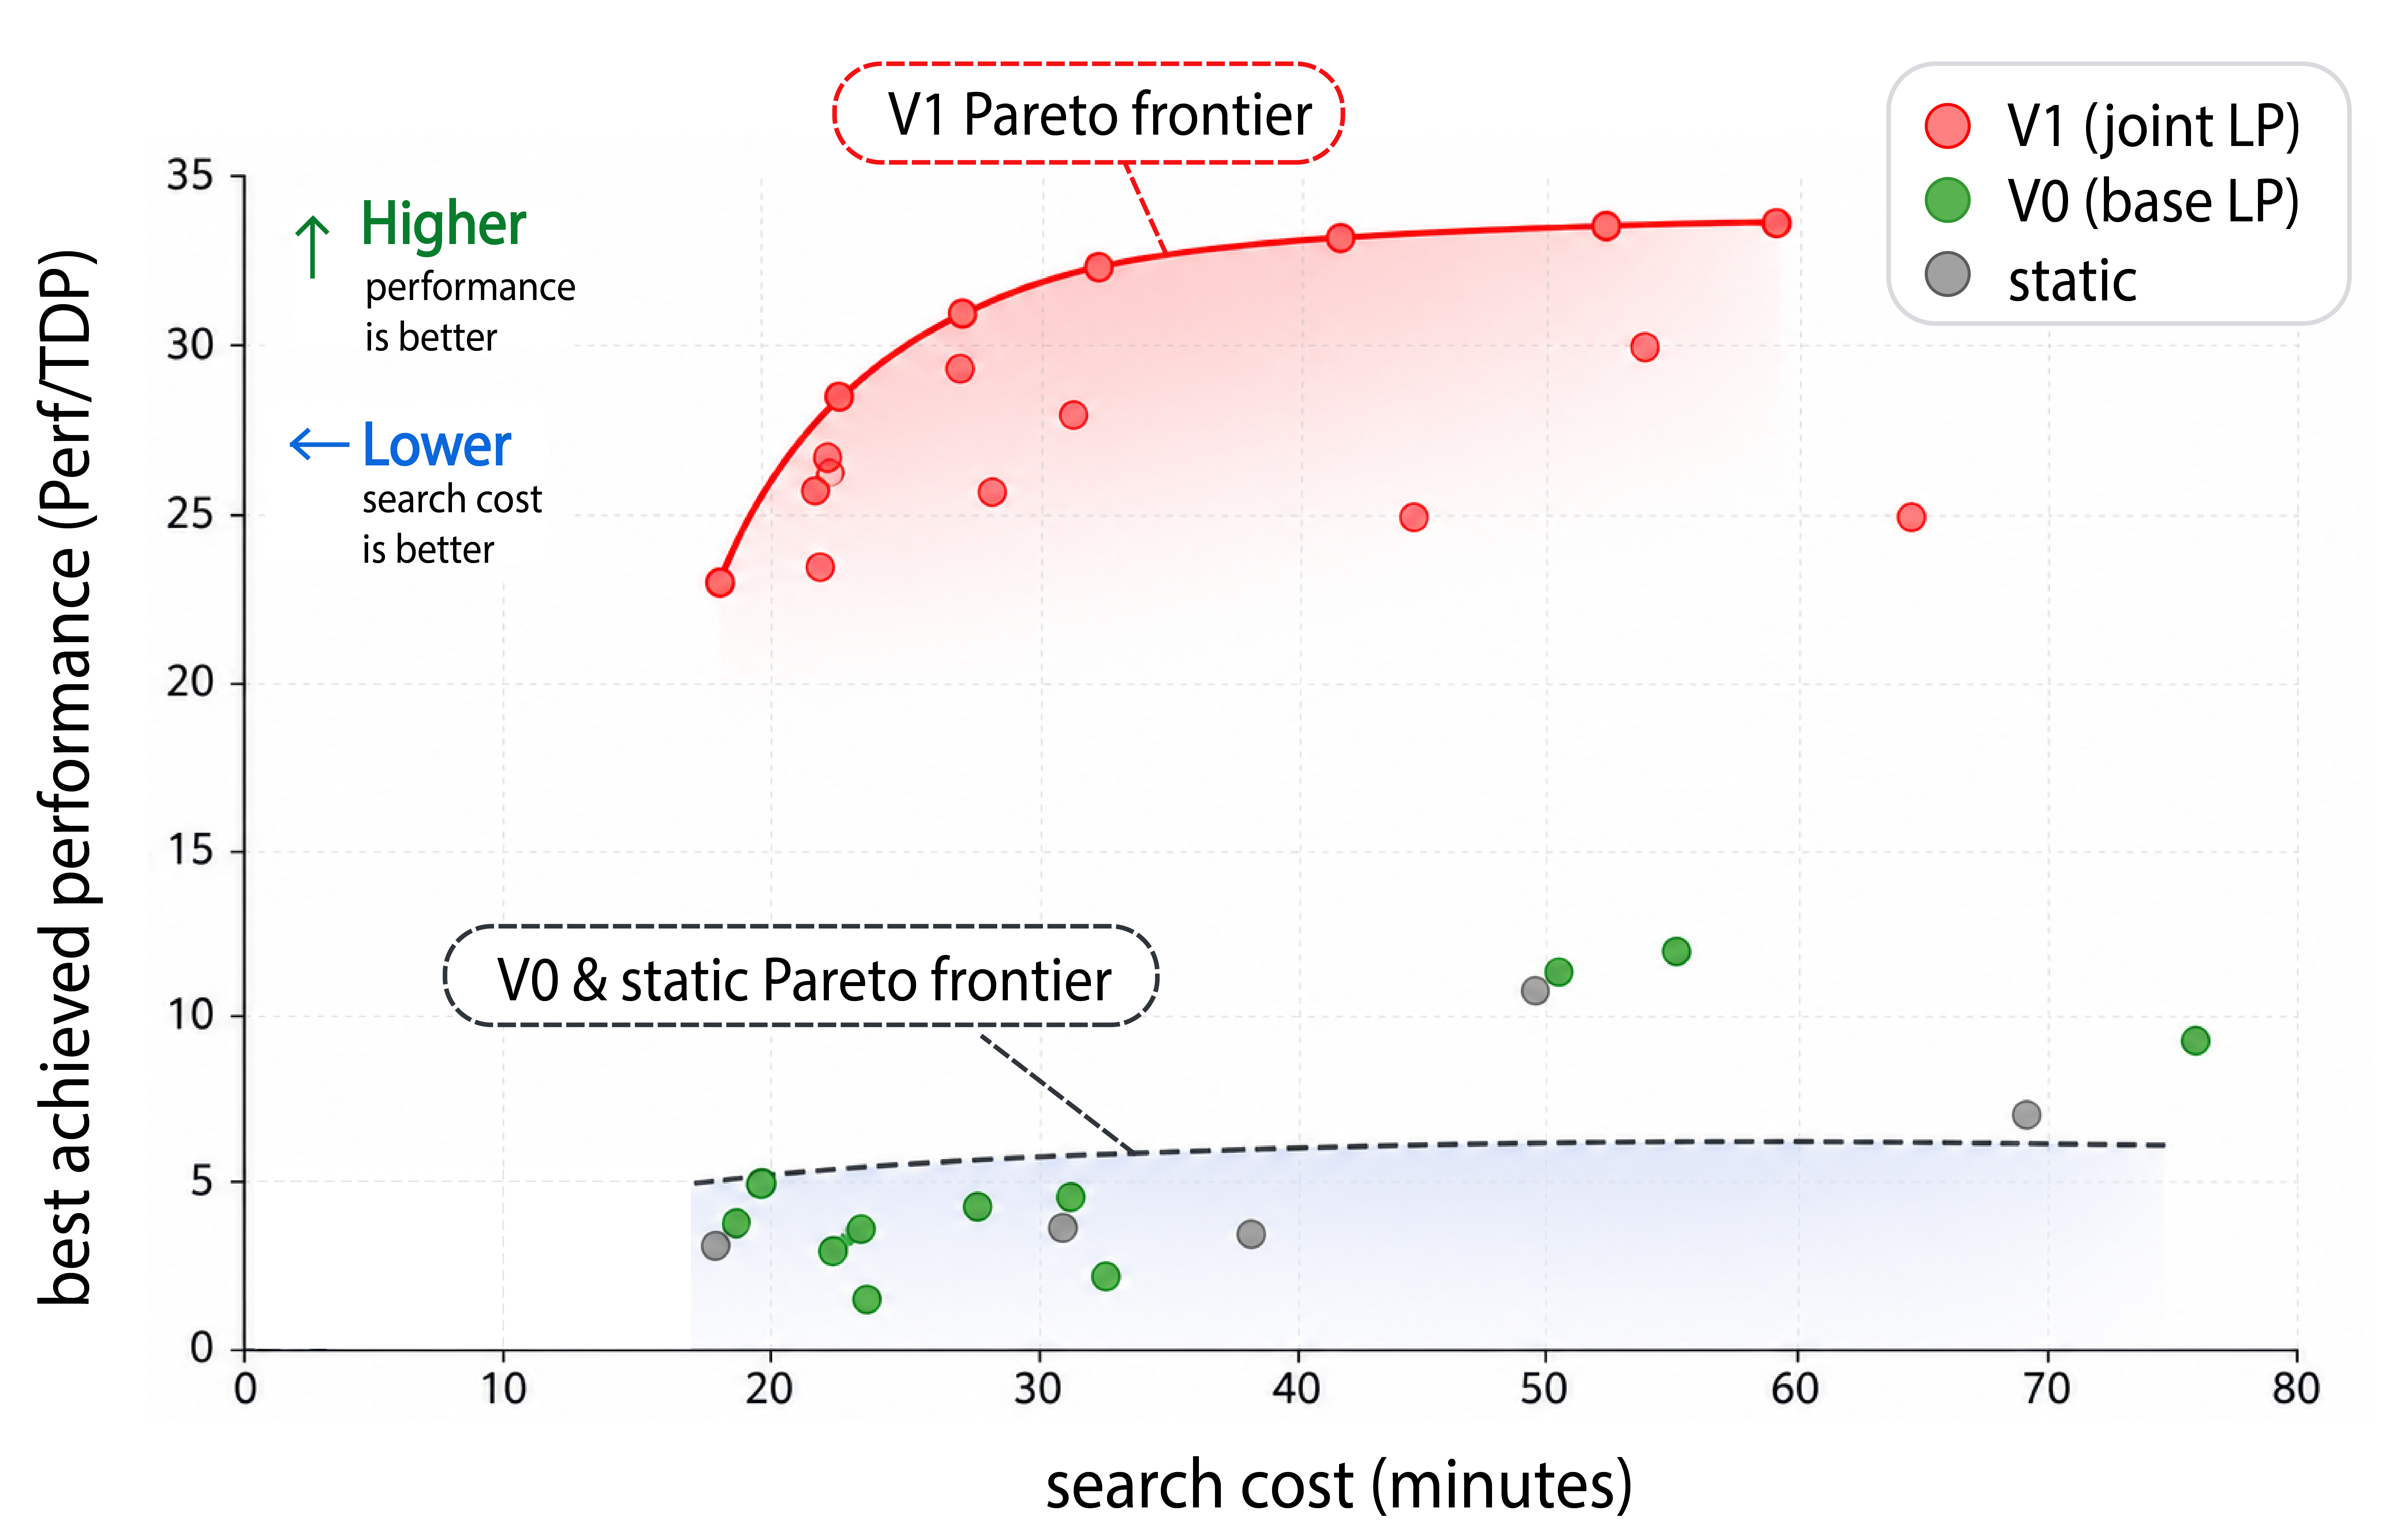
\includegraphics[width=0.7\linewidth]{figs/pareto_v2.png}
% % % %     \caption{pareto frontier plot}
% % % % \end{figure}
% % % \begin{figure}[ht!]
% % %     \centering
% % % 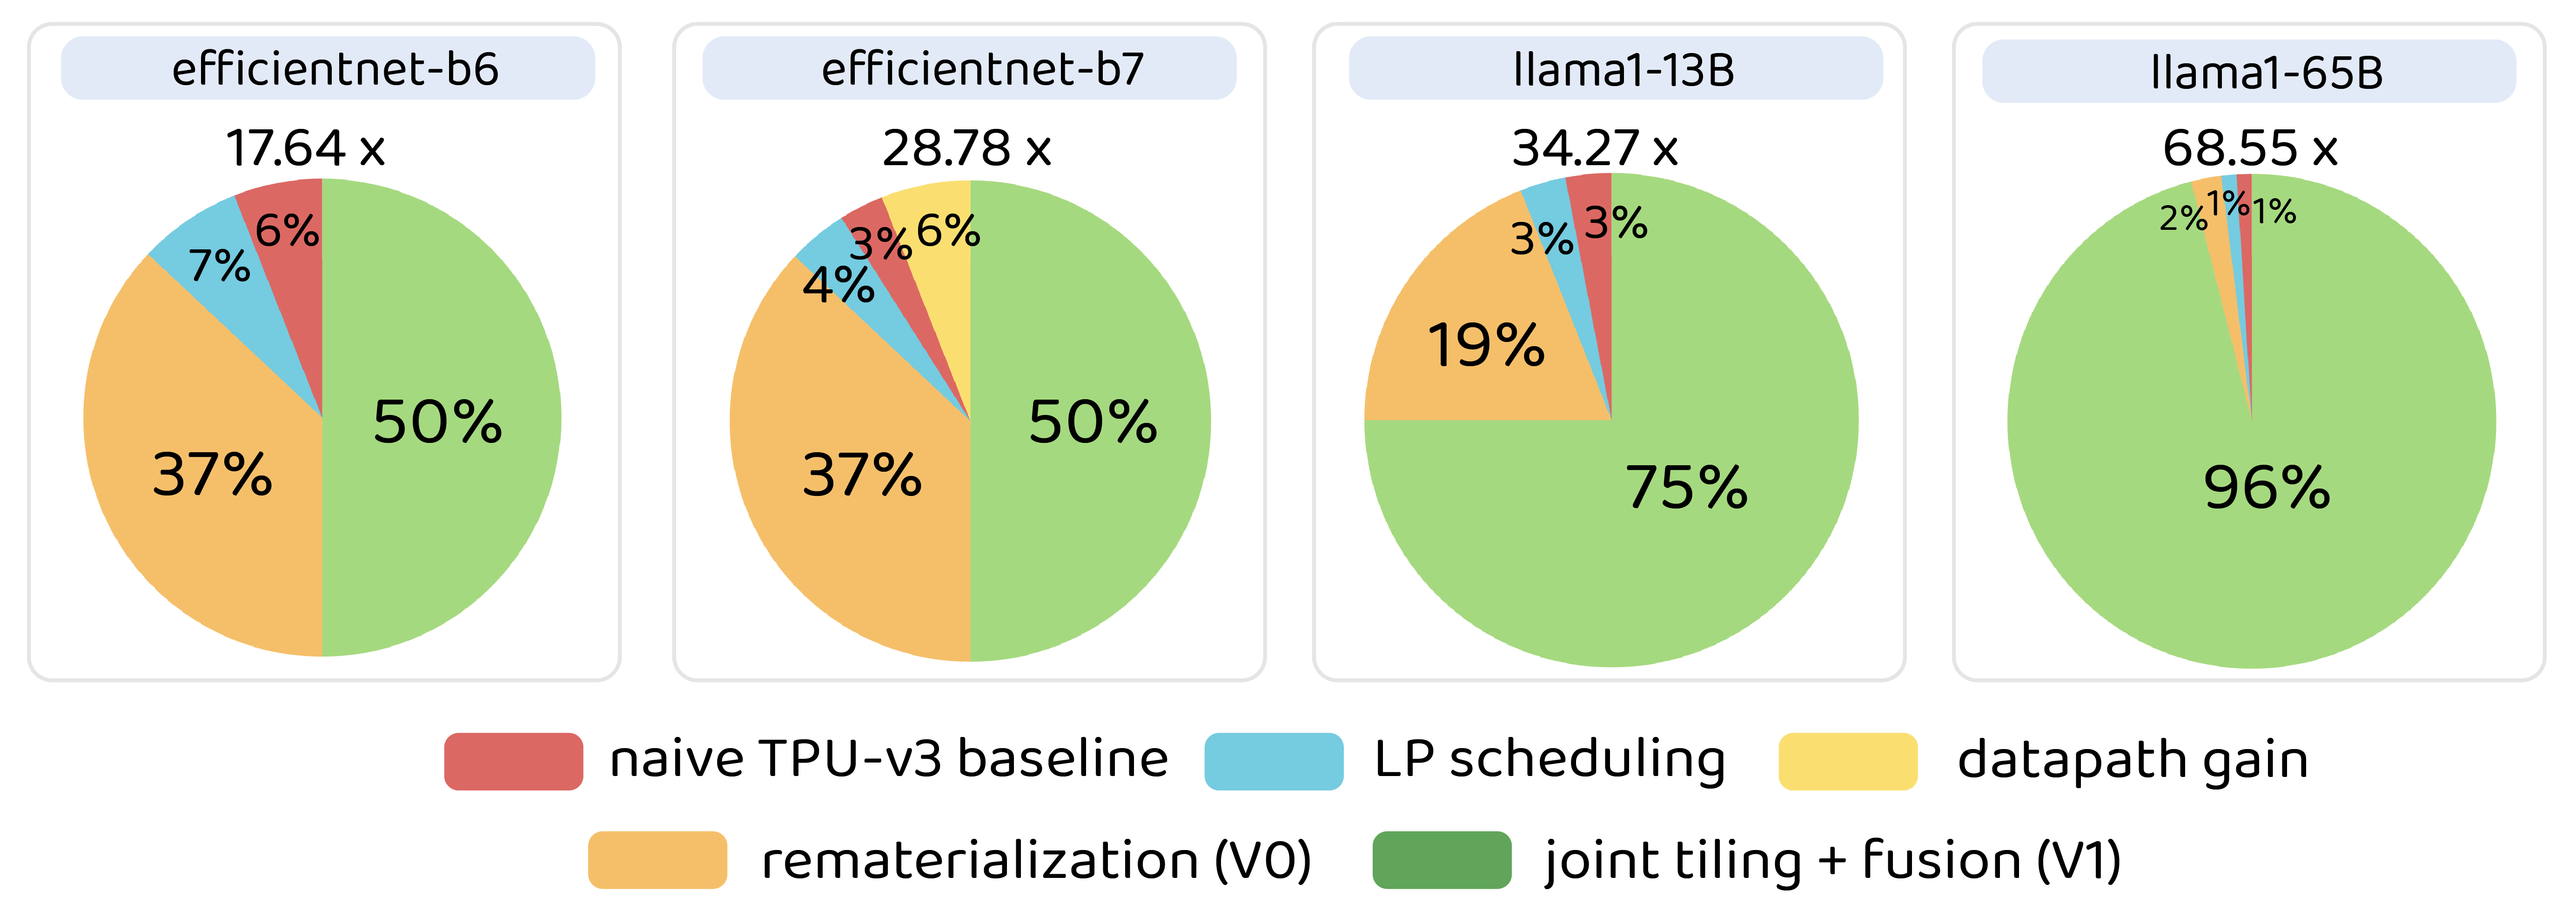
\includegraphics[width=0.85\linewidth]{fig3/speedup_decomposition_final_v2.png}
% % % \caption{Speedup decomposition over naive TPU-v3 baseline. Each pie shows the 
% % % relative contribution of four optimization sources to the total speedup. CHEETAH-V1 joint tiling + fusion dominates on all workloads, 
% % % especially on larger models where memory management is the primary bottleneck.}\label{fig:accel_decompose}
% % % \end{figure}
% % % \subsubsection{Static Baseline vs.\ CHEETAH-V0 vs.\ CHEETAH-V1 Unlock Progressive Gains}


% % % Figure~\ref{fig:accel_decompose} decomposes the total speedup over a naive TPU-v3 baseline into four sources: LP-based scheduling and fusion, datapath gain from hardware search, dynamic rematerialization (CHEETAH-V0), and joint tiling + fusion (CHEETAH-V1).

% % % The dominant contributor across all workloads is V1's joint tiling-fusion 
% % % optimization. On EfficientNet-B1, V1 accounts for 50\% of total speedup, 
% % % with LP scheduling (28\%) and datapath gain (22\%) splitting the remainder---and 
% % % no rematerialization benefit, consistent with B1's small activation footprint 
% % % fitting comfortably in Global Memory. B3--B4 show a similar 50\% V1 share, but 
% % % V0 rematerialization now contributes 25\%, reflecting the growing value of 
% % % recomputing large depthwise activations rather than reloading them from DRAM. 
% % % From B5 onward, V1's share rises sharply to 75--88\%, as the increasing 
% % % model size makes joint tiling-fusion the primary lever: memory management 
% % % dominates, and the remaining sources (LP scheduling, V0, datapath) each shrink 
% % % to single-digit percentages. The same pattern holds on Llama, where V1 accounts 
% % % for 83--87\% of the total speedup.

% % % % \begin{wrapfigure}{r}{0.48\textwidth}
% % % %     \centering
% % % %     \vspace{-12pt}
% % % %     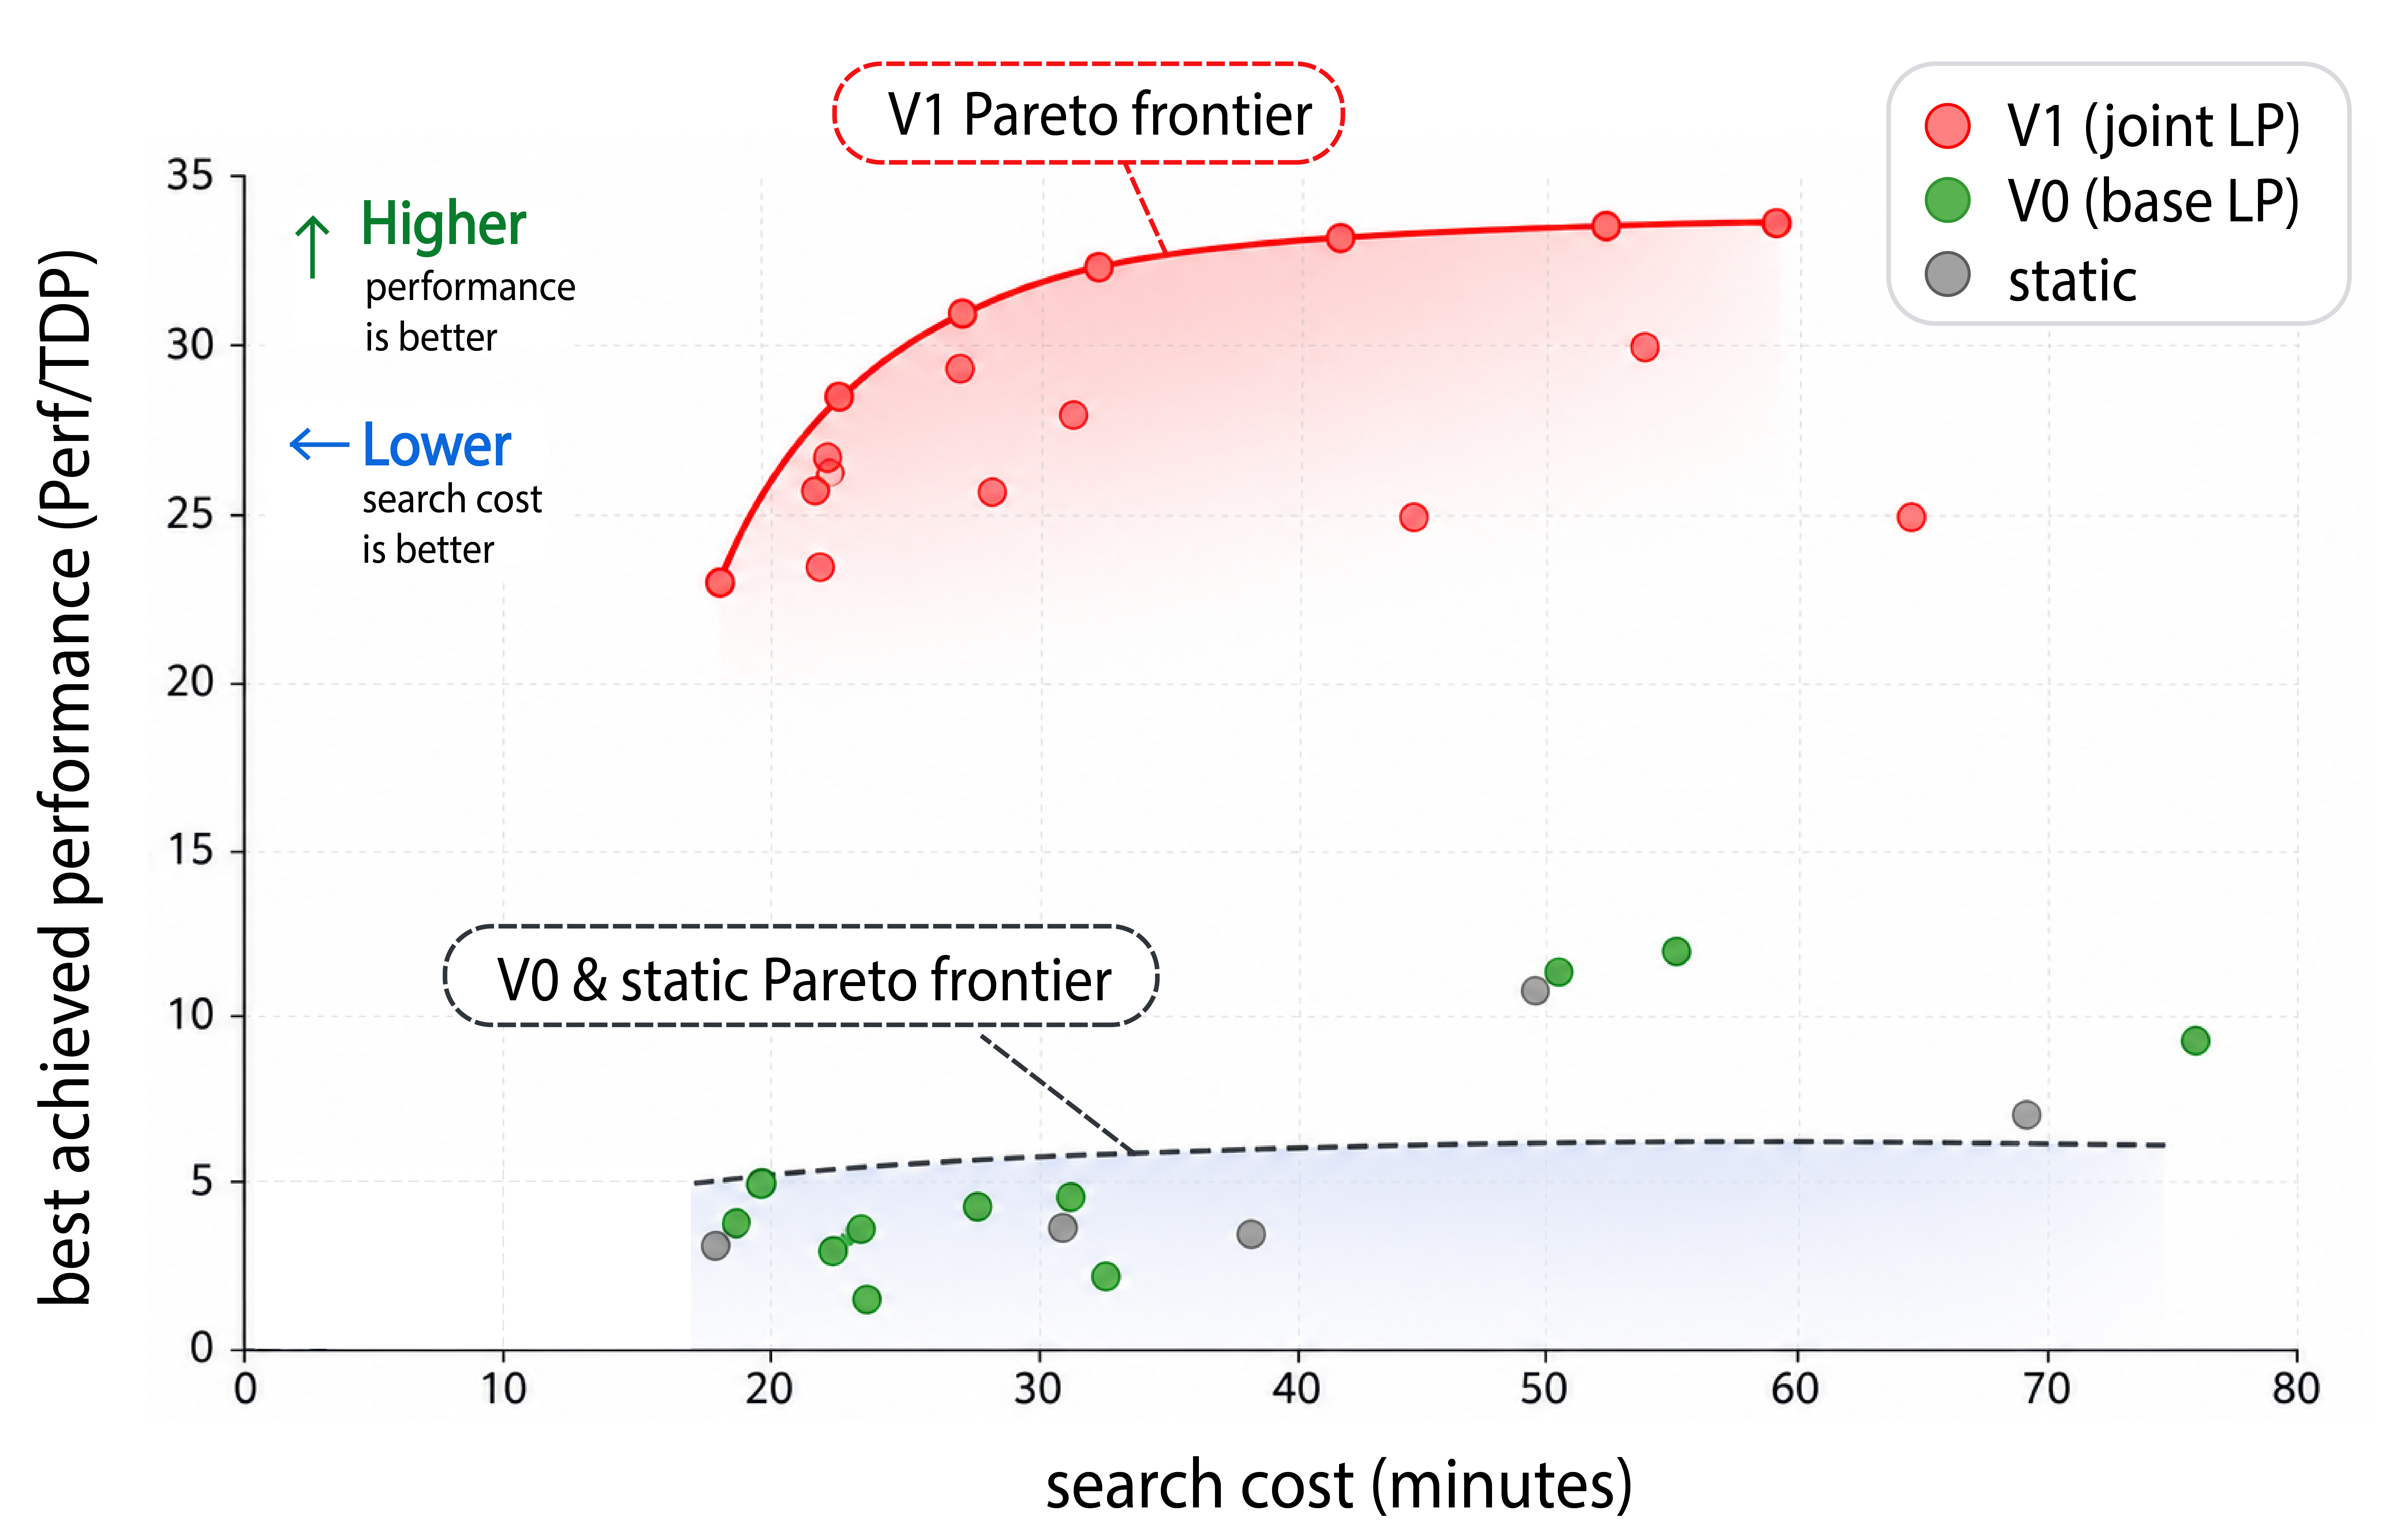
\includegraphics[width=0.48\textwidth]{figs/pareto_v2.png}
% % % %     \vspace{-18pt}
% % % %     \caption{Search cost vs.\ Perf/TDP Pareto frontier. V1 dominates V0 and static across all time budgets.}
% % % %     \label{fig:pareto}
% % % %     \vspace{-10pt}
% % % % \end{wrapfigure}

% % % Critically, Figure~\ref{fig:speedup} shows static fusion method is \emph{infeasible} on modern large models (Llama-70B, and DeepSeek-V3), because their large activation tensors cannot fit under a static pinning policy. The V0 formulation resolves feasibility for on large models via dynamic placement but remains time-intensive for a small number of 50 trials: measuring 58.42 hours on Llama-70B and 69.39 hours on DeepSeek-V3 (Figure~\ref{fig:wallclock}). In contrast Figures~\ref{fig:wallclock} and ~\ref{fig:speedup}, show the CHEETAH-V1 formulation out performs comparitive strategies in terms of speedup against the TPU-V3 baseline, and require only 1.17 hours on Llama-70B and 2.17 hours on DeepSeekv3 for 50 trails---a ${\sim}93\%$ average reduction. The powerful joint formulation is able to select memory-efficient tiling configurations alongside placement, achieving feasibility across the entire workload suite, demonstrating that joint optimization is not merely an incremental improvement but a qualitative capability unlock for large-scale models.

% % % % This demonstrates that by exploiting structural invariance and GPU-accelerated mathematical optimization, CHEETAH-V1 reduces the end-to-end co-design search time from days to under 2.2 hours—a ${\sim}93\%$ average reduction—while discovering architectural points that deliver up to $35\times$ speedup over the TPU-v3 baseline.

% % % % Figure~\ref{fig:pareto} shows the Pareto frontier of best-achieved Perf/TDP versus wall-clock search cost. V1 strictly dominates both V0 and static at every time budget: within 10 minutes of search, V1 already exceeds the best Perf/TDP that V0 or static achieve after 60+ minutes. The V1 Pareto frontier reaches ${\sim}35\times$ Perf/TDP, roughly $3\times$ higher than the V0/static frontier at ${\sim}10\text{--}12\times$. This gap reflects two compounding advantages: V1 explores a strictly larger feasible region (joint tiling-fusion), and it eliminates Timeloop from the per-trial critical path, allowing more trials within any fixed time budget.



% % % \paragraph{Practical insight.}
% % % Both LPs are extreme-aspect-ratio sparse: for \texttt{llama3\_70b},
% % % $m, n \sim 10^6$ and $\mathrm{nnz} \sim 5 \times 10^6$, giving roughly
% % % 1 nonzero per million matrix entries.
% % % The time-band structure means a coordinate-descent or stochastic PDHG
% % % solver would converge in $\mathcal{O}(T)$ sweeps if bands were the only
% % % structure.
% % % The capacity rows in both V0 and V1 LP formulations are the sole feature breaking strict banded structure, and they are precisely what couples the schedule globally. This is the desired behavior of a memory-aware placement formulation.

% % % % \todo{Report LP solve times for V0 and V1 across all benchmarks. Compare wall-clock time per trial against FAST's SCIP-based ILP solver (20 min timeout). Report LP relaxation gap: how often do fractional solutions need integer rounding, and what is the quality loss from rounding?}

% % % \paragraph{Structural invariance.}
% % % For a fixed workload and LP formulation, the LP constraint matrix
% % % has an invariant sparsity pattern across trials: the row/column
% % % dimensions and nonzero locations are determined only by the model graph structure — layer count $L$, timestep count $T$, edge set $E$, and Pareto count $C$ — not by the hardware candidate.
% % % Vizier changes only numerical values such as cycle coefficients,
% % % memory-capacity bounds, bandwidth-scaled access costs, objective weights, and TDP/area parameters. 
% % % This invariance allows us to reuse the same sparse matrix structure,
% % % variable ordering, block layout, and JIT-compiled sparse kernels in our adapted JAX PDLP solver across all hardware trials for a given workload.

% % % Numerically, we apply the same diagonal preconditioning pipeline
% % % on each trial: a structural presolve with 20 log-geomean Ruiz iterations, followed by the PDLP preprocessing stack with 10 infinity-norm Ruiz iterations and one Pock--Chambolle $\ell_1$-scaling pass. This two-stage diagonal scaling handles the mixed coefficient magnitudes present in V0/V1 matrices — large byte-valued capacity rows together with $\pm 1$ persistence rows — without requiring a fragile matrix factorization.

% % % In production, this preconditioning pipeline is reused structurally across trials, recomputes only cheap diagonal scalings, finishes in under one second for matrices with approximately $5 \times 10^6$ nonzeros, and avoids factorization failures entirely because it consists only of $D_1 A D_2$ arithmetic.

% % % \subsubsection{LLM Architect vs. Optimizer}
% % % The LLM Architect framework is modeled on SkyDiscover, and efficiently prunes the large outer hardware search loop by proposing campaign patches. Rather than predicting performance, the Architect reads a compact Causal Ledger containing invalid-rate history, MFU, roofline lower-bound checks, and LP diagnostics, then proposes a constrained hardware neighborhood for Vizier to search locally. The V1 LP remains the sole performance evaluator: for each candidate, it solves the joint tiling, fusion, placement, and rematerialization LP, while a deterministic Roofline Auditor rejects physically impossible results. In the widened V1 search space, all methods reach the same capped V1 Perf/TDP ceiling, so the key differentiator is search efficiency. The LLM loop reduces invalid hardware evaluations from 24.5\% under full-space Vizier to 5.9\% on average across five workloads, a 4.1× reduction in wasted trials, while preserving the same best V1 score. This shows that the LLM’s contribution is not replacing Vizier or the solver, but steering Bayesian optimization toward feasible, workload-appropriate architectural neighborhoods with far less wasted trials. This also sets the foundation for future work, where the LLM in the loop can adhere to follow more complex human reasoning signals.
% % % \begin{figure}[ht!]
% % %     \centering
% % % 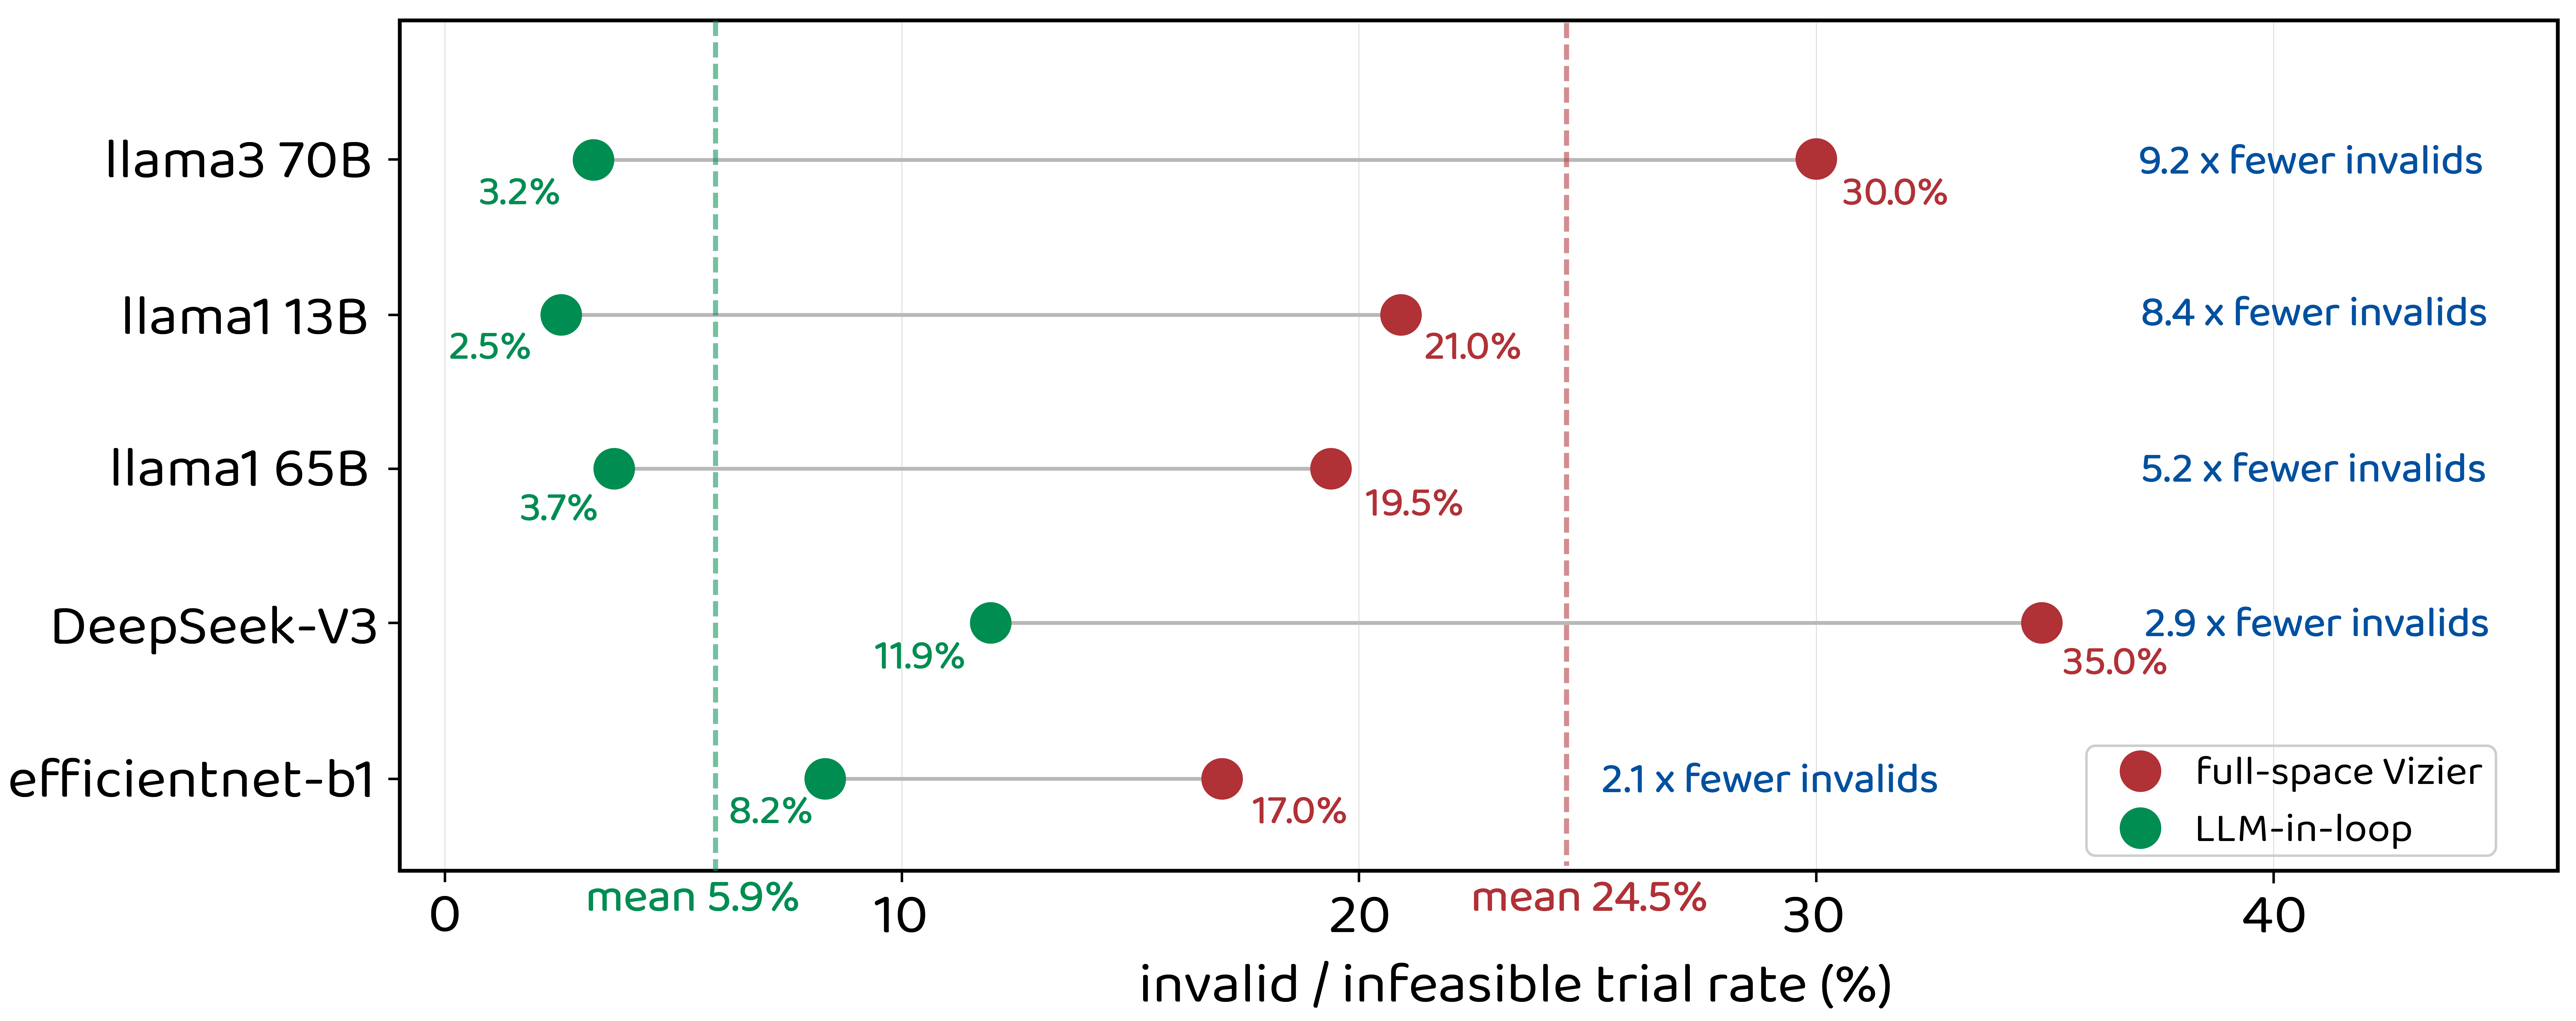
\includegraphics[width=0.85\linewidth]{fig3/llm_guide_v1.png}
% % % \caption{Strategic Intelligence vs. Stochastic Brute Force}\label{fig:llm}
% % % \end{figure}



% % % % The LLM should not just ask, “What chip has the best Perf/TDP?” We aim to answer the question “Given this user’s workload and deployment goal, what is the architectural region to search for this deployment task?”. Therefore we have the LLM emit profile-conditioned campaigns that take specific user inference tasks into consideration. For each $(\text{deployment profile},\ \text{workload})$ cell, we ran a
% % % % 200-trial LLM-Architect experiment using the same Qwen2.5-7B-Instruct + LoRA with differing user input profiles. At the start of each round, the prompt was assembled from a fixed system
% % % % prompt, the active deployment profile, three few-shot examples, and a per-round user message containing the workload, recent feedback signals, current search bounds, and the causal ledger.
% % % % The Strategist returned a one-line JSON campaign patch, which the
% % % % validator accepted only if it was a strict legal subset of the parent space, satisfied hard rules such as patch-volume $\leq 10\%$, ridgepoint and MAC/BW constraints, and avoided forbidden regions.

% % % % Thus, the experiment isolates whether the profile-conditioned LLM prompt alone can steer the same V1 evaluator toward different hardware families under different deployment intents.



% % % % \todo{Compare convergence rate of LLM-guided hardware search vs.\ Vizier-only (Bayesian, LCS, random baselines) in the style of FAST Figure~11. Report:
% % % % \begin{itemize}
% % % %     \item Number of trials to reach $X\%$ of best Perf/TDP found by 5,000-trial Vizier
% % % %     \item Quality of LLM-proposed configurations vs.\ Vizier-proposed configurations
% % % %     \item Qualitative analysis of LLM reasoning about hardware bottlenecks
% % % % \end{itemize}
% % % % }

% % % % \subsubsection{ROI Analysis}

% % % % \todo{Update FAST's ROI analysis (Table~4) with the improved Perf/TDP numbers from FAST-CORGI. Report deployment volumes required to reach 1$\times$, 2$\times$, 4$\times$ ROI targets. If Perf/TDP improvements are larger than FAST's, the break-even deployment volume should decrease correspondingly.}

% % % % \subsubsection{Pareto Frontier}

% % % % \todo{Plot the Perf/TDP vs.\ area Pareto frontier for V1-optimized designs compared to FAST and TPU-v3 baseline, analogous to FAST Figure~12.}


% % % edit for page limit

% % \section{Experiments}
% % \label{sec:experiments}
% % We implement an adapted JAX PDLP solver for large-scale models (Llama-70B and DeepSeek-V3) across all formulations (Static, V0, V1), while employing HiGHS for smaller networks. To maintain consistency with prior research, results are reported as speedup relative to a simulated TPU-v3 baseline. The TPU-v3 is selected as a benchmark because its architecture is purpose-built for neural network acceleration and its publicly available specifications permit high-fidelity simulation.

% % \subsection{Experimental Setup}

% % \paragraph{Static Sequential Baseline.}
% % We compare against the static optimization FAST framework using a simulated TPU-v3 baseline normalized to a sub-10nm process technology, following the same methodology as Zhang \etal. The baseline simulator is well-correlated with production hardware: on average within 8.2\,$\pm$\,2.7\% of profiled TPU-v3 performance. We evaluate against a \emph{simulated} TPU-v3 baseline to account for optimistic simulator assumptions. We evaluate across 11 representative workloads: EfficientNet-B1 through EfficientNet-B7, Llama13, 65, 70 models, and DeepSeek-V3-MoE. These workloads stress different parts of the hardware design space: EfficientNet stresses low-operational-intensity depthwise convolutions, while Llama and DeepSeek stress memory capacity, bandwidth, and large matrix operations. 

% % \textbf{Single-workload specialization.} Each neural network workload is optimized independently. This experiment measures the best workload-specific hardware found under a fixed trial budget and identifies architectural preferences such as Global Memory size, bandwidth, MAC count, and systolic shape. In the case of Staitic and V0 methods, the pipeline involves: Vizier - Timeloop - LP solver. In the case of the V1 method, the pipeline is simplified to Vizier - LP solver. In each case we iterate for 100 trials per method x NN. 

% % % \textbf{Fixed-hardware-workload generalization.} We search for general-purpose datapaths that perform well across the workload suite. The objective is a harmonic or geometric aggregation of per-workload Perf/TDP, forcing the search to balance CNN-style memory pressure and LLM-style compute/memory trade-offs.

% % \textbf{LLM-Architect guides outer search.} We the LLM-guided outer-loop controller which proposes search-space interventions for Vizier. The advantage of the CHEETAH-V1 formulation is it removes dependence of Timeloop in the loop. Therefore the loop is reduced to just Vizier-LP solve, which dramatically speeds up the iterative process, thus permitting the LLM-Architect outer loop. The LLM is only permitted to change the search neighborhood of Vizier's input, the strict LP formulation on the inner loop does not change. This ensures mathematical and physical constraints are upheld in the space of co-design. We validate all results through a multi-level audit process---Roofline Auditor, Campaign Validator, Causal Ledger, and solver diagnostics (primal/dual residuals, duality gap)---as described in Section~\ref{sec:llm_outer} and detailed in Appendix~\ref{app:validation}. All reported V0/V1 results are roofline-feasible with zero lower-bound violations.

% % % \paragraph{Optimization framework.}
% % % For the outer hardware search loop, we use Google Vizier with LCS optimization and safe search, running 100 trials per experiment (method X NN x Exp). Each trial invokes the LP solver for the inner optimization. The Static and V0 methods additionally have Timeloop in the loop (Vizier-Timeloop-LP solve). The advantage of the v1 formulation is it removes dependance of Timeloop in the loop. Therefore the loop is reduced to just Vizier-Lp solve, which dramatically speeds up the iterative process, thus permitted the Strategic LLM outer loop.




% % \subsection{Main Results}

% % % \subsubsection{V0 vs.\ FAST Static Fusion}

% % % \todo{Insert results table and figure comparing V0 (time-indexed placement + rematerialization) against FAST's static fusion ILP on all benchmarks. Key metrics: Perf/TDP improvement, fusion efficiency (\% of DRAM stall time eliminated), rematerialization frequency (how often does the solver choose to recompute rather than reload?).}

% % % \paragraph{Expected findings.}
% % % V0's dynamic placement should show the largest gains on workloads with: (1)~tight Global Memory budgets where static pinning wastes capacity on tensors that are only needed briefly, (2)~long dependency chains where tensor lifetimes vary substantially, and (3)~cheap-to-recompute operations with large activations (\eg, depthwise convolutions in EfficientNet).

% % % \subsubsection{V1 vs.\ V0: Joint Tiling and Fusion}

% % % \todo{Insert results table and figure comparing V1 against V0 on all benchmarks. Key metrics: Perf/TDP improvement, number of operations where V1 selects a different tiling configuration than Timeloop's greedy choice, and the resulting compute efficiency vs.\ fusion trade-off.}

% % % \paragraph{Expected findings.}
% % % V1 should show the largest gains on architectures with highly diverse layer types where a single tiling configuration cannot serve all operations well. EfficientNet (depthwise + pointwise convolutions with 100$\times$ variation in working-set sizes) and hybrid CNN-transformer models (convolutions + attention + MLP with fundamentally different compute-memory profiles) are expected to benefit most.


% % % \subsubsection{stiatic vs v0 vs v1}
% % % \begin{figure}[ht!]
% % %     \centering
% % %     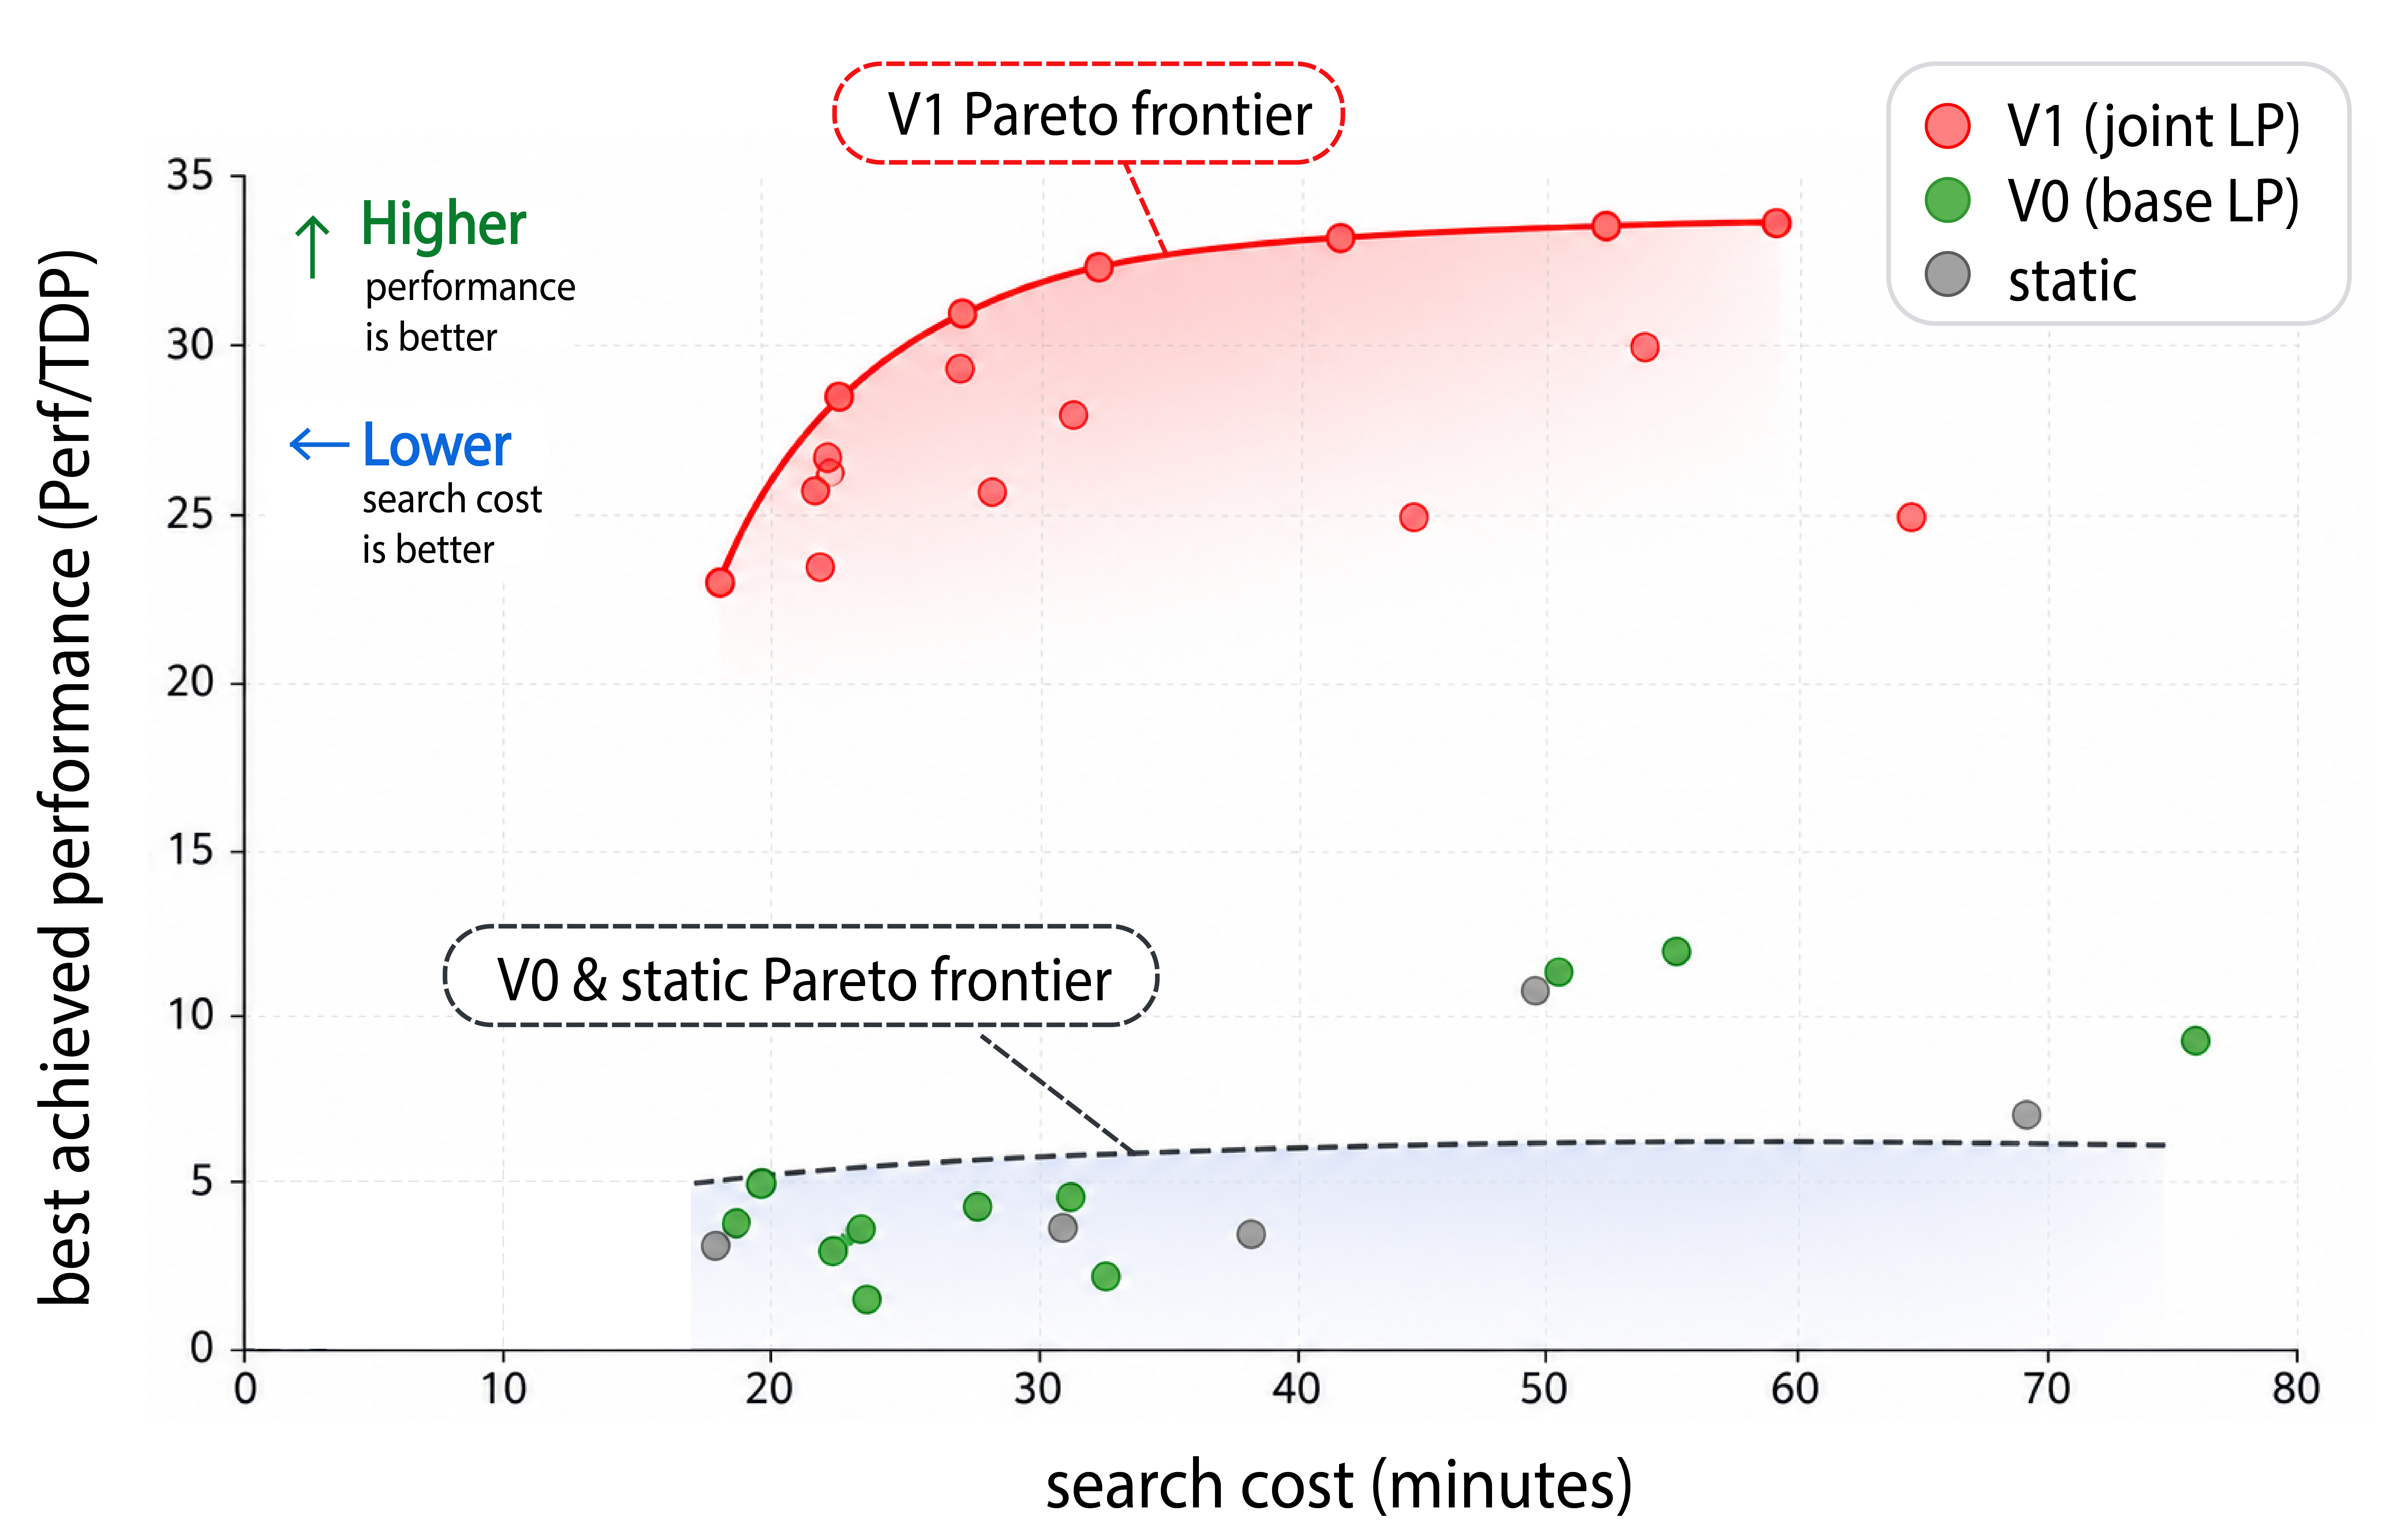
\includegraphics[width=0.7\linewidth]{figs/pareto_v2.png}
% % %     \caption{pareto frontier plot}
% % % \end{figure}
% % \begin{figure}[ht!]
% %     \centering
% % 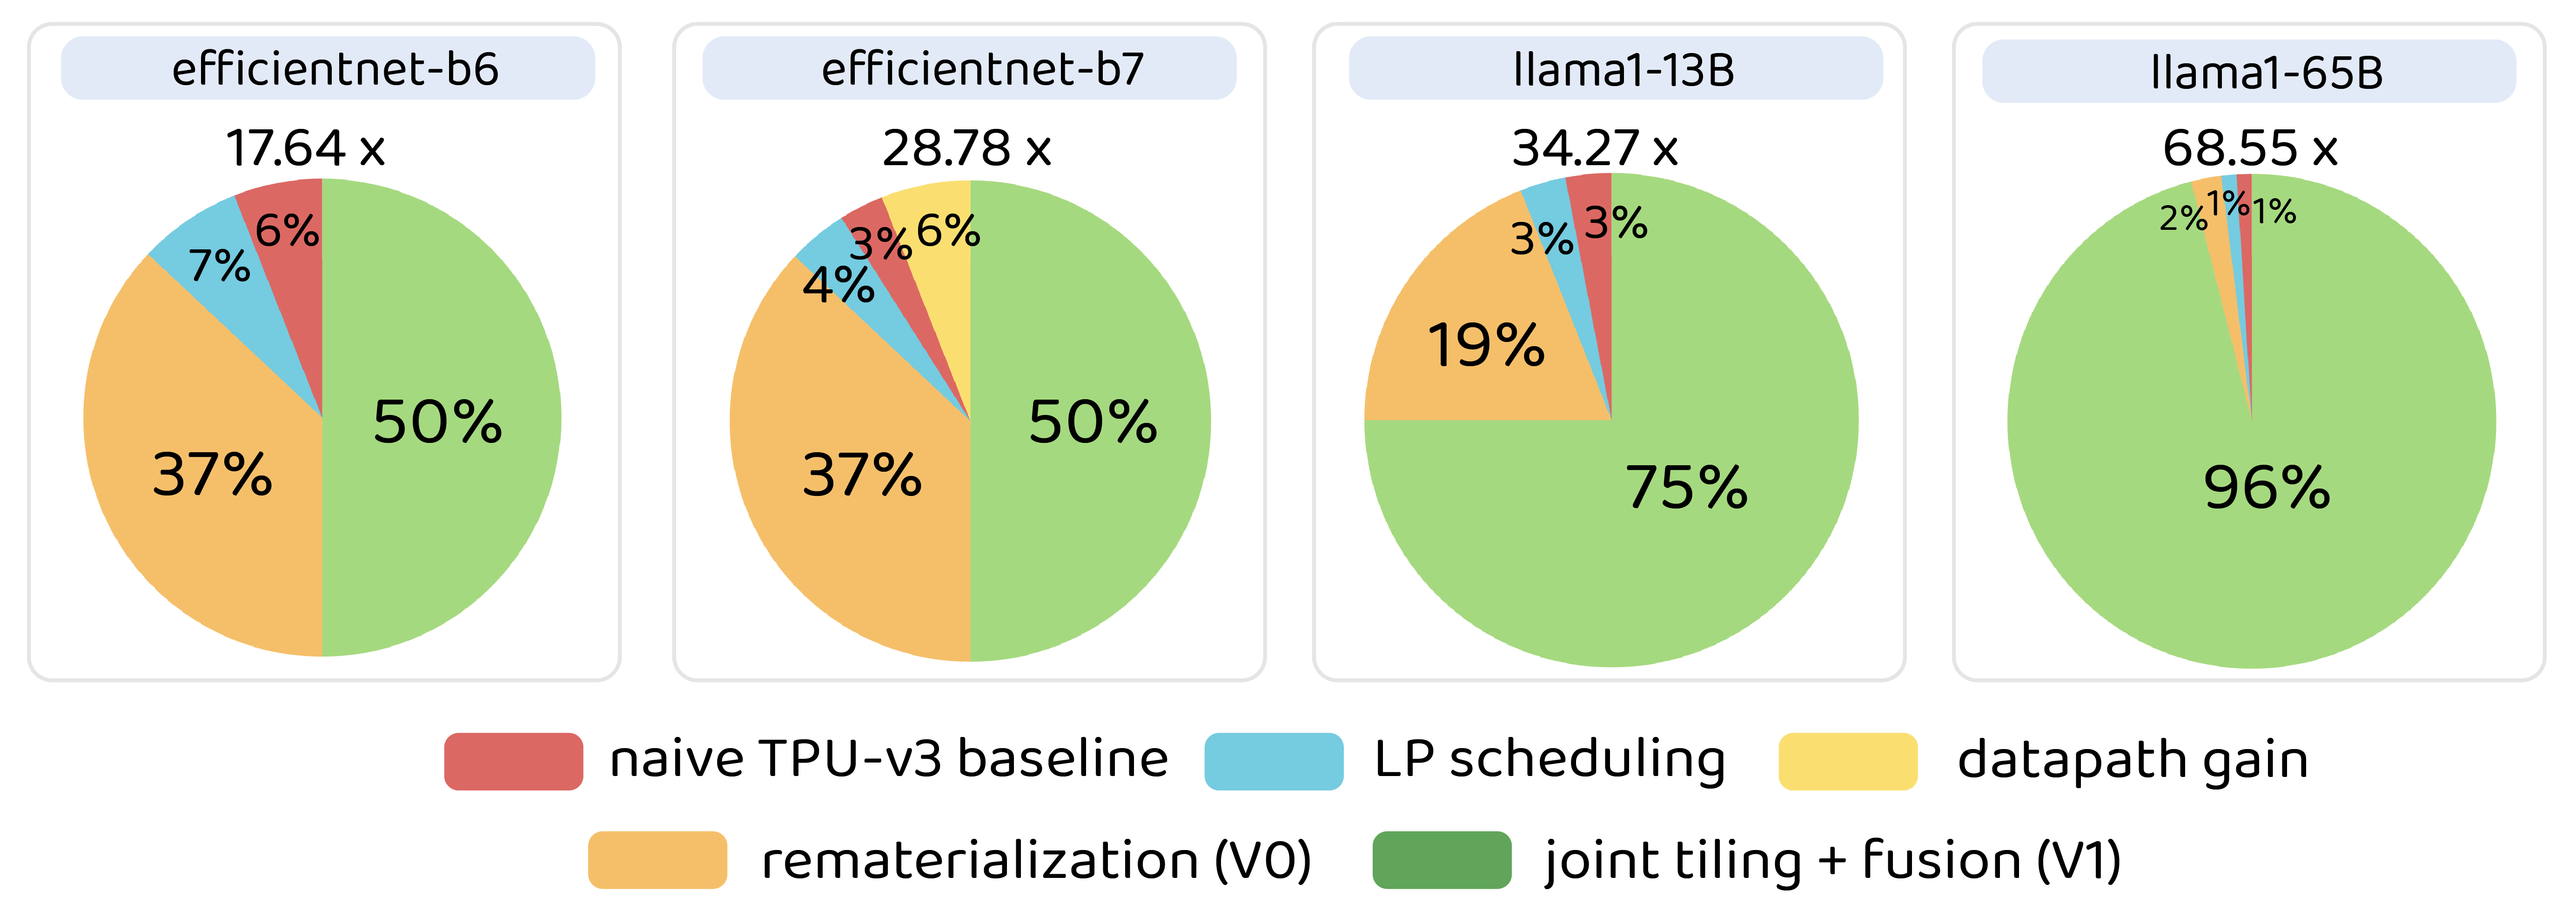
\includegraphics[width=0.85\linewidth]{fig3/speedup_decomposition_final_v2.png}
% % \caption{Speedup decomposition over naive TPU-v3 baseline. Each pie shows the 
% % relative contribution of four optimization sources to the total speedup. CHEETAH-V1 joint tiling + fusion dominates on all workloads, 
% % especially on larger models where memory management is the primary bottleneck.}\label{fig:accel_decompose}
% % \end{figure}
% % \paragraph{CHEETAH-V0 vs.\ CHEETAH-V1 Unlock Progressive Gains.} Figure~\ref{fig:accel_decompose} decomposes the total speedup over a naive TPU-v3 baseline into four sources: LP-based scheduling and fusion, datapath gain from hardware search, dynamic rematerialization (CHEETAH-V0), and joint tiling + fusion (CHEETAH-V1).

% % The dominant contributor across all workloads is V1's joint tiling-fusion 
% % optimization. On EfficientNet-B1, V1 accounts for 50\% of total speedup, 
% % with LP scheduling (28\%) and datapath gain (22\%) splitting the remainder---and 
% % no rematerialization benefit, consistent with B1's small activation footprint 
% % fitting comfortably in Global Memory. B3--B4 show a similar 50\% V1 share, but 
% % V0 rematerialization now contributes 25\%, reflecting the growing value of 
% % recomputing large depthwise activations rather than reloading them from DRAM. 
% % From B5 onward, V1's share rises sharply to 75--88\%, as the increasing 
% % model size makes joint tiling-fusion the primary lever: memory management 
% % dominates, and the remaining sources (LP scheduling, V0, datapath) each shrink 
% % to single-digit percentages. The same pattern holds on Llama, where V1 accounts 
% % for 83--87\% of the total speedup.

% % % \begin{wrapfigure}{r}{0.48\textwidth}
% % %     \centering
% % %     \vspace{-12pt}
% % %     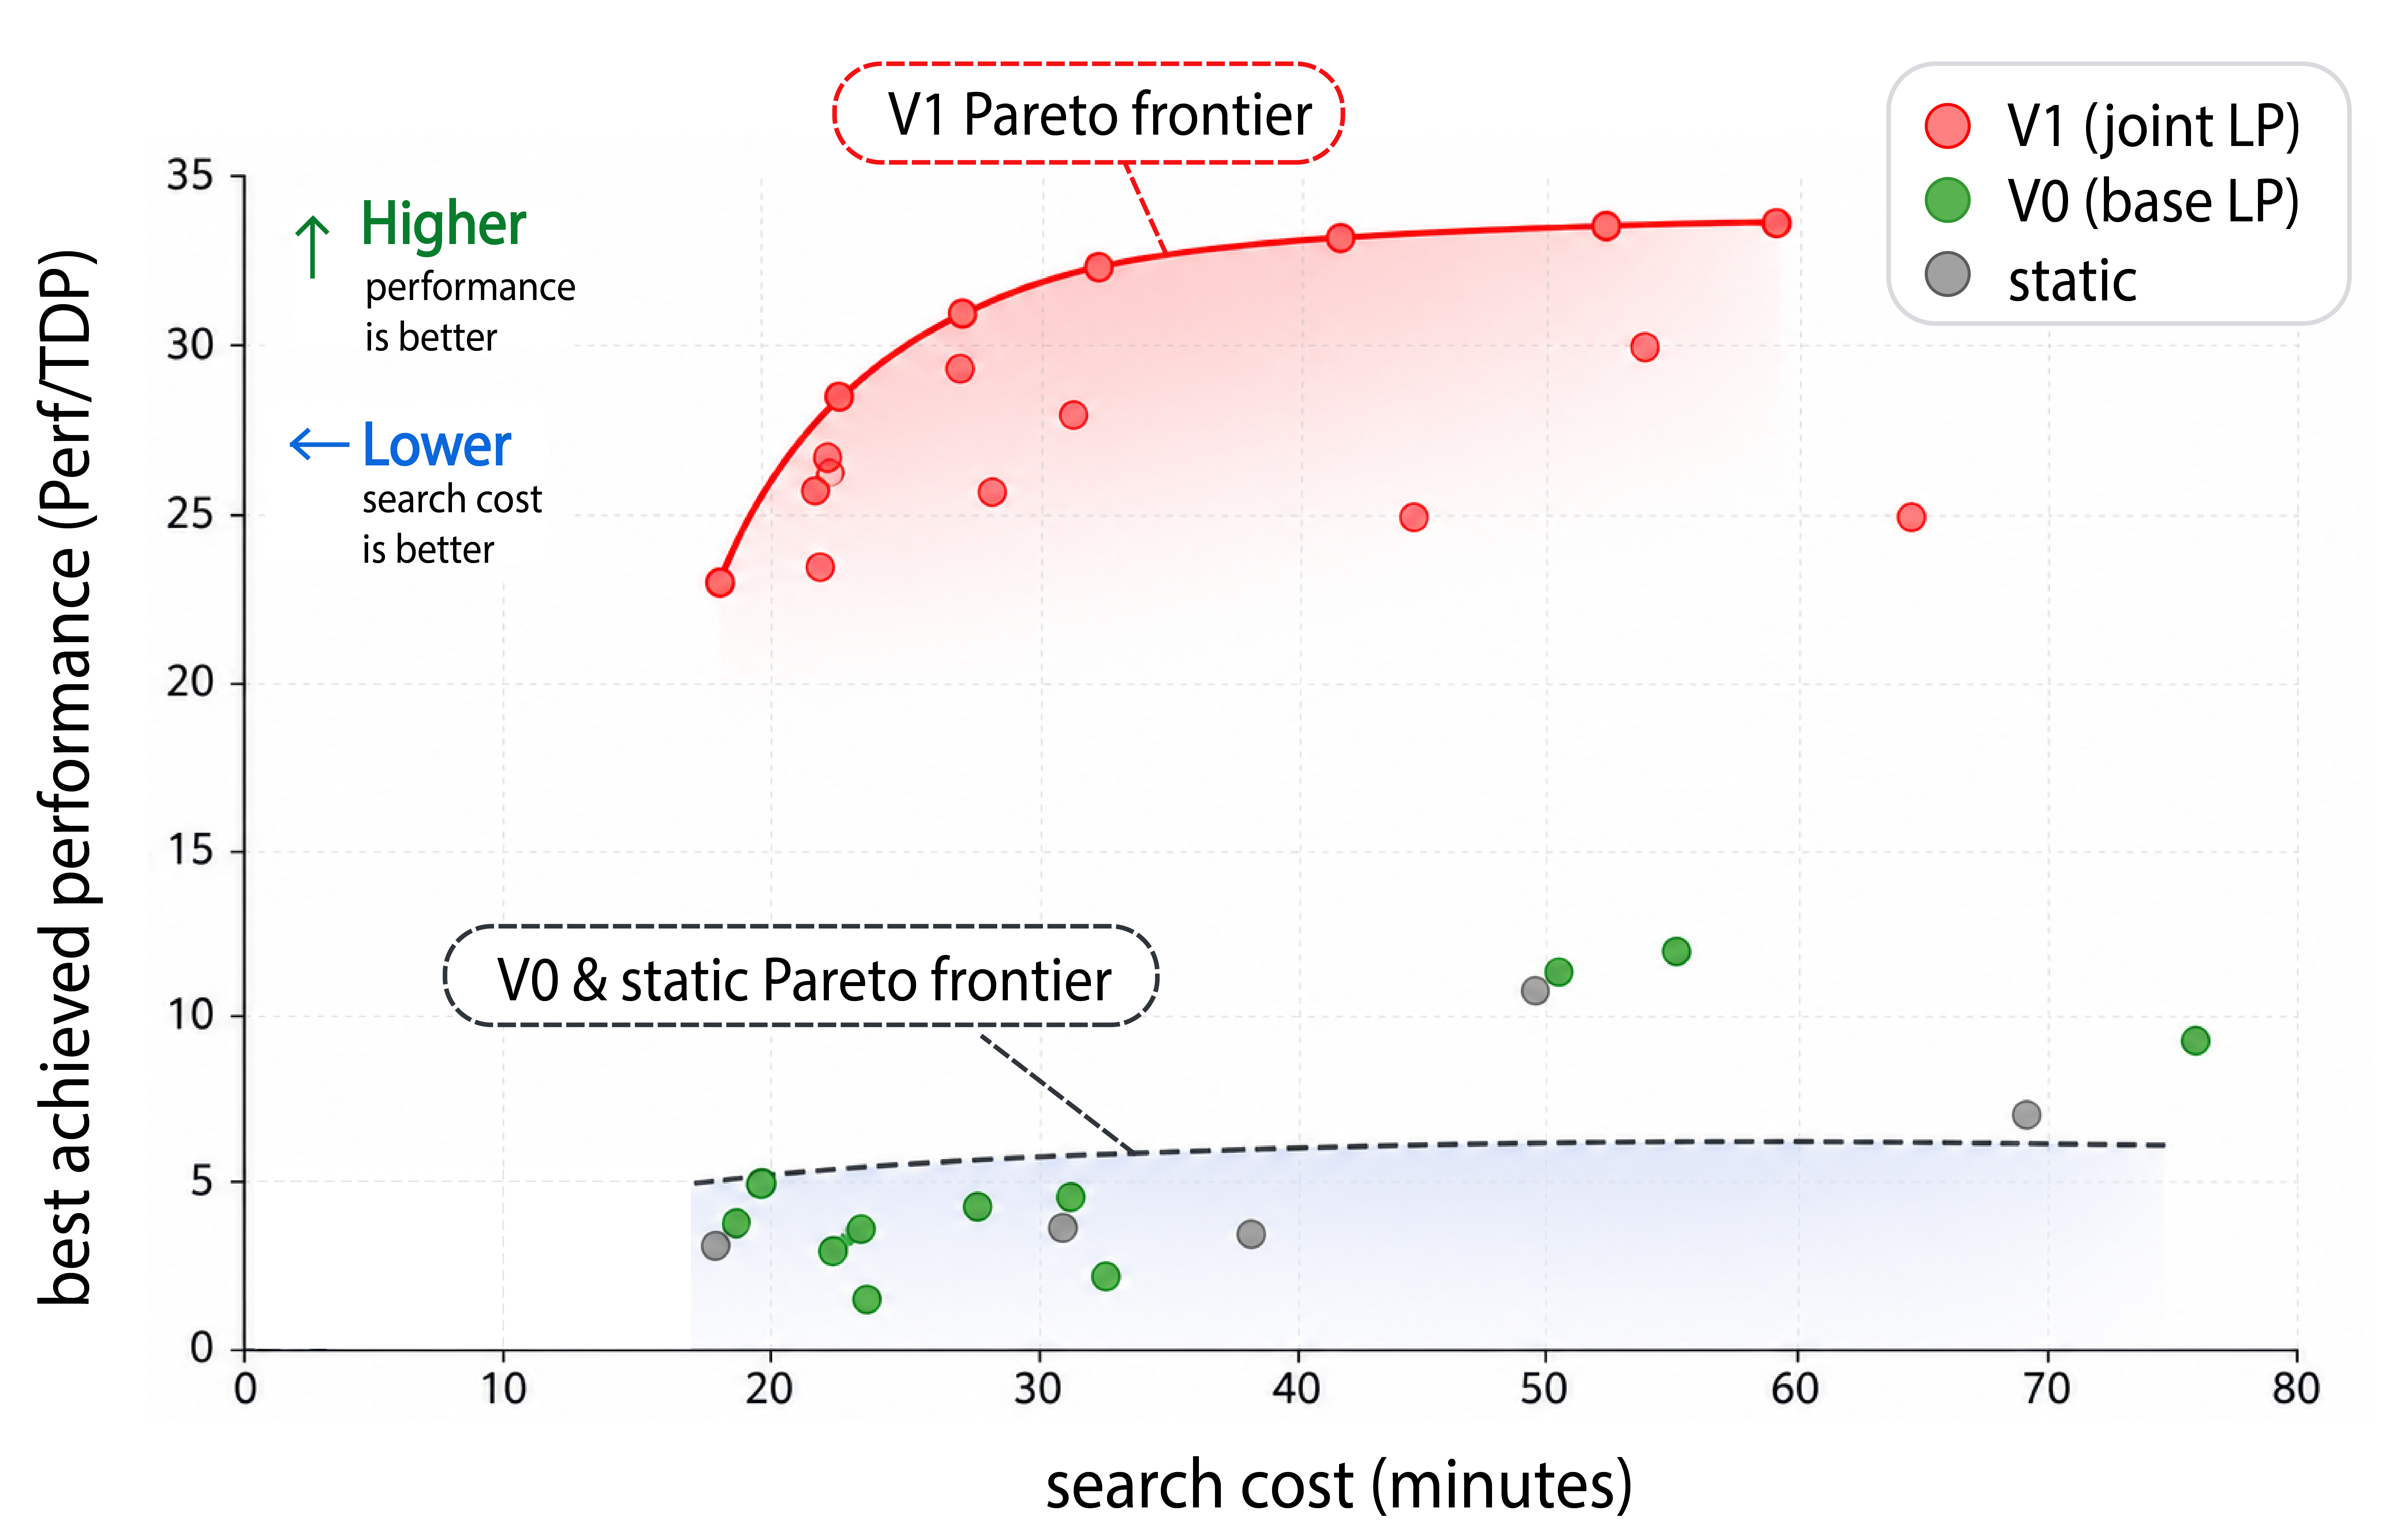
\includegraphics[width=0.48\textwidth]{figs/pareto_v2.png}
% % %     \vspace{-18pt}
% % %     \caption{Search cost vs.\ Perf/TDP Pareto frontier. V1 dominates V0 and static across all time budgets.}
% % %     \label{fig:pareto}
% % %     \vspace{-10pt}
% % % \end{wrapfigure}

% % Critically, Figure~\ref{fig:speedup} shows static fusion method is \emph{infeasible} on modern large models (Llama-70B, and DeepSeek-V3), because their large activation tensors cannot fit under a static pinning policy. The V0 formulation resolves feasibility for on large models via dynamic placement but remains time-intensive for a small number of 50 trials: measuring 58.42 hours on Llama-70B and 69.39 hours on DeepSeek-V3 (Figure~\ref{fig:wallclock}). In contrast Figures~\ref{fig:wallclock} and ~\ref{fig:speedup}, show the CHEETAH-V1 formulation out performs comparitive strategies in terms of speedup against the TPU-V3 baseline, and require only 1.17 hours on Llama-70B and 2.17 hours on DeepSeekv3 for 50 trails---a ${\sim}93\%$ average reduction. The powerful joint formulation is able to select memory-efficient tiling configurations alongside placement, achieving feasibility across the entire workload suite, demonstrating that joint optimization is not merely an incremental improvement but a qualitative capability unlock for large-scale models.

% % % This demonstrates that by exploiting structural invariance and GPU-accelerated mathematical optimization, CHEETAH-V1 reduces the end-to-end co-design search time from days to under 2.2 hours—a ${\sim}93\%$ average reduction—while discovering architectural points that deliver up to $35\times$ speedup over the TPU-v3 baseline.

% % % Figure~\ref{fig:pareto} shows the Pareto frontier of best-achieved Perf/TDP versus wall-clock search cost. V1 strictly dominates both V0 and static at every time budget: within 10 minutes of search, V1 already exceeds the best Perf/TDP that V0 or static achieve after 60+ minutes. The V1 Pareto frontier reaches ${\sim}35\times$ Perf/TDP, roughly $3\times$ higher than the V0/static frontier at ${\sim}10\text{--}12\times$. This gap reflects two compounding advantages: V1 explores a strictly larger feasible region (joint tiling-fusion), and it eliminates Timeloop from the per-trial critical path, allowing more trials within any fixed time budget.



% % \paragraph{Practical insight.}
% % Both LPs are extreme-aspect-ratio sparse: for \texttt{llama3\_70b},
% % $m, n \sim 10^6$ and $\mathrm{nnz} \sim 5 \times 10^6$, giving roughly
% % 1 nonzero per million matrix entries.
% % The time-band structure means a coordinate-descent or stochastic PDHG
% % solver would converge in $\mathcal{O}(T)$ sweeps if bands were the only
% % structure.
% % The capacity rows in both V0 and V1 LP formulations are the sole feature breaking strict banded structure, and they are precisely what couples the schedule globally. This is the desired behavior of a memory-aware placement formulation.

% % % \todo{Report LP solve times for V0 and V1 across all benchmarks. Compare wall-clock time per trial against FAST's SCIP-based ILP solver (20 min timeout). Report LP relaxation gap: how often do fractional solutions need integer rounding, and what is the quality loss from rounding?}

% % \paragraph{Structural invariance.}
% % For a fixed workload and LP formulation, the LP constraint matrix
% % has an invariant sparsity pattern across trials: the row/column
% % dimensions and nonzero locations are determined only by the model graph structure — layer count $L$, timestep count $T$, edge set $E$, and Pareto count $C$ — not by the hardware candidate.
% % Vizier changes only numerical values such as cycle coefficients,
% % memory-capacity bounds, bandwidth-scaled access costs, objective weights, and TDP/area parameters. 
% % This invariance allows us to reuse the same sparse matrix structure,
% % variable ordering, block layout, and JIT-compiled sparse kernels in our adapted JAX PDLP solver across all hardware trials for a given workload. We apply the same diagonal preconditioning pipeline
% % on each trial: a structural presolve with 20 log-geomean Ruiz iterations, followed by the PDLP preprocessing stack with 10 infinity-norm Ruiz iterations and one Pock--Chambolle $\ell_1$-scaling pass. This two-stage diagonal scaling handles the mixed coefficient magnitudes present in V0/V1 matrices — large byte-valued capacity rows together with $\pm 1$ persistence rows — without requiring a fragile matrix factorization. In production, this preconditioning pipeline is reused structurally across trials, recomputes only cheap diagonal scalings, finishes in under one second for matrices with approximately $5 \times 10^6$ nonzeros, and avoids factorization failures entirely because it consists only of $D_1 A D_2$ arithmetic.

% % \paragraph{LLM Architect vs.\ Optimizer.} 
% % \begin{wrapfigure}{r}{0.50\textwidth}
% %     \centering
% %     \vspace{-6pt}
% %     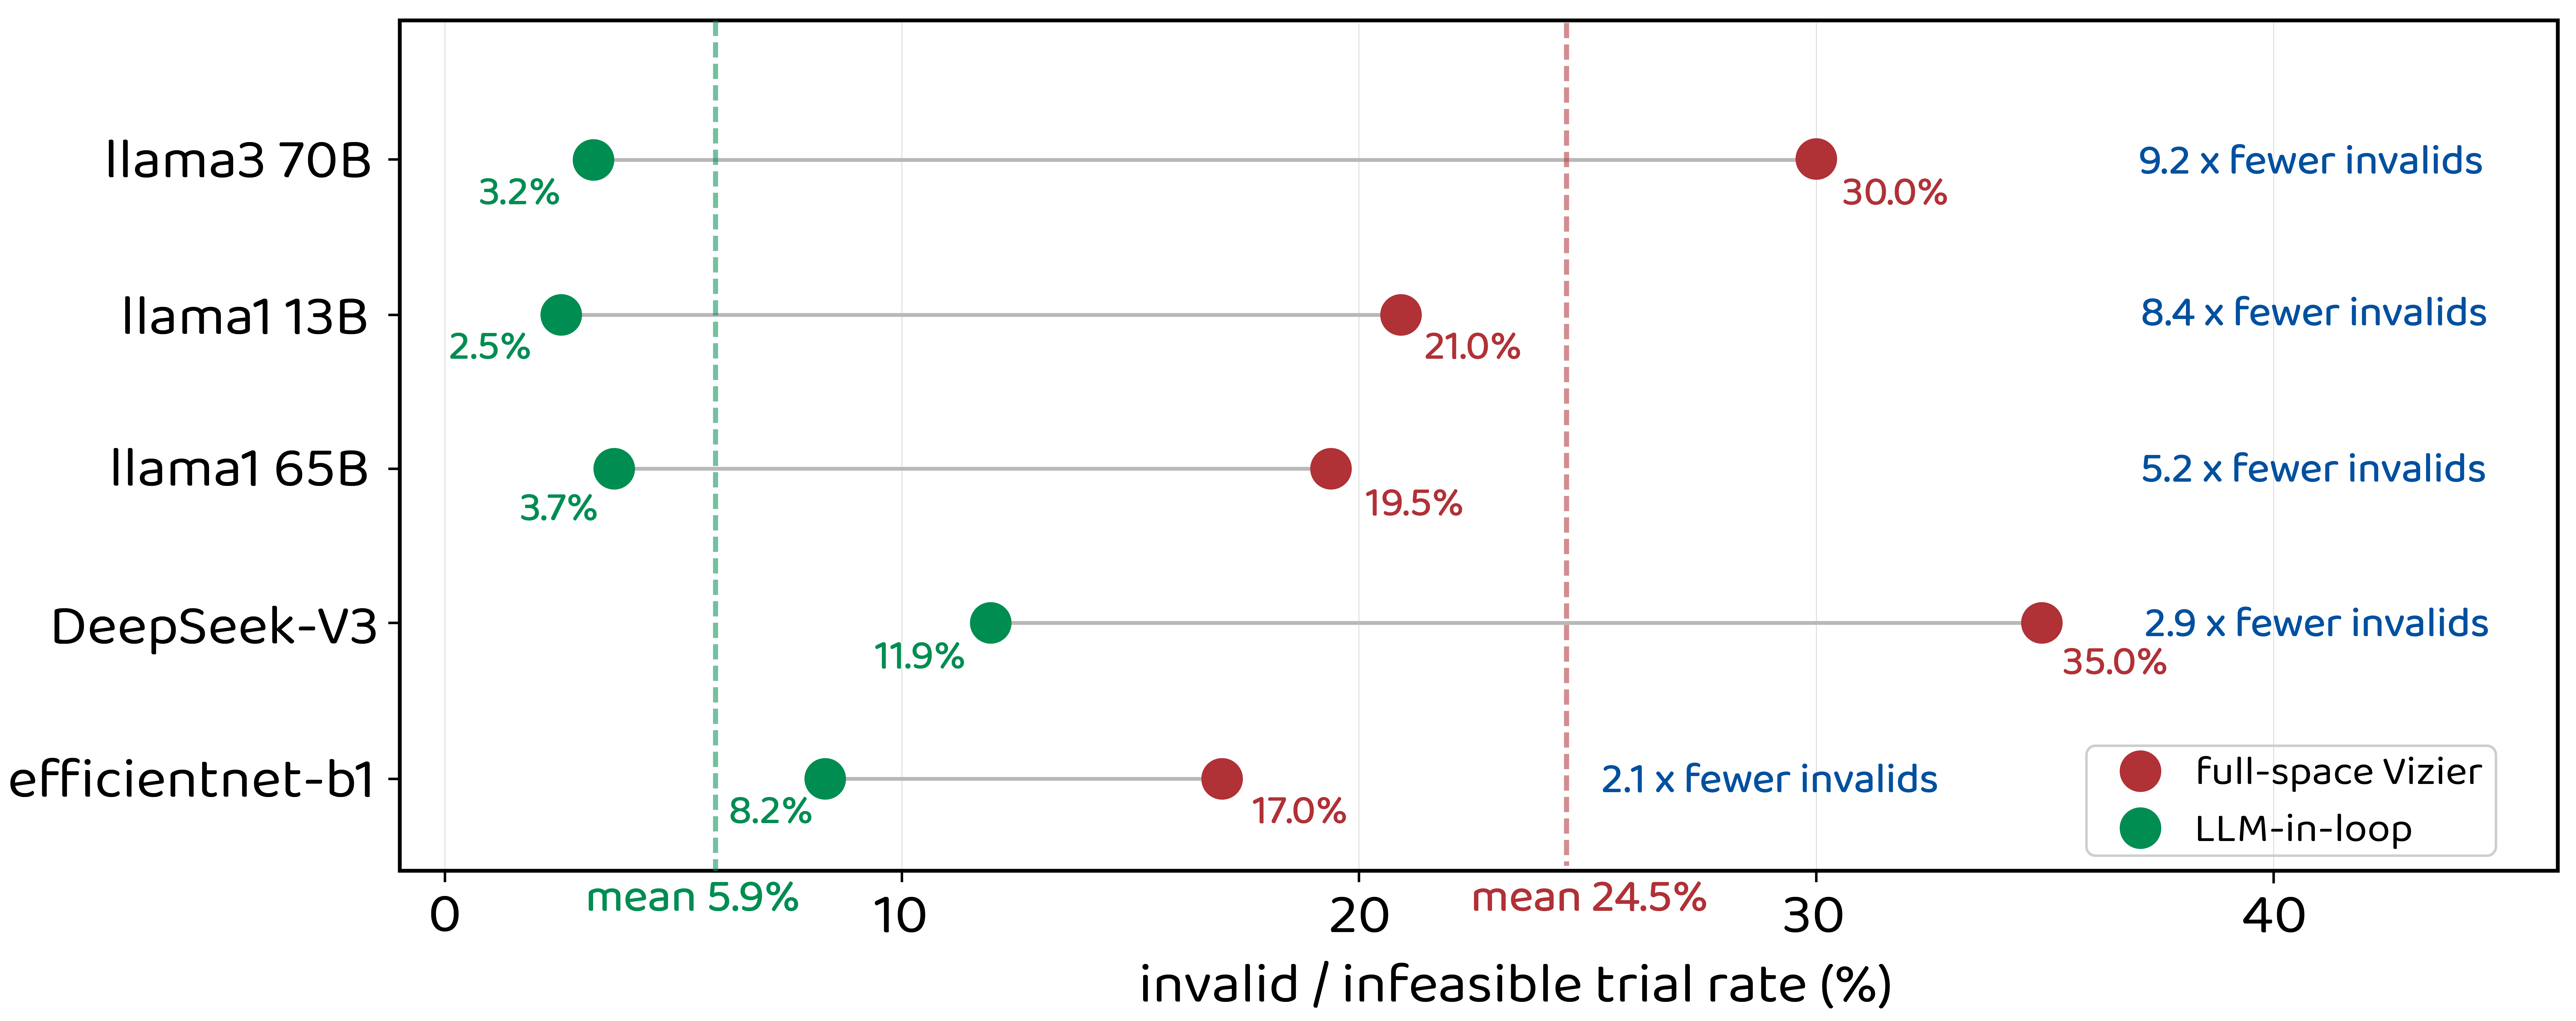
\includegraphics[width=0.48\textwidth]{fig3/llm_guide_v1.png}
% %     \caption{Strategic Intelligence vs.\ Stochastic Brute Force. Green indicates the LLM-Architect has less wasted trials.}
% %     \label{fig:llm}
% %     \vspace{-10pt}
% % \end{wrapfigure}

% % Modelled on SkyDiscovery~\citep{skydiscover2026}, the LLM Architect prunes
% % the outer search loop by proposing campaign patches rather than
% % predicting raw performance. It analyses a Causal Ledger containing
% % invalid rates, MFU, and solver diagnostics to suggest constrained
% % hardware neighbourhoods for Vizier to explore locally. The V1 LP
% % remains the ground-truth evaluator, supported by a Roofline Auditor
% % that rejects physically impossible results.
% % In a widened search space, the LLM loop reduces invalid evaluations
% % from $24.5\%$ to $5.9\%$ on average — a $4.1\times$ reduction in wasted
% % trials — while reaching the same optimal Perf/TDP scores as full-space
% % Vizier. This demonstrates that the LLM's role is steering Bayesian
% % optimisation toward feasible, workload-appropriate subspaces rather than
% % replacing the solver. This framework establishes a foundation for
% % integrating complex human reasoning into the co-design loop.

% % % \subsubsection{LLM Architect vs. Optimizer}
% % % The LLM Architect framework is modeled on SkyDiscover, and efficiently prunes the large outer hardware search loop by proposing campaign patches. Rather than predicting performance, the Architect reads a compact Causal Ledger containing invalid-rate history, MFU, roofline lower-bound checks, and LP diagnostics, then proposes a constrained hardware neighborhood for Vizier to search locally. The V1 LP remains the sole performance evaluator: for each candidate, it solves the joint tiling, fusion, placement, and rematerialization LP, while a deterministic Roofline Auditor rejects physically impossible results. In the widened V1 search space, all methods reach the same capped V1 Perf/TDP ceiling, so the key differentiator is search efficiency. The LLM loop reduces invalid hardware evaluations from 24.5\% under full-space Vizier to 5.9\% on average across five workloads, a 4.1× reduction in wasted trials, while preserving the same best V1 score. This shows that the LLM’s contribution is not replacing Vizier or the solver, but steering Bayesian optimization toward feasible, workload-appropriate architectural neighborhoods with far less wasted trials. This also sets the foundation for future work, where the LLM in the loop can adhere to follow more complex human reasoning signals.
% % % \begin{figure}[ht!]
% % %     \centering
% % % 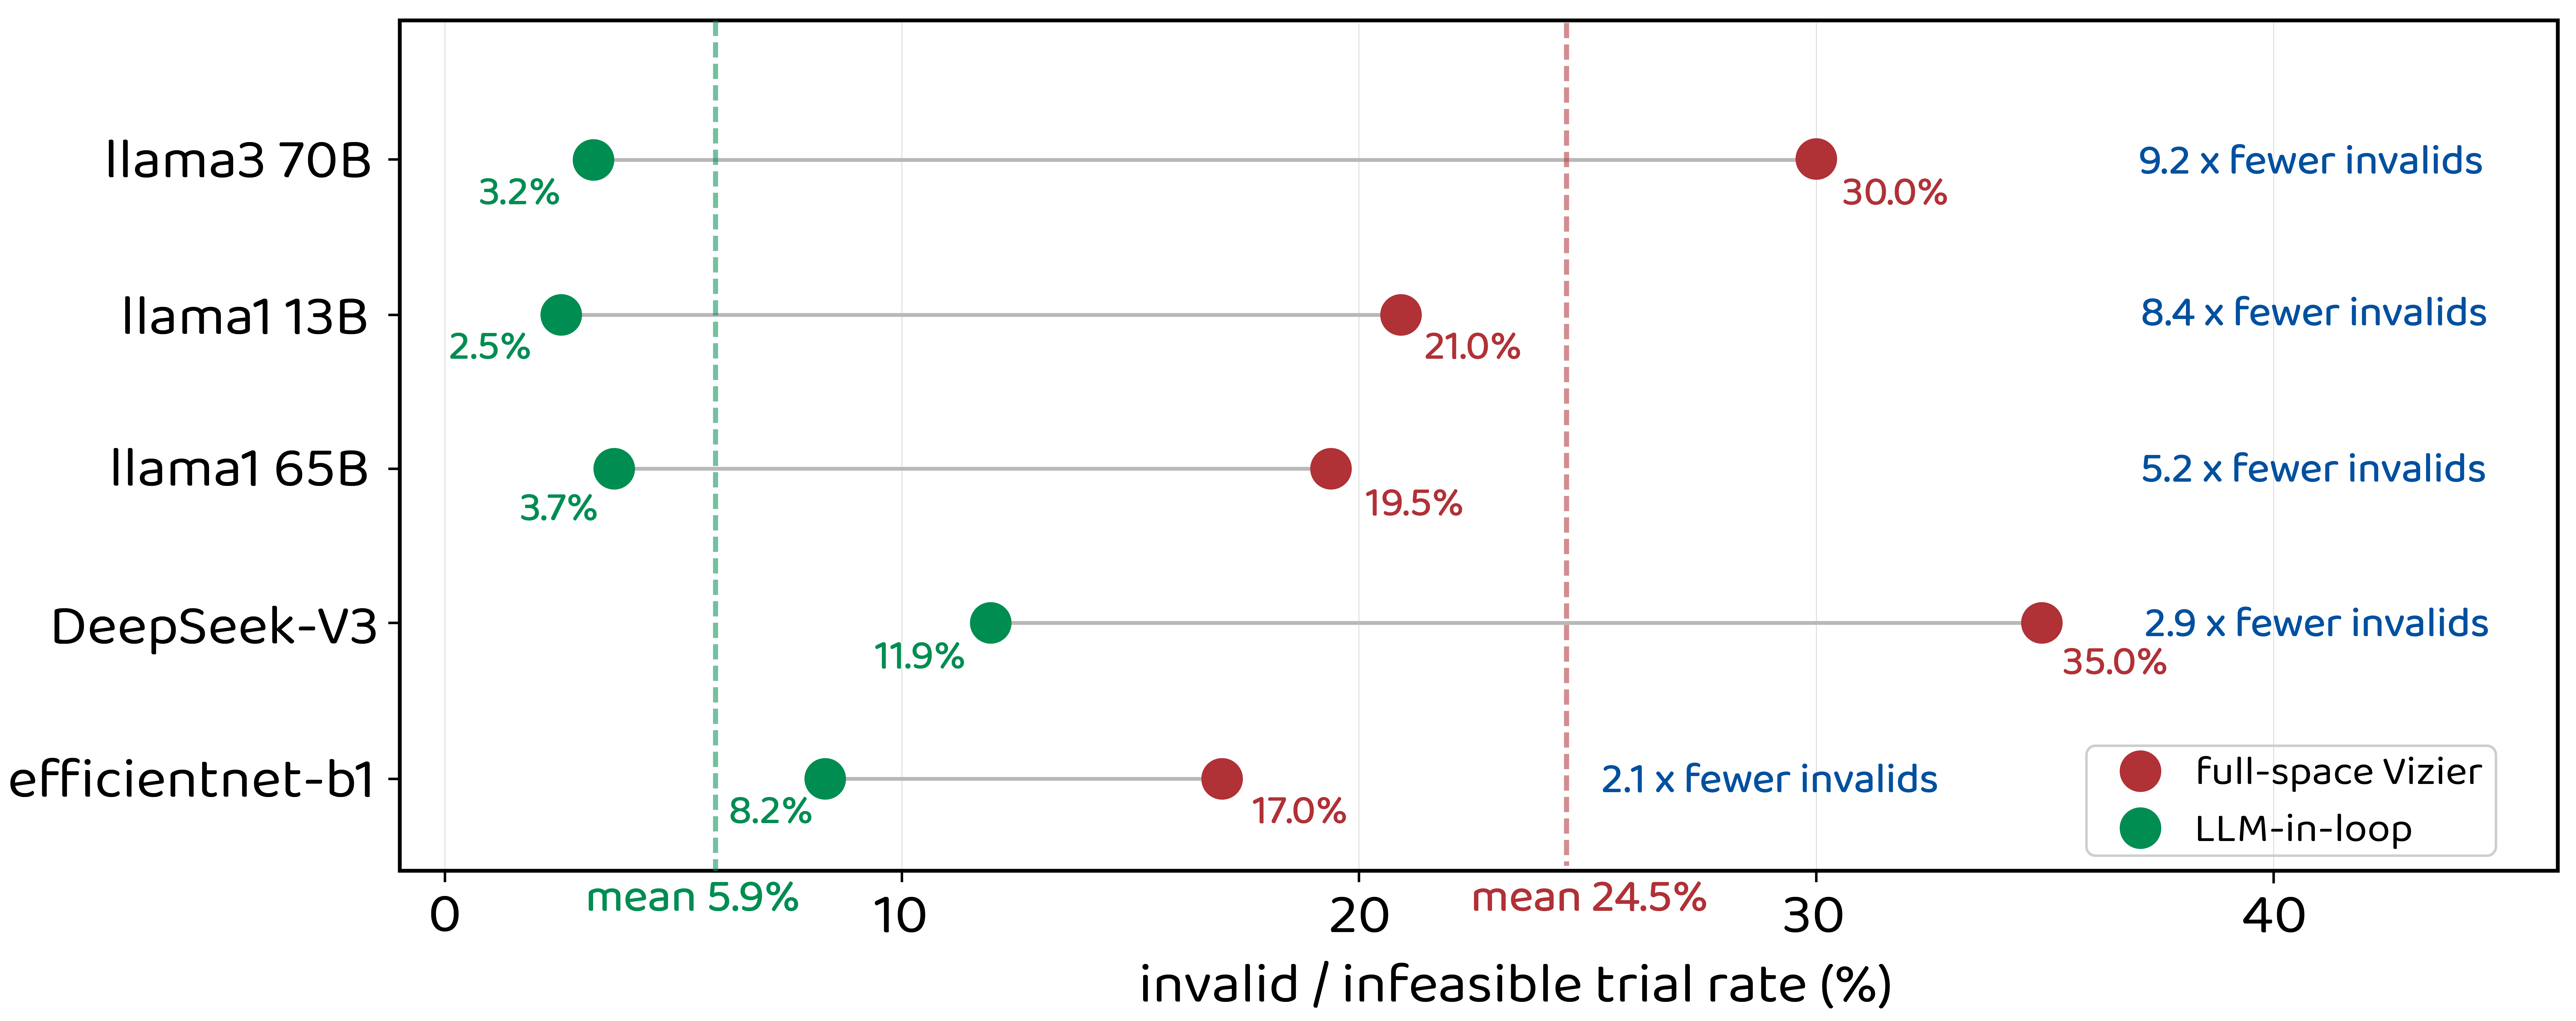
\includegraphics[width=0.85\linewidth]{fig3/llm_guide_v1.png}
% % % \caption{Strategic Intelligence vs. Stochastic Brute Force}\label{fig:llm}
% % % \end{figure}



% % % The LLM should not just ask, “What chip has the best Perf/TDP?” We aim to answer the question “Given this user’s workload and deployment goal, what is the architectural region to search for this deployment task?”. Therefore we have the LLM emit profile-conditioned campaigns that take specific user inference tasks into consideration. For each $(\text{deployment profile},\ \text{workload})$ cell, we ran a
% % % 200-trial LLM-Architect experiment using the same Qwen2.5-7B-Instruct + LoRA with differing user input profiles. At the start of each round, the prompt was assembled from a fixed system
% % % prompt, the active deployment profile, three few-shot examples, and a per-round user message containing the workload, recent feedback signals, current search bounds, and the causal ledger.
% % % The Strategist returned a one-line JSON campaign patch, which the
% % % validator accepted only if it was a strict legal subset of the parent space, satisfied hard rules such as patch-volume $\leq 10\%$, ridgepoint and MAC/BW constraints, and avoided forbidden regions.

% % % Thus, the experiment isolates whether the profile-conditioned LLM prompt alone can steer the same V1 evaluator toward different hardware families under different deployment intents.



% % % \todo{Compare convergence rate of LLM-guided hardware search vs.\ Vizier-only (Bayesian, LCS, random baselines) in the style of FAST Figure~11. Report:
% % % \begin{itemize}
% % %     \item Number of trials to reach $X\%$ of best Perf/TDP found by 5,000-trial Vizier
% % %     \item Quality of LLM-proposed configurations vs.\ Vizier-proposed configurations
% % %     \item Qualitative analysis of LLM reasoning about hardware bottlenecks
% % % \end{itemize}
% % % }

% % % \subsubsection{ROI Analysis}

% % % \todo{Update FAST's ROI analysis (Table~4) with the improved Perf/TDP numbers from FAST-CORGI. Report deployment volumes required to reach 1$\times$, 2$\times$, 4$\times$ ROI targets. If Perf/TDP improvements are larger than FAST's, the break-even deployment volume should decrease correspondingly.}

% % % \subsubsection{Pareto Frontier}

% % % \todo{Plot the Perf/TDP vs.\ area Pareto frontier for V1-optimized designs compared to FAST and TPU-v3 baseline, analogous to FAST Figure~12.}

% % page edit

% % \section{Experiments}
% % \label{sec:experiments}
% % In all cases we use an adapted JAX PDLP solver for large models at LLama70-B and DeepSeekv3 scale across all three methods (Static, CHEETAH-V0, CHEETAH-V1); and use HiGHS as the default solver for all other smaller neural network models. In order to be consistent with prior work, our experimental results are presented as orders of speedup / performance against a vanilla TPU-V3. This is also since TPUs are targeted for NN accelerators (as opposed to GPUs), and the TPU-V3 has the most information publically released, making it possible for us to simluate it more accurately. 

% % \subsection{Experimental Setup}

% % \paragraph{Static Sequential Baseline.}
% % We compare against the static optimization FAST framework using a simulated TPU-v3 baseline normalized to a sub-10nm process technology, following the same methodology as Zhang \etal. The baseline simulator is well-correlated with production hardware: on average within 8.2\,$\pm$\,2.7\% of profiled TPU-v3 performance. We evaluate against a \emph{simulated} TPU-v3 baseline to account for optimistic simulator assumptions.

% % We evaluate across 11 representative workloads: EfficientNet-B1 through EfficientNet-B7, Llama13, 65, 70 models, and DeepSeek-V3-MoE. These workloads stress different parts of the hardware design space: EfficientNet stresses low-operational-intensity depthwise convolutions, while Llama and DeepSeek stress memory capacity, bandwidth, and large matrix operations. 

% % \textbf{Single-workload specialization.} Each neural network workload is optimized independently. This experiment measures the best workload-specific hardware found under a fixed trial budget and identifies architectural preferences such as Global Memory size, bandwidth, MAC count, and systolic shape. In the case of Staitic and V0 methods, the pipeline involves: Vizier - Timeloop - LP solver. In the case of the V1 method, the pipeline is simplified to Vizier - LP solver. In each case we iterate for 100 trials per method x NN. 

% % % \textbf{Fixed-hardware-workload generalization.} We search for general-purpose datapaths that perform well across the workload suite. The objective is a harmonic or geometric aggregation of per-workload Perf/TDP, forcing the search to balance CNN-style memory pressure and LLM-style compute/memory trade-offs.

% % \textbf{LLM-Architect guides outer search.} We the LLM-guided outer-loop controller which proposes search-space interventions for Vizier. The advantage of the CHEETAH-V1 formulation is it removes dependence of Timeloop in the loop. Therefore the loop is reduced to just Vizier-LP solve, which dramatically speeds up the iterative process, thus permitting the LLM-Architect outer loop. The LLM is only permitted to change the search neighborhood of Vizier's input, the strict LP formulation on the inner loop does not change. This ensures mathematical and physical constraints are upheld in the space of co-design. 

% % % \paragraph{Optimization framework.}
% % % For the outer hardware search loop, we use Google Vizier with LCS optimization and safe search, running 100 trials per experiment (method X NN x Exp). Each trial invokes the LP solver for the inner optimization. The Static and V0 methods additionally have Timeloop in the loop (Vizier-Timeloop-LP solve). The advantage of the v1 formulation is it removes dependance of Timeloop in the loop. Therefore the loop is reduced to just Vizier-Lp solve, which dramatically speeds up the iterative process, thus permitted the Strategic LLM outer loop.

% % We validate our framework through a multi-level audit process to ensure physical and numerical rigor.
% % \textbf{Roofline Auditor.}
% % A deterministic Roofline Auditor enforces physical feasibility by
% % verifying that LP-predicted latencies never fall below the theoretical
% % bound
% % \begin{equation}
% %     \mathrm{LB} = \max\!\left(t_{\mathrm{compute}},\;
% %     t_{\mathrm{memory}}\right),
% %     \label{eq:roofline_lb_val}
% % \end{equation}
% % where $t_{\mathrm{compute}}$ and $t_{\mathrm{memory}}$ represent the
% % peak compute and memory bandwidth floors, respectively.
% % All reported V0/V1 results are roofline-feasible with valid
% % $\mathrm{MFU}_{\mathrm{bound}}$ and memory utilization metrics.

% % \textbf{Campaign Validator.}
% % A deterministic Campaign Validator legalizes LLM-proposed architectural
% % neighbourhoods by enforcing hard hardware constraints — including TDP
% % caps, area limits, and power-of-two parameter ranges — prior to Vizier
% % sampling.

% % \textbf{Causal Ledger.}
% % A Causal Ledger tracks LLM interventions and observed outcomes,
% % preventing redundant exploration of empirically invalid regions and
% % ensuring full auditability of the search loop.

% % \textbf{Solver Diagnostics.}
% % We monitor solver diagnostics including primal/dual residuals, duality
% % gap, and rounding gap. Designs are treated as trustworthy only when both
% % the continuous LP relaxation and the rounded integer solution are
% % numerically well-behaved.


% % \subsection{Main Results}

% % % \subsubsection{V0 vs.\ FAST Static Fusion}

% % % \todo{Insert results table and figure comparing V0 (time-indexed placement + rematerialization) against FAST's static fusion ILP on all benchmarks. Key metrics: Perf/TDP improvement, fusion efficiency (\% of DRAM stall time eliminated), rematerialization frequency (how often does the solver choose to recompute rather than reload?).}

% % % \paragraph{Expected findings.}
% % % V0's dynamic placement should show the largest gains on workloads with: (1)~tight Global Memory budgets where static pinning wastes capacity on tensors that are only needed briefly, (2)~long dependency chains where tensor lifetimes vary substantially, and (3)~cheap-to-recompute operations with large activations (\eg, depthwise convolutions in EfficientNet).

% % % \subsubsection{V1 vs.\ V0: Joint Tiling and Fusion}

% % % \todo{Insert results table and figure comparing V1 against V0 on all benchmarks. Key metrics: Perf/TDP improvement, number of operations where V1 selects a different tiling configuration than Timeloop's greedy choice, and the resulting compute efficiency vs.\ fusion trade-off.}

% % % \paragraph{Expected findings.}
% % % V1 should show the largest gains on architectures with highly diverse layer types where a single tiling configuration cannot serve all operations well. EfficientNet (depthwise + pointwise convolutions with 100$\times$ variation in working-set sizes) and hybrid CNN-transformer models (convolutions + attention + MLP with fundamentally different compute-memory profiles) are expected to benefit most.


% % % \subsubsection{stiatic vs v0 vs v1}
% % % \begin{figure}[ht!]
% % %     \centering
% % %     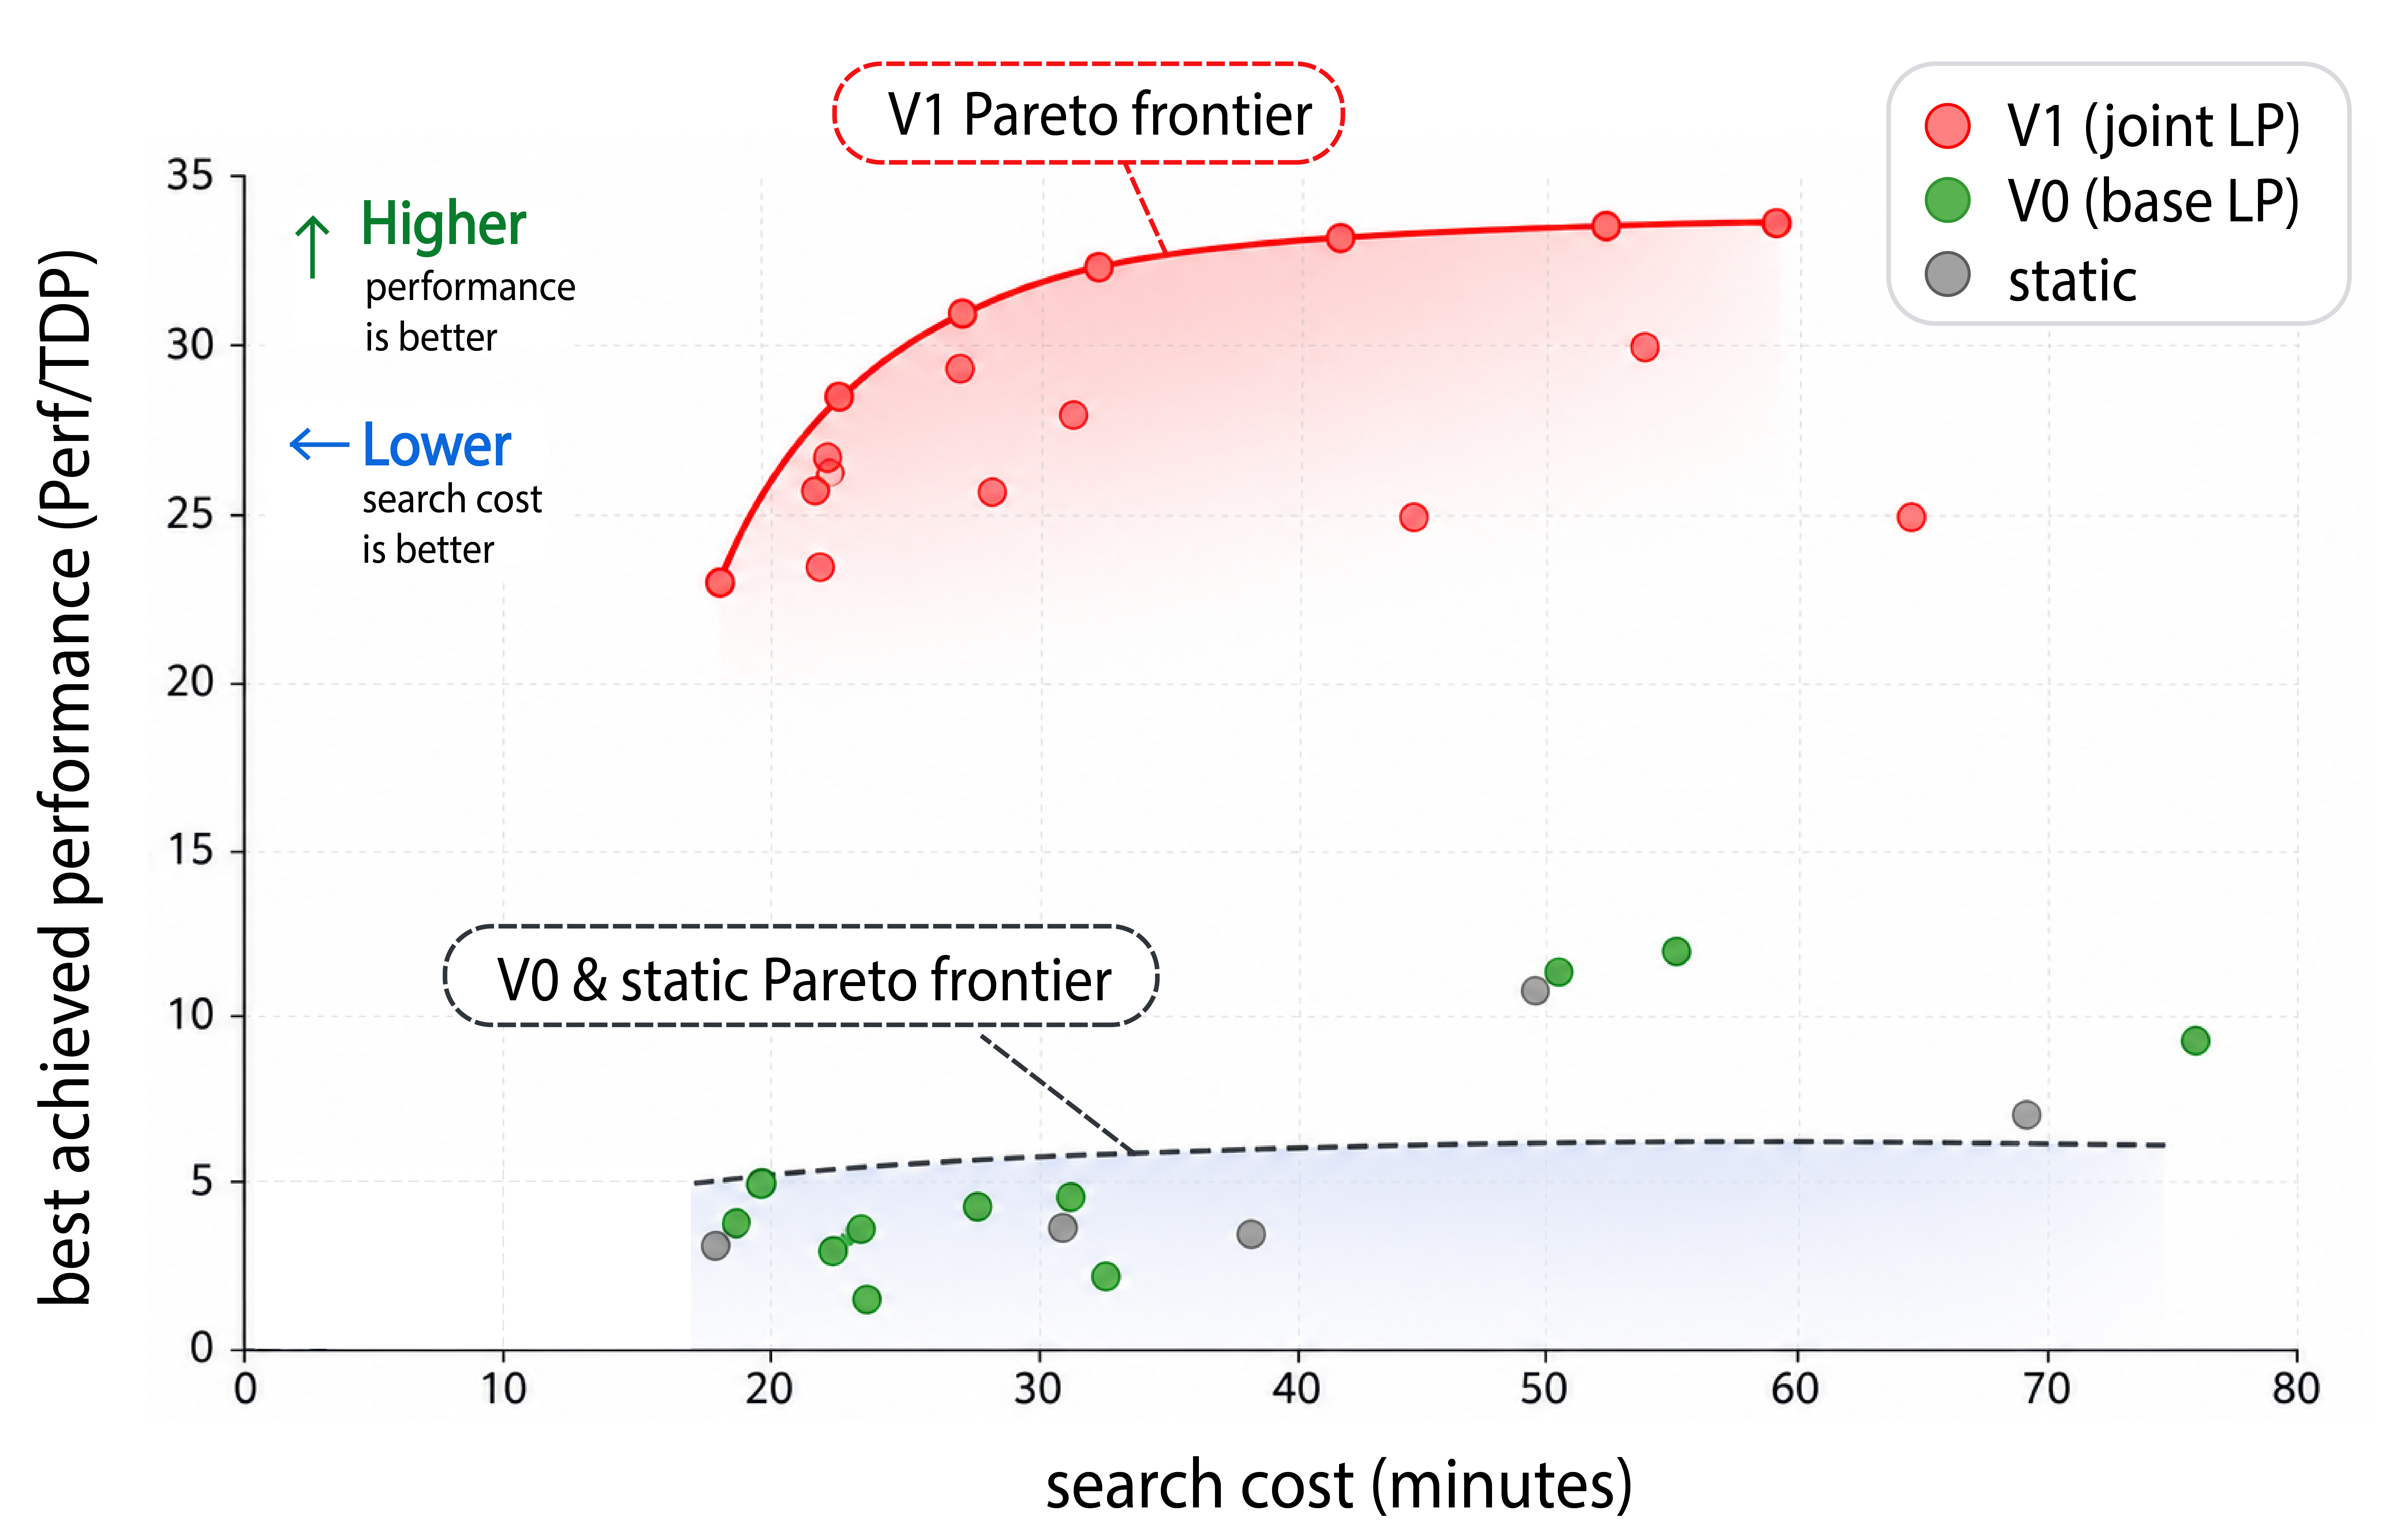
\includegraphics[width=0.7\linewidth]{figs/pareto_v2.png}
% % %     \caption{pareto frontier plot}
% % % \end{figure}
% % \begin{figure}[ht!]
% %     \centering
% % 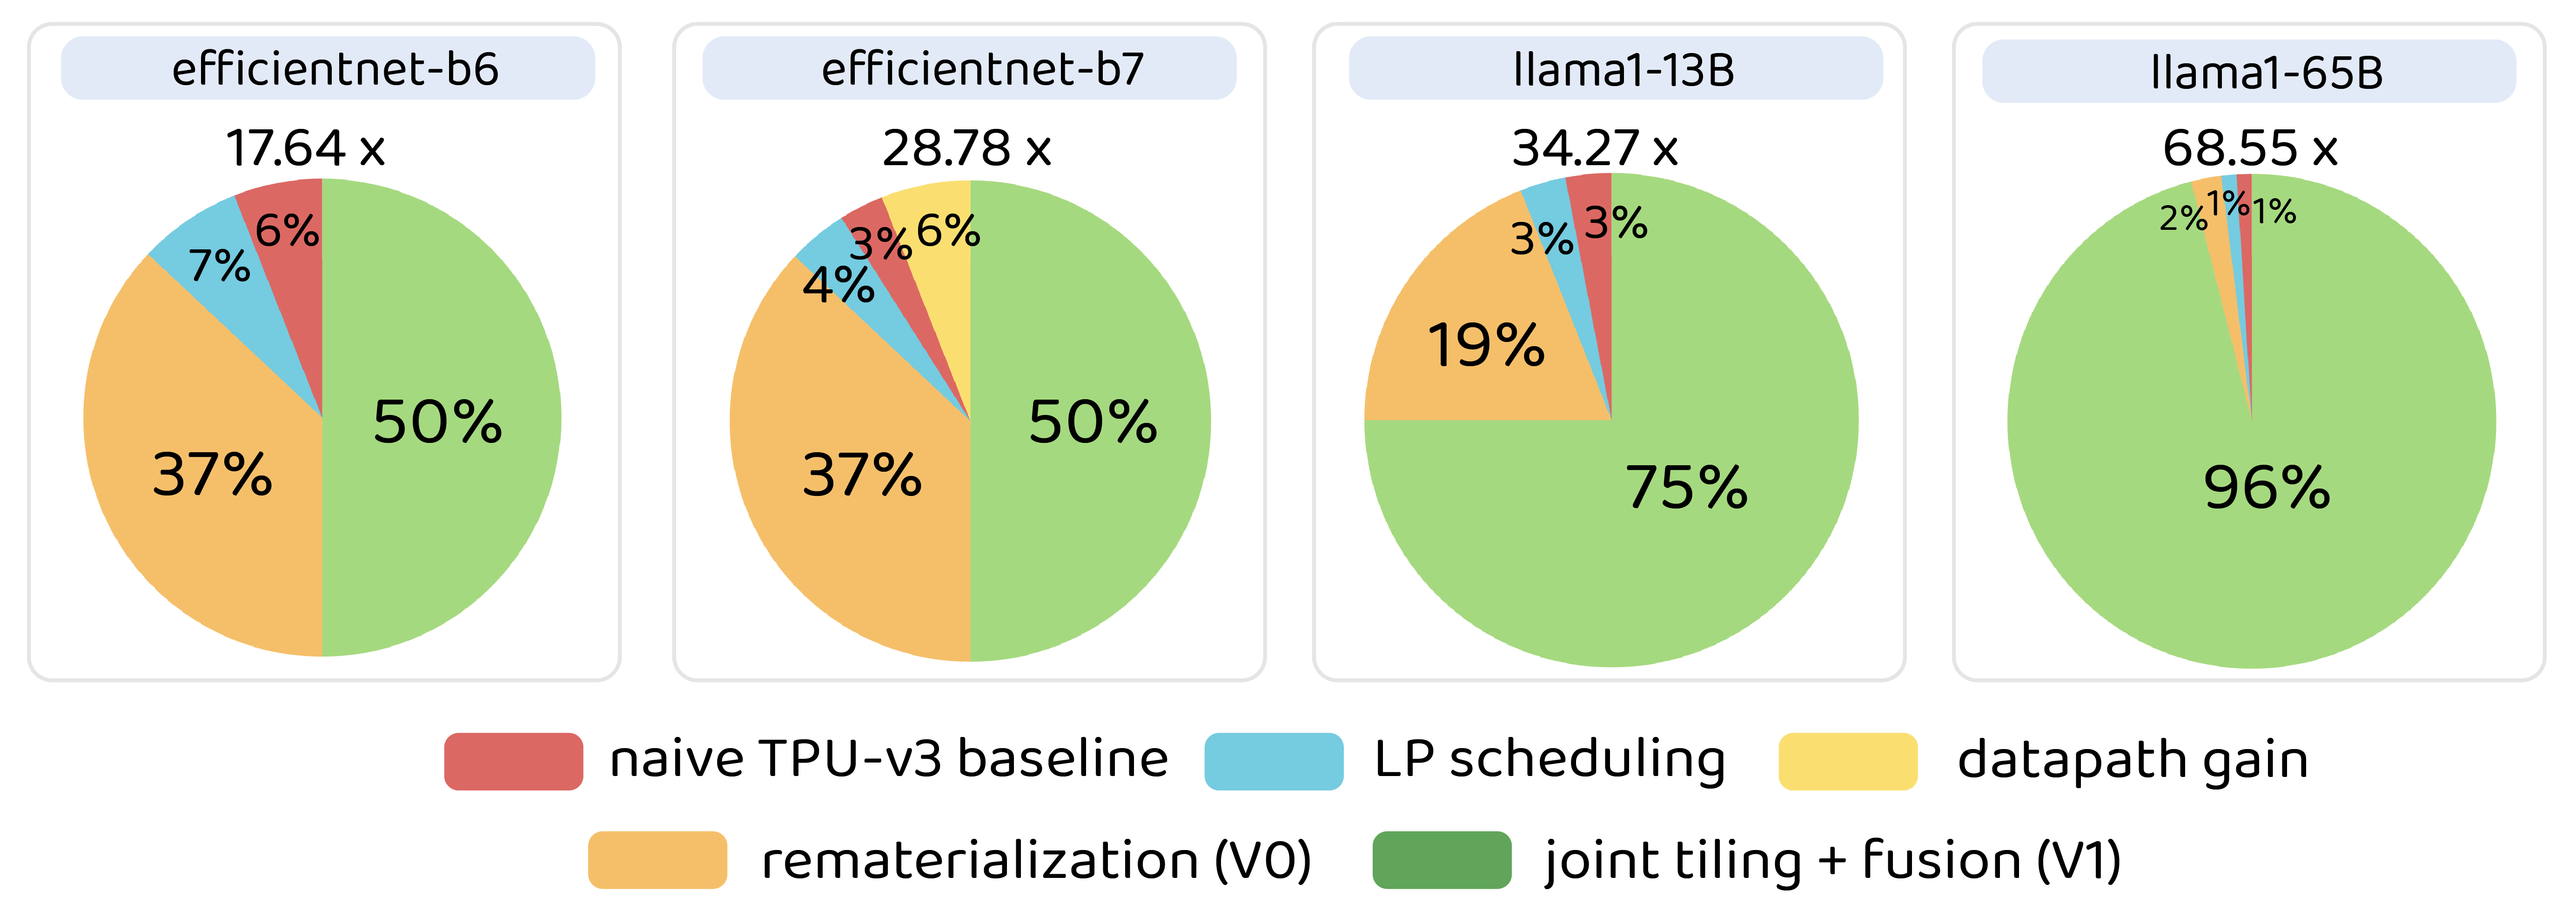
\includegraphics[width=0.85\linewidth]{fig3/speedup_decomposition_final_v2.png}
% % \caption{Speedup decomposition over naive TPU-v3 baseline. Each pie shows the 
% % relative contribution of four optimization sources to the total speedup. CHEETAH-V1 joint tiling + fusion dominates on all workloads, 
% % especially on larger models where memory management is the primary bottleneck.}\label{fig:accel_decompose}
% % \end{figure}
% % \subsubsection{Static Baseline vs.\ CHEETAH-V0 vs.\ CHEETAH-V1 Unlock Progressive Gains}


% % Figure~\ref{fig:accel_decompose} decomposes the total speedup over a naive TPU-v3 baseline into four sources: LP-based scheduling and fusion, datapath gain from hardware search, dynamic rematerialization (CHEETAH-V0), and joint tiling + fusion (CHEETAH-V1).

% % The dominant contributor across all workloads is V1's joint tiling-fusion 
% % optimization. On EfficientNet-B1, V1 accounts for 50\% of total speedup, 
% % with LP scheduling (28\%) and datapath gain (22\%) splitting the remainder---and 
% % no rematerialization benefit, consistent with B1's small activation footprint 
% % fitting comfortably in Global Memory. B3--B4 show a similar 50\% V1 share, but 
% % V0 rematerialization now contributes 25\%, reflecting the growing value of 
% % recomputing large depthwise activations rather than reloading them from DRAM. 
% % From B5 onward, V1's share rises sharply to 75--88\%, as the increasing 
% % model size makes joint tiling-fusion the primary lever: memory management 
% % dominates, and the remaining sources (LP scheduling, V0, datapath) each shrink 
% % to single-digit percentages. The same pattern holds on Llama, where V1 accounts 
% % for 83--87\% of the total speedup.

% % % \begin{wrapfigure}{r}{0.48\textwidth}
% % %     \centering
% % %     \vspace{-12pt}
% % %     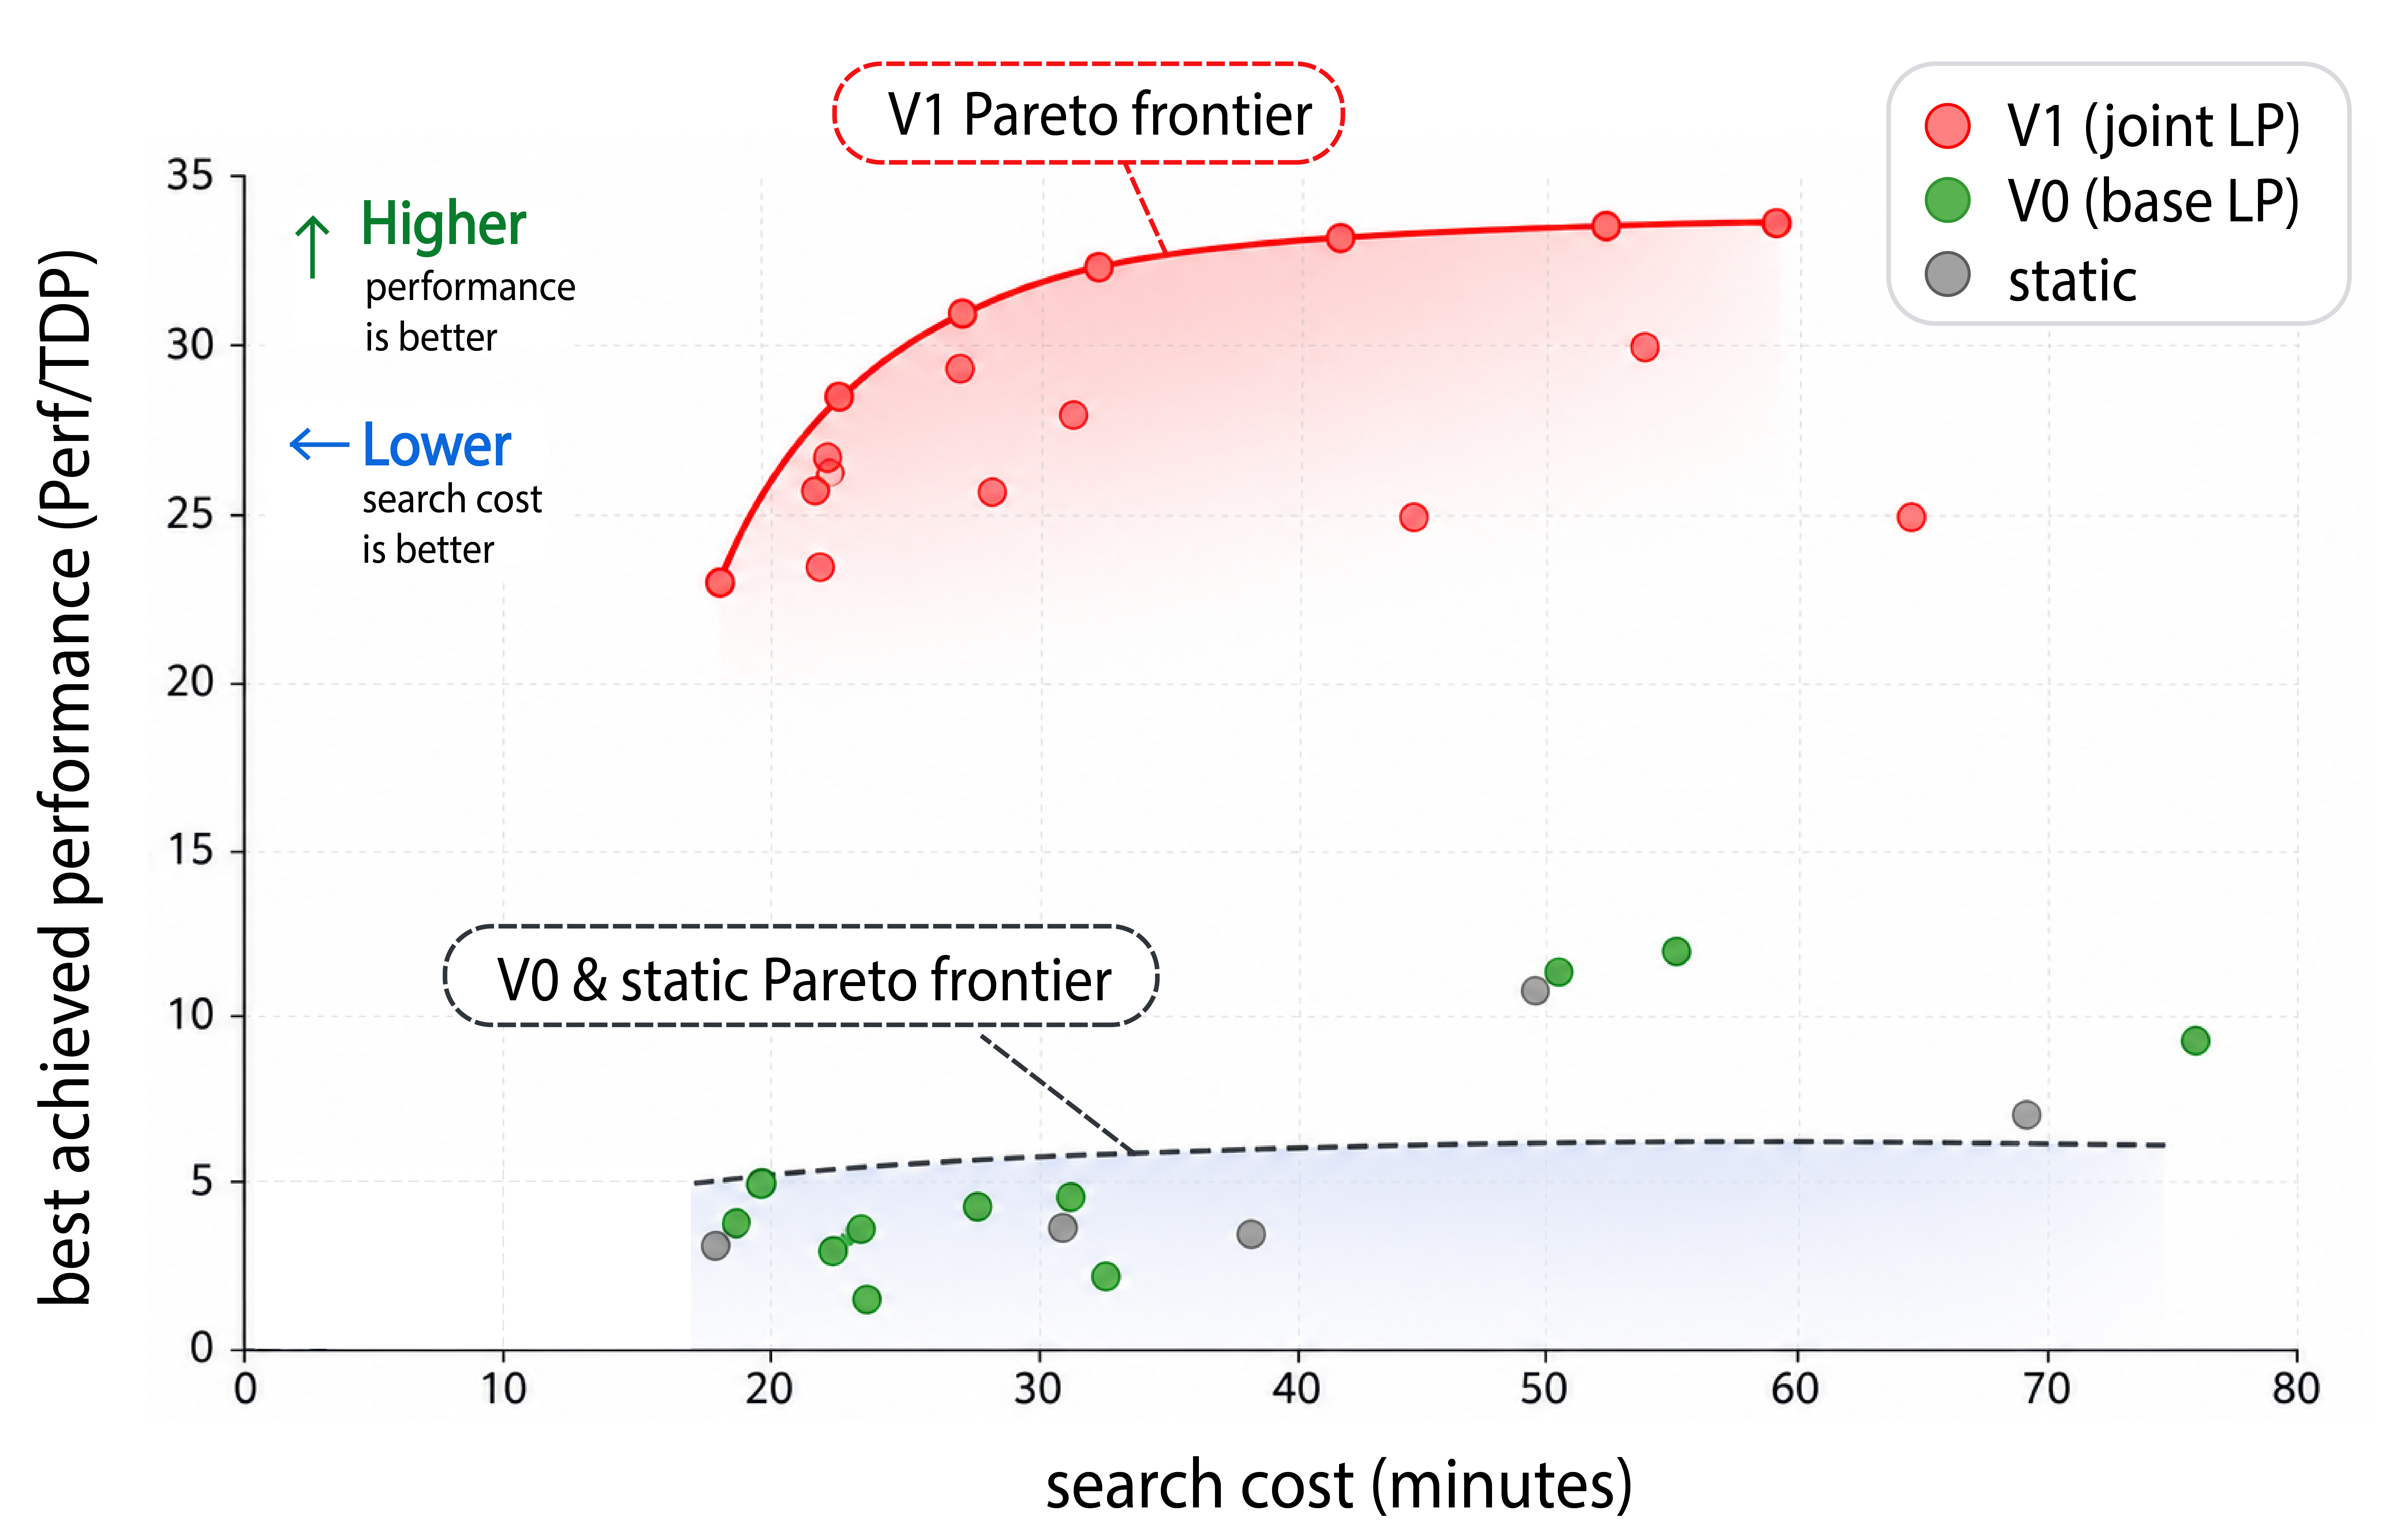
\includegraphics[width=0.48\textwidth]{figs/pareto_v2.png}
% % %     \vspace{-18pt}
% % %     \caption{Search cost vs.\ Perf/TDP Pareto frontier. V1 dominates V0 and static across all time budgets.}
% % %     \label{fig:pareto}
% % %     \vspace{-10pt}
% % % \end{wrapfigure}

% % Critically, Figure~\ref{fig:speedup} shows static fusion method is \emph{infeasible} on modern large models (Llama-70B, and DeepSeek-V3), because their large activation tensors cannot fit under a static pinning policy. The V0 formulation resolves feasibility for on large models via dynamic placement but remains time-intensive for a small number of 50 trials: measuring 58.42 hours on Llama-70B and 69.39 hours on DeepSeek-V3 (Figure~\ref{fig:wallclock}). In contrast Figures~\ref{fig:wallclock} and ~\ref{fig:speedup}, show the CHEETAH-V1 formulation out performs comparitive strategies in terms of speedup against the TPU-V3 baseline, and require only 1.17 hours on Llama-70B and 2.17 hours on DeepSeekv3 for 50 trails---a ${\sim}93\%$ average reduction. The powerful joint formulation is able to select memory-efficient tiling configurations alongside placement, achieving feasibility across the entire workload suite, demonstrating that joint optimization is not merely an incremental improvement but a qualitative capability unlock for large-scale models.

% % % This demonstrates that by exploiting structural invariance and GPU-accelerated mathematical optimization, CHEETAH-V1 reduces the end-to-end co-design search time from days to under 2.2 hours—a ${\sim}93\%$ average reduction—while discovering architectural points that deliver up to $35\times$ speedup over the TPU-v3 baseline.

% % % Figure~\ref{fig:pareto} shows the Pareto frontier of best-achieved Perf/TDP versus wall-clock search cost. V1 strictly dominates both V0 and static at every time budget: within 10 minutes of search, V1 already exceeds the best Perf/TDP that V0 or static achieve after 60+ minutes. The V1 Pareto frontier reaches ${\sim}35\times$ Perf/TDP, roughly $3\times$ higher than the V0/static frontier at ${\sim}10\text{--}12\times$. This gap reflects two compounding advantages: V1 explores a strictly larger feasible region (joint tiling-fusion), and it eliminates Timeloop from the per-trial critical path, allowing more trials within any fixed time budget.



% % \paragraph{Practical insight.}
% % Both LPs are extreme-aspect-ratio sparse: for \texttt{llama3\_70b},
% % $m, n \sim 10^6$ and $\mathrm{nnz} \sim 5 \times 10^6$, giving roughly
% % 1 nonzero per million matrix entries.
% % The time-band structure means a coordinate-descent or stochastic PDHG
% % solver would converge in $\mathcal{O}(T)$ sweeps if bands were the only
% % structure.
% % The capacity rows in both V0 and V1 LP formulations are the sole feature breaking strict banded structure, and they are precisely what couples the schedule globally. This is the desired behavior of a memory-aware placement formulation.

% % % \todo{Report LP solve times for V0 and V1 across all benchmarks. Compare wall-clock time per trial against FAST's SCIP-based ILP solver (20 min timeout). Report LP relaxation gap: how often do fractional solutions need integer rounding, and what is the quality loss from rounding?}

% % \paragraph{Structural invariance.}
% % For a fixed workload and LP formulation, the LP constraint matrix
% % has an invariant sparsity pattern across trials: the row/column
% % dimensions and nonzero locations are determined only by the model graph structure — layer count $L$, timestep count $T$, edge set $E$, and Pareto count $C$ — not by the hardware candidate.
% % Vizier changes only numerical values such as cycle coefficients,
% % memory-capacity bounds, bandwidth-scaled access costs, objective weights, and TDP/area parameters. 
% % This invariance allows us to reuse the same sparse matrix structure,
% % variable ordering, block layout, and JIT-compiled sparse kernels in our adapted JAX PDLP solver across all hardware trials for a given workload.

% % Numerically, we apply the same diagonal preconditioning pipeline
% % on each trial: a structural presolve with 20 log-geomean Ruiz iterations, followed by the PDLP preprocessing stack with 10 infinity-norm Ruiz iterations and one Pock--Chambolle $\ell_1$-scaling pass. This two-stage diagonal scaling handles the mixed coefficient magnitudes present in V0/V1 matrices — large byte-valued capacity rows together with $\pm 1$ persistence rows — without requiring a fragile matrix factorization.

% % In production, this preconditioning pipeline is reused structurally across trials, recomputes only cheap diagonal scalings, finishes in under one second for matrices with approximately $5 \times 10^6$ nonzeros, and avoids factorization failures entirely because it consists only of $D_1 A D_2$ arithmetic.

% % \subsubsection{LLM Architect vs. Optimizer}
% % The LLM Architect framework is modeled on SkyDiscover, and efficiently prunes the large outer hardware search loop by proposing campaign patches. Rather than predicting performance, the Architect reads a compact Causal Ledger containing invalid-rate history, MFU, roofline lower-bound checks, and LP diagnostics, then proposes a constrained hardware neighborhood for Vizier to search locally. The V1 LP remains the sole performance evaluator: for each candidate, it solves the joint tiling, fusion, placement, and rematerialization LP, while a deterministic Roofline Auditor rejects physically impossible results. In the widened V1 search space, all methods reach the same capped V1 Perf/TDP ceiling, so the key differentiator is search efficiency. The LLM loop reduces invalid hardware evaluations from 24.5\% under full-space Vizier to 5.9\% on average across five workloads, a 4.1× reduction in wasted trials, while preserving the same best V1 score. This shows that the LLM’s contribution is not replacing Vizier or the solver, but steering Bayesian optimization toward feasible, workload-appropriate architectural neighborhoods with far less wasted trials. This also sets the foundation for future work, where the LLM in the loop can adhere to follow more complex human reasoning signals.
% % \begin{figure}[ht!]
% %     \centering
% % 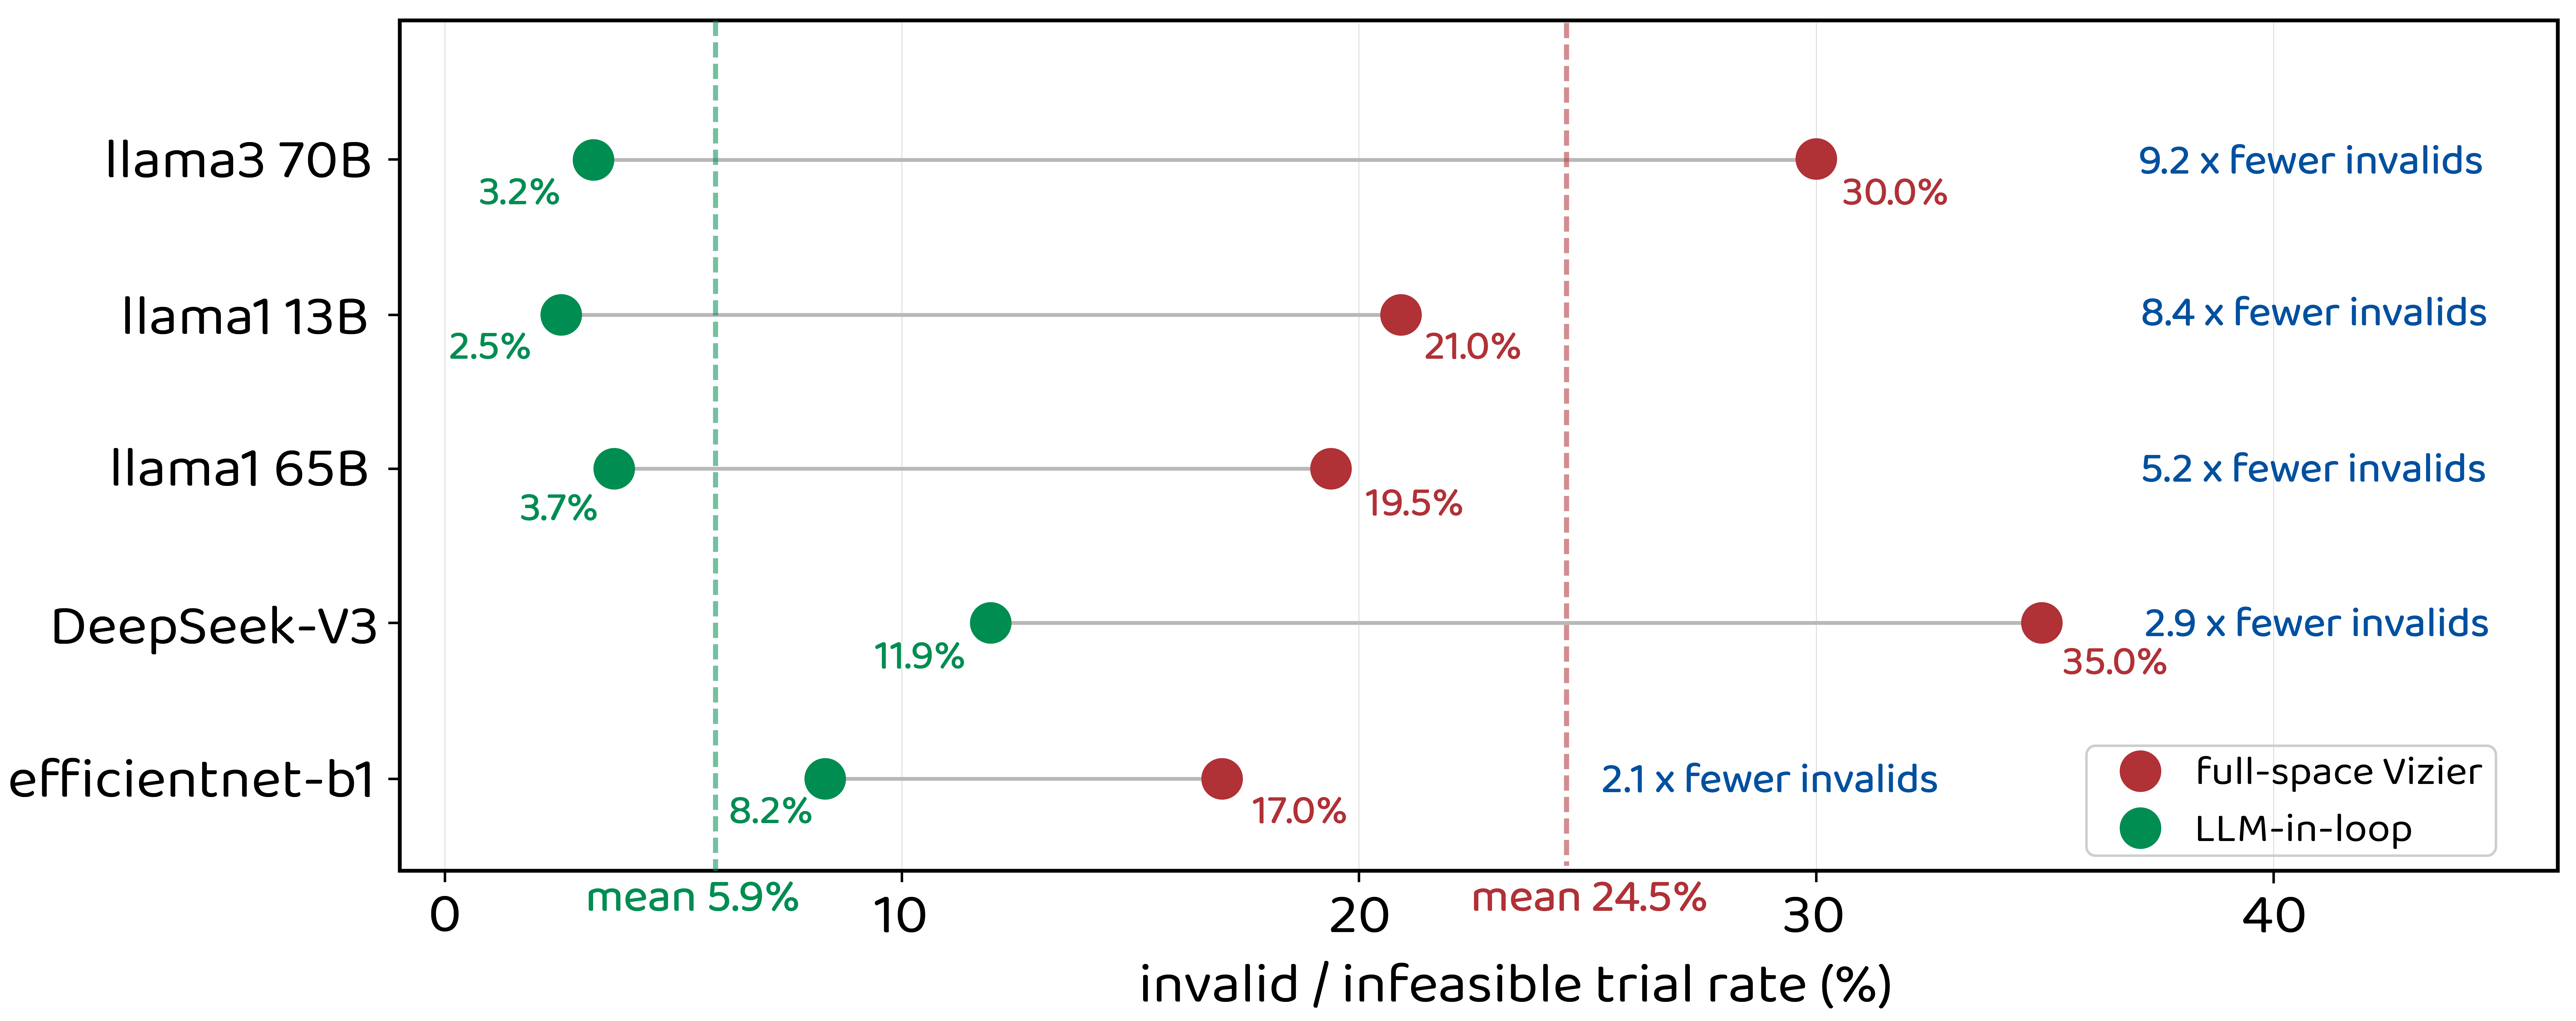
\includegraphics[width=0.85\linewidth]{fig3/llm_guide_v1.png}
% % \caption{Strategic Intelligence vs. Stochastic Brute Force}\label{fig:llm}
% % \end{figure}



% % % The LLM should not just ask, “What chip has the best Perf/TDP?” We aim to answer the question “Given this user’s workload and deployment goal, what is the architectural region to search for this deployment task?”. Therefore we have the LLM emit profile-conditioned campaigns that take specific user inference tasks into consideration. For each $(\text{deployment profile},\ \text{workload})$ cell, we ran a
% % % 200-trial LLM-Architect experiment using the same Qwen2.5-7B-Instruct + LoRA with differing user input profiles. At the start of each round, the prompt was assembled from a fixed system
% % % prompt, the active deployment profile, three few-shot examples, and a per-round user message containing the workload, recent feedback signals, current search bounds, and the causal ledger.
% % % The Strategist returned a one-line JSON campaign patch, which the
% % % validator accepted only if it was a strict legal subset of the parent space, satisfied hard rules such as patch-volume $\leq 10\%$, ridgepoint and MAC/BW constraints, and avoided forbidden regions.

% % % Thus, the experiment isolates whether the profile-conditioned LLM prompt alone can steer the same V1 evaluator toward different hardware families under different deployment intents.



% % % \todo{Compare convergence rate of LLM-guided hardware search vs.\ Vizier-only (Bayesian, LCS, random baselines) in the style of FAST Figure~11. Report:
% % % \begin{itemize}
% % %     \item Number of trials to reach $X\%$ of best Perf/TDP found by 5,000-trial Vizier
% % %     \item Quality of LLM-proposed configurations vs.\ Vizier-proposed configurations
% % %     \item Qualitative analysis of LLM reasoning about hardware bottlenecks
% % % \end{itemize}
% % % }

% % % \subsubsection{ROI Analysis}

% % % \todo{Update FAST's ROI analysis (Table~4) with the improved Perf/TDP numbers from FAST-CORGI. Report deployment volumes required to reach 1$\times$, 2$\times$, 4$\times$ ROI targets. If Perf/TDP improvements are larger than FAST's, the break-even deployment volume should decrease correspondingly.}

% % % \subsubsection{Pareto Frontier}

% % % \todo{Plot the Perf/TDP vs.\ area Pareto frontier for V1-optimized designs compared to FAST and TPU-v3 baseline, analogous to FAST Figure~12.}


% % edit for page limit
% \vspace{-0.3cm}
% \section{Experiments}
% \label{sec:experiments}
% \vspace{-0.2cm}
% \subsection{Experimental Setup}
% \vspace{-0.2cm}
% We compare against the FAST framework~\citep{zhang_fast} using a simulated TPU-v3 \citep{jouppi2021ten} baseline normalized to sub-10nm process technology (within $8.2 \pm 2.7\%$ of profiled TPU-v3 performance). We use an adapted JAX PDLP solver for large models (Llama-70B, DeepSeek-V3) and HiGHS \citep{huangfu2018parallel} for smaller models, reporting speedup over the TPU-v3 baseline consistent with prior work.
% We evaluate across 11 workloads: EfficientNet-B1 \citep{tan2019efficientnet} through B7 (stressing low-intensity depthwise convolutions), Llama-1 13B/65B and Llama-3 70B \citep{llama3modelcard}, and DeepSeek-V3-MoE \citep{deepseekv3report} (stressing memory capacity and bandwidth). Each workload is optimized independently under 100 trials per method. For Static and V0, the pipeline is Vizier$\to$Timeloop$\to$LP; for V1, it simplifies to Vizier$\to$LP. The LLM Architect outer loop proposes search-space interventions for Vizier; it is only permitted to change Vizier's search neighborhood while the strict LP inner loop remains unchanged.
% We validate all results through a multi-level audit process---Roofline Auditor, Campaign Validator, Causal Ledger, and solver diagnostics---as described in Section~\ref{sec:llm_outer} and detailed in Appendix~\ref{app:validation} and ~\ref{app:mfu}. All reported V0/V1 results are roofline-feasible with zero lower-bound violations.


% % \subsection{Main Results}

% % \subsubsection{V0 vs.\ FAST Static Fusion}

% % \todo{Insert results table and figure comparing V0 (time-indexed placement + rematerialization) against FAST's static fusion ILP on all benchmarks. Key metrics: Perf/TDP improvement, fusion efficiency (\% of DRAM stall time eliminated), rematerialization frequency (how often does the solver choose to recompute rather than reload?).}

% % \paragraph{Expected findings.}
% % V0's dynamic placement should show the largest gains on workloads with: (1)~tight Global Memory budgets where static pinning wastes capacity on tensors that are only needed briefly, (2)~long dependency chains where tensor lifetimes vary substantially, and (3)~cheap-to-recompute operations with large activations (\eg, depthwise convolutions in EfficientNet).

% % \subsubsection{V1 vs.\ V0: Joint Tiling and Fusion}

% % \todo{Insert results table and figure comparing V1 against V0 on all benchmarks. Key metrics: Perf/TDP improvement, number of operations where V1 selects a different tiling configuration than Timeloop's greedy choice, and the resulting compute efficiency vs.\ fusion trade-off.}

% % \paragraph{Expected findings.}
% % V1 should show the largest gains on architectures with highly diverse layer types where a single tiling configuration cannot serve all operations well. EfficientNet (depthwise + pointwise convolutions with 100$\times$ variation in working-set sizes) and hybrid CNN-transformer models (convolutions + attention + MLP with fundamentally different compute-memory profiles) are expected to benefit most.


% % \subsubsection{stiatic vs v0 vs v1}
% % \begin{figure}[ht!]
% %     \centering
% %     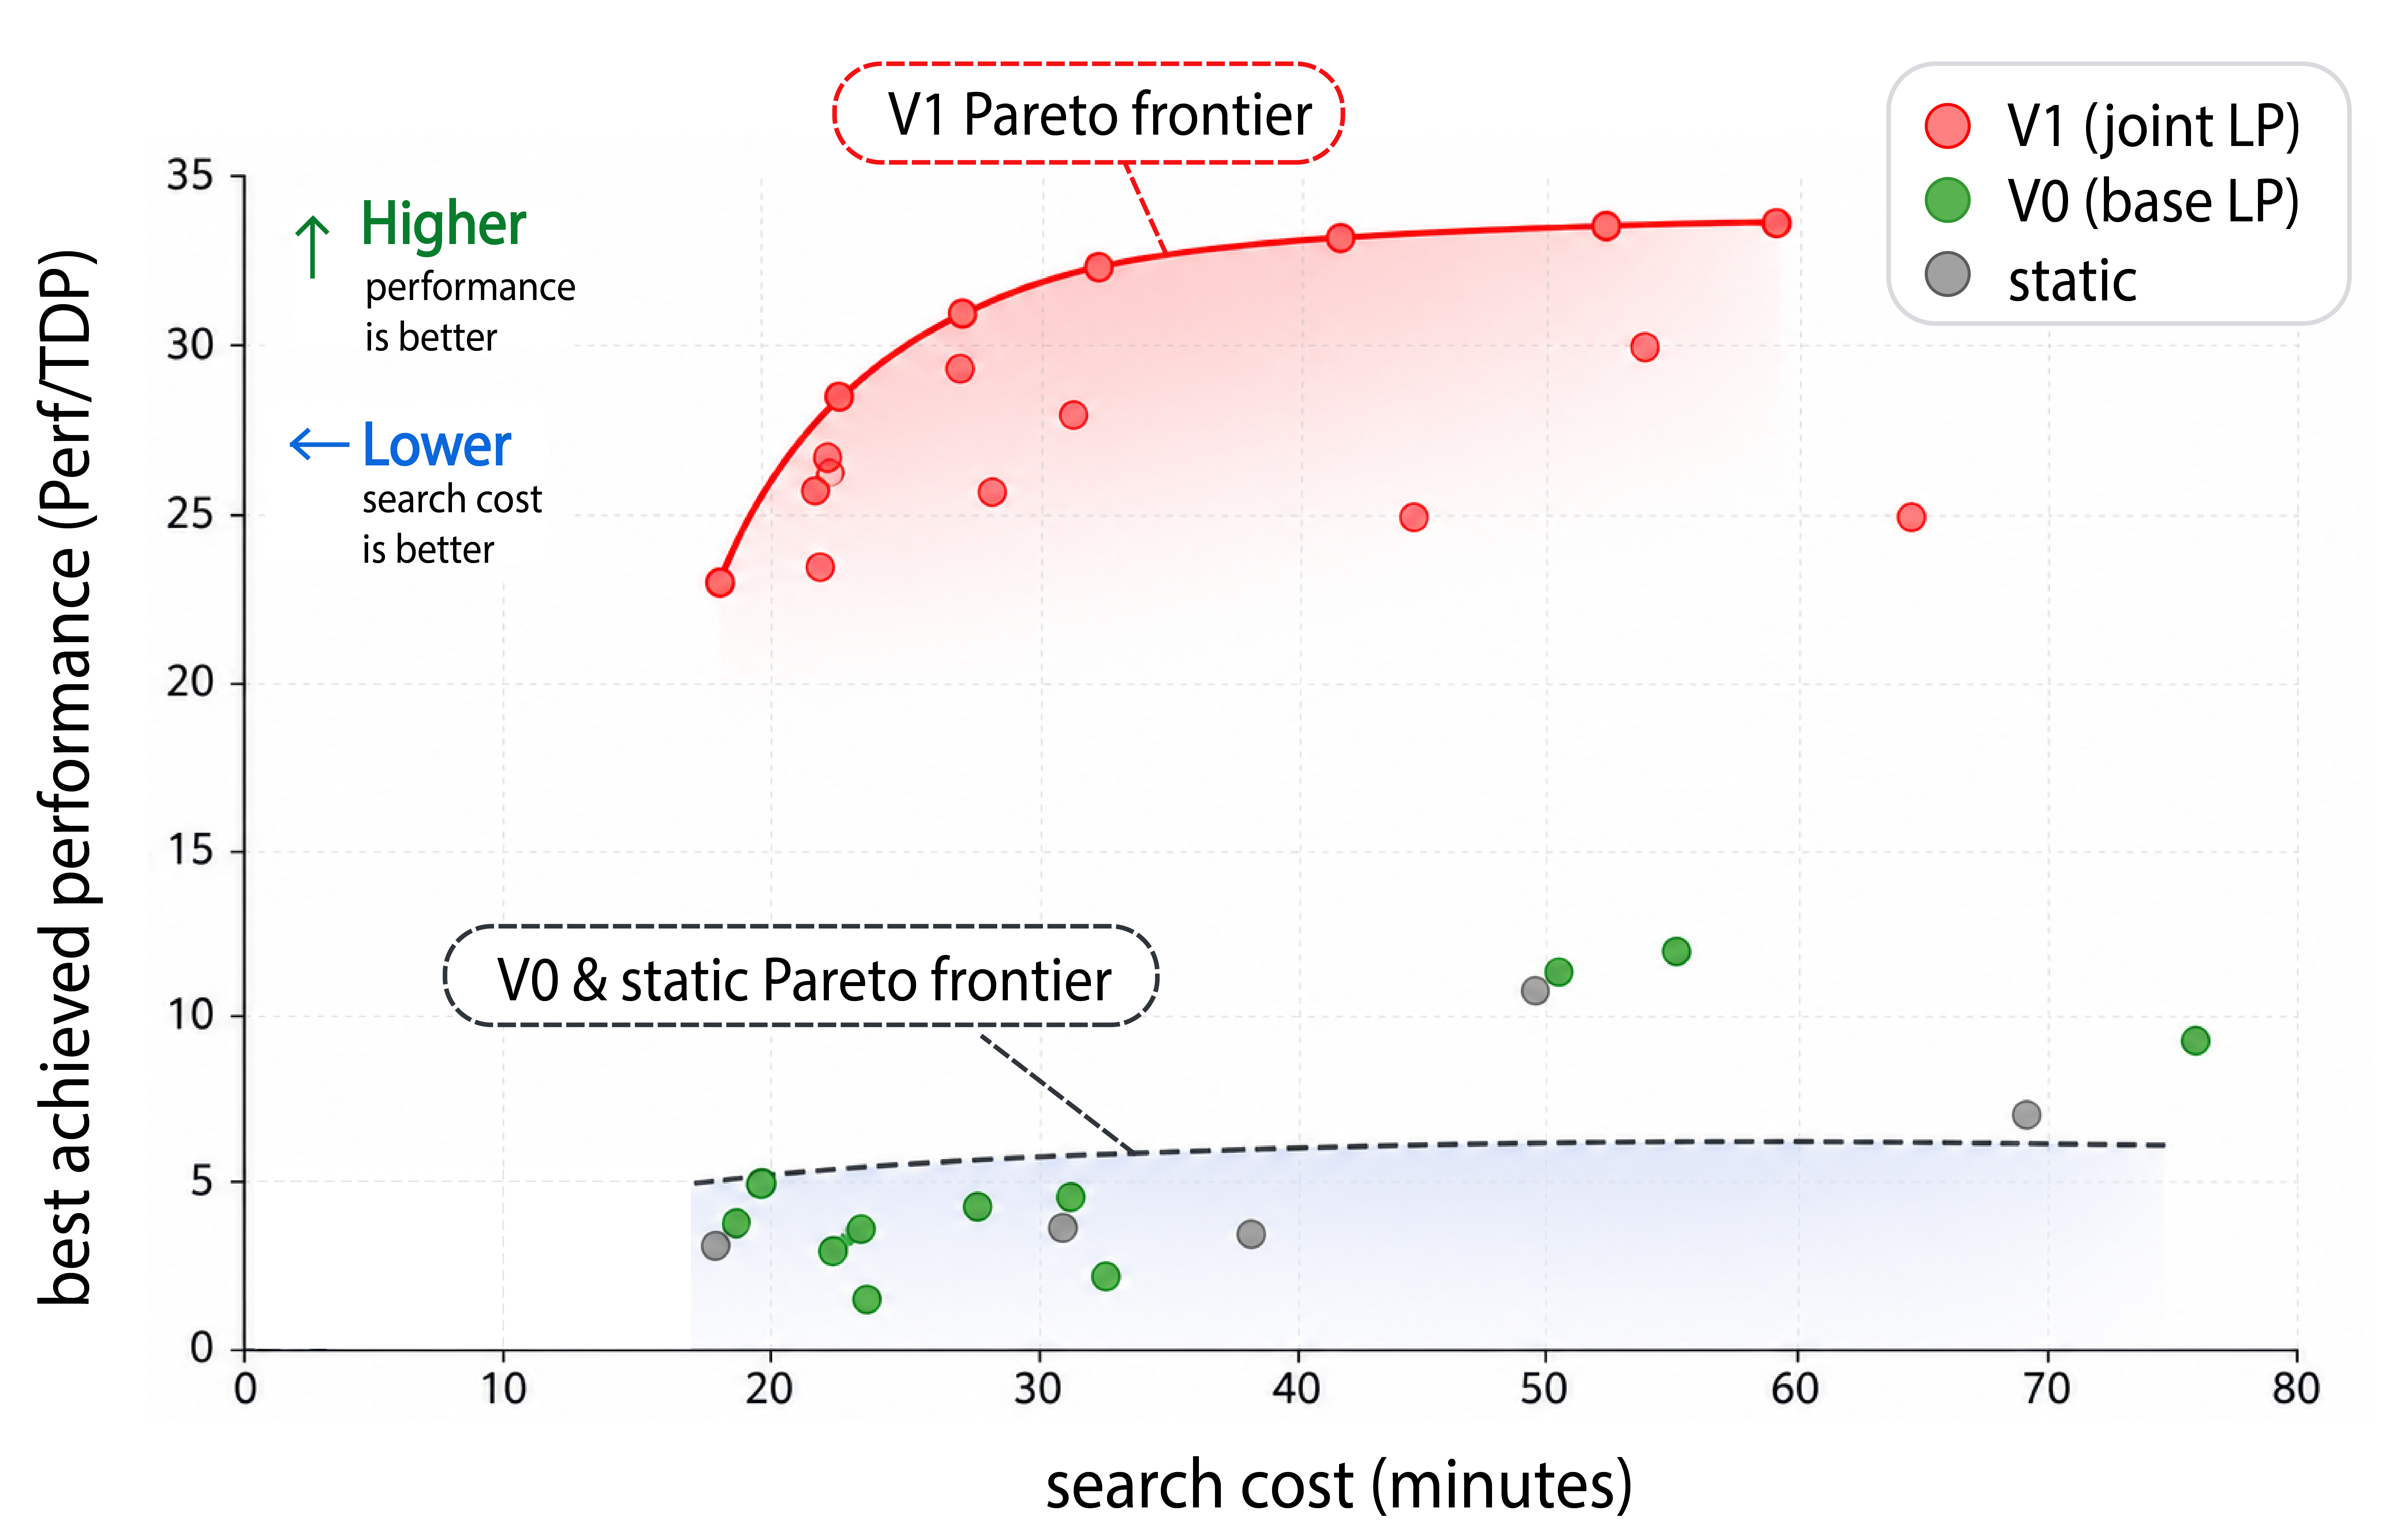
\includegraphics[width=0.7\linewidth]{figs/pareto_v2.png}
% %     \caption{pareto frontier plot}
% % \end{figure}
% \begin{figure}[ht!]
%     \centering
% 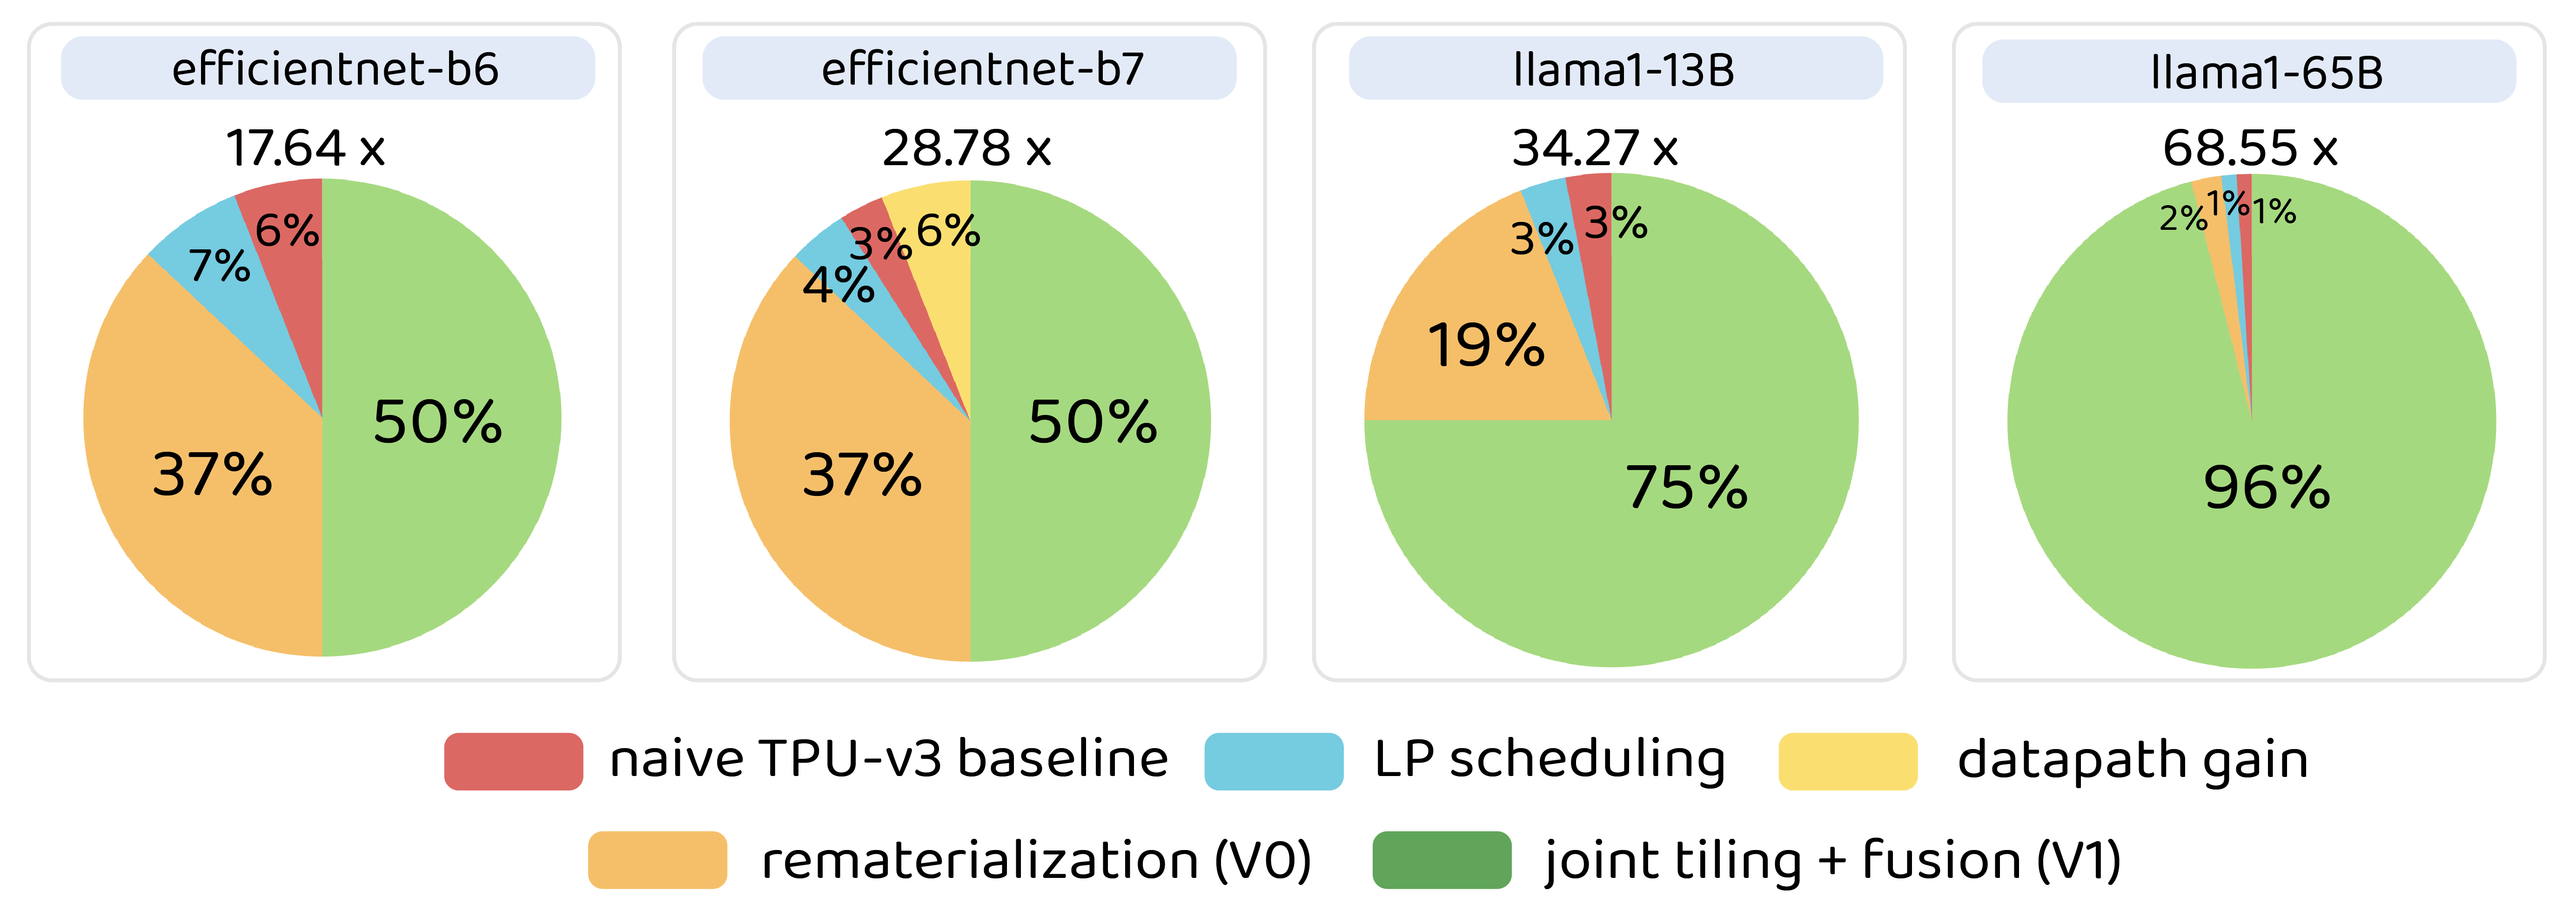
\includegraphics[width=0.85\linewidth]{fig3/speedup_decomposition_final_v2.png}
% \caption{Speedup decomposition over naive TPU-v3 baseline. Each pie shows the 
% relative contribution of four optimization sources to the total speedup. CHEETAH-V1 joint tiling + fusion dominates on all workloads, 
% especially on larger models where memory management is the primary bottleneck.}\label{fig:accel_decompose}
% \end{figure}
% \subsection{Static Baseline vs.\ CHEETAH-V0 vs.\ CHEETAH-V1 Unlock Progressive Gains}


% Figure~\ref{fig:accel_decompose} decomposes the total speedup over a naive TPU-v3 baseline into four sources: LP-based scheduling and fusion, datapath gain from hardware search, dynamic rematerialization (CHEETAH-V0), and joint tiling + fusion (CHEETAH-V1). Table~\ref{tab:LP_struct} gives side by side structural comparison of the V0 and V1 formulation matrices in greater detail. 

% The dominant contributor across all workloads is V1's joint tiling-fusion 
% optimization. On EfficientNet-B1, V1 accounts for 50\% of total speedup, 
% with LP scheduling (28\%) and datapath gain (22\%) splitting the remainder---and 
% no rematerialization benefit, consistent with B1's small activation footprint 
% fitting comfortably in Global Memory. B3--B4 show a similar 50\% V1 share, but 
% V0 rematerialization now contributes 25\%, reflecting the growing value of 
% recomputing large depthwise activations rather than reloading them from DRAM. 
% From B5 onward, V1's share rises sharply to 75--88\%, as the increasing 
% model size makes joint tiling-fusion the primary lever: memory management 
% dominates, and the remaining sources (LP scheduling, V0, datapath) each shrink 
% to single-digit percentages. The same pattern holds on Llama, where V1 accounts 
% for 83--87\% of the total speedup.

% Critically, Figure~\ref{fig:speedup} shows static fusion method is \emph{infeasible} on modern large models (Llama-70B, and DeepSeek-V3), because their large activation tensors cannot fit under a static pinning policy. The V0 formulation resolves feasibility on large models via dynamic placement, while V1 further improves by jointly selecting memory-efficient tiling configurations alongside placement, achieving feasibility across the entire workload suite. This demonstrates that joint optimization is not merely an incremental improvement but a qualitative capability unlock for large-scale models. Additional optimization details and observations are provided in Appendix~\ref{app:details}. We further provide two interesting examples of optimal tiling solutions the V1 formulation proposed in Appendix~\ref{app:tiling}.

% \begin{figure}[ht!] 
%     \centering
% 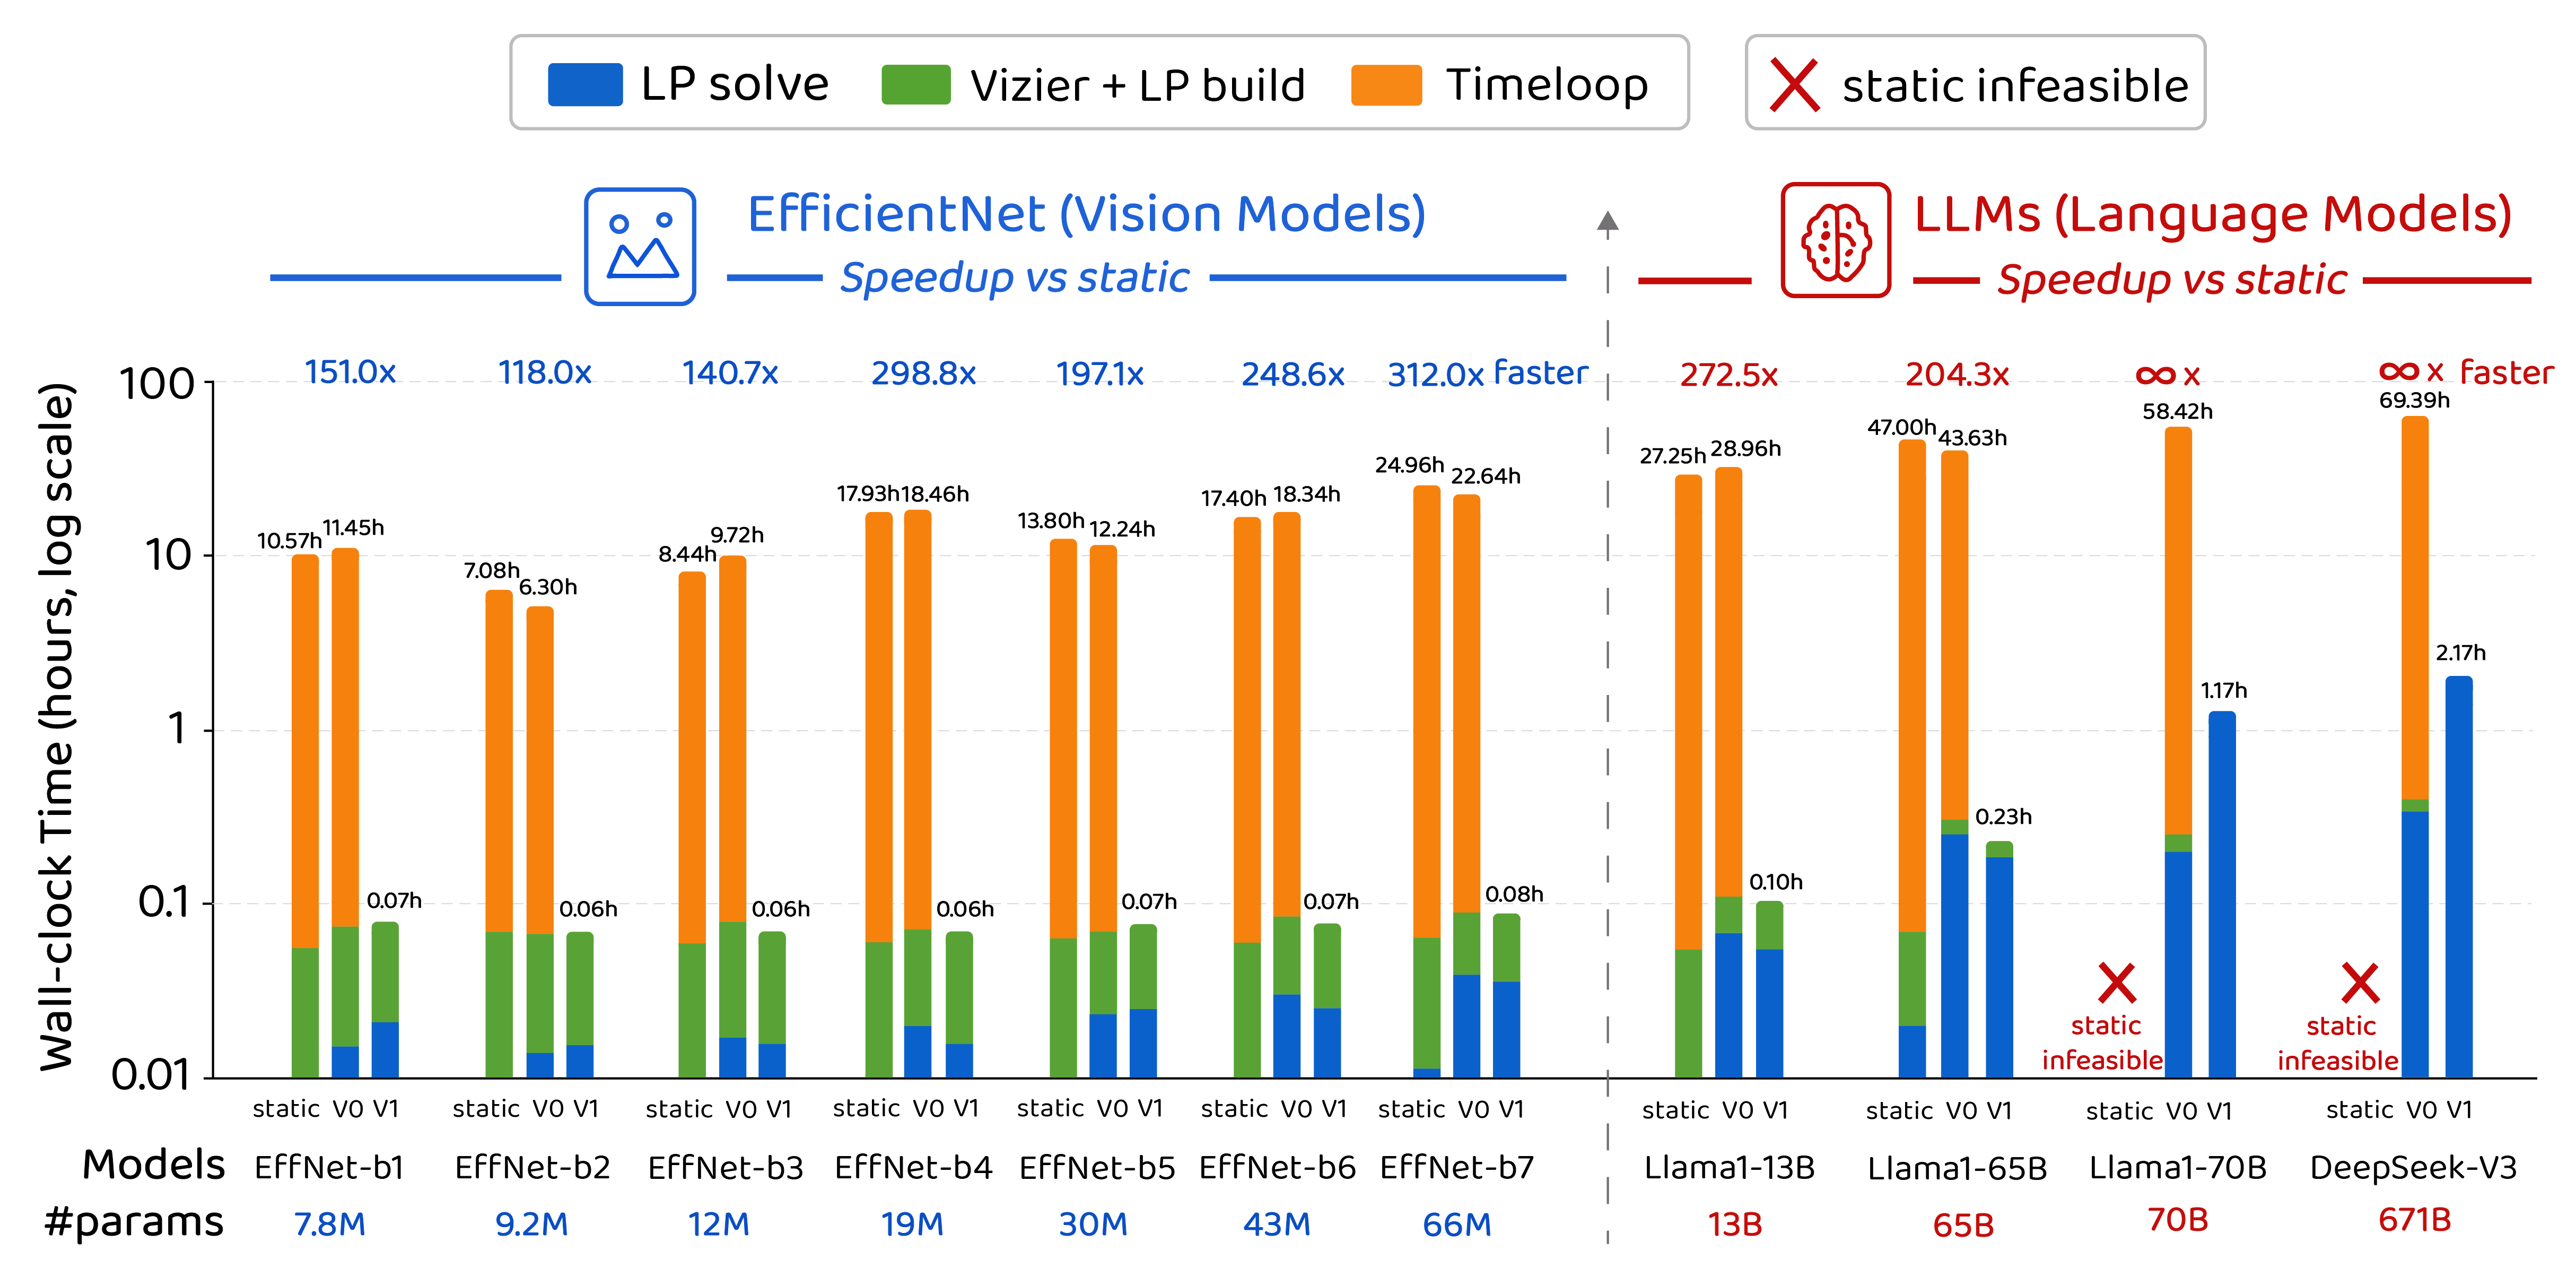
\includegraphics[width=1.0\linewidth]{fig3/wallclock_new_v5.png}
% \caption{Wall-clock time decomposition and performance acceleration across formulations: CHEETAH-V1's internalized tiling eliminates the Timeloop bottleneck, achieving up to 100--300$\times$ faster search than classical static method. Upper bars show wall-clock hours (log scale); annotations show speedup vs.\ static.}
% \label{fig:wallclock}
% \end{figure}

% \subsection{Wall-Clock Acceleration}

% Figure~\ref{fig:wallclock} reveals a striking practical advantage of V1: by internalizing tiling into the LP, it removes Timeloop from the per-trial critical path, collapsing each trial to a single Vizier-proposal and LP-solve step. On EfficientNet models, V1 completes 50 trials 151--312$\times$ faster than the static pipeline. On LLMs the acceleration is even more dramatic: V0 requires 58.42 hours on Llama-70B and 69.39 hours on DeepSeek-V3 for 50 trials, whereas V1 requires only 1.17 hours and 2.17 hours respectively---a ${\sim}93\%$ average reduction. This speedup arises because Timeloop accounts for over 99\% of per-trial latency in the sequential pipeline (Figure~\ref{fig:timeloop-time}), and V1 eliminates this bottleneck entirely via precomputed Pareto tiling sets that are reused across all Vizier trials sharing the same compute configuration class. The combination of higher speedup \emph{and} dramatically lower search cost makes V1 strictly dominant: it explores a larger feasible design space in a fraction of the wall-clock time.

% % This demonstrates that by exploiting structural invariance and GPU-accelerated mathematical optimization, CHEETAH-V1 reduces the end-to-end co-design search time from days to under 2.2 hours—a ${\sim}93\%$ average reduction—while discovering architectural points that deliver up to $35\times$ speedup over the TPU-v3 baseline.

% % Figure~\ref{fig:pareto} shows the Pareto frontier of best-achieved Perf/TDP versus wall-clock search cost. V1 strictly dominates both V0 and static at every time budget: within 10 minutes of search, V1 already exceeds the best Perf/TDP that V0 or static achieve after 60+ minutes. The V1 Pareto frontier reaches ${\sim}35\times$ Perf/TDP, roughly $3\times$ higher than the V0/static frontier at ${\sim}10\text{--}12\times$. This gap reflects two compounding advantages: V1 explores a strictly larger feasible region (joint tiling-fusion), and it eliminates Timeloop from the per-trial critical path, allowing more trials within any fixed time budget.



% \paragraph{LLM Architect vs.\ Optimizer.} Modelled on SkyDiscovery~\citep{skydiscover2026}, the LLM Architect prunes
% the outer search loop by proposing campaign patches rather than
% predicting raw performance. It analyses a Causal Ledger containing
% invalid rates, MFU, and solver diagnostics to suggest constrained
% hardware neighbourhoods for Vizier to explore locally. The V1 LP
% remains the ground-truth evaluator, supported by a Roofline Auditor
% that rejects physically impossible results.
% In a widened search space, the LLM loop reduces invalid evaluations
% from $24.5\%$ to $5.9\%$ on average --- a $4.1\times$ reduction in wasted
% trials --- while reaching the same optimal Perf/TDP scores as full-space
% Vizier. This demonstrates that the LLM's role is steering Bayesian
% optimisation toward feasible, workload-appropriate subspaces rather than
% replacing the solver. We provide exact prompts in Appendix~\ref{app:prompt} for full replication of results, as well as two specific cases studies of real-world use cases.

% % \subsubsection{LLM Architect vs. Optimizer}
% % The LLM Architect framework is modeled on SkyDiscover, and efficiently prunes the large outer hardware search loop by proposing campaign patches. Rather than predicting performance, the Architect reads a compact Causal Ledger containing invalid-rate history, MFU, roofline lower-bound checks, and LP diagnostics, then proposes a constrained hardware neighborhood for Vizier to search locally. The V1 LP remains the sole performance evaluator: for each candidate, it solves the joint tiling, fusion, placement, and rematerialization LP, while a deterministic Roofline Auditor rejects physically impossible results. In the widened V1 search space, all methods reach the same capped V1 Perf/TDP ceiling, so the key differentiator is search efficiency. The LLM loop reduces invalid hardware evaluations from 24.5\% under full-space Vizier to 5.9\% on average across five workloads, a 4.1× reduction in wasted trials, while preserving the same best V1 score. This shows that the LLM’s contribution is not replacing Vizier or the solver, but steering Bayesian optimization toward feasible, workload-appropriate architectural neighborhoods with far less wasted trials. This also sets the foundation for future work, where the LLM in the loop can adhere to follow more complex human reasoning signals.
% \begin{figure}[ht!]
%     \centering
% 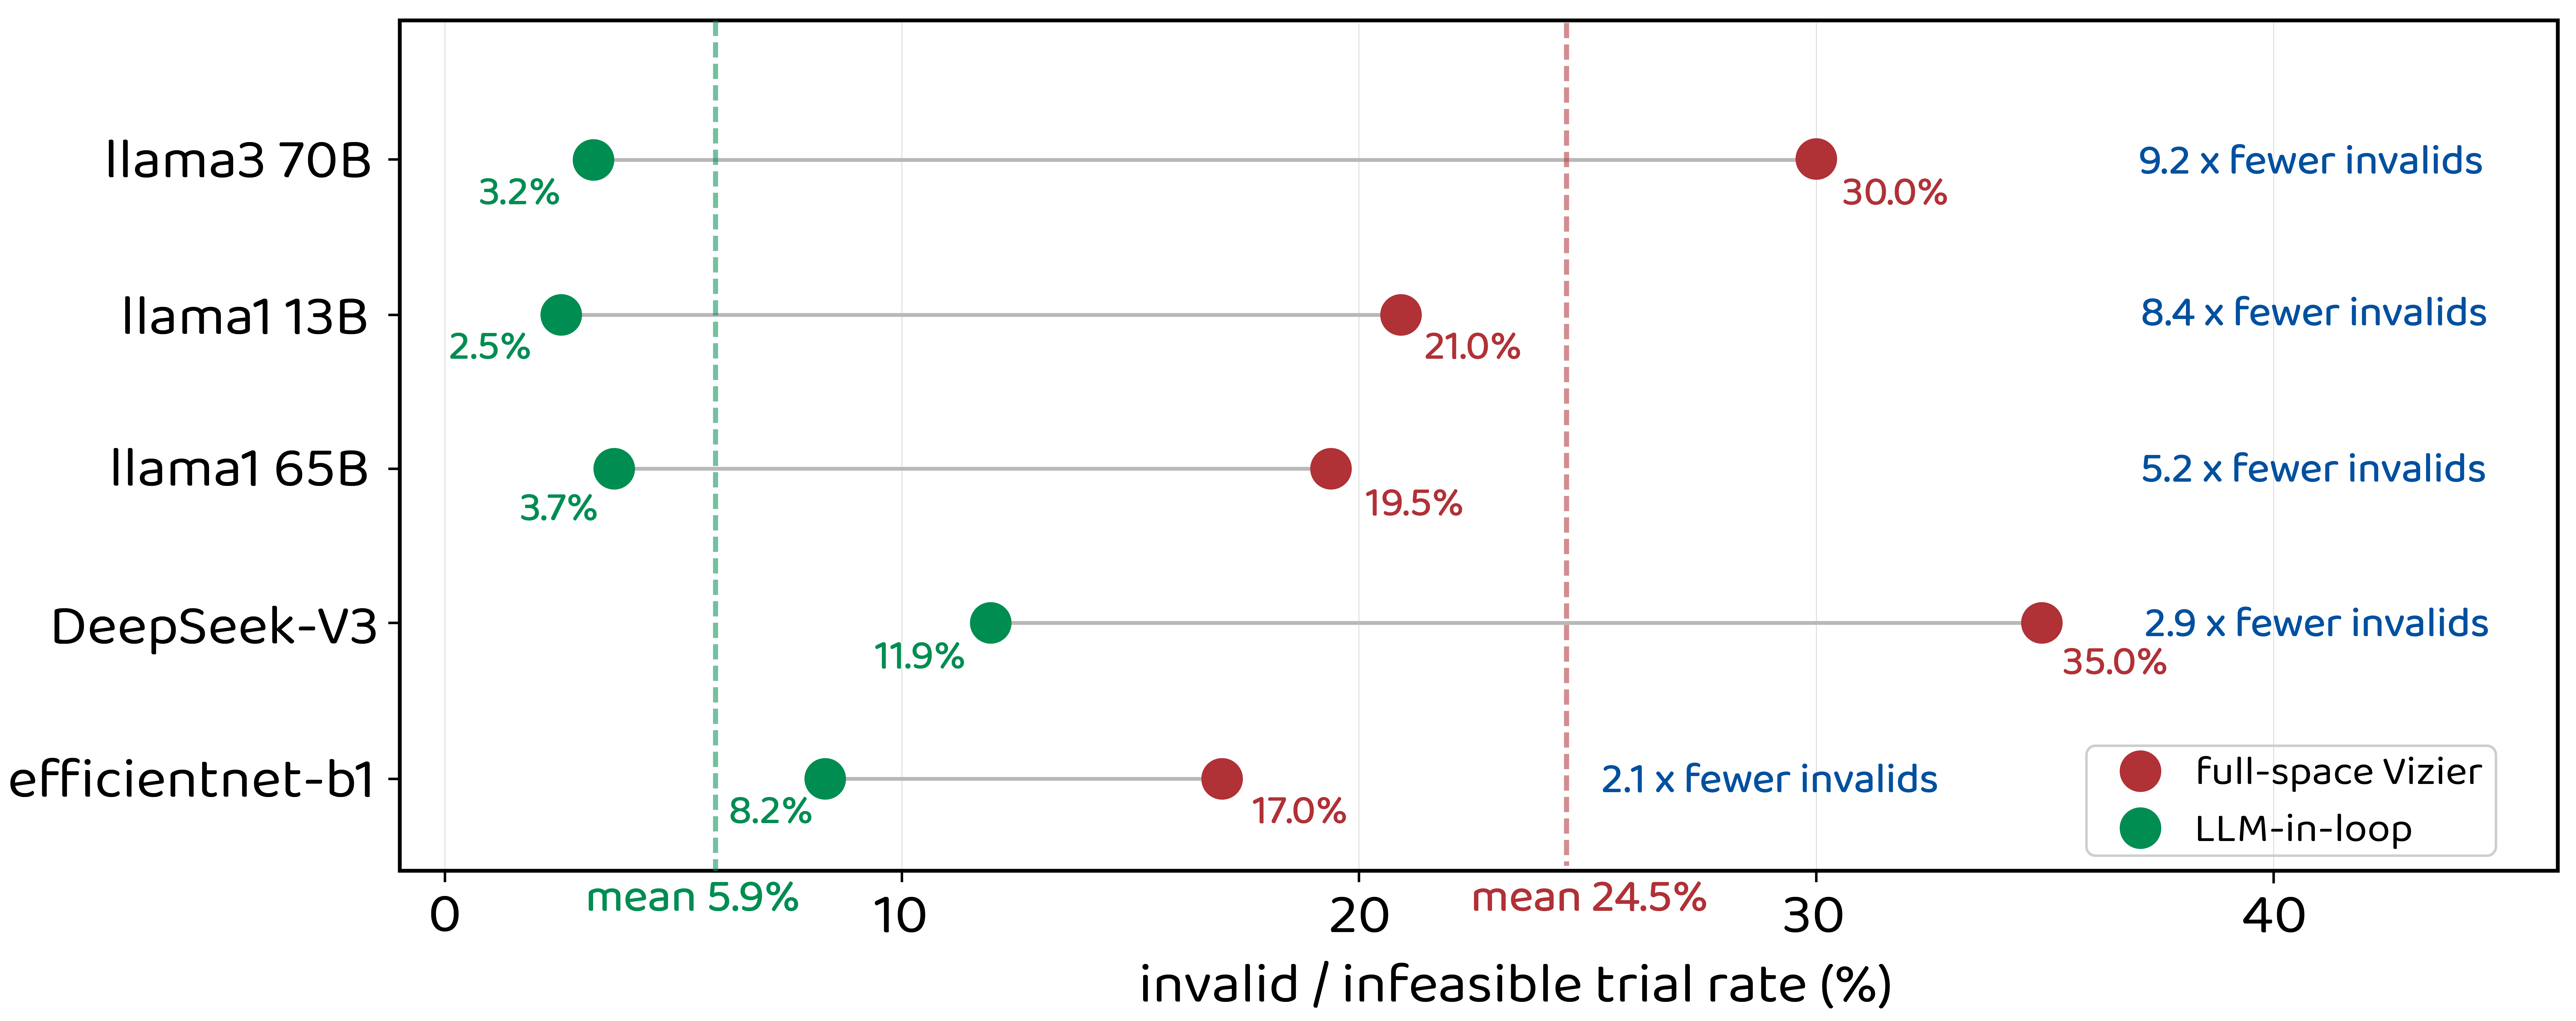
\includegraphics[width=0.85\linewidth]{fig3/llm_guide_v1.png}
% \caption{Invalid/infeasible trial rate (\%) for full-space Vizier vs.\ LLM-in-loop across five workloads. The LLM Architect reduces the mean invalid rate from 24.5\% to 5.9\% (4.1×$\times$
% × reduction), with the largest gains on LLM workloads where the hardware search space is most prone to infeasible configurations.}\label{fig:llm}
% \end{figure}



% % The LLM should not just ask, “What chip has the best Perf/TDP?” We aim to answer the question “Given this user’s workload and deployment goal, what is the architectural region to search for this deployment task?”. Therefore we have the LLM emit profile-conditioned campaigns that take specific user inference tasks into consideration. For each $(\text{deployment profile},\ \text{workload})$ cell, we ran a
% % 200-trial LLM-Architect experiment using the same Qwen2.5-7B-Instruct + LoRA with differing user input profiles. At the start of each round, the prompt was assembled from a fixed system
% % prompt, the active deployment profile, three few-shot examples, and a per-round user message containing the workload, recent feedback signals, current search bounds, and the causal ledger.
% % The Strategist returned a one-line JSON campaign patch, which the
% % validator accepted only if it was a strict legal subset of the parent space, satisfied hard rules such as patch-volume $\leq 10\%$, ridgepoint and MAC/BW constraints, and avoided forbidden regions.

% % Thus, the experiment isolates whether the profile-conditioned LLM prompt alone can steer the same V1 evaluator toward different hardware families under different deployment intents.



% % \todo{Compare convergence rate of LLM-guided hardware search vs.\ Vizier-only (Bayesian, LCS, random baselines) in the style of FAST Figure~11. Report:
% % \begin{itemize}
% %     \item Number of trials to reach $X\%$ of best Perf/TDP found by 5,000-trial Vizier
% %     \item Quality of LLM-proposed configurations vs.\ Vizier-proposed configurations
% %     \item Qualitative analysis of LLM reasoning about hardware bottlenecks
% % \end{itemize}
% % }

% % \subsubsection{ROI Analysis}

% % \todo{Update FAST's ROI analysis (Table~4) with the improved Perf/TDP numbers from FAST-CORGI. Report deployment volumes required to reach 1$\times$, 2$\times$, 4$\times$ ROI targets. If Perf/TDP improvements are larger than FAST's, the break-even deployment volume should decrease correspondingly.}

% % \subsubsection{Pareto Frontier}

% % \todo{Plot the Perf/TDP vs.\ area Pareto frontier for V1-optimized designs compared to FAST and TPU-v3 baseline, analogous to FAST Figure~12.}


% page limit edit

% % \section{Experiments}
% % \label{sec:experiments}
% % In all cases we use an adapted JAX PDLP solver for large models at LLama70-B and DeepSeekv3 scale across all three methods (Static, CHEETAH-V0, CHEETAH-V1); and use HiGHS as the default solver for all other smaller neural network models. In order to be consistent with prior work, our experimental results are presented as orders of speedup / performance against a vanilla TPU-V3. This is also since TPUs are targeted for NN accelerators (as opposed to GPUs), and the TPU-V3 has the most information publically released, making it possible for us to simluate it more accurately. 

% % \subsection{Experimental Setup}

% % \paragraph{Static Sequential Baseline.}
% % We compare against the static optimization FAST framework using a simulated TPU-v3 baseline normalized to a sub-10nm process technology, following the same methodology as Zhang \etal. The baseline simulator is well-correlated with production hardware: on average within 8.2\,$\pm$\,2.7\% of profiled TPU-v3 performance. We evaluate against a \emph{simulated} TPU-v3 baseline to account for optimistic simulator assumptions.

% % We evaluate across 11 representative workloads: EfficientNet-B1 through EfficientNet-B7, Llama13, 65, 70 models, and DeepSeek-V3-MoE. These workloads stress different parts of the hardware design space: EfficientNet stresses low-operational-intensity depthwise convolutions, while Llama and DeepSeek stress memory capacity, bandwidth, and large matrix operations. 

% % \textbf{Single-workload specialization.} Each neural network workload is optimized independently. This experiment measures the best workload-specific hardware found under a fixed trial budget and identifies architectural preferences such as Global Memory size, bandwidth, MAC count, and systolic shape. In the case of Staitic and V0 methods, the pipeline involves: Vizier - Timeloop - LP solver. In the case of the V1 method, the pipeline is simplified to Vizier - LP solver. In each case we iterate for 100 trials per method x NN. 

% % % \textbf{Fixed-hardware-workload generalization.} We search for general-purpose datapaths that perform well across the workload suite. The objective is a harmonic or geometric aggregation of per-workload Perf/TDP, forcing the search to balance CNN-style memory pressure and LLM-style compute/memory trade-offs.

% % \textbf{LLM-Architect guides outer search.} We the LLM-guided outer-loop controller which proposes search-space interventions for Vizier. The advantage of the CHEETAH-V1 formulation is it removes dependence of Timeloop in the loop. Therefore the loop is reduced to just Vizier-LP solve, which dramatically speeds up the iterative process, thus permitting the LLM-Architect outer loop. The LLM is only permitted to change the search neighborhood of Vizier's input, the strict LP formulation on the inner loop does not change. This ensures mathematical and physical constraints are upheld in the space of co-design. 

% % % \paragraph{Optimization framework.}
% % % For the outer hardware search loop, we use Google Vizier with LCS optimization and safe search, running 100 trials per experiment (method X NN x Exp). Each trial invokes the LP solver for the inner optimization. The Static and V0 methods additionally have Timeloop in the loop (Vizier-Timeloop-LP solve). The advantage of the v1 formulation is it removes dependance of Timeloop in the loop. Therefore the loop is reduced to just Vizier-Lp solve, which dramatically speeds up the iterative process, thus permitted the Strategic LLM outer loop.

% % We validate our framework through a multi-level audit process to ensure physical and numerical rigor.
% % \textbf{Roofline Auditor.}
% % A deterministic Roofline Auditor enforces physical feasibility by
% % verifying that LP-predicted latencies never fall below the theoretical
% % bound
% % \begin{equation}
% %     \mathrm{LB} = \max\!\left(t_{\mathrm{compute}},\;
% %     t_{\mathrm{memory}}\right),
% %     \label{eq:roofline_lb_val}
% % \end{equation}
% % where $t_{\mathrm{compute}}$ and $t_{\mathrm{memory}}$ represent the
% % peak compute and memory bandwidth floors, respectively.
% % All reported V0/V1 results are roofline-feasible with valid
% % $\mathrm{MFU}_{\mathrm{bound}}$ and memory utilization metrics.

% % \textbf{Campaign Validator.}
% % A deterministic Campaign Validator legalizes LLM-proposed architectural
% % neighbourhoods by enforcing hard hardware constraints — including TDP
% % caps, area limits, and power-of-two parameter ranges — prior to Vizier
% % sampling.

% % \textbf{Causal Ledger.}
% % A Causal Ledger tracks LLM interventions and observed outcomes,
% % preventing redundant exploration of empirically invalid regions and
% % ensuring full auditability of the search loop.

% % \textbf{Solver Diagnostics.}
% % We monitor solver diagnostics including primal/dual residuals, duality
% % gap, and rounding gap. Designs are treated as trustworthy only when both
% % the continuous LP relaxation and the rounded integer solution are
% % numerically well-behaved.


% % \subsection{Main Results}

% % % \subsubsection{V0 vs.\ FAST Static Fusion}

% % % \todo{Insert results table and figure comparing V0 (time-indexed placement + rematerialization) against FAST's static fusion ILP on all benchmarks. Key metrics: Perf/TDP improvement, fusion efficiency (\% of DRAM stall time eliminated), rematerialization frequency (how often does the solver choose to recompute rather than reload?).}

% % % \paragraph{Expected findings.}
% % % V0's dynamic placement should show the largest gains on workloads with: (1)~tight Global Memory budgets where static pinning wastes capacity on tensors that are only needed briefly, (2)~long dependency chains where tensor lifetimes vary substantially, and (3)~cheap-to-recompute operations with large activations (\eg, depthwise convolutions in EfficientNet).

% % % \subsubsection{V1 vs.\ V0: Joint Tiling and Fusion}

% % % \todo{Insert results table and figure comparing V1 against V0 on all benchmarks. Key metrics: Perf/TDP improvement, number of operations where V1 selects a different tiling configuration than Timeloop's greedy choice, and the resulting compute efficiency vs.\ fusion trade-off.}

% % % \paragraph{Expected findings.}
% % % V1 should show the largest gains on architectures with highly diverse layer types where a single tiling configuration cannot serve all operations well. EfficientNet (depthwise + pointwise convolutions with 100$\times$ variation in working-set sizes) and hybrid CNN-transformer models (convolutions + attention + MLP with fundamentally different compute-memory profiles) are expected to benefit most.


% % % \subsubsection{stiatic vs v0 vs v1}
% % % \begin{figure}[ht!]
% % %     \centering
% % %     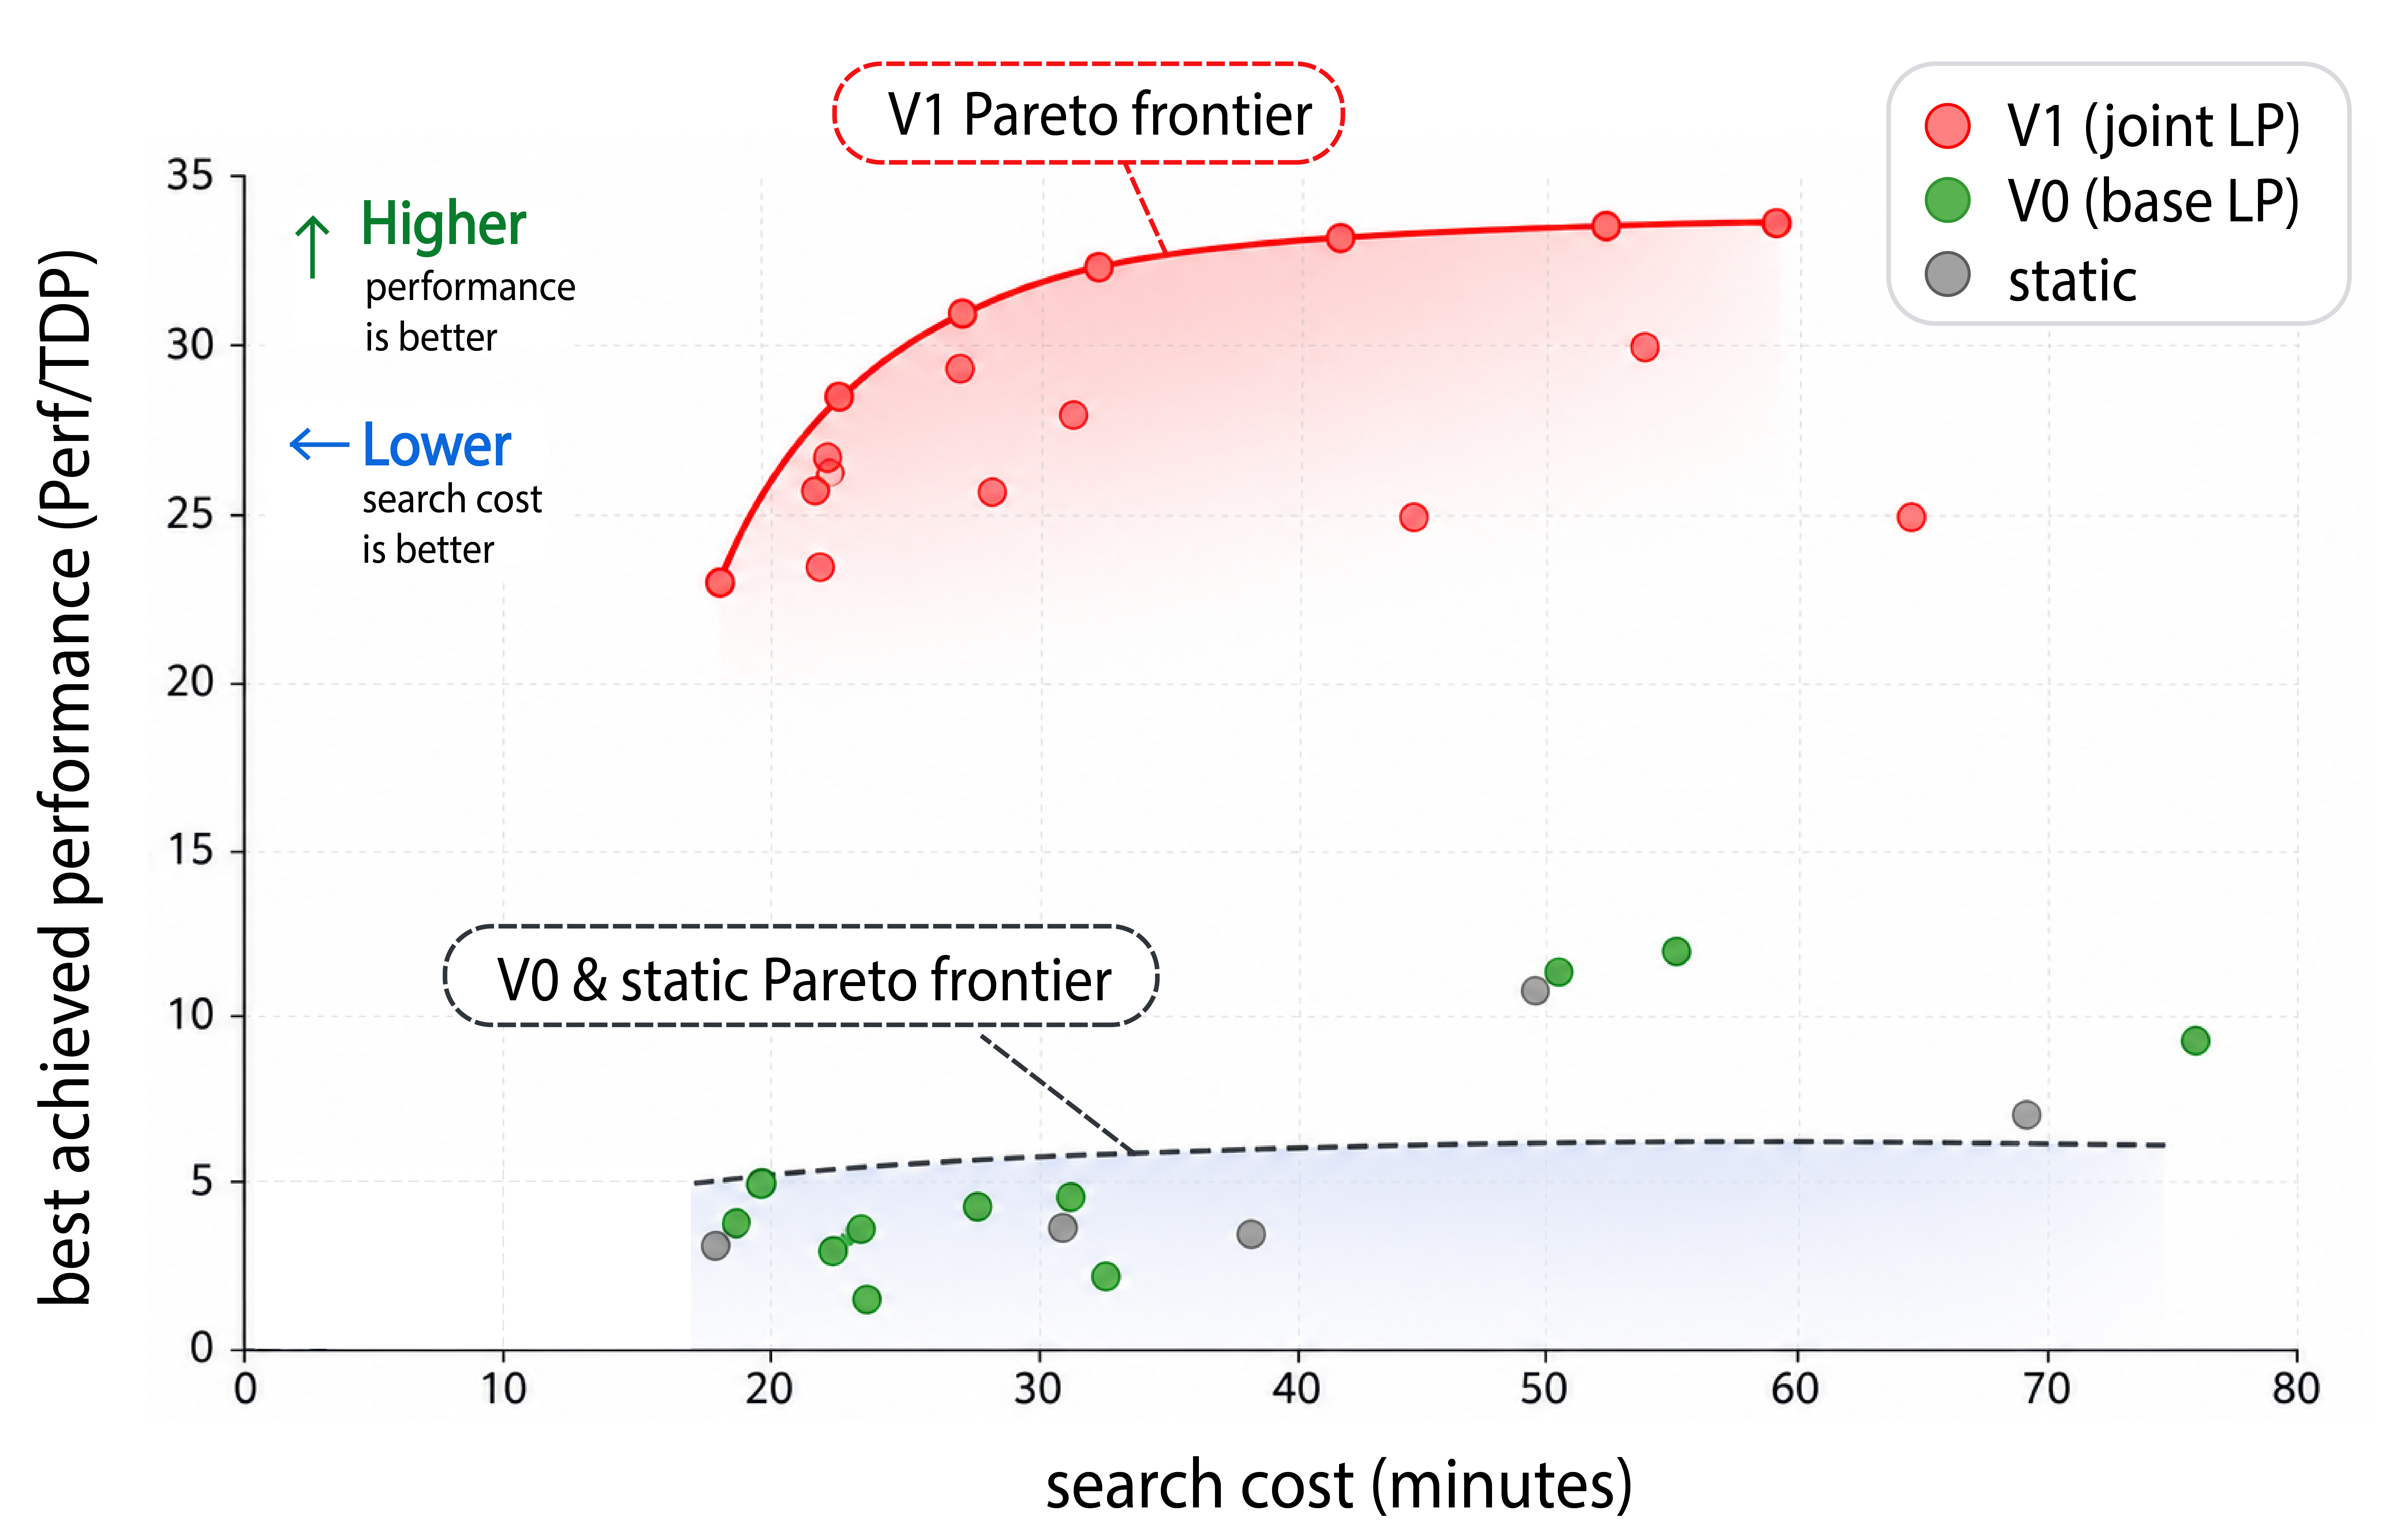
\includegraphics[width=0.7\linewidth]{figs/pareto_v2.png}
% % %     \caption{pareto frontier plot}
% % % \end{figure}
% % \begin{figure}[ht!]
% %     \centering
% % 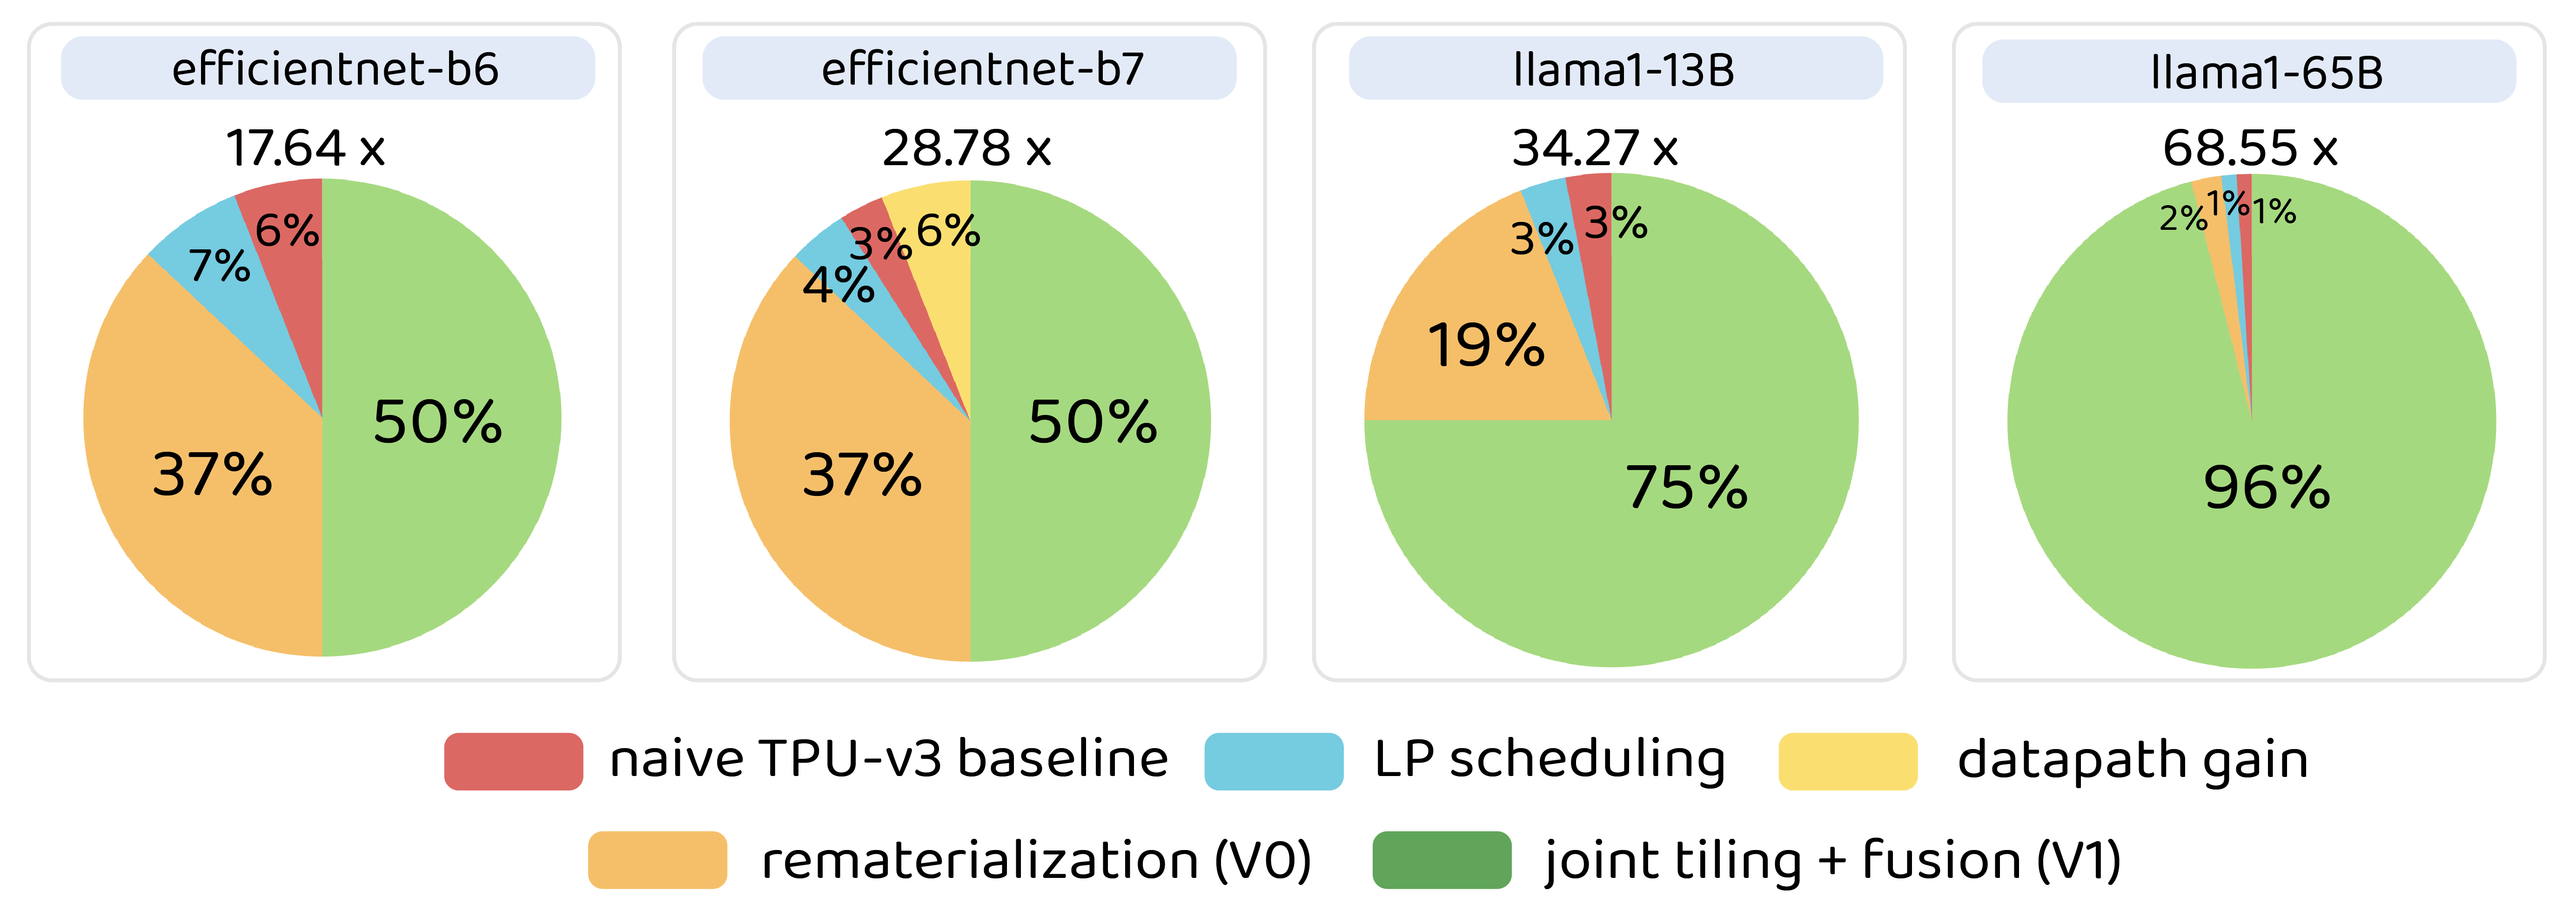
\includegraphics[width=0.85\linewidth]{fig3/speedup_decomposition_final_v2.png}
% % \caption{Speedup decomposition over naive TPU-v3 baseline. Each pie shows the 
% % relative contribution of four optimization sources to the total speedup. CHEETAH-V1 joint tiling + fusion dominates on all workloads, 
% % especially on larger models where memory management is the primary bottleneck.}\label{fig:accel_decompose}
% % \end{figure}
% % \subsubsection{Static Baseline vs.\ CHEETAH-V0 vs.\ CHEETAH-V1 Unlock Progressive Gains}


% % Figure~\ref{fig:accel_decompose} decomposes the total speedup over a naive TPU-v3 baseline into four sources: LP-based scheduling and fusion, datapath gain from hardware search, dynamic rematerialization (CHEETAH-V0), and joint tiling + fusion (CHEETAH-V1).

% % The dominant contributor across all workloads is V1's joint tiling-fusion 
% % optimization. On EfficientNet-B1, V1 accounts for 50\% of total speedup, 
% % with LP scheduling (28\%) and datapath gain (22\%) splitting the remainder---and 
% % no rematerialization benefit, consistent with B1's small activation footprint 
% % fitting comfortably in Global Memory. B3--B4 show a similar 50\% V1 share, but 
% % V0 rematerialization now contributes 25\%, reflecting the growing value of 
% % recomputing large depthwise activations rather than reloading them from DRAM. 
% % From B5 onward, V1's share rises sharply to 75--88\%, as the increasing 
% % model size makes joint tiling-fusion the primary lever: memory management 
% % dominates, and the remaining sources (LP scheduling, V0, datapath) each shrink 
% % to single-digit percentages. The same pattern holds on Llama, where V1 accounts 
% % for 83--87\% of the total speedup.

% % % \begin{wrapfigure}{r}{0.48\textwidth}
% % %     \centering
% % %     \vspace{-12pt}
% % %     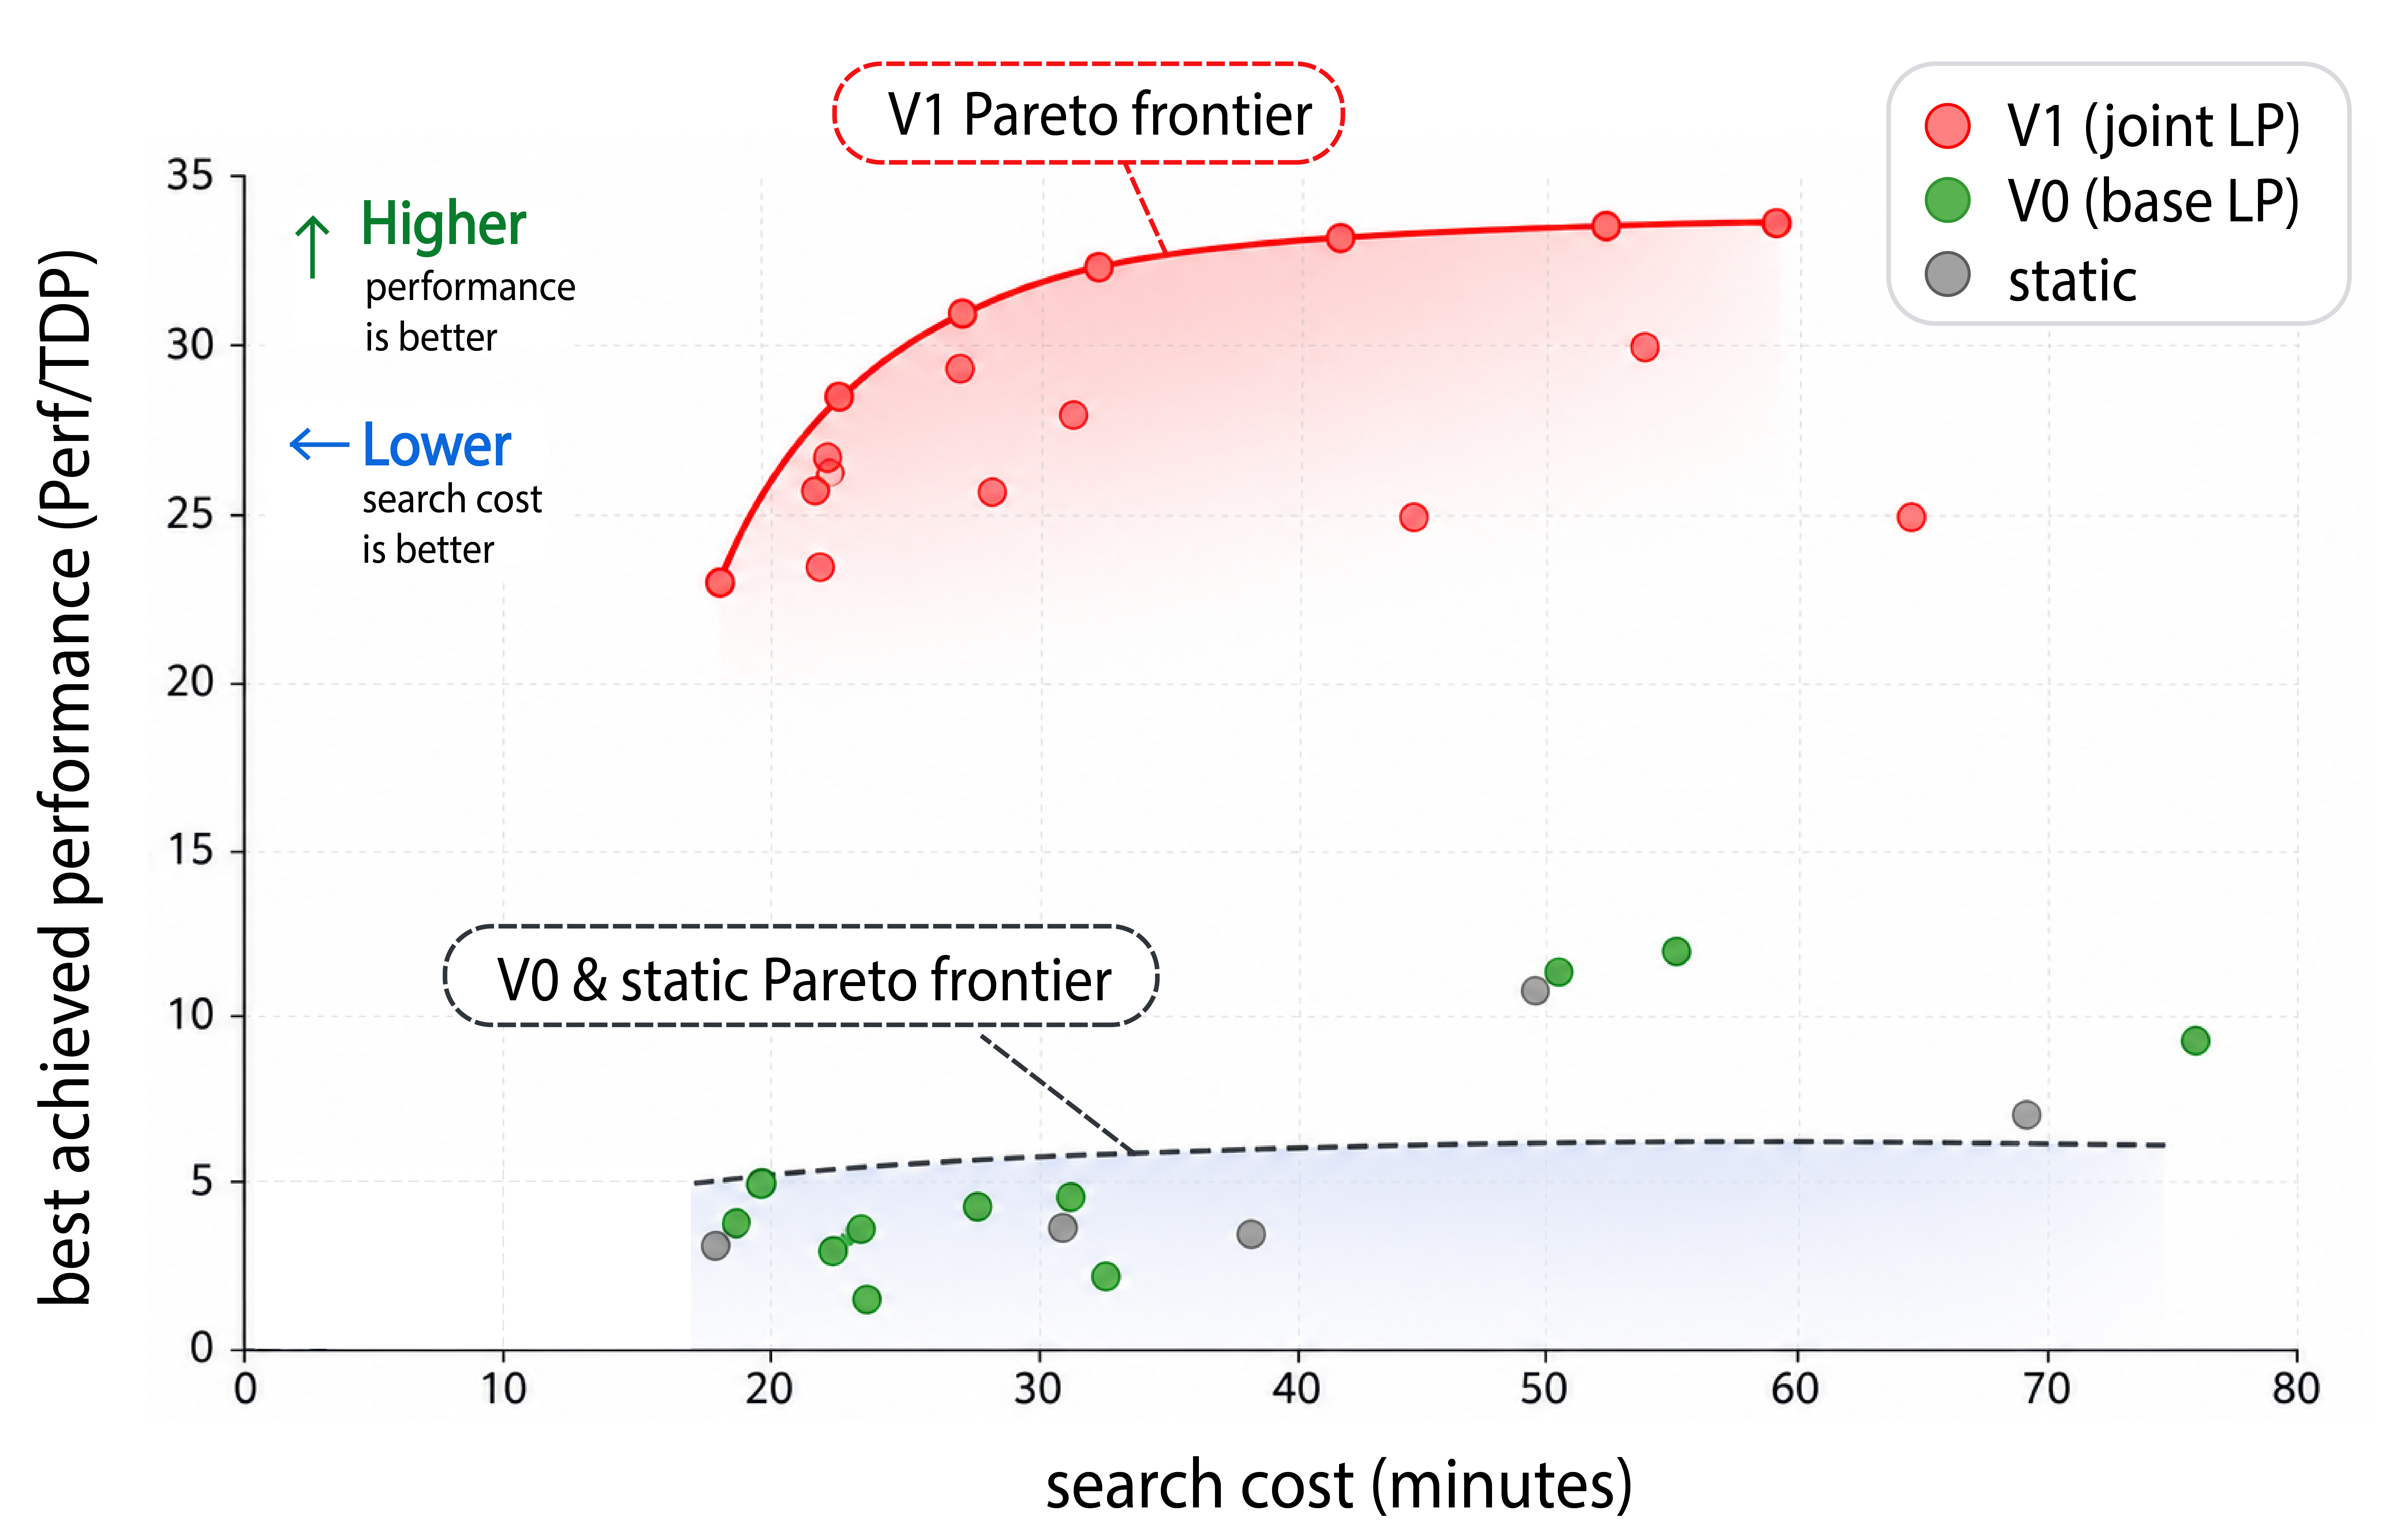
\includegraphics[width=0.48\textwidth]{figs/pareto_v2.png}
% % %     \vspace{-18pt}
% % %     \caption{Search cost vs.\ Perf/TDP Pareto frontier. V1 dominates V0 and static across all time budgets.}
% % %     \label{fig:pareto}
% % %     \vspace{-10pt}
% % % \end{wrapfigure}

% % Critically, Figure~\ref{fig:speedup} shows static fusion method is \emph{infeasible} on modern large models (Llama-70B, and DeepSeek-V3), because their large activation tensors cannot fit under a static pinning policy. The V0 formulation resolves feasibility for on large models via dynamic placement but remains time-intensive for a small number of 50 trials: measuring 58.42 hours on Llama-70B and 69.39 hours on DeepSeek-V3 (Figure~\ref{fig:wallclock}). In contrast Figures~\ref{fig:wallclock} and ~\ref{fig:speedup}, show the CHEETAH-V1 formulation out performs comparitive strategies in terms of speedup against the TPU-V3 baseline, and require only 1.17 hours on Llama-70B and 2.17 hours on DeepSeekv3 for 50 trails---a ${\sim}93\%$ average reduction. The powerful joint formulation is able to select memory-efficient tiling configurations alongside placement, achieving feasibility across the entire workload suite, demonstrating that joint optimization is not merely an incremental improvement but a qualitative capability unlock for large-scale models.

% % % This demonstrates that by exploiting structural invariance and GPU-accelerated mathematical optimization, CHEETAH-V1 reduces the end-to-end co-design search time from days to under 2.2 hours—a ${\sim}93\%$ average reduction—while discovering architectural points that deliver up to $35\times$ speedup over the TPU-v3 baseline.

% % % Figure~\ref{fig:pareto} shows the Pareto frontier of best-achieved Perf/TDP versus wall-clock search cost. V1 strictly dominates both V0 and static at every time budget: within 10 minutes of search, V1 already exceeds the best Perf/TDP that V0 or static achieve after 60+ minutes. The V1 Pareto frontier reaches ${\sim}35\times$ Perf/TDP, roughly $3\times$ higher than the V0/static frontier at ${\sim}10\text{--}12\times$. This gap reflects two compounding advantages: V1 explores a strictly larger feasible region (joint tiling-fusion), and it eliminates Timeloop from the per-trial critical path, allowing more trials within any fixed time budget.



% % \paragraph{Practical insight.}
% % Both LPs are extreme-aspect-ratio sparse: for \texttt{llama3\_70b},
% % $m, n \sim 10^6$ and $\mathrm{nnz} \sim 5 \times 10^6$, giving roughly
% % 1 nonzero per million matrix entries.
% % The time-band structure means a coordinate-descent or stochastic PDHG
% % solver would converge in $\mathcal{O}(T)$ sweeps if bands were the only
% % structure.
% % The capacity rows in both V0 and V1 LP formulations are the sole feature breaking strict banded structure, and they are precisely what couples the schedule globally. This is the desired behavior of a memory-aware placement formulation.

% % % \todo{Report LP solve times for V0 and V1 across all benchmarks. Compare wall-clock time per trial against FAST's SCIP-based ILP solver (20 min timeout). Report LP relaxation gap: how often do fractional solutions need integer rounding, and what is the quality loss from rounding?}

% % \paragraph{Structural invariance.}
% % For a fixed workload and LP formulation, the LP constraint matrix
% % has an invariant sparsity pattern across trials: the row/column
% % dimensions and nonzero locations are determined only by the model graph structure — layer count $L$, timestep count $T$, edge set $E$, and Pareto count $C$ — not by the hardware candidate.
% % Vizier changes only numerical values such as cycle coefficients,
% % memory-capacity bounds, bandwidth-scaled access costs, objective weights, and TDP/area parameters. 
% % This invariance allows us to reuse the same sparse matrix structure,
% % variable ordering, block layout, and JIT-compiled sparse kernels in our adapted JAX PDLP solver across all hardware trials for a given workload.

% % Numerically, we apply the same diagonal preconditioning pipeline
% % on each trial: a structural presolve with 20 log-geomean Ruiz iterations, followed by the PDLP preprocessing stack with 10 infinity-norm Ruiz iterations and one Pock--Chambolle $\ell_1$-scaling pass. This two-stage diagonal scaling handles the mixed coefficient magnitudes present in V0/V1 matrices — large byte-valued capacity rows together with $\pm 1$ persistence rows — without requiring a fragile matrix factorization.

% % In production, this preconditioning pipeline is reused structurally across trials, recomputes only cheap diagonal scalings, finishes in under one second for matrices with approximately $5 \times 10^6$ nonzeros, and avoids factorization failures entirely because it consists only of $D_1 A D_2$ arithmetic.

% % \subsubsection{LLM Architect vs. Optimizer}
% % The LLM Architect framework is modeled on SkyDiscover, and efficiently prunes the large outer hardware search loop by proposing campaign patches. Rather than predicting performance, the Architect reads a compact Causal Ledger containing invalid-rate history, MFU, roofline lower-bound checks, and LP diagnostics, then proposes a constrained hardware neighborhood for Vizier to search locally. The V1 LP remains the sole performance evaluator: for each candidate, it solves the joint tiling, fusion, placement, and rematerialization LP, while a deterministic Roofline Auditor rejects physically impossible results. In the widened V1 search space, all methods reach the same capped V1 Perf/TDP ceiling, so the key differentiator is search efficiency. The LLM loop reduces invalid hardware evaluations from 24.5\% under full-space Vizier to 5.9\% on average across five workloads, a 4.1× reduction in wasted trials, while preserving the same best V1 score. This shows that the LLM’s contribution is not replacing Vizier or the solver, but steering Bayesian optimization toward feasible, workload-appropriate architectural neighborhoods with far less wasted trials. This also sets the foundation for future work, where the LLM in the loop can adhere to follow more complex human reasoning signals.
% % \begin{figure}[ht!]
% %     \centering
% % 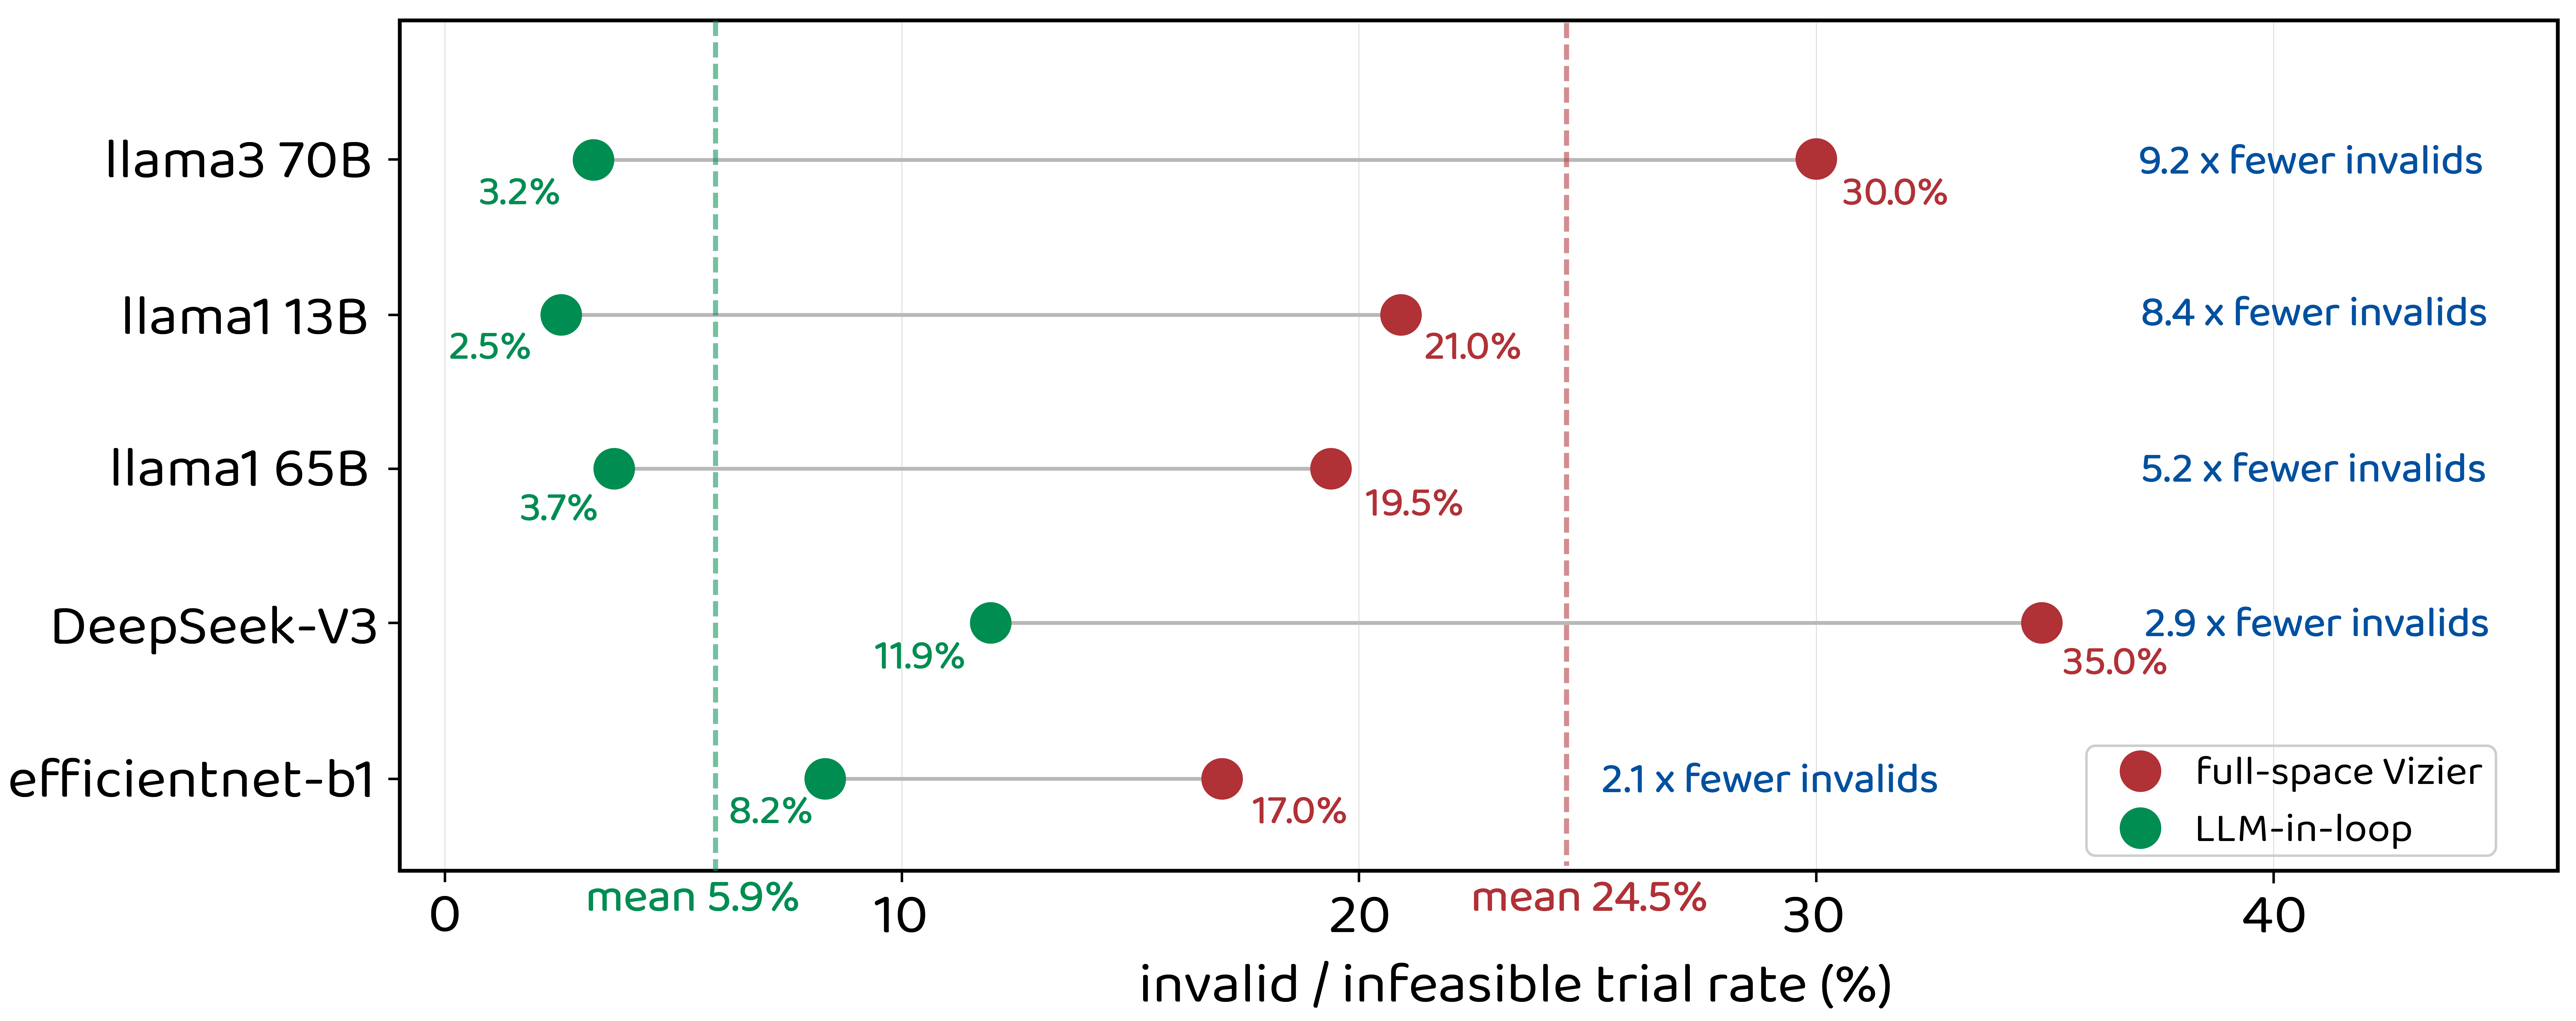
\includegraphics[width=0.85\linewidth]{fig3/llm_guide_v1.png}
% % \caption{Strategic Intelligence vs. Stochastic Brute Force}\label{fig:llm}
% % \end{figure}



% % % The LLM should not just ask, “What chip has the best Perf/TDP?” We aim to answer the question “Given this user’s workload and deployment goal, what is the architectural region to search for this deployment task?”. Therefore we have the LLM emit profile-conditioned campaigns that take specific user inference tasks into consideration. For each $(\text{deployment profile},\ \text{workload})$ cell, we ran a
% % % 200-trial LLM-Architect experiment using the same Qwen2.5-7B-Instruct + LoRA with differing user input profiles. At the start of each round, the prompt was assembled from a fixed system
% % % prompt, the active deployment profile, three few-shot examples, and a per-round user message containing the workload, recent feedback signals, current search bounds, and the causal ledger.
% % % The Strategist returned a one-line JSON campaign patch, which the
% % % validator accepted only if it was a strict legal subset of the parent space, satisfied hard rules such as patch-volume $\leq 10\%$, ridgepoint and MAC/BW constraints, and avoided forbidden regions.

% % % Thus, the experiment isolates whether the profile-conditioned LLM prompt alone can steer the same V1 evaluator toward different hardware families under different deployment intents.



% % % \todo{Compare convergence rate of LLM-guided hardware search vs.\ Vizier-only (Bayesian, LCS, random baselines) in the style of FAST Figure~11. Report:
% % % \begin{itemize}
% % %     \item Number of trials to reach $X\%$ of best Perf/TDP found by 5,000-trial Vizier
% % %     \item Quality of LLM-proposed configurations vs.\ Vizier-proposed configurations
% % %     \item Qualitative analysis of LLM reasoning about hardware bottlenecks
% % % \end{itemize}
% % % }

% % % \subsubsection{ROI Analysis}

% % % \todo{Update FAST's ROI analysis (Table~4) with the improved Perf/TDP numbers from FAST-CORGI. Report deployment volumes required to reach 1$\times$, 2$\times$, 4$\times$ ROI targets. If Perf/TDP improvements are larger than FAST's, the break-even deployment volume should decrease correspondingly.}

% % % \subsubsection{Pareto Frontier}

% % % \todo{Plot the Perf/TDP vs.\ area Pareto frontier for V1-optimized designs compared to FAST and TPU-v3 baseline, analogous to FAST Figure~12.}


% % edit for page limit

% \section{Experiments}
% \label{sec:experiments}
% We implement an adapted JAX PDLP solver for large-scale models (Llama-70B and DeepSeek-V3) across all formulations (Static, V0, V1), while employing HiGHS for smaller networks. To maintain consistency with prior research, results are reported as speedup relative to a simulated TPU-v3 baseline. The TPU-v3 is selected as a benchmark because its architecture is purpose-built for neural network acceleration and its publicly available specifications permit high-fidelity simulation.

% \subsection{Experimental Setup}

% \paragraph{Static Sequential Baseline.}
% We compare against the static optimization FAST framework using a simulated TPU-v3 baseline normalized to a sub-10nm process technology, following the same methodology as Zhang \etal. The baseline simulator is well-correlated with production hardware: on average within 8.2\,$\pm$\,2.7\% of profiled TPU-v3 performance. We evaluate against a \emph{simulated} TPU-v3 baseline to account for optimistic simulator assumptions. We evaluate across 11 representative workloads: EfficientNet-B1 through EfficientNet-B7, Llama13, 65, 70 models, and DeepSeek-V3-MoE. These workloads stress different parts of the hardware design space: EfficientNet stresses low-operational-intensity depthwise convolutions, while Llama and DeepSeek stress memory capacity, bandwidth, and large matrix operations. 

% \textbf{Single-workload specialization.} Each neural network workload is optimized independently. This experiment measures the best workload-specific hardware found under a fixed trial budget and identifies architectural preferences such as Global Memory size, bandwidth, MAC count, and systolic shape. In the case of Staitic and V0 methods, the pipeline involves: Vizier - Timeloop - LP solver. In the case of the V1 method, the pipeline is simplified to Vizier - LP solver. In each case we iterate for 100 trials per method x NN. 

% % \textbf{Fixed-hardware-workload generalization.} We search for general-purpose datapaths that perform well across the workload suite. The objective is a harmonic or geometric aggregation of per-workload Perf/TDP, forcing the search to balance CNN-style memory pressure and LLM-style compute/memory trade-offs.

% \textbf{LLM-Architect guides outer search.} We the LLM-guided outer-loop controller which proposes search-space interventions for Vizier. The advantage of the CHEETAH-V1 formulation is it removes dependence of Timeloop in the loop. Therefore the loop is reduced to just Vizier-LP solve, which dramatically speeds up the iterative process, thus permitting the LLM-Architect outer loop. The LLM is only permitted to change the search neighborhood of Vizier's input, the strict LP formulation on the inner loop does not change. This ensures mathematical and physical constraints are upheld in the space of co-design. We validate all results through a multi-level audit process---Roofline Auditor, Campaign Validator, Causal Ledger, and solver diagnostics (primal/dual residuals, duality gap)---as described in Section~\ref{sec:llm_outer} and detailed in Appendix~\ref{app:validation}. All reported V0/V1 results are roofline-feasible with zero lower-bound violations.

% % \paragraph{Optimization framework.}
% % For the outer hardware search loop, we use Google Vizier with LCS optimization and safe search, running 100 trials per experiment (method X NN x Exp). Each trial invokes the LP solver for the inner optimization. The Static and V0 methods additionally have Timeloop in the loop (Vizier-Timeloop-LP solve). The advantage of the v1 formulation is it removes dependance of Timeloop in the loop. Therefore the loop is reduced to just Vizier-Lp solve, which dramatically speeds up the iterative process, thus permitted the Strategic LLM outer loop.




% \subsection{Main Results}

% % \subsubsection{V0 vs.\ FAST Static Fusion}

% % \todo{Insert results table and figure comparing V0 (time-indexed placement + rematerialization) against FAST's static fusion ILP on all benchmarks. Key metrics: Perf/TDP improvement, fusion efficiency (\% of DRAM stall time eliminated), rematerialization frequency (how often does the solver choose to recompute rather than reload?).}

% % \paragraph{Expected findings.}
% % V0's dynamic placement should show the largest gains on workloads with: (1)~tight Global Memory budgets where static pinning wastes capacity on tensors that are only needed briefly, (2)~long dependency chains where tensor lifetimes vary substantially, and (3)~cheap-to-recompute operations with large activations (\eg, depthwise convolutions in EfficientNet).

% % \subsubsection{V1 vs.\ V0: Joint Tiling and Fusion}

% % \todo{Insert results table and figure comparing V1 against V0 on all benchmarks. Key metrics: Perf/TDP improvement, number of operations where V1 selects a different tiling configuration than Timeloop's greedy choice, and the resulting compute efficiency vs.\ fusion trade-off.}

% % \paragraph{Expected findings.}
% % V1 should show the largest gains on architectures with highly diverse layer types where a single tiling configuration cannot serve all operations well. EfficientNet (depthwise + pointwise convolutions with 100$\times$ variation in working-set sizes) and hybrid CNN-transformer models (convolutions + attention + MLP with fundamentally different compute-memory profiles) are expected to benefit most.


% % \subsubsection{stiatic vs v0 vs v1}
% % \begin{figure}[ht!]
% %     \centering
% %     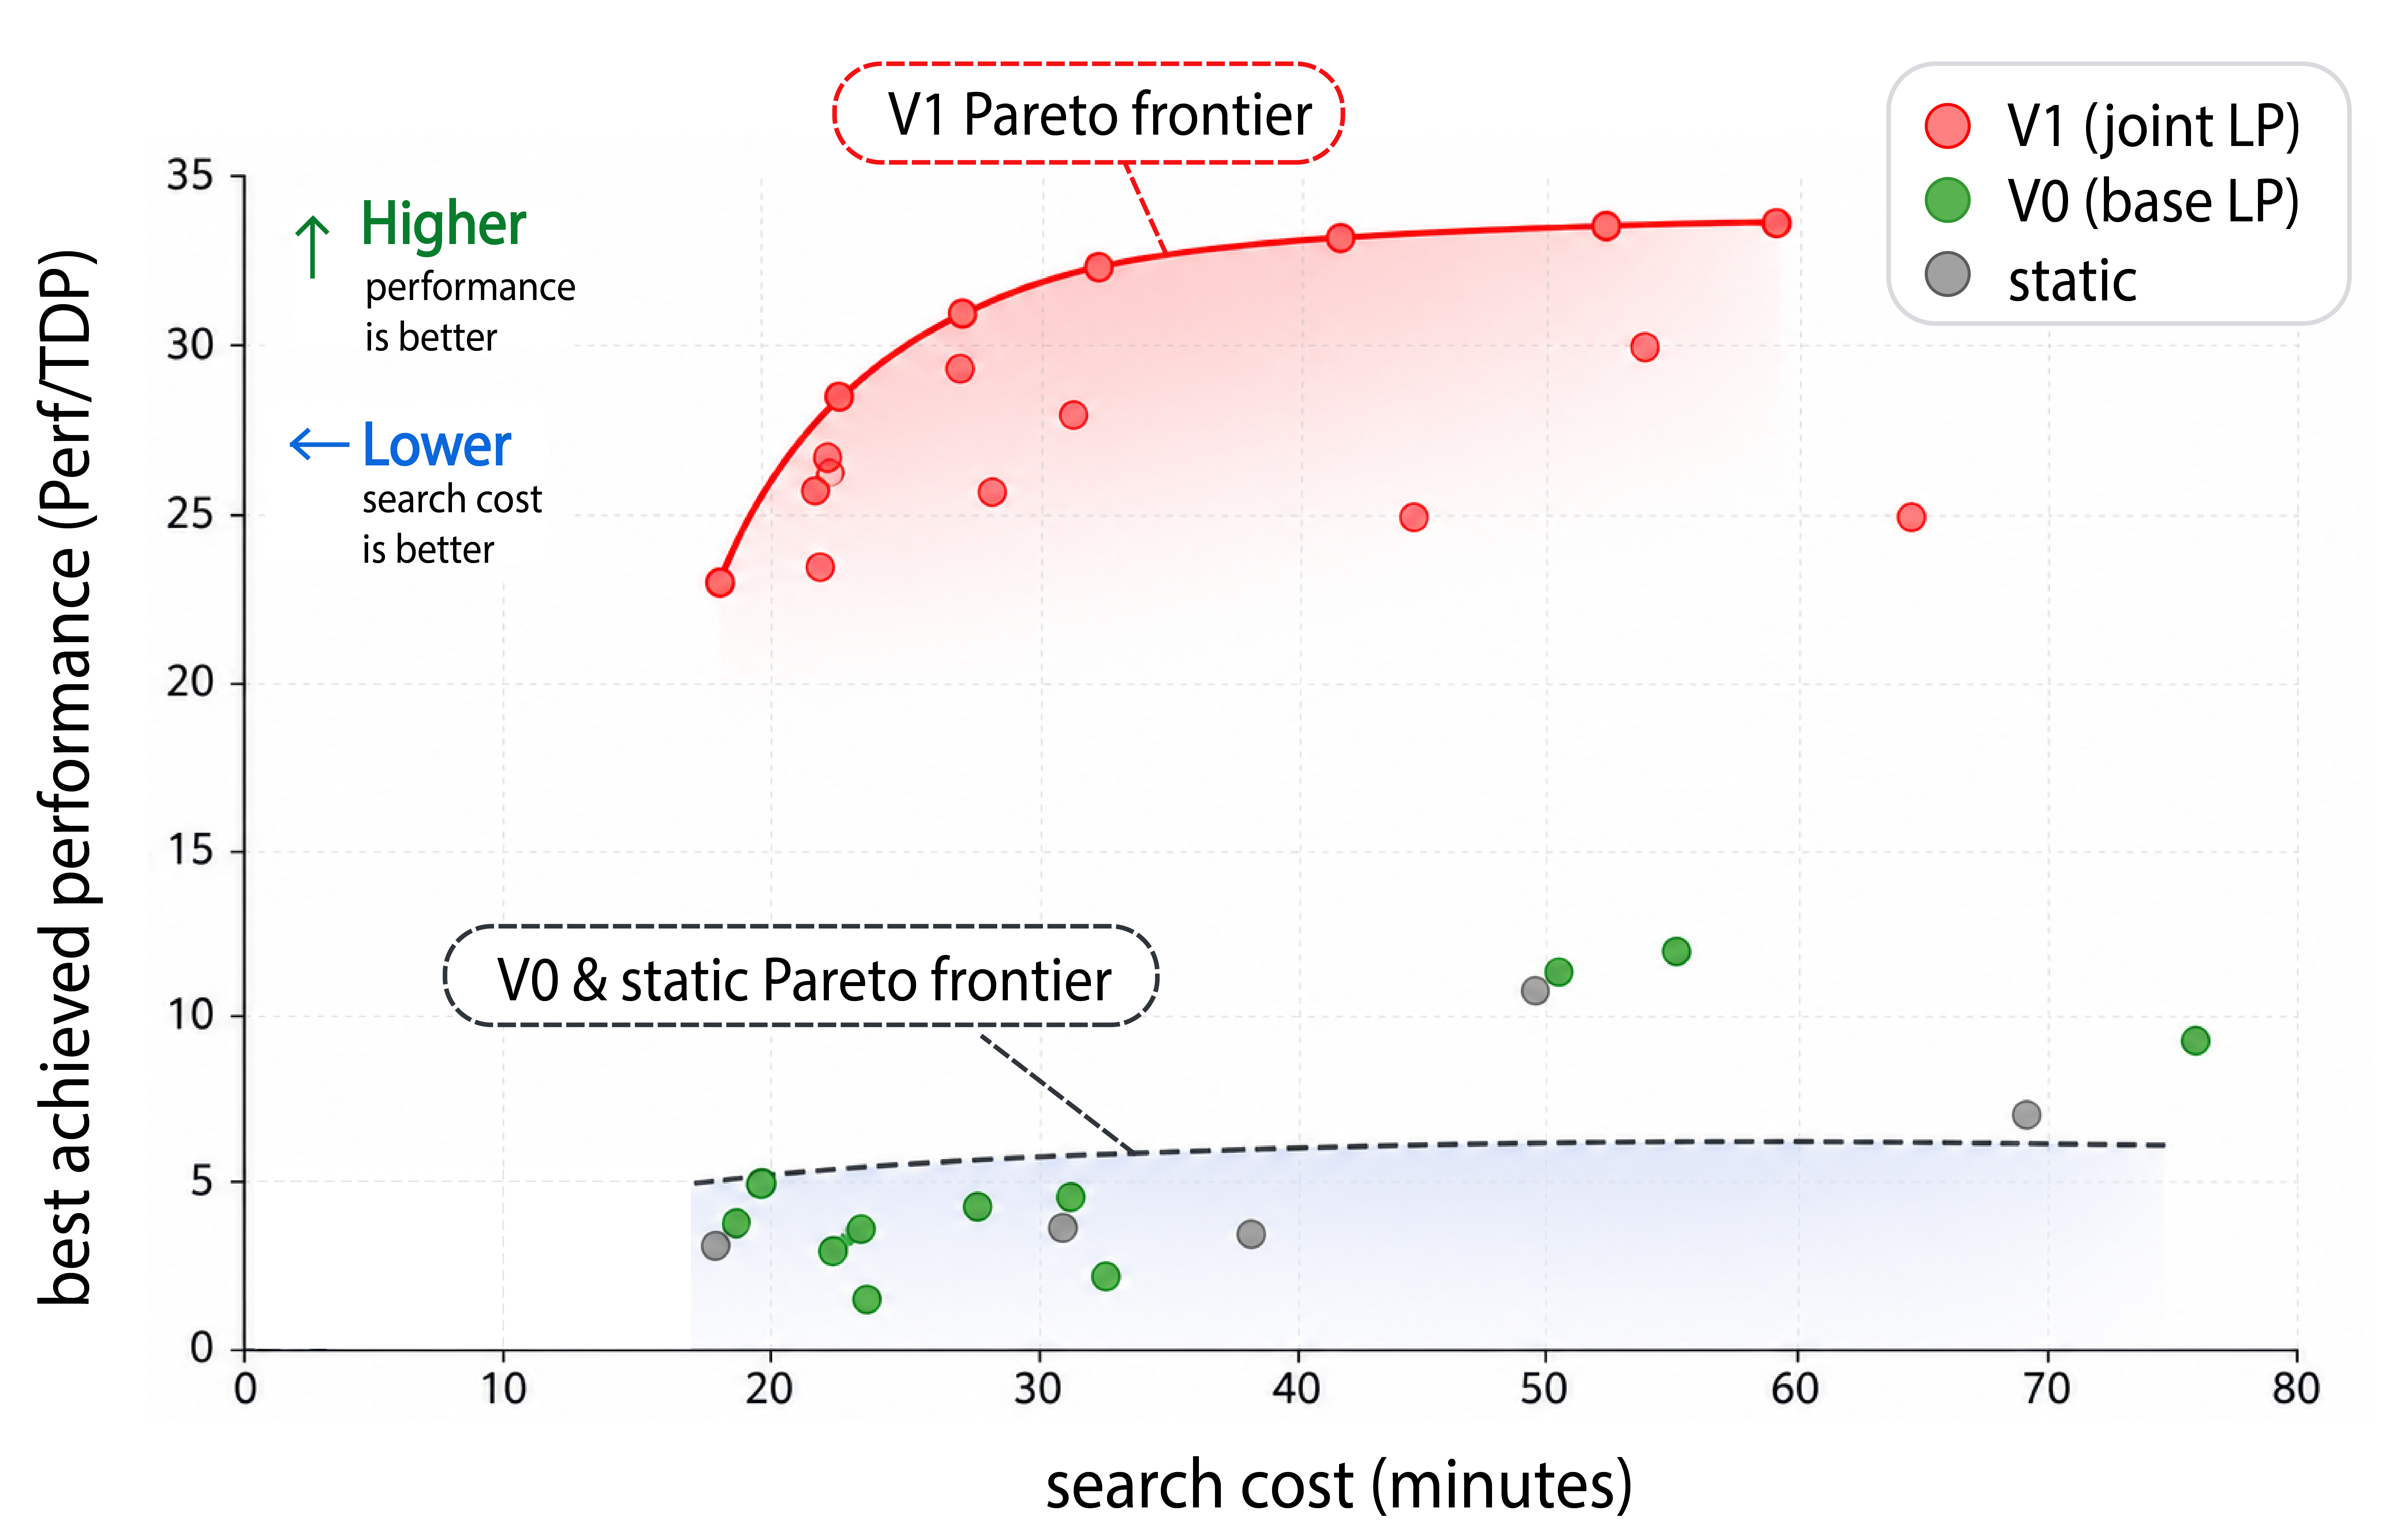
\includegraphics[width=0.7\linewidth]{figs/pareto_v2.png}
% %     \caption{pareto frontier plot}
% % \end{figure}
% \begin{figure}[ht!]
%     \centering
% 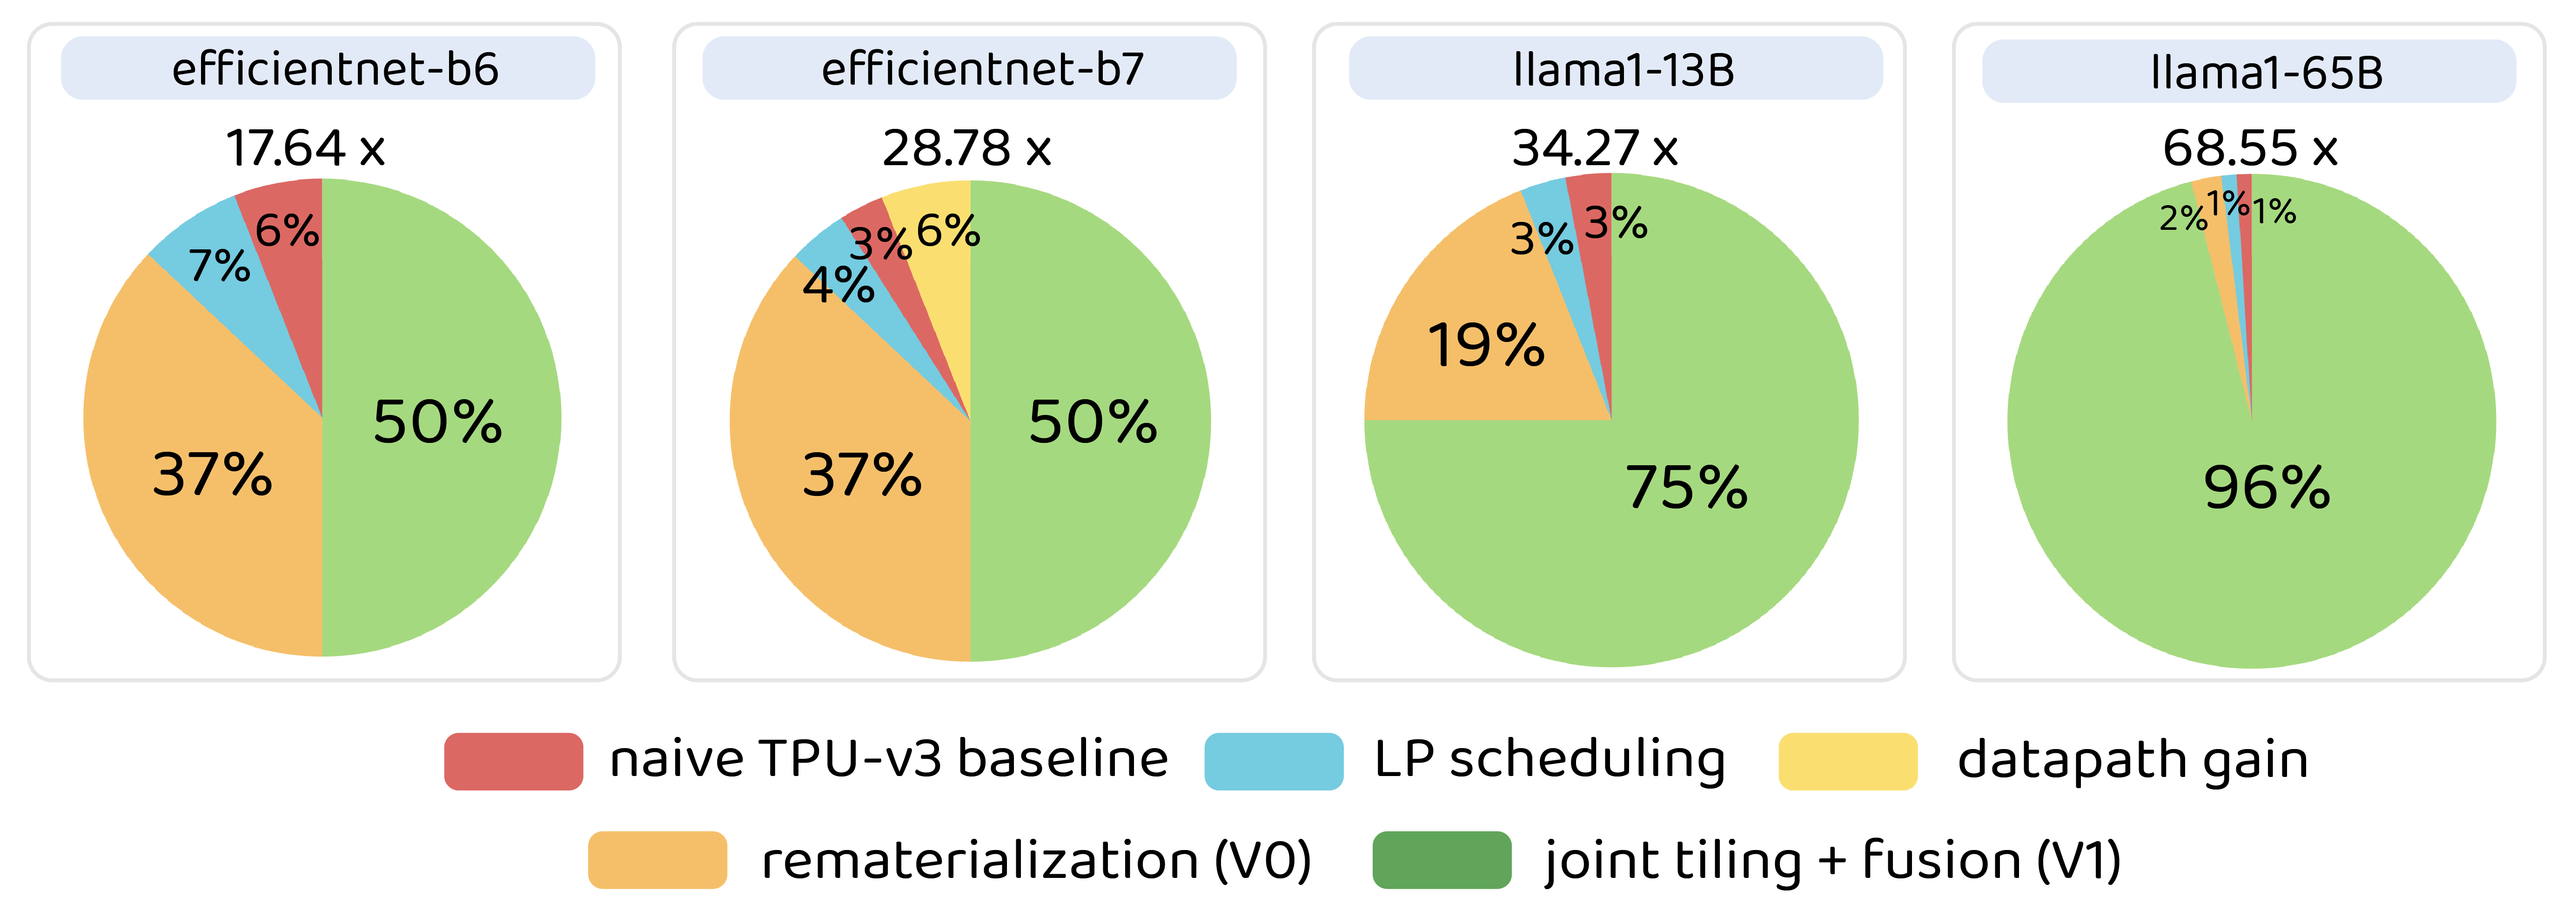
\includegraphics[width=0.85\linewidth]{fig3/speedup_decomposition_final_v2.png}
% \caption{Speedup decomposition over naive TPU-v3 baseline. Each pie shows the 
% relative contribution of four optimization sources to the total speedup. CHEETAH-V1 joint tiling + fusion dominates on all workloads, 
% especially on larger models where memory management is the primary bottleneck.}\label{fig:accel_decompose}
% \end{figure}
% \paragraph{CHEETAH-V0 vs.\ CHEETAH-V1 Unlock Progressive Gains.} Figure~\ref{fig:accel_decompose} decomposes the total speedup over a naive TPU-v3 baseline into four sources: LP-based scheduling and fusion, datapath gain from hardware search, dynamic rematerialization (CHEETAH-V0), and joint tiling + fusion (CHEETAH-V1).

% The dominant contributor across all workloads is V1's joint tiling-fusion 
% optimization. On EfficientNet-B1, V1 accounts for 50\% of total speedup, 
% with LP scheduling (28\%) and datapath gain (22\%) splitting the remainder---and 
% no rematerialization benefit, consistent with B1's small activation footprint 
% fitting comfortably in Global Memory. B3--B4 show a similar 50\% V1 share, but 
% V0 rematerialization now contributes 25\%, reflecting the growing value of 
% recomputing large depthwise activations rather than reloading them from DRAM. 
% From B5 onward, V1's share rises sharply to 75--88\%, as the increasing 
% model size makes joint tiling-fusion the primary lever: memory management 
% dominates, and the remaining sources (LP scheduling, V0, datapath) each shrink 
% to single-digit percentages. The same pattern holds on Llama, where V1 accounts 
% for 83--87\% of the total speedup.

% % \begin{wrapfigure}{r}{0.48\textwidth}
% %     \centering
% %     \vspace{-12pt}
% %     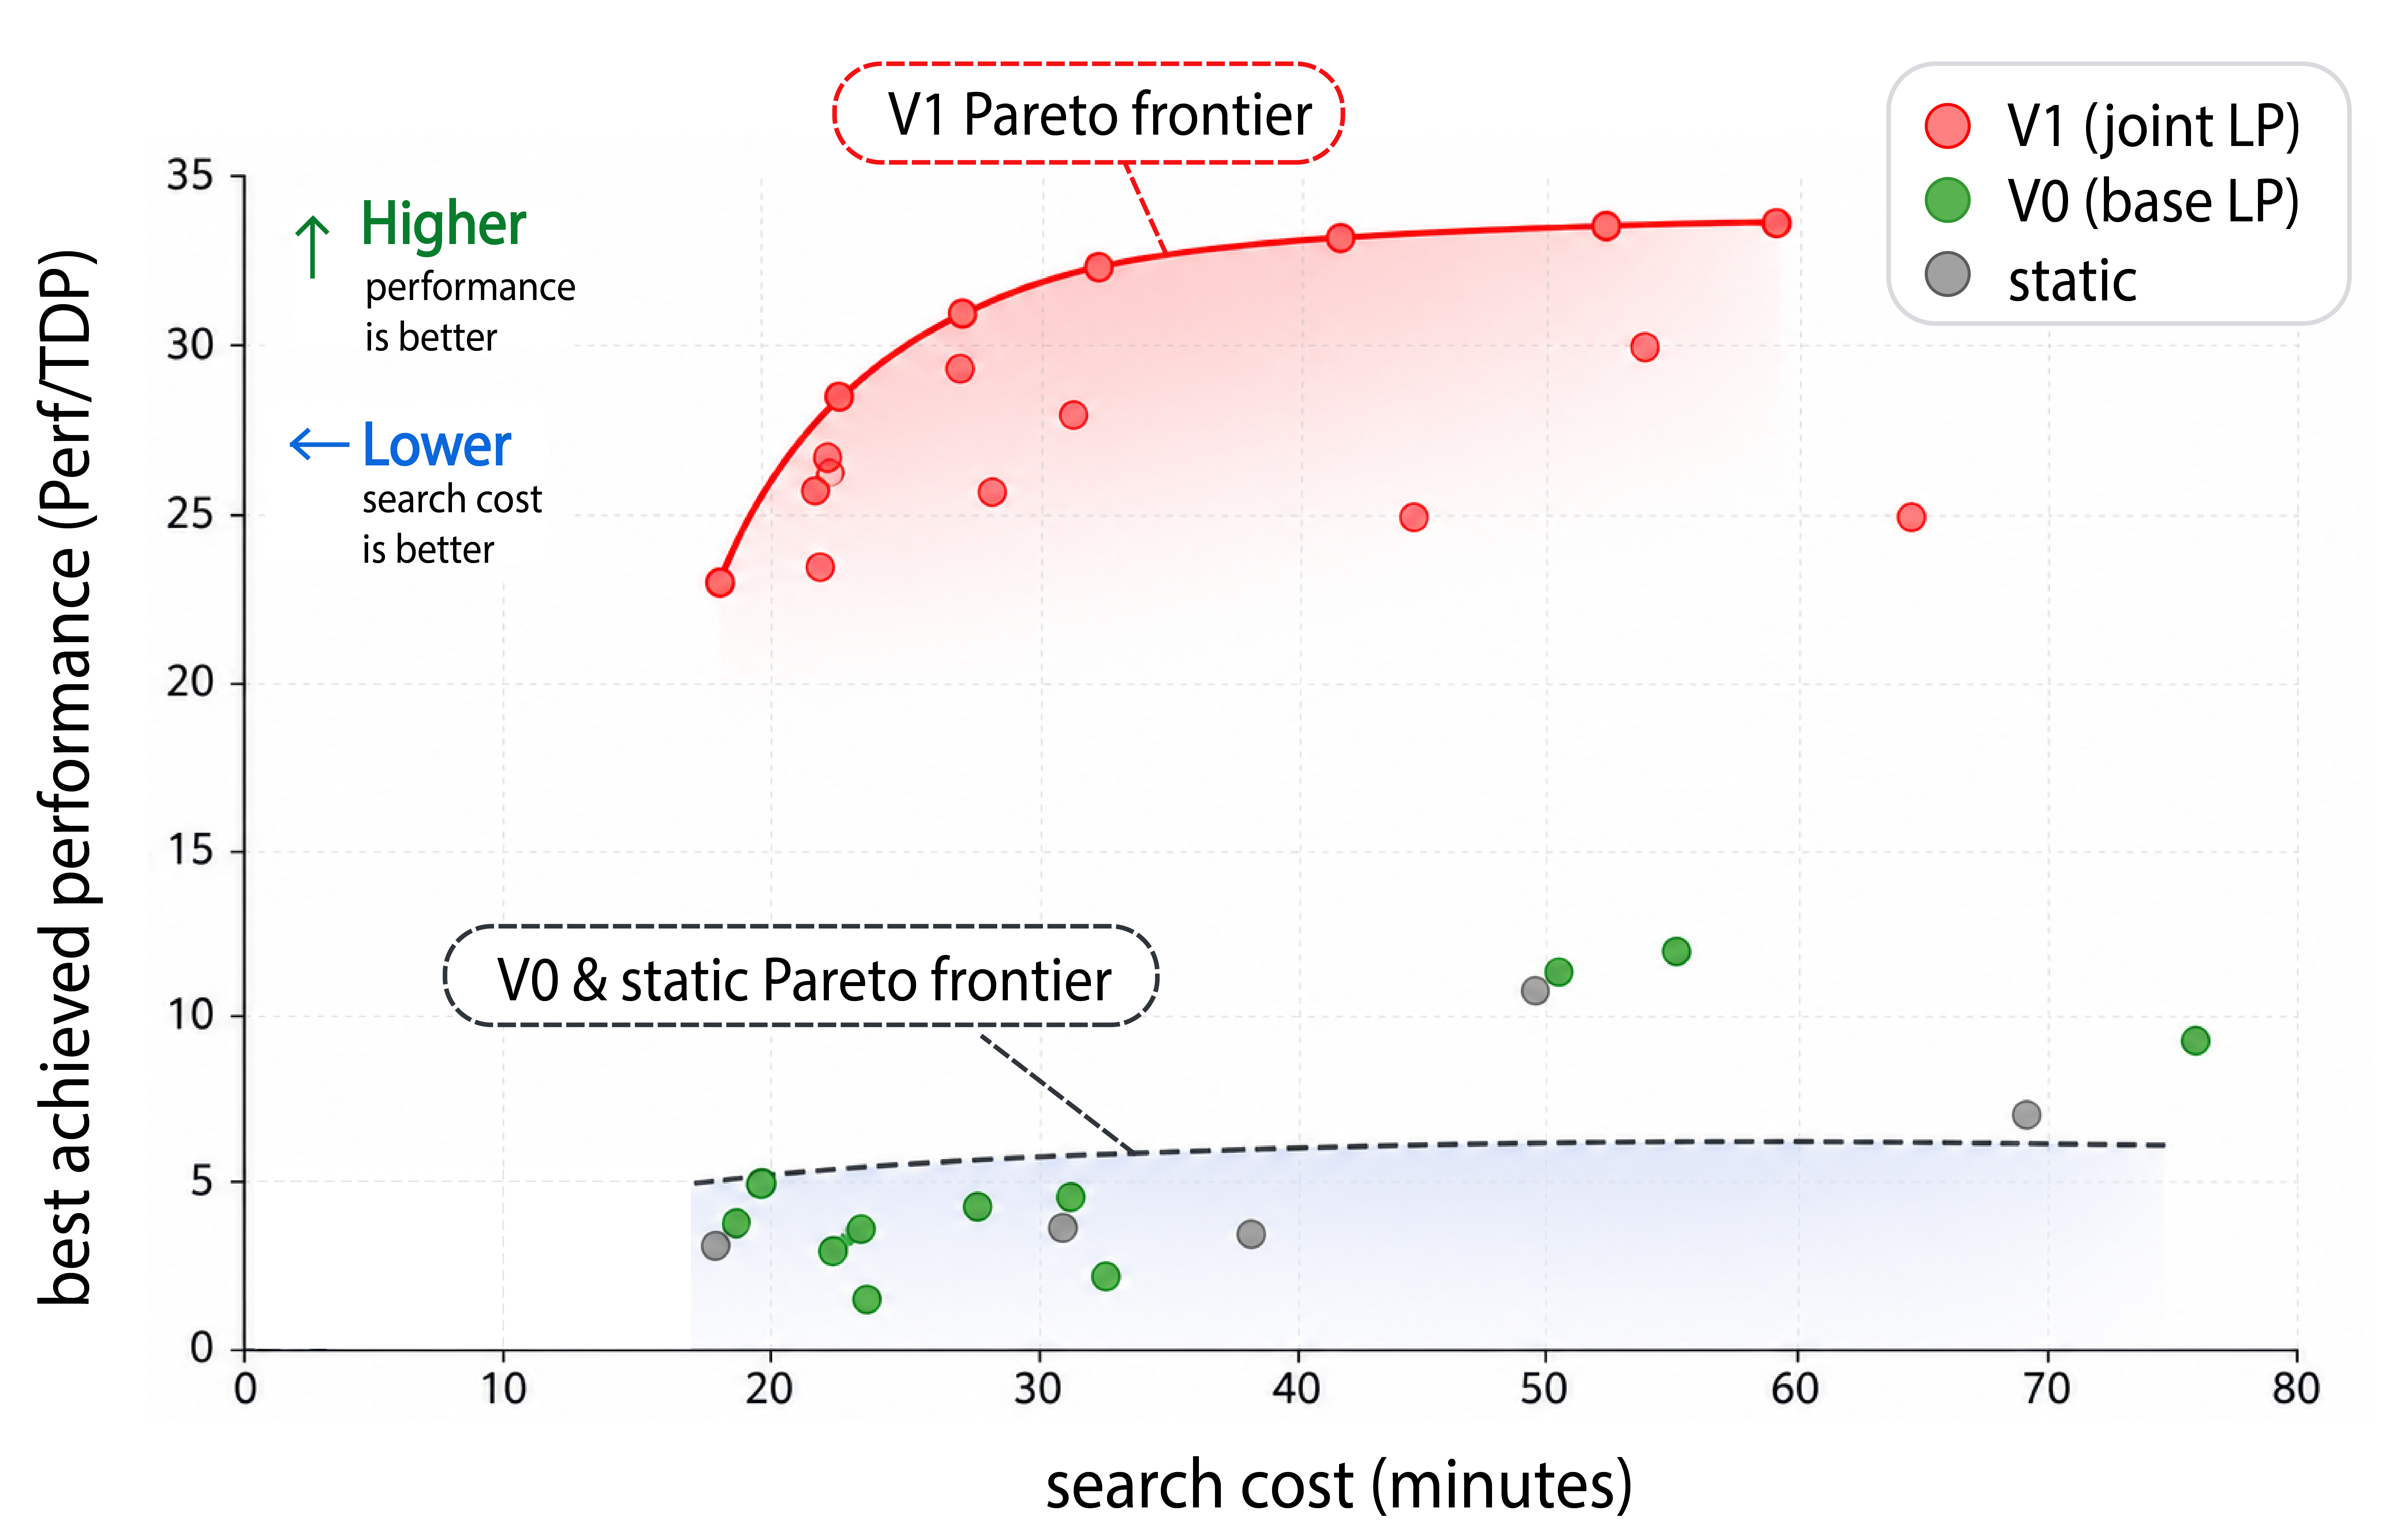
\includegraphics[width=0.48\textwidth]{figs/pareto_v2.png}
% %     \vspace{-18pt}
% %     \caption{Search cost vs.\ Perf/TDP Pareto frontier. V1 dominates V0 and static across all time budgets.}
% %     \label{fig:pareto}
% %     \vspace{-10pt}
% % \end{wrapfigure}

% Critically, Figure~\ref{fig:speedup} shows static fusion method is \emph{infeasible} on modern large models (Llama-70B, and DeepSeek-V3), because their large activation tensors cannot fit under a static pinning policy. The V0 formulation resolves feasibility for on large models via dynamic placement but remains time-intensive for a small number of 50 trials: measuring 58.42 hours on Llama-70B and 69.39 hours on DeepSeek-V3 (Figure~\ref{fig:wallclock}). In contrast Figures~\ref{fig:wallclock} and ~\ref{fig:speedup}, show the CHEETAH-V1 formulation out performs comparitive strategies in terms of speedup against the TPU-V3 baseline, and require only 1.17 hours on Llama-70B and 2.17 hours on DeepSeekv3 for 50 trails---a ${\sim}93\%$ average reduction. The powerful joint formulation is able to select memory-efficient tiling configurations alongside placement, achieving feasibility across the entire workload suite, demonstrating that joint optimization is not merely an incremental improvement but a qualitative capability unlock for large-scale models.

% % This demonstrates that by exploiting structural invariance and GPU-accelerated mathematical optimization, CHEETAH-V1 reduces the end-to-end co-design search time from days to under 2.2 hours—a ${\sim}93\%$ average reduction—while discovering architectural points that deliver up to $35\times$ speedup over the TPU-v3 baseline.

% % Figure~\ref{fig:pareto} shows the Pareto frontier of best-achieved Perf/TDP versus wall-clock search cost. V1 strictly dominates both V0 and static at every time budget: within 10 minutes of search, V1 already exceeds the best Perf/TDP that V0 or static achieve after 60+ minutes. The V1 Pareto frontier reaches ${\sim}35\times$ Perf/TDP, roughly $3\times$ higher than the V0/static frontier at ${\sim}10\text{--}12\times$. This gap reflects two compounding advantages: V1 explores a strictly larger feasible region (joint tiling-fusion), and it eliminates Timeloop from the per-trial critical path, allowing more trials within any fixed time budget.



% \paragraph{Practical insight.}
% Both LPs are extreme-aspect-ratio sparse: for \texttt{llama3\_70b},
% $m, n \sim 10^6$ and $\mathrm{nnz} \sim 5 \times 10^6$, giving roughly
% 1 nonzero per million matrix entries.
% The time-band structure means a coordinate-descent or stochastic PDHG
% solver would converge in $\mathcal{O}(T)$ sweeps if bands were the only
% structure.
% The capacity rows in both V0 and V1 LP formulations are the sole feature breaking strict banded structure, and they are precisely what couples the schedule globally. This is the desired behavior of a memory-aware placement formulation.

% % \todo{Report LP solve times for V0 and V1 across all benchmarks. Compare wall-clock time per trial against FAST's SCIP-based ILP solver (20 min timeout). Report LP relaxation gap: how often do fractional solutions need integer rounding, and what is the quality loss from rounding?}

% \paragraph{Structural invariance.}
% For a fixed workload and LP formulation, the LP constraint matrix
% has an invariant sparsity pattern across trials: the row/column
% dimensions and nonzero locations are determined only by the model graph structure — layer count $L$, timestep count $T$, edge set $E$, and Pareto count $C$ — not by the hardware candidate.
% Vizier changes only numerical values such as cycle coefficients,
% memory-capacity bounds, bandwidth-scaled access costs, objective weights, and TDP/area parameters. 
% This invariance allows us to reuse the same sparse matrix structure,
% variable ordering, block layout, and JIT-compiled sparse kernels in our adapted JAX PDLP solver across all hardware trials for a given workload. We apply the same diagonal preconditioning pipeline
% on each trial: a structural presolve with 20 log-geomean Ruiz iterations, followed by the PDLP preprocessing stack with 10 infinity-norm Ruiz iterations and one Pock--Chambolle $\ell_1$-scaling pass. This two-stage diagonal scaling handles the mixed coefficient magnitudes present in V0/V1 matrices — large byte-valued capacity rows together with $\pm 1$ persistence rows — without requiring a fragile matrix factorization. In production, this preconditioning pipeline is reused structurally across trials, recomputes only cheap diagonal scalings, finishes in under one second for matrices with approximately $5 \times 10^6$ nonzeros, and avoids factorization failures entirely because it consists only of $D_1 A D_2$ arithmetic.

% \paragraph{LLM Architect vs.\ Optimizer.} 
% \begin{wrapfigure}{r}{0.50\textwidth}
%     \centering
%     \vspace{-6pt}
%     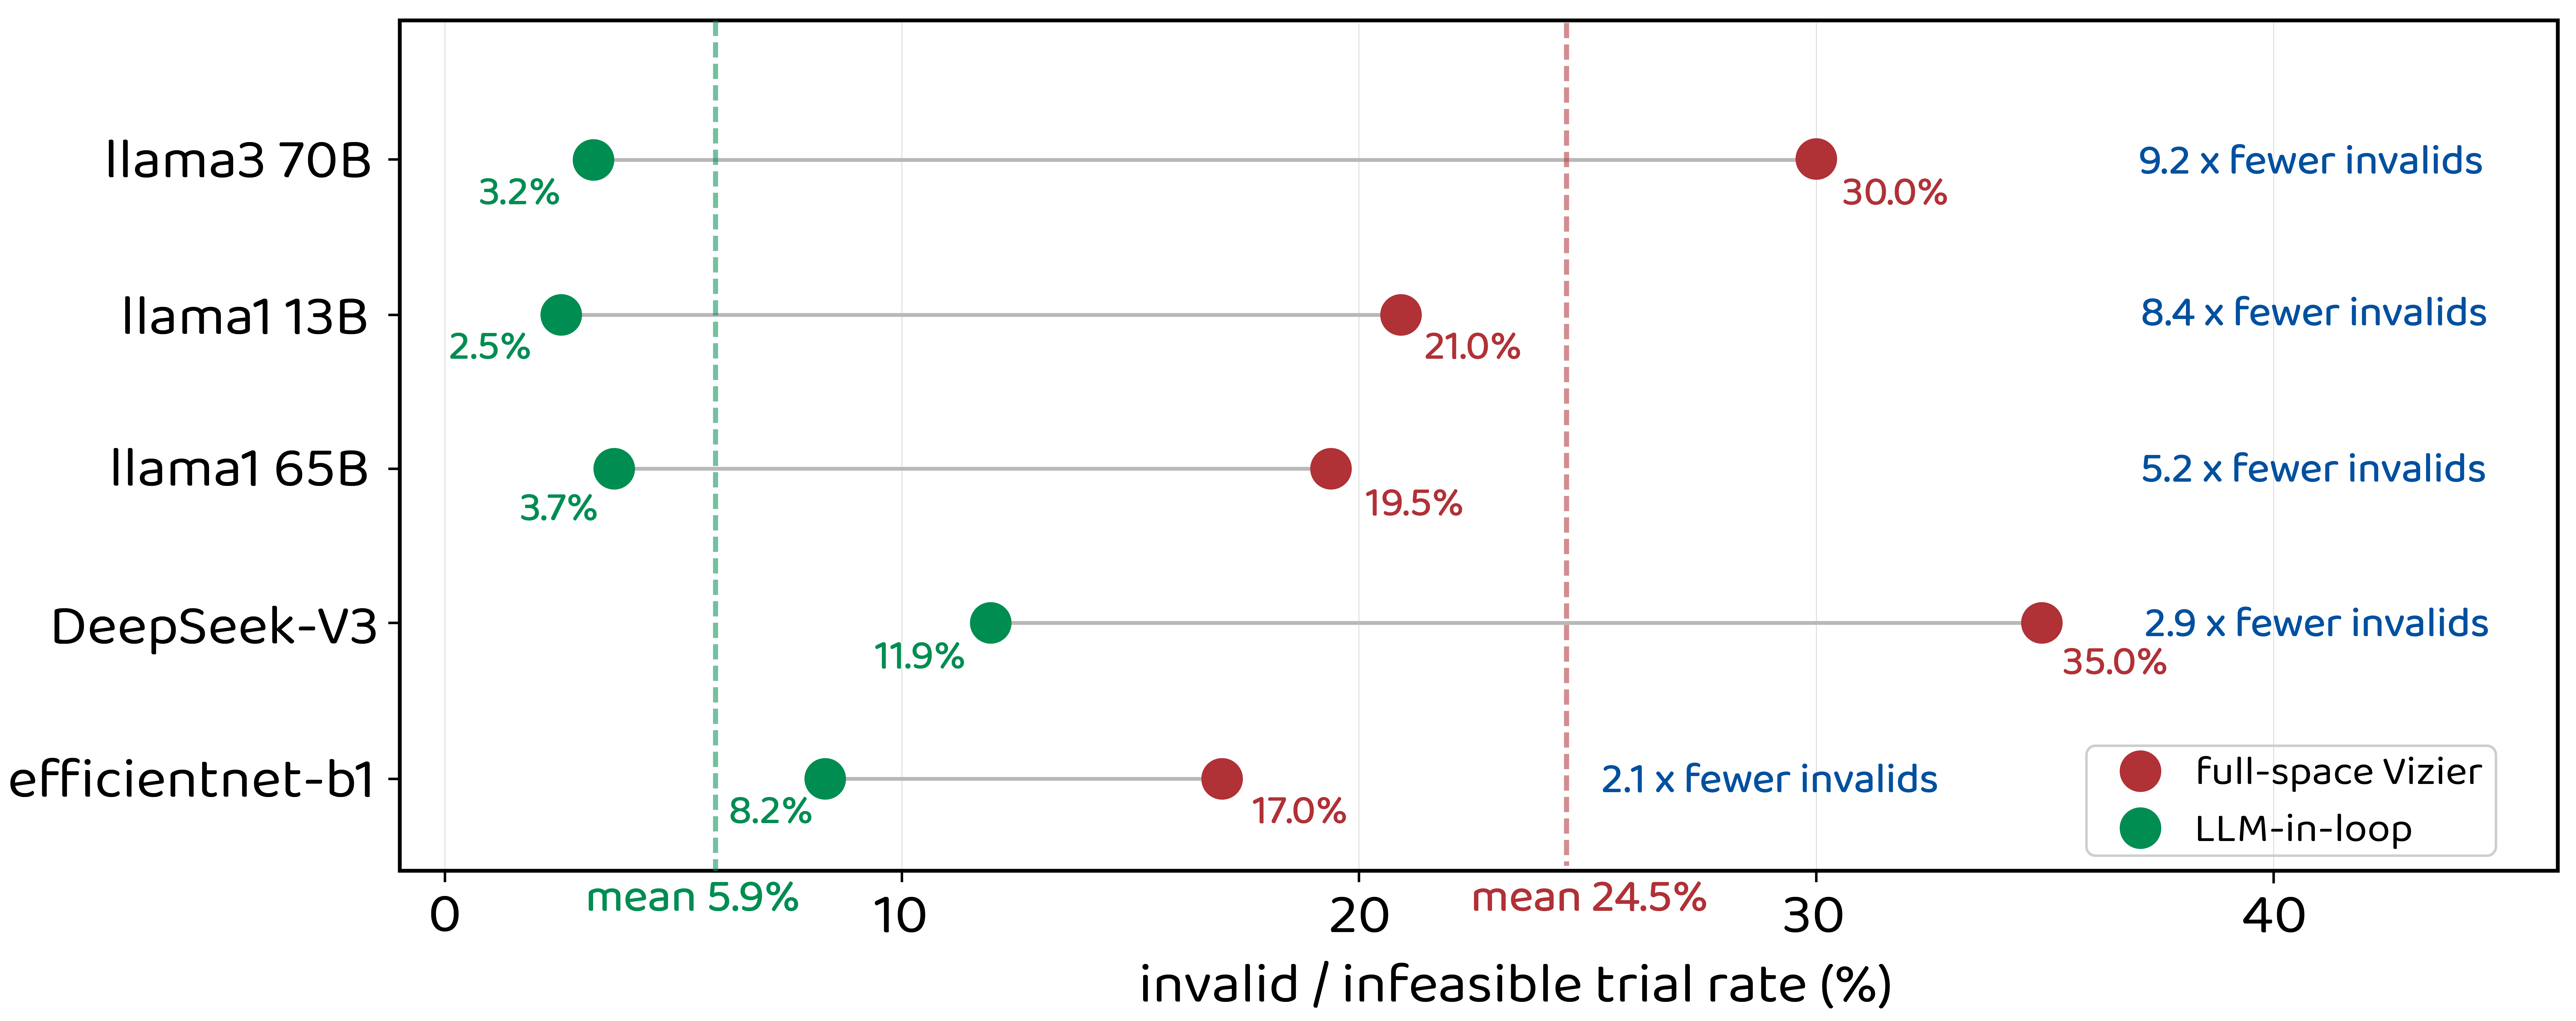
\includegraphics[width=0.48\textwidth]{fig3/llm_guide_v1.png}
%     \caption{Strategic Intelligence vs.\ Stochastic Brute Force. Green indicates the LLM-Architect has less wasted trials.}
%     \label{fig:llm}
%     \vspace{-10pt}
% \end{wrapfigure}

% Modelled on SkyDiscovery~\citep{skydiscover2026}, the LLM Architect prunes
% the outer search loop by proposing campaign patches rather than
% predicting raw performance. It analyses a Causal Ledger containing
% invalid rates, MFU, and solver diagnostics to suggest constrained
% hardware neighbourhoods for Vizier to explore locally. The V1 LP
% remains the ground-truth evaluator, supported by a Roofline Auditor
% that rejects physically impossible results.
% In a widened search space, the LLM loop reduces invalid evaluations
% from $24.5\%$ to $5.9\%$ on average — a $4.1\times$ reduction in wasted
% trials — while reaching the same optimal Perf/TDP scores as full-space
% Vizier. This demonstrates that the LLM's role is steering Bayesian
% optimisation toward feasible, workload-appropriate subspaces rather than
% replacing the solver. This framework establishes a foundation for
% integrating complex human reasoning into the co-design loop.

% % \subsubsection{LLM Architect vs. Optimizer}
% % The LLM Architect framework is modeled on SkyDiscover, and efficiently prunes the large outer hardware search loop by proposing campaign patches. Rather than predicting performance, the Architect reads a compact Causal Ledger containing invalid-rate history, MFU, roofline lower-bound checks, and LP diagnostics, then proposes a constrained hardware neighborhood for Vizier to search locally. The V1 LP remains the sole performance evaluator: for each candidate, it solves the joint tiling, fusion, placement, and rematerialization LP, while a deterministic Roofline Auditor rejects physically impossible results. In the widened V1 search space, all methods reach the same capped V1 Perf/TDP ceiling, so the key differentiator is search efficiency. The LLM loop reduces invalid hardware evaluations from 24.5\% under full-space Vizier to 5.9\% on average across five workloads, a 4.1× reduction in wasted trials, while preserving the same best V1 score. This shows that the LLM’s contribution is not replacing Vizier or the solver, but steering Bayesian optimization toward feasible, workload-appropriate architectural neighborhoods with far less wasted trials. This also sets the foundation for future work, where the LLM in the loop can adhere to follow more complex human reasoning signals.
% % \begin{figure}[ht!]
% %     \centering
% % 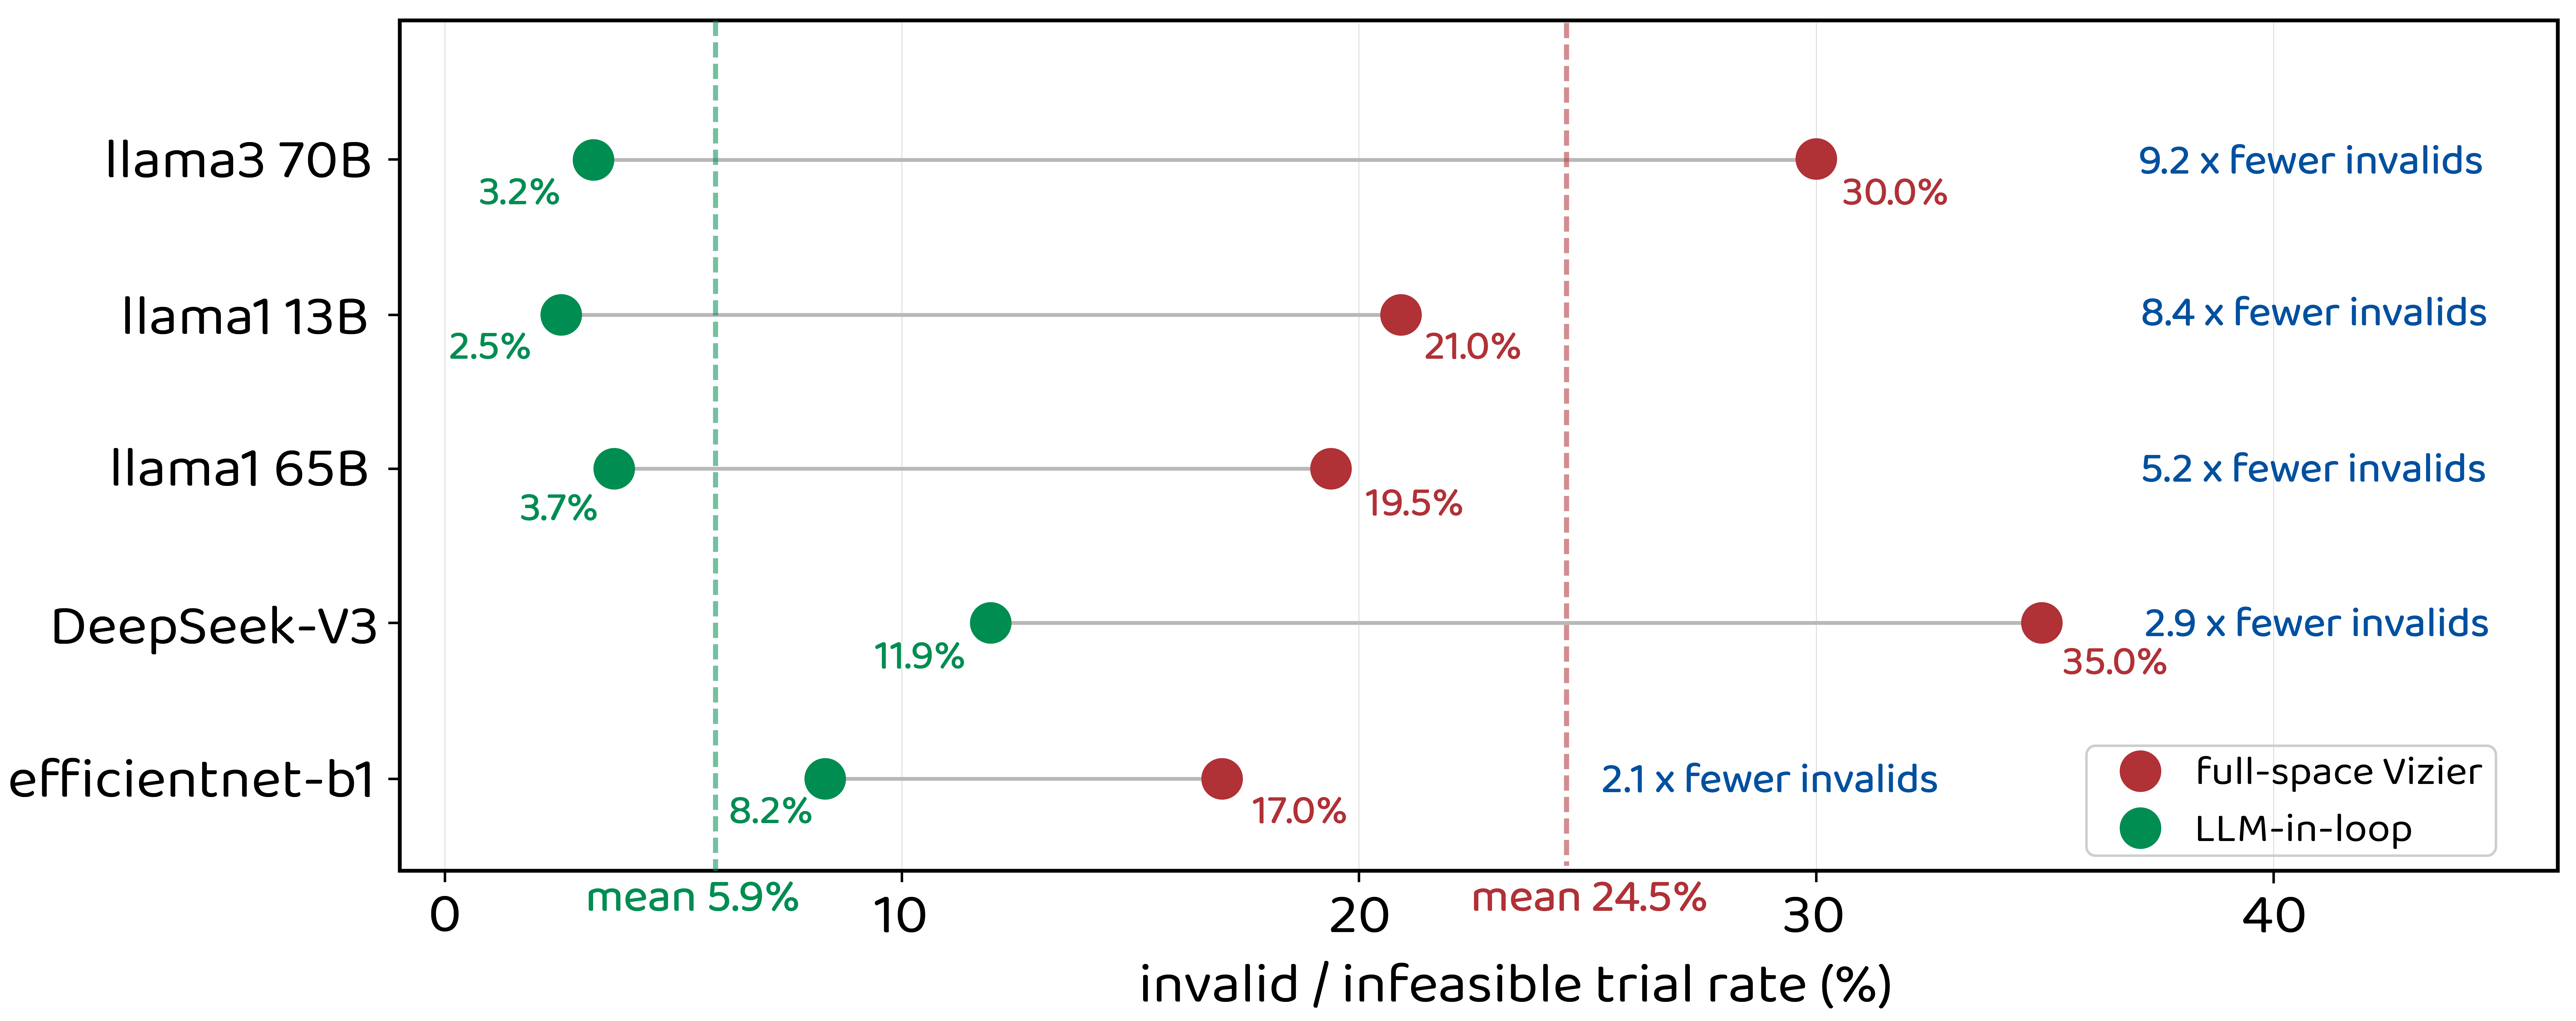
\includegraphics[width=0.85\linewidth]{fig3/llm_guide_v1.png}
% % \caption{Strategic Intelligence vs. Stochastic Brute Force}\label{fig:llm}
% % \end{figure}



% % The LLM should not just ask, “What chip has the best Perf/TDP?” We aim to answer the question “Given this user’s workload and deployment goal, what is the architectural region to search for this deployment task?”. Therefore we have the LLM emit profile-conditioned campaigns that take specific user inference tasks into consideration. For each $(\text{deployment profile},\ \text{workload})$ cell, we ran a
% % 200-trial LLM-Architect experiment using the same Qwen2.5-7B-Instruct + LoRA with differing user input profiles. At the start of each round, the prompt was assembled from a fixed system
% % prompt, the active deployment profile, three few-shot examples, and a per-round user message containing the workload, recent feedback signals, current search bounds, and the causal ledger.
% % The Strategist returned a one-line JSON campaign patch, which the
% % validator accepted only if it was a strict legal subset of the parent space, satisfied hard rules such as patch-volume $\leq 10\%$, ridgepoint and MAC/BW constraints, and avoided forbidden regions.

% % Thus, the experiment isolates whether the profile-conditioned LLM prompt alone can steer the same V1 evaluator toward different hardware families under different deployment intents.



% % \todo{Compare convergence rate of LLM-guided hardware search vs.\ Vizier-only (Bayesian, LCS, random baselines) in the style of FAST Figure~11. Report:
% % \begin{itemize}
% %     \item Number of trials to reach $X\%$ of best Perf/TDP found by 5,000-trial Vizier
% %     \item Quality of LLM-proposed configurations vs.\ Vizier-proposed configurations
% %     \item Qualitative analysis of LLM reasoning about hardware bottlenecks
% % \end{itemize}
% % }

% % \subsubsection{ROI Analysis}

% % \todo{Update FAST's ROI analysis (Table~4) with the improved Perf/TDP numbers from FAST-CORGI. Report deployment volumes required to reach 1$\times$, 2$\times$, 4$\times$ ROI targets. If Perf/TDP improvements are larger than FAST's, the break-even deployment volume should decrease correspondingly.}

% % \subsubsection{Pareto Frontier}

% % \todo{Plot the Perf/TDP vs.\ area Pareto frontier for V1-optimized designs compared to FAST and TPU-v3 baseline, analogous to FAST Figure~12.}

% page edit

% \section{Experiments}
% \label{sec:experiments}
% In all cases we use an adapted JAX PDLP solver for large models at LLama70-B and DeepSeekv3 scale across all three methods (Static, CHEETAH-V0, CHEETAH-V1); and use HiGHS as the default solver for all other smaller neural network models. In order to be consistent with prior work, our experimental results are presented as orders of speedup / performance against a vanilla TPU-V3. This is also since TPUs are targeted for NN accelerators (as opposed to GPUs), and the TPU-V3 has the most information publically released, making it possible for us to simluate it more accurately. 

% \subsection{Experimental Setup}

% \paragraph{Static Sequential Baseline.}
% We compare against the static optimization FAST framework using a simulated TPU-v3 baseline normalized to a sub-10nm process technology, following the same methodology as Zhang \etal. The baseline simulator is well-correlated with production hardware: on average within 8.2\,$\pm$\,2.7\% of profiled TPU-v3 performance. We evaluate against a \emph{simulated} TPU-v3 baseline to account for optimistic simulator assumptions.

% We evaluate across 11 representative workloads: EfficientNet-B1 through EfficientNet-B7, Llama13, 65, 70 models, and DeepSeek-V3-MoE. These workloads stress different parts of the hardware design space: EfficientNet stresses low-operational-intensity depthwise convolutions, while Llama and DeepSeek stress memory capacity, bandwidth, and large matrix operations. 

% \textbf{Single-workload specialization.} Each neural network workload is optimized independently. This experiment measures the best workload-specific hardware found under a fixed trial budget and identifies architectural preferences such as Global Memory size, bandwidth, MAC count, and systolic shape. In the case of Staitic and V0 methods, the pipeline involves: Vizier - Timeloop - LP solver. In the case of the V1 method, the pipeline is simplified to Vizier - LP solver. In each case we iterate for 100 trials per method x NN. 

% % \textbf{Fixed-hardware-workload generalization.} We search for general-purpose datapaths that perform well across the workload suite. The objective is a harmonic or geometric aggregation of per-workload Perf/TDP, forcing the search to balance CNN-style memory pressure and LLM-style compute/memory trade-offs.

% \textbf{LLM-Architect guides outer search.} We the LLM-guided outer-loop controller which proposes search-space interventions for Vizier. The advantage of the CHEETAH-V1 formulation is it removes dependence of Timeloop in the loop. Therefore the loop is reduced to just Vizier-LP solve, which dramatically speeds up the iterative process, thus permitting the LLM-Architect outer loop. The LLM is only permitted to change the search neighborhood of Vizier's input, the strict LP formulation on the inner loop does not change. This ensures mathematical and physical constraints are upheld in the space of co-design. 

% % \paragraph{Optimization framework.}
% % For the outer hardware search loop, we use Google Vizier with LCS optimization and safe search, running 100 trials per experiment (method X NN x Exp). Each trial invokes the LP solver for the inner optimization. The Static and V0 methods additionally have Timeloop in the loop (Vizier-Timeloop-LP solve). The advantage of the v1 formulation is it removes dependance of Timeloop in the loop. Therefore the loop is reduced to just Vizier-Lp solve, which dramatically speeds up the iterative process, thus permitted the Strategic LLM outer loop.

% We validate our framework through a multi-level audit process to ensure physical and numerical rigor.
% \textbf{Roofline Auditor.}
% A deterministic Roofline Auditor enforces physical feasibility by
% verifying that LP-predicted latencies never fall below the theoretical
% bound
% \begin{equation}
%     \mathrm{LB} = \max\!\left(t_{\mathrm{compute}},\;
%     t_{\mathrm{memory}}\right),
%     \label{eq:roofline_lb_val}
% \end{equation}
% where $t_{\mathrm{compute}}$ and $t_{\mathrm{memory}}$ represent the
% peak compute and memory bandwidth floors, respectively.
% All reported V0/V1 results are roofline-feasible with valid
% $\mathrm{MFU}_{\mathrm{bound}}$ and memory utilization metrics.

% \textbf{Campaign Validator.}
% A deterministic Campaign Validator legalizes LLM-proposed architectural
% neighbourhoods by enforcing hard hardware constraints — including TDP
% caps, area limits, and power-of-two parameter ranges — prior to Vizier
% sampling.

% \textbf{Causal Ledger.}
% A Causal Ledger tracks LLM interventions and observed outcomes,
% preventing redundant exploration of empirically invalid regions and
% ensuring full auditability of the search loop.

% \textbf{Solver Diagnostics.}
% We monitor solver diagnostics including primal/dual residuals, duality
% gap, and rounding gap. Designs are treated as trustworthy only when both
% the continuous LP relaxation and the rounded integer solution are
% numerically well-behaved.


% \subsection{Main Results}

% % \subsubsection{V0 vs.\ FAST Static Fusion}

% % \todo{Insert results table and figure comparing V0 (time-indexed placement + rematerialization) against FAST's static fusion ILP on all benchmarks. Key metrics: Perf/TDP improvement, fusion efficiency (\% of DRAM stall time eliminated), rematerialization frequency (how often does the solver choose to recompute rather than reload?).}

% % \paragraph{Expected findings.}
% % V0's dynamic placement should show the largest gains on workloads with: (1)~tight Global Memory budgets where static pinning wastes capacity on tensors that are only needed briefly, (2)~long dependency chains where tensor lifetimes vary substantially, and (3)~cheap-to-recompute operations with large activations (\eg, depthwise convolutions in EfficientNet).

% % \subsubsection{V1 vs.\ V0: Joint Tiling and Fusion}

% % \todo{Insert results table and figure comparing V1 against V0 on all benchmarks. Key metrics: Perf/TDP improvement, number of operations where V1 selects a different tiling configuration than Timeloop's greedy choice, and the resulting compute efficiency vs.\ fusion trade-off.}

% % \paragraph{Expected findings.}
% % V1 should show the largest gains on architectures with highly diverse layer types where a single tiling configuration cannot serve all operations well. EfficientNet (depthwise + pointwise convolutions with 100$\times$ variation in working-set sizes) and hybrid CNN-transformer models (convolutions + attention + MLP with fundamentally different compute-memory profiles) are expected to benefit most.


% % \subsubsection{stiatic vs v0 vs v1}
% % \begin{figure}[ht!]
% %     \centering
% %     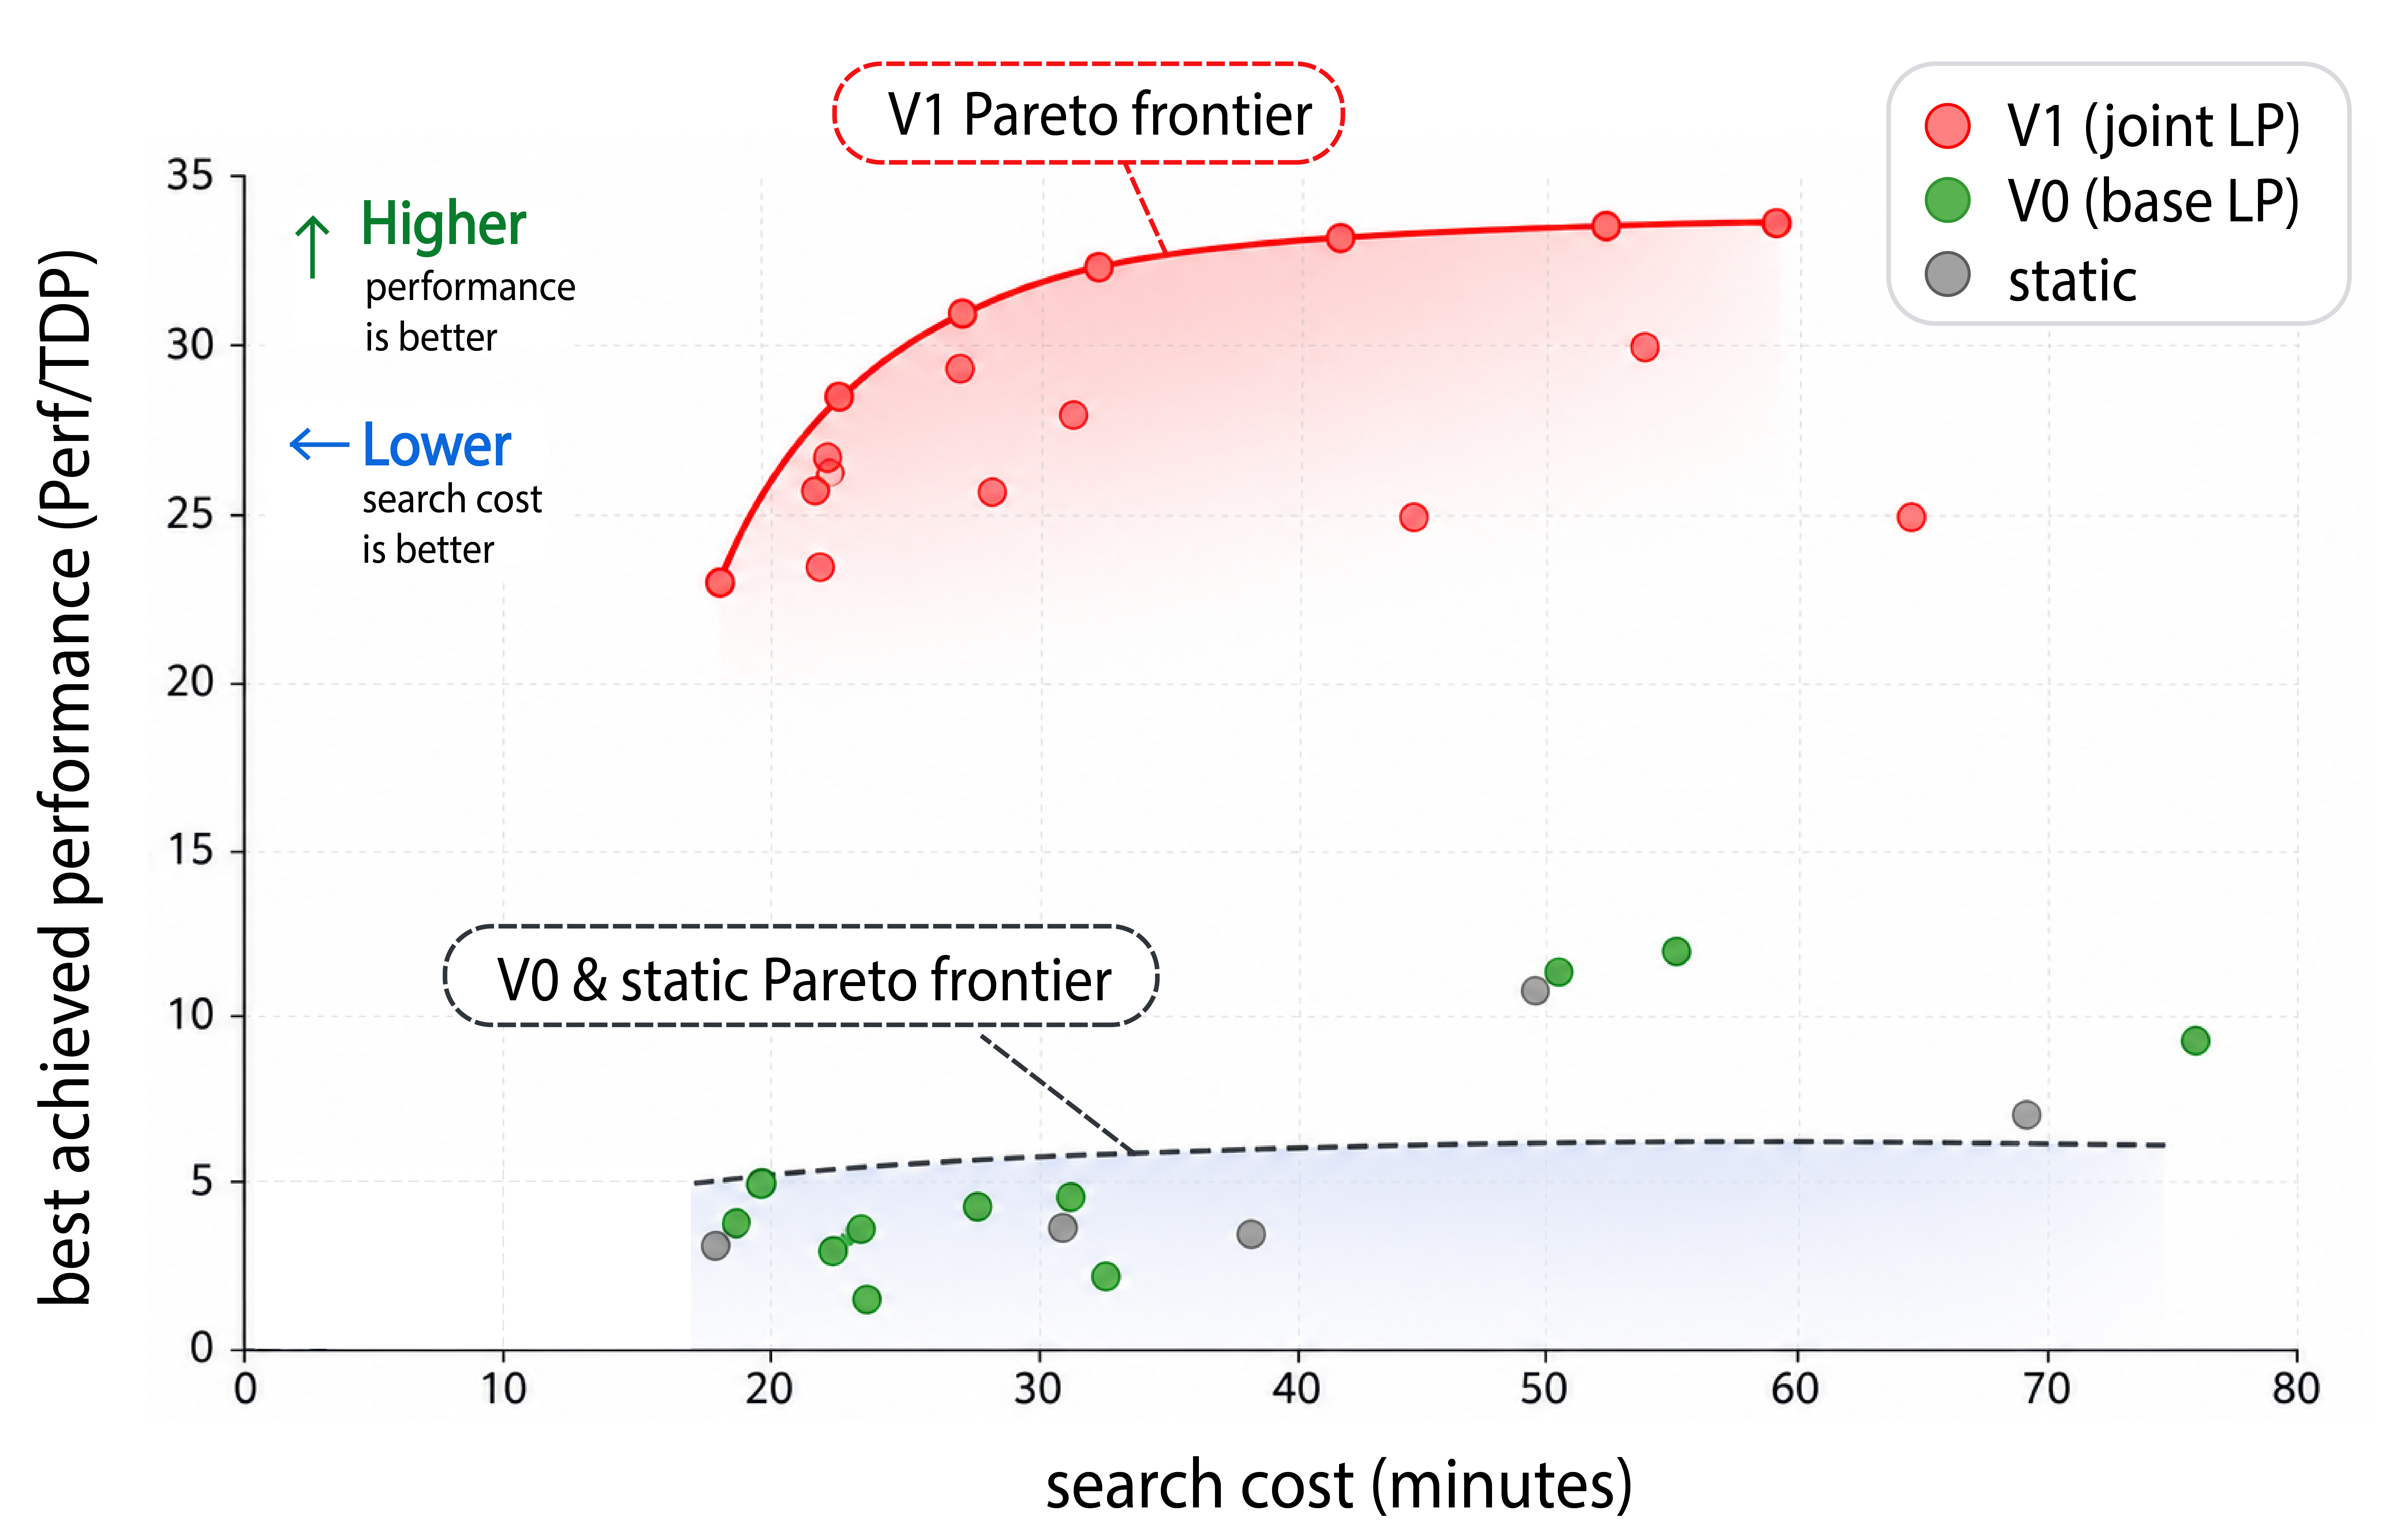
\includegraphics[width=0.7\linewidth]{figs/pareto_v2.png}
% %     \caption{pareto frontier plot}
% % \end{figure}
% \begin{figure}[ht!]
%     \centering
% 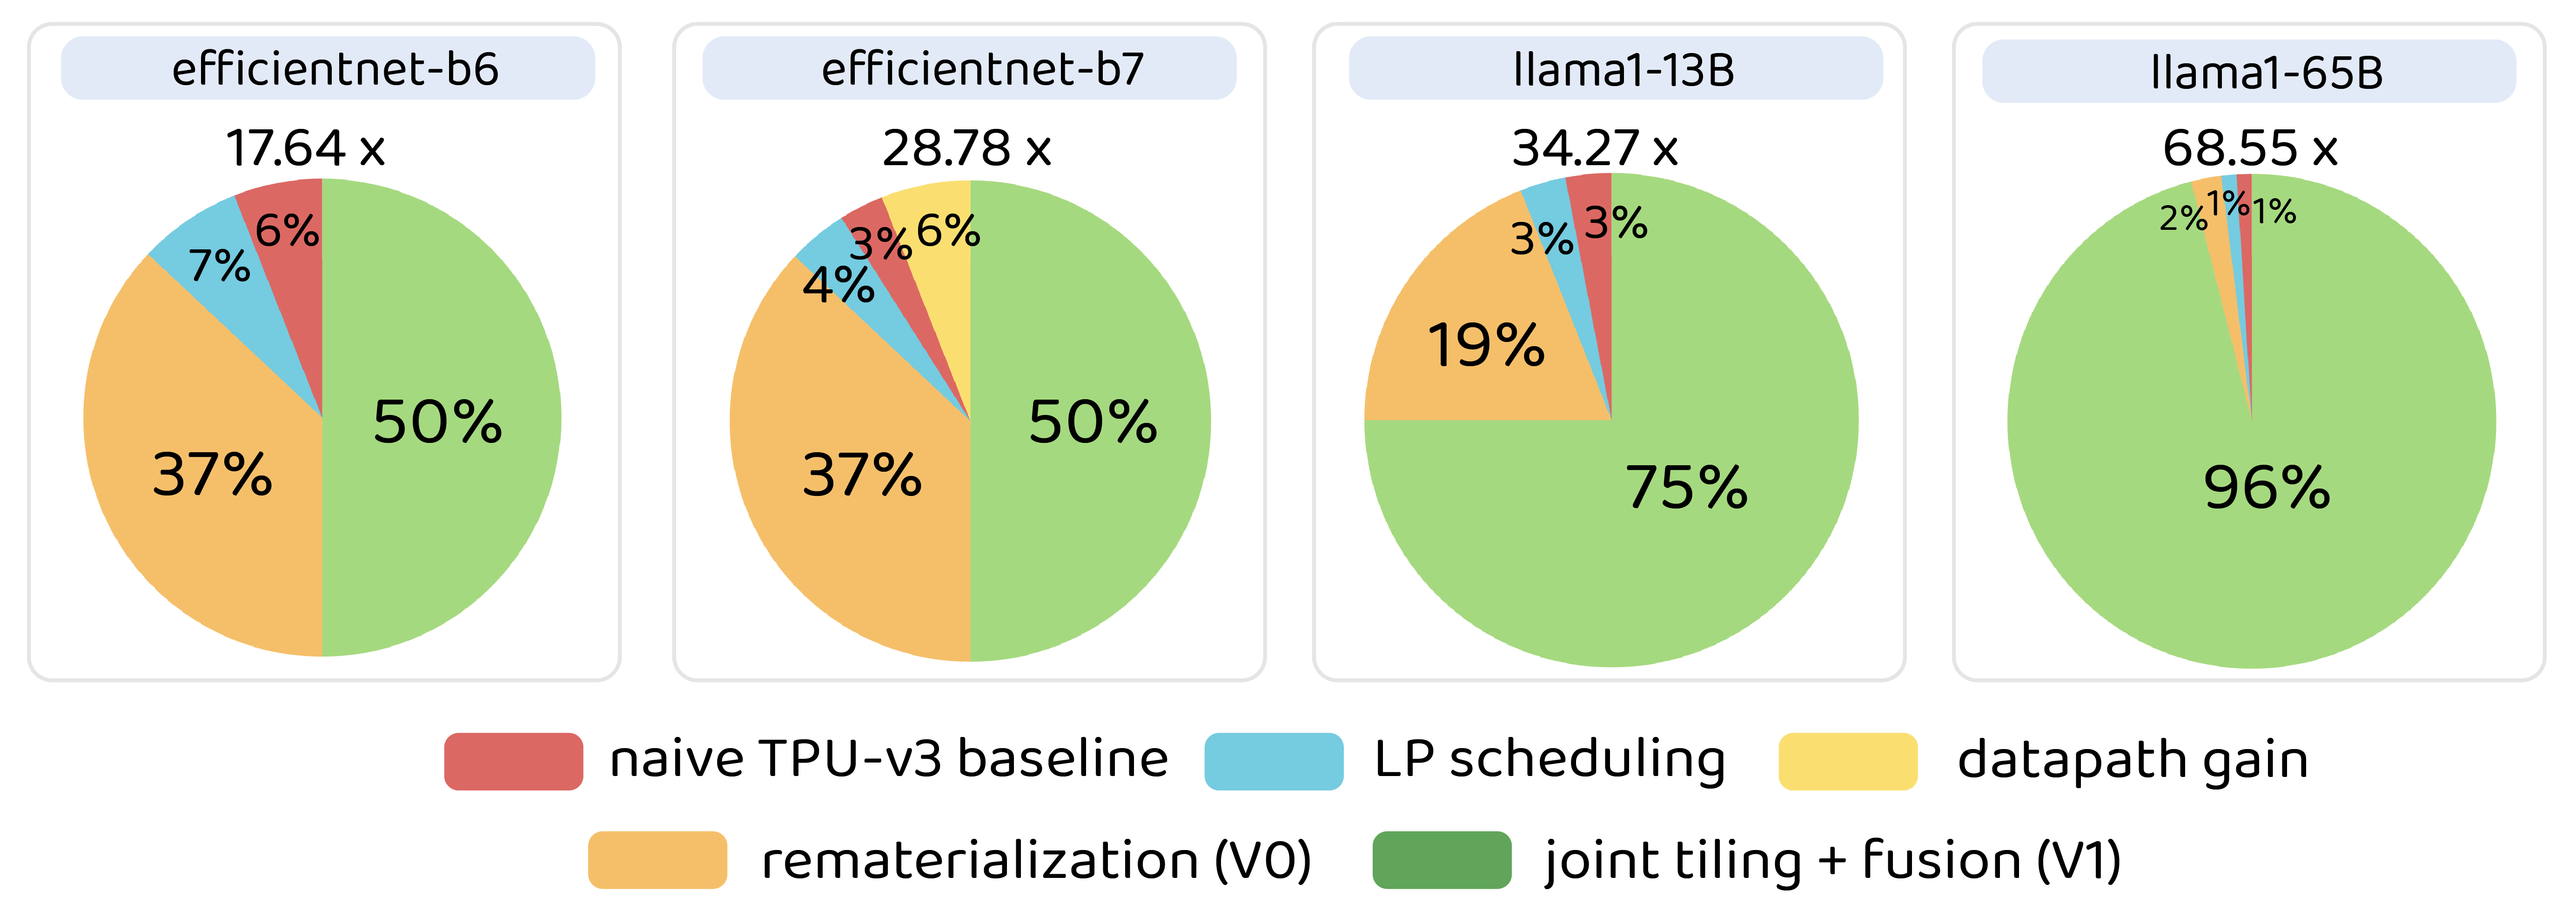
\includegraphics[width=0.85\linewidth]{fig3/speedup_decomposition_final_v2.png}
% \caption{Speedup decomposition over naive TPU-v3 baseline. Each pie shows the 
% relative contribution of four optimization sources to the total speedup. CHEETAH-V1 joint tiling + fusion dominates on all workloads, 
% especially on larger models where memory management is the primary bottleneck.}\label{fig:accel_decompose}
% \end{figure}
% \subsubsection{Static Baseline vs.\ CHEETAH-V0 vs.\ CHEETAH-V1 Unlock Progressive Gains}


% Figure~\ref{fig:accel_decompose} decomposes the total speedup over a naive TPU-v3 baseline into four sources: LP-based scheduling and fusion, datapath gain from hardware search, dynamic rematerialization (CHEETAH-V0), and joint tiling + fusion (CHEETAH-V1).

% The dominant contributor across all workloads is V1's joint tiling-fusion 
% optimization. On EfficientNet-B1, V1 accounts for 50\% of total speedup, 
% with LP scheduling (28\%) and datapath gain (22\%) splitting the remainder---and 
% no rematerialization benefit, consistent with B1's small activation footprint 
% fitting comfortably in Global Memory. B3--B4 show a similar 50\% V1 share, but 
% V0 rematerialization now contributes 25\%, reflecting the growing value of 
% recomputing large depthwise activations rather than reloading them from DRAM. 
% From B5 onward, V1's share rises sharply to 75--88\%, as the increasing 
% model size makes joint tiling-fusion the primary lever: memory management 
% dominates, and the remaining sources (LP scheduling, V0, datapath) each shrink 
% to single-digit percentages. The same pattern holds on Llama, where V1 accounts 
% for 83--87\% of the total speedup.

% % \begin{wrapfigure}{r}{0.48\textwidth}
% %     \centering
% %     \vspace{-12pt}
% %     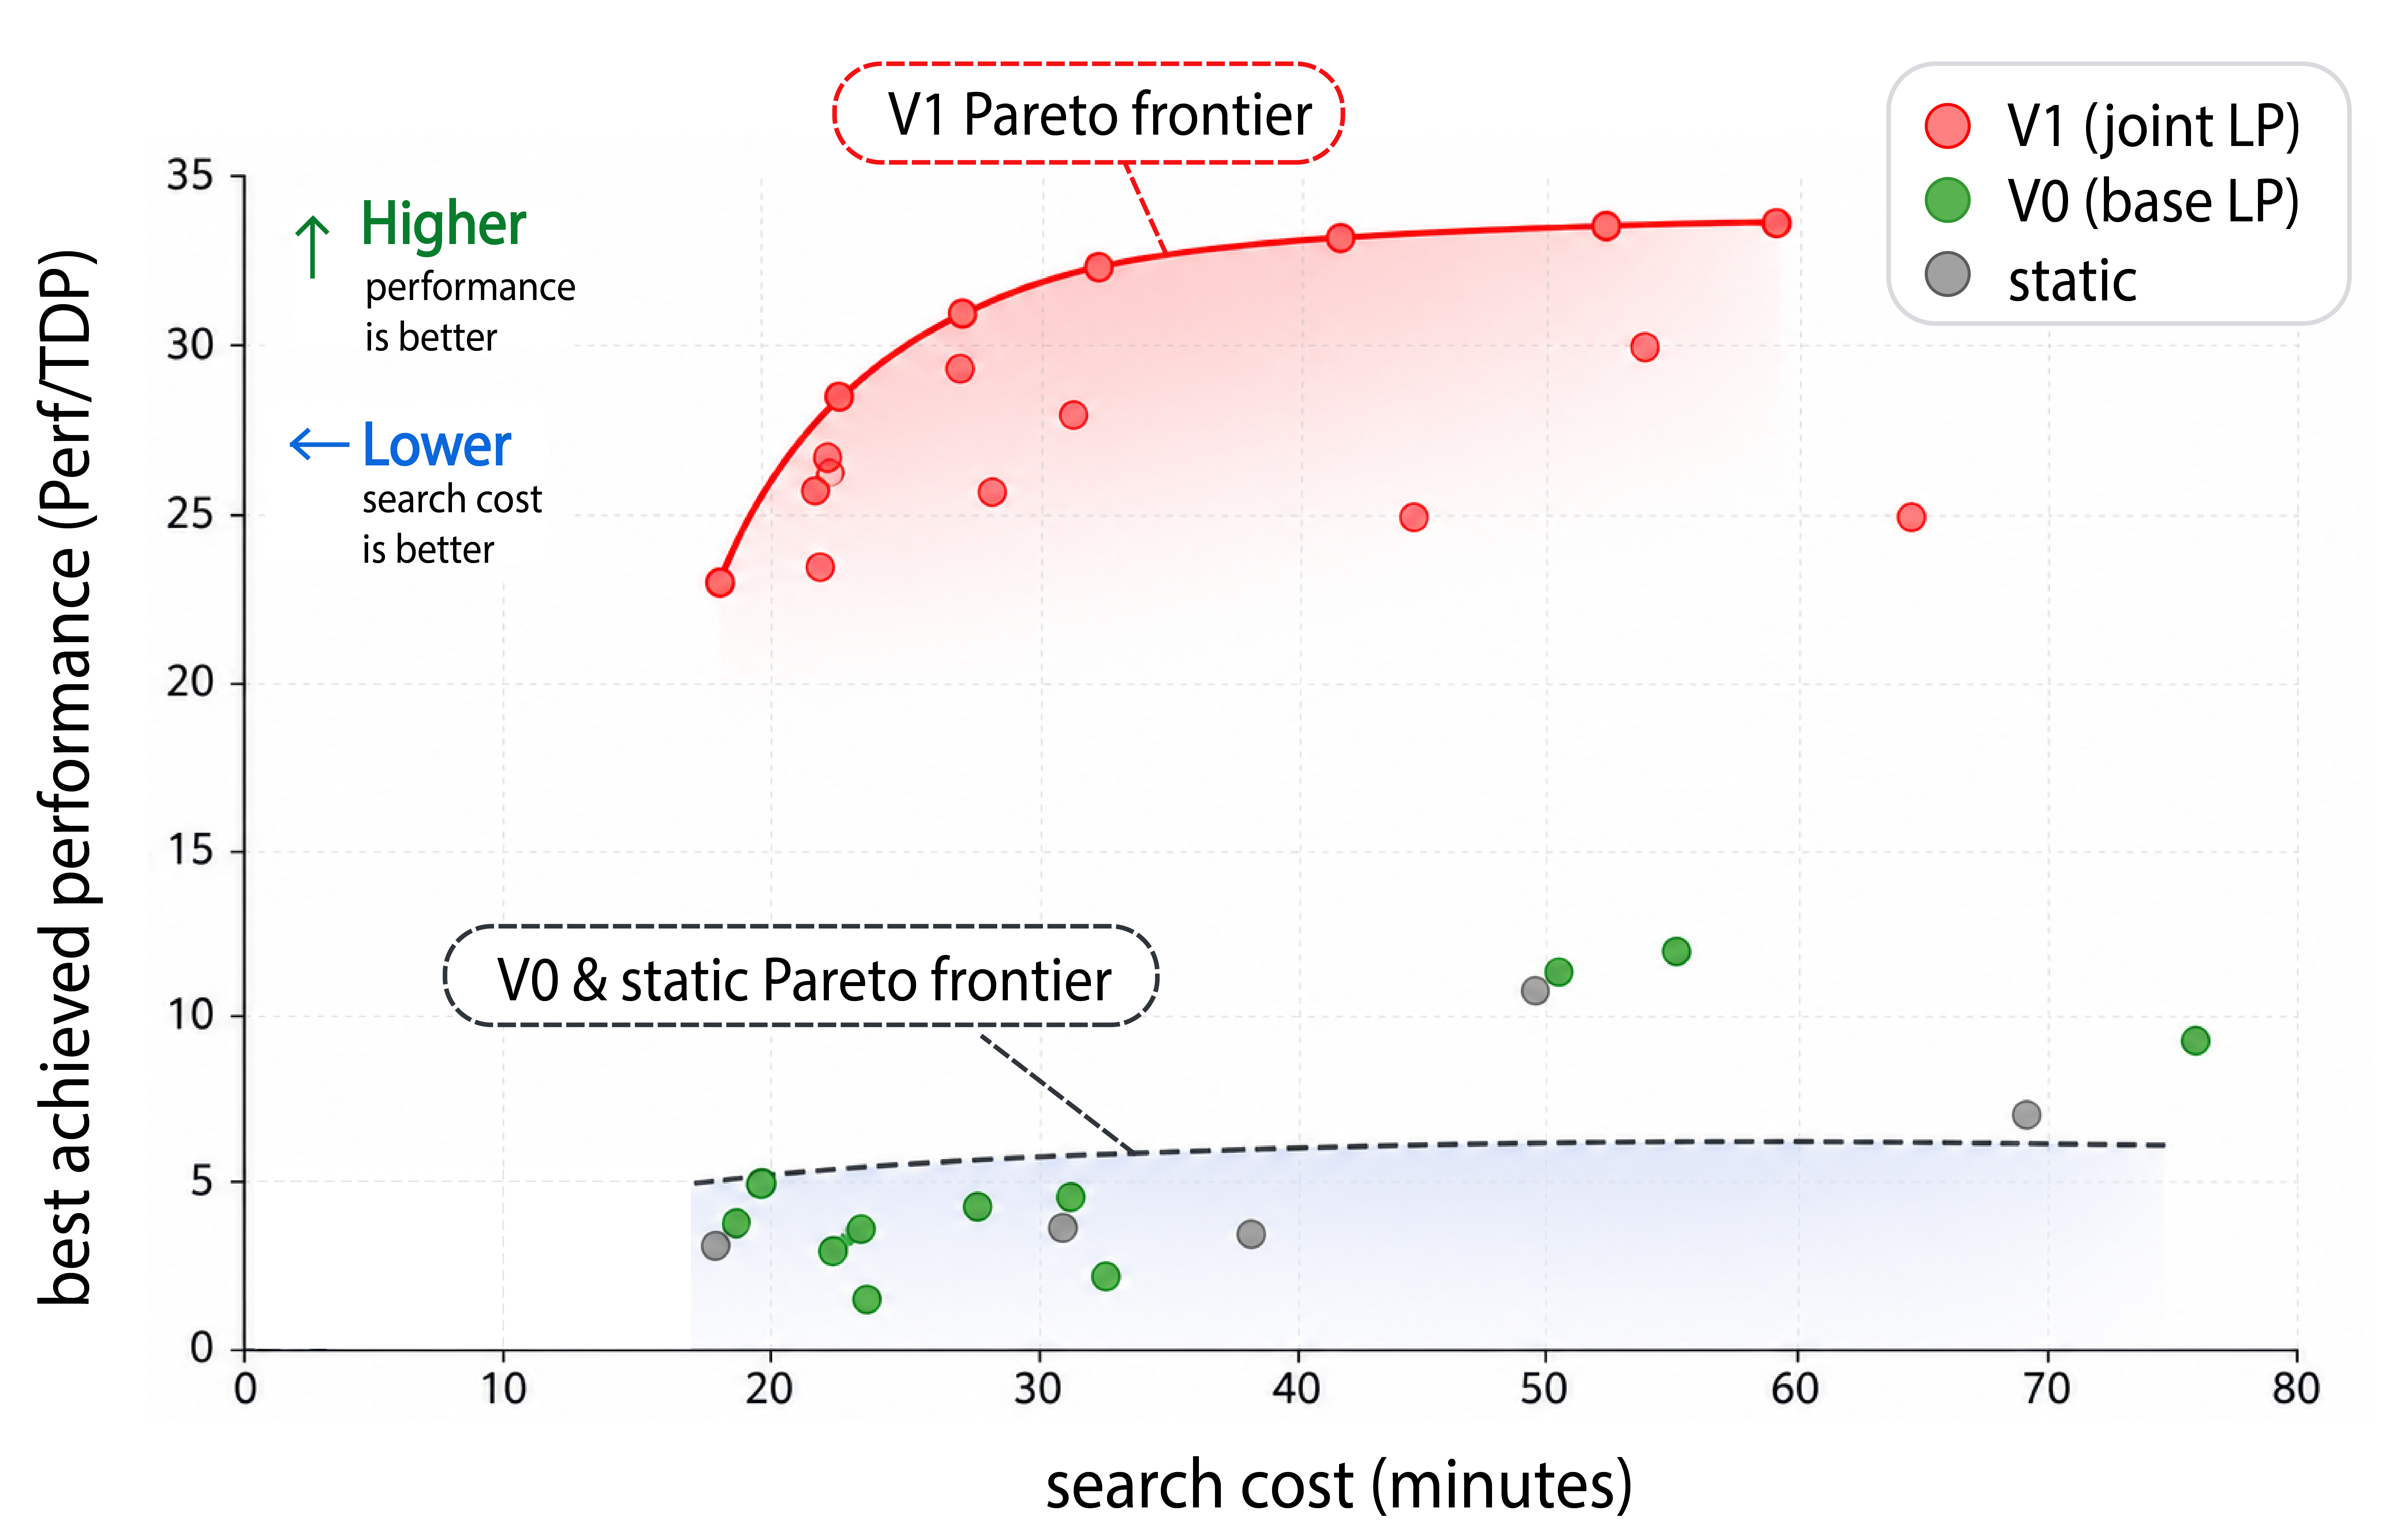
\includegraphics[width=0.48\textwidth]{figs/pareto_v2.png}
% %     \vspace{-18pt}
% %     \caption{Search cost vs.\ Perf/TDP Pareto frontier. V1 dominates V0 and static across all time budgets.}
% %     \label{fig:pareto}
% %     \vspace{-10pt}
% % \end{wrapfigure}

% Critically, Figure~\ref{fig:speedup} shows static fusion method is \emph{infeasible} on modern large models (Llama-70B, and DeepSeek-V3), because their large activation tensors cannot fit under a static pinning policy. The V0 formulation resolves feasibility for on large models via dynamic placement but remains time-intensive for a small number of 50 trials: measuring 58.42 hours on Llama-70B and 69.39 hours on DeepSeek-V3 (Figure~\ref{fig:wallclock}). In contrast Figures~\ref{fig:wallclock} and ~\ref{fig:speedup}, show the CHEETAH-V1 formulation out performs comparitive strategies in terms of speedup against the TPU-V3 baseline, and require only 1.17 hours on Llama-70B and 2.17 hours on DeepSeekv3 for 50 trails---a ${\sim}93\%$ average reduction. The powerful joint formulation is able to select memory-efficient tiling configurations alongside placement, achieving feasibility across the entire workload suite, demonstrating that joint optimization is not merely an incremental improvement but a qualitative capability unlock for large-scale models.

% % This demonstrates that by exploiting structural invariance and GPU-accelerated mathematical optimization, CHEETAH-V1 reduces the end-to-end co-design search time from days to under 2.2 hours—a ${\sim}93\%$ average reduction—while discovering architectural points that deliver up to $35\times$ speedup over the TPU-v3 baseline.

% % Figure~\ref{fig:pareto} shows the Pareto frontier of best-achieved Perf/TDP versus wall-clock search cost. V1 strictly dominates both V0 and static at every time budget: within 10 minutes of search, V1 already exceeds the best Perf/TDP that V0 or static achieve after 60+ minutes. The V1 Pareto frontier reaches ${\sim}35\times$ Perf/TDP, roughly $3\times$ higher than the V0/static frontier at ${\sim}10\text{--}12\times$. This gap reflects two compounding advantages: V1 explores a strictly larger feasible region (joint tiling-fusion), and it eliminates Timeloop from the per-trial critical path, allowing more trials within any fixed time budget.



% \paragraph{Practical insight.}
% Both LPs are extreme-aspect-ratio sparse: for \texttt{llama3\_70b},
% $m, n \sim 10^6$ and $\mathrm{nnz} \sim 5 \times 10^6$, giving roughly
% 1 nonzero per million matrix entries.
% The time-band structure means a coordinate-descent or stochastic PDHG
% solver would converge in $\mathcal{O}(T)$ sweeps if bands were the only
% structure.
% The capacity rows in both V0 and V1 LP formulations are the sole feature breaking strict banded structure, and they are precisely what couples the schedule globally. This is the desired behavior of a memory-aware placement formulation.

% % \todo{Report LP solve times for V0 and V1 across all benchmarks. Compare wall-clock time per trial against FAST's SCIP-based ILP solver (20 min timeout). Report LP relaxation gap: how often do fractional solutions need integer rounding, and what is the quality loss from rounding?}

% \paragraph{Structural invariance.}
% For a fixed workload and LP formulation, the LP constraint matrix
% has an invariant sparsity pattern across trials: the row/column
% dimensions and nonzero locations are determined only by the model graph structure — layer count $L$, timestep count $T$, edge set $E$, and Pareto count $C$ — not by the hardware candidate.
% Vizier changes only numerical values such as cycle coefficients,
% memory-capacity bounds, bandwidth-scaled access costs, objective weights, and TDP/area parameters. 
% This invariance allows us to reuse the same sparse matrix structure,
% variable ordering, block layout, and JIT-compiled sparse kernels in our adapted JAX PDLP solver across all hardware trials for a given workload.

% Numerically, we apply the same diagonal preconditioning pipeline
% on each trial: a structural presolve with 20 log-geomean Ruiz iterations, followed by the PDLP preprocessing stack with 10 infinity-norm Ruiz iterations and one Pock--Chambolle $\ell_1$-scaling pass. This two-stage diagonal scaling handles the mixed coefficient magnitudes present in V0/V1 matrices — large byte-valued capacity rows together with $\pm 1$ persistence rows — without requiring a fragile matrix factorization.

% In production, this preconditioning pipeline is reused structurally across trials, recomputes only cheap diagonal scalings, finishes in under one second for matrices with approximately $5 \times 10^6$ nonzeros, and avoids factorization failures entirely because it consists only of $D_1 A D_2$ arithmetic.

% \subsubsection{LLM Architect vs. Optimizer}
% The LLM Architect framework is modeled on SkyDiscover, and efficiently prunes the large outer hardware search loop by proposing campaign patches. Rather than predicting performance, the Architect reads a compact Causal Ledger containing invalid-rate history, MFU, roofline lower-bound checks, and LP diagnostics, then proposes a constrained hardware neighborhood for Vizier to search locally. The V1 LP remains the sole performance evaluator: for each candidate, it solves the joint tiling, fusion, placement, and rematerialization LP, while a deterministic Roofline Auditor rejects physically impossible results. In the widened V1 search space, all methods reach the same capped V1 Perf/TDP ceiling, so the key differentiator is search efficiency. The LLM loop reduces invalid hardware evaluations from 24.5\% under full-space Vizier to 5.9\% on average across five workloads, a 4.1× reduction in wasted trials, while preserving the same best V1 score. This shows that the LLM’s contribution is not replacing Vizier or the solver, but steering Bayesian optimization toward feasible, workload-appropriate architectural neighborhoods with far less wasted trials. This also sets the foundation for future work, where the LLM in the loop can adhere to follow more complex human reasoning signals.
% \begin{figure}[ht!]
%     \centering
% 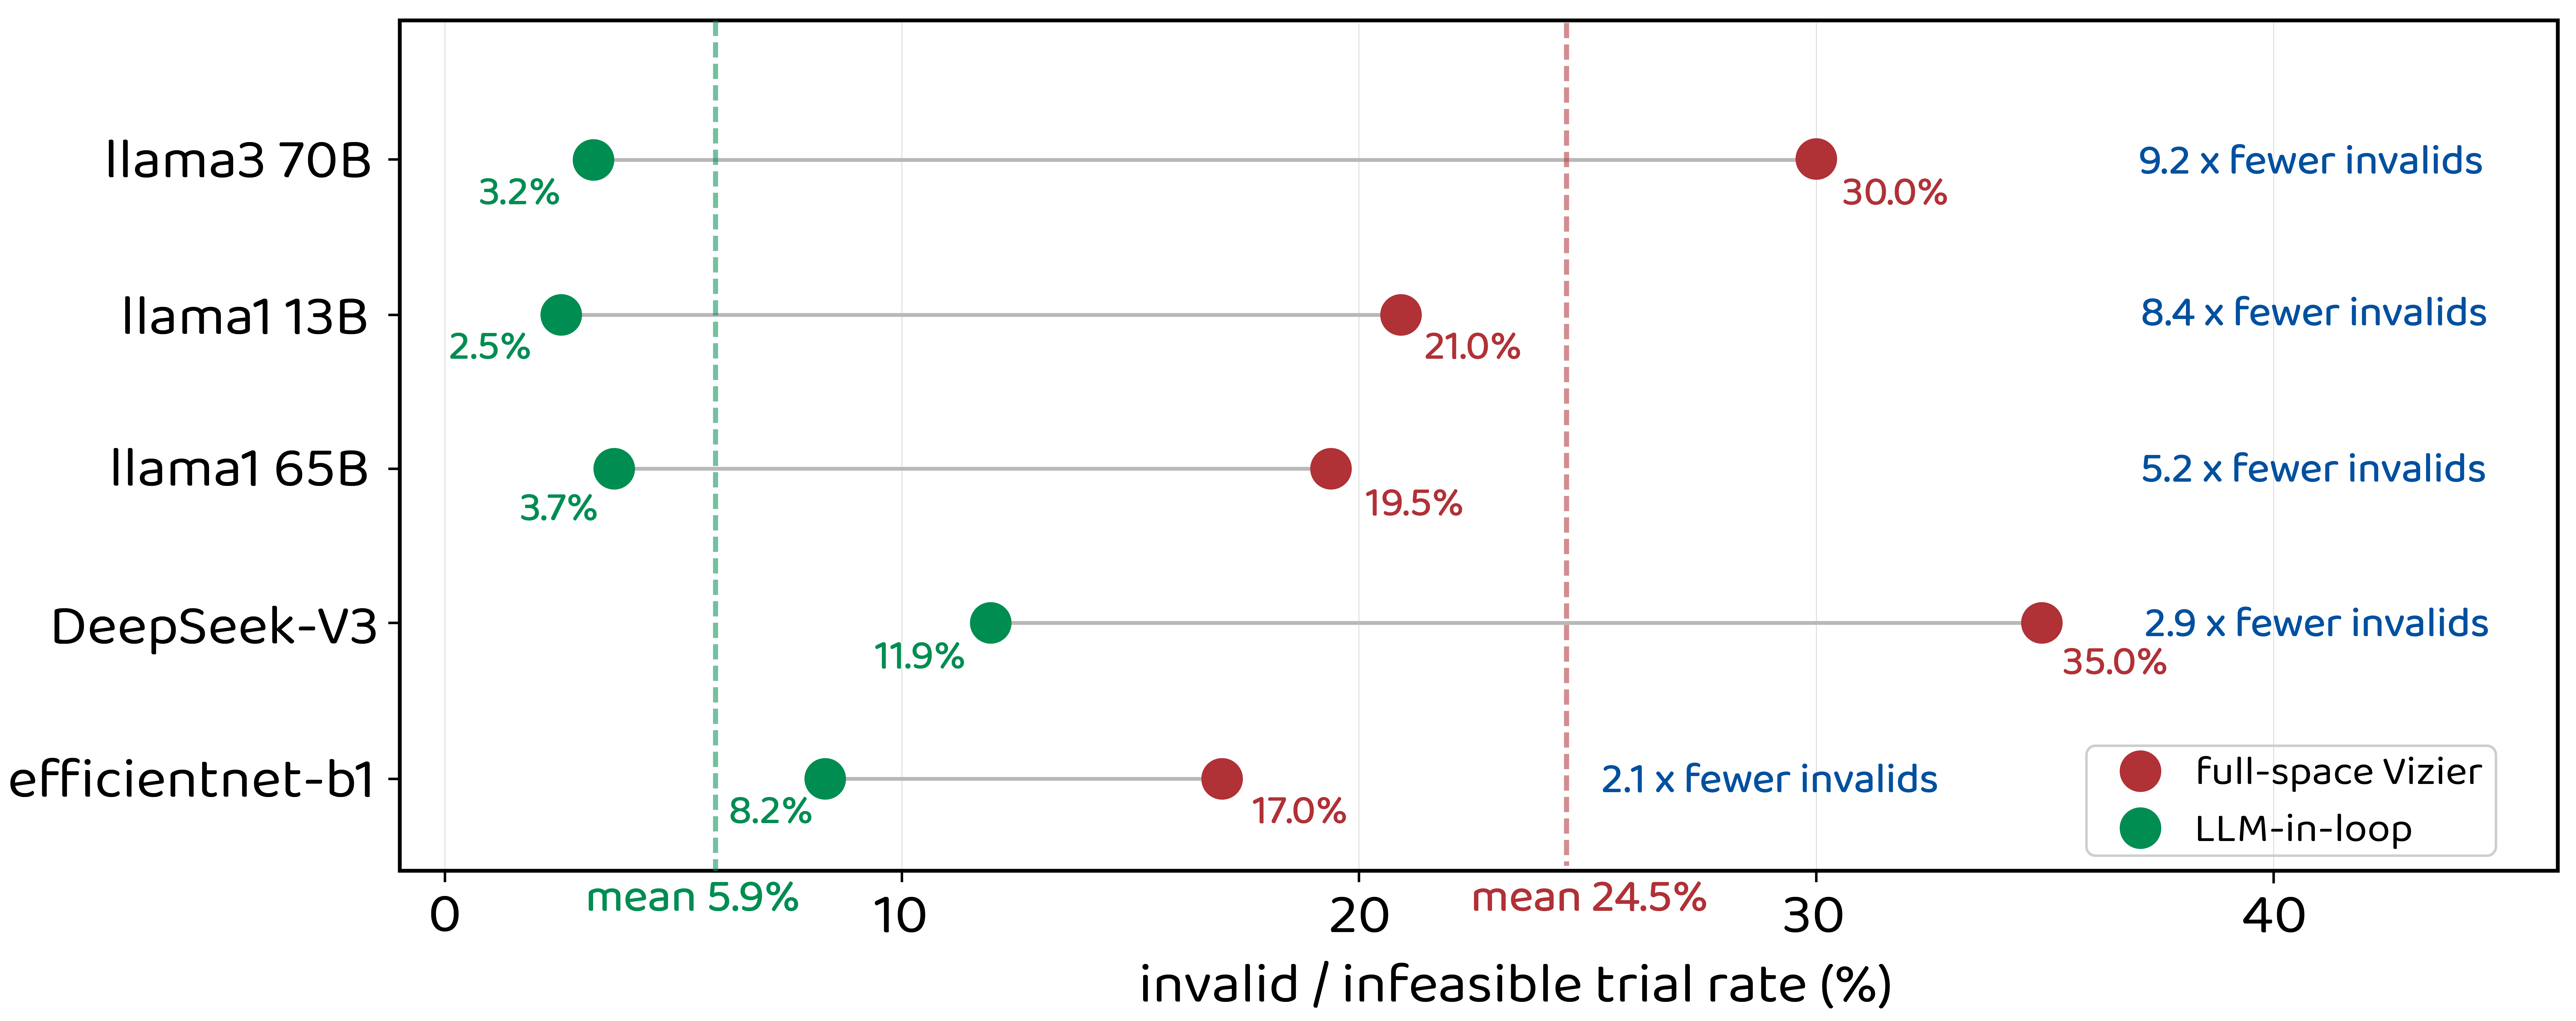
\includegraphics[width=0.85\linewidth]{fig3/llm_guide_v1.png}
% \caption{Strategic Intelligence vs. Stochastic Brute Force}\label{fig:llm}
% \end{figure}



% % The LLM should not just ask, “What chip has the best Perf/TDP?” We aim to answer the question “Given this user’s workload and deployment goal, what is the architectural region to search for this deployment task?”. Therefore we have the LLM emit profile-conditioned campaigns that take specific user inference tasks into consideration. For each $(\text{deployment profile},\ \text{workload})$ cell, we ran a
% % 200-trial LLM-Architect experiment using the same Qwen2.5-7B-Instruct + LoRA with differing user input profiles. At the start of each round, the prompt was assembled from a fixed system
% % prompt, the active deployment profile, three few-shot examples, and a per-round user message containing the workload, recent feedback signals, current search bounds, and the causal ledger.
% % The Strategist returned a one-line JSON campaign patch, which the
% % validator accepted only if it was a strict legal subset of the parent space, satisfied hard rules such as patch-volume $\leq 10\%$, ridgepoint and MAC/BW constraints, and avoided forbidden regions.

% % Thus, the experiment isolates whether the profile-conditioned LLM prompt alone can steer the same V1 evaluator toward different hardware families under different deployment intents.



% % \todo{Compare convergence rate of LLM-guided hardware search vs.\ Vizier-only (Bayesian, LCS, random baselines) in the style of FAST Figure~11. Report:
% % \begin{itemize}
% %     \item Number of trials to reach $X\%$ of best Perf/TDP found by 5,000-trial Vizier
% %     \item Quality of LLM-proposed configurations vs.\ Vizier-proposed configurations
% %     \item Qualitative analysis of LLM reasoning about hardware bottlenecks
% % \end{itemize}
% % }

% % \subsubsection{ROI Analysis}

% % \todo{Update FAST's ROI analysis (Table~4) with the improved Perf/TDP numbers from FAST-CORGI. Report deployment volumes required to reach 1$\times$, 2$\times$, 4$\times$ ROI targets. If Perf/TDP improvements are larger than FAST's, the break-even deployment volume should decrease correspondingly.}

% % \subsubsection{Pareto Frontier}

% % \todo{Plot the Perf/TDP vs.\ area Pareto frontier for V1-optimized designs compared to FAST and TPU-v3 baseline, analogous to FAST Figure~12.}


% edit for page limit
% \vspace{-0.3cm}
\section{Experiments}
\label{sec:experiments}
Experiments span full CHEETAH V0 and V1 pipelines and the LLM Architect across $12$ workloads: $11$ vision and language models plus the Stable Diffusion~1.5 UNet. We benchmark against TPU-v3 because it is the production deep learning accelerator with the most publicly documented microarchitecture, process, and power figures~\citep{jouppi2017datacenter,jouppi2021ten}, which lets every comparison be normalized to a disclosed chip and stay consistent with prior work~\citep{zhang_fast}. For the fixed-hardware study we add a second, deliberately generic hardware point, a compact edge NPU (Section~\ref{sec:fixed_hw}), so that the scheduling gains are shown on both ends of the provisioning spectrum.
~\cref{sec:exp_intro} introduces our experimental setting, sanity checks, and physical manufacturability validation gates.
~\cref{sec:prog} examines progressive unlocked speedup gains between LP formulations,~\cref{sec:breakdown} provides the breakdown of accelerator performance,
~\cref{app:custom_solve} summarizes our custom systems solver design, and~\cref{app:blueprint_tables} provides discussion on CHEETAH custom accelerator blueprint analysis.
% \vspace{-0.2cm}




\subsection{Experimental Setup}
\label{sec:exp_intro}
% \vspace{-0.2cm}
We benchmark against the static FAST framework~\citep{zhang_fast} using a simulated TPU-v3 \citep{jouppi2021ten} baseline normalized to sub-10nm process technology (within $8.2 \pm 2.7\%$ of profiled TPU-v3 performance). We use a custom adapted JAX PDLP solver for large models (Llama-70B, DeepSeek-V3) and HiGHS \citep{huangfu2018parallel} for smaller models, reporting speedup over the TPU-v3 baseline in order to be consistent with prior work.
We evaluate across 12 workloads: EfficientNet-B1 \citep{tan2019efficientnet} through B7 (stressing low-intensity depthwise convolutions), Llama-1 13B/65B and Llama-3 70B \citep{llama3modelcard}, DeepSeek-V3-MoE \citep{deepseekv3report} (stressing memory capacity and bandwidth), and the Stable Diffusion~1.5 UNet, a $346$-operation diffusion backbone with long skip connections (stressing bandwidth-bound activation traffic). Each workload is optimized independently under 100 trials per method. For Static and V0 methods, the pipeline is Vizier$\to$Timeloop$\to$LP; for the V1 method, the pipeline simplifies to Vizier$\to$LP. 
The LLM Architect outer loop proposes search-space interventions for Vizier using Lagrangian dual feedback, and is only permitted to change Vizier's search neighborhood while the strict LP inner loop remains unchanged.

\paragraph{Physical Design Validation.} Since modeling simulations ultimately present a gap with real world physical performance, we validate all results through a five-level audit process: (i) Roofline Auditor, (ii) Campaign Validator, (iii) Causal Ledger, (iv) solver diagnostics, and (v) six pre-RTL gates. Each CHEETAH design must pass all five audit tiers before it is deemed feasible and reported. 

The roofline auditor confirms the basic and necessary condition that the reported LP latency is not physically impossible: no result is faster than either the compute or memory lower bound. All reported CHEETAH results are roofline-feasible with zero lower-bound violations. 
The pre-RTL manufacturability gates aim to ensure that CHEETAH-designed chips can fit a single TSMC N7 reticle, has a wirable pin-out for four HBM3 stacks, meets $1\,\mathrm{GHz}$ timing, has a wirable NoC, fits an AIO cooler envelope, and decomposes into standard SRAM macros.
This seeks to close the gap between simulation at research-level, and a physical design chip that could plausibly be taped out.
\cref{tab:mfg_gates} summarizes the six gate definitions, with detailed numerical reports and discussion provided in Appendix~\ref{app:details}. 


\begin{table}[t]
\centering
\small
\caption{Manufacturability gate definitions. Each candidate hardware configuration must pass all six gates before being accepted as a feasible design, rather than a theoretical Pareto-frontier point that exists only in LP space. These are not post-hoc screens applied to a finished design: every one of them is a row of the program itself, so the optimizer cannot return a design that violates them. The pin-count limit, for instance, enters as a linear constraint on bandwidth, which removes the illegal bandwidth branches from the menu before any design is scored. A gate can therefore only be reported as satisfied, never as repaired.}
\label{tab:mfg_gates}
\begin{tabularx}{\linewidth}{lXr}
\toprule
\textbf{Gate} & \textbf{What it checks} & \textbf{Threshold} \\
\midrule
1.\ Pin count    &
  HBM3-class signal pins at $0.8$\,GB/s/pin &
  $\le 4{,}096$ pins \\[0.3em]
2.\ Reticle area &
  Linear area model on 7\,nm &
  $\le 600$\,mm$^2$ \\[0.3em]
3.\ Logic depth  &
  MAC-tree combinational depth &
  $\le 35$ levels \\[0.3em]
4.\ NoC routing  &
  $n_{\mathrm{PEs}} \times n_{\mathrm{banks}}$ cells &
  $\le 5\times10^6$ \\[0.3em]
5.\ Power density &
  $P_{\mathrm{dyn}} / A_{\mathrm{die}}$ &
  $\le 2.0$\,W/mm$^2$ \\[0.3em]
6.\ SRAM macros  &
  64\,KiB banks; aspect ratio $\in [1{:}4,\, 4{:}1]$ &
  $\le 4{,}096$ banks \\
\bottomrule
\end{tabularx}
\end{table}



% \subsection{Main Results}

% \subsubsection{V0 vs.\ FAST Static Fusion}

% \todo{Insert results table and figure comparing V0 (time-indexed placement + rematerialization) against FAST's static fusion ILP on all benchmarks. Key metrics: Perf/TDP improvement, fusion efficiency (\% of DRAM stall time eliminated), rematerialization frequency (how often does the solver choose to recompute rather than reload?).}

% \paragraph{Expected findings.}
% V0's dynamic placement should show the largest gains on workloads with: (1)~tight Global Memory budgets where static pinning wastes capacity on tensors that are only needed briefly, (2)~long dependency chains where tensor lifetimes vary substantially, and (3)~cheap-to-recompute operations with large activations (\eg, depthwise convolutions in EfficientNet).

% \subsubsection{V1 vs.\ V0: Joint Tiling and Fusion}

% \todo{Insert results table and figure comparing V1 against V0 on all benchmarks. Key metrics: Perf/TDP improvement, number of operations where V1 selects a different tiling configuration than Timeloop's greedy choice, and the resulting compute efficiency vs.\ fusion trade-off.}

% \paragraph{Expected findings.}
% V1 should show the largest gains on architectures with highly diverse layer types where a single tiling configuration cannot serve all operations well. EfficientNet (depthwise + pointwise convolutions with 100$\times$ variation in working-set sizes) and hybrid CNN-transformer models (convolutions + attention + MLP with fundamentally different compute-memory profiles) are expected to benefit most.


% \subsubsection{stiatic vs v0 vs v1}
% \begin{figure}[ht!]
%     \centering
%     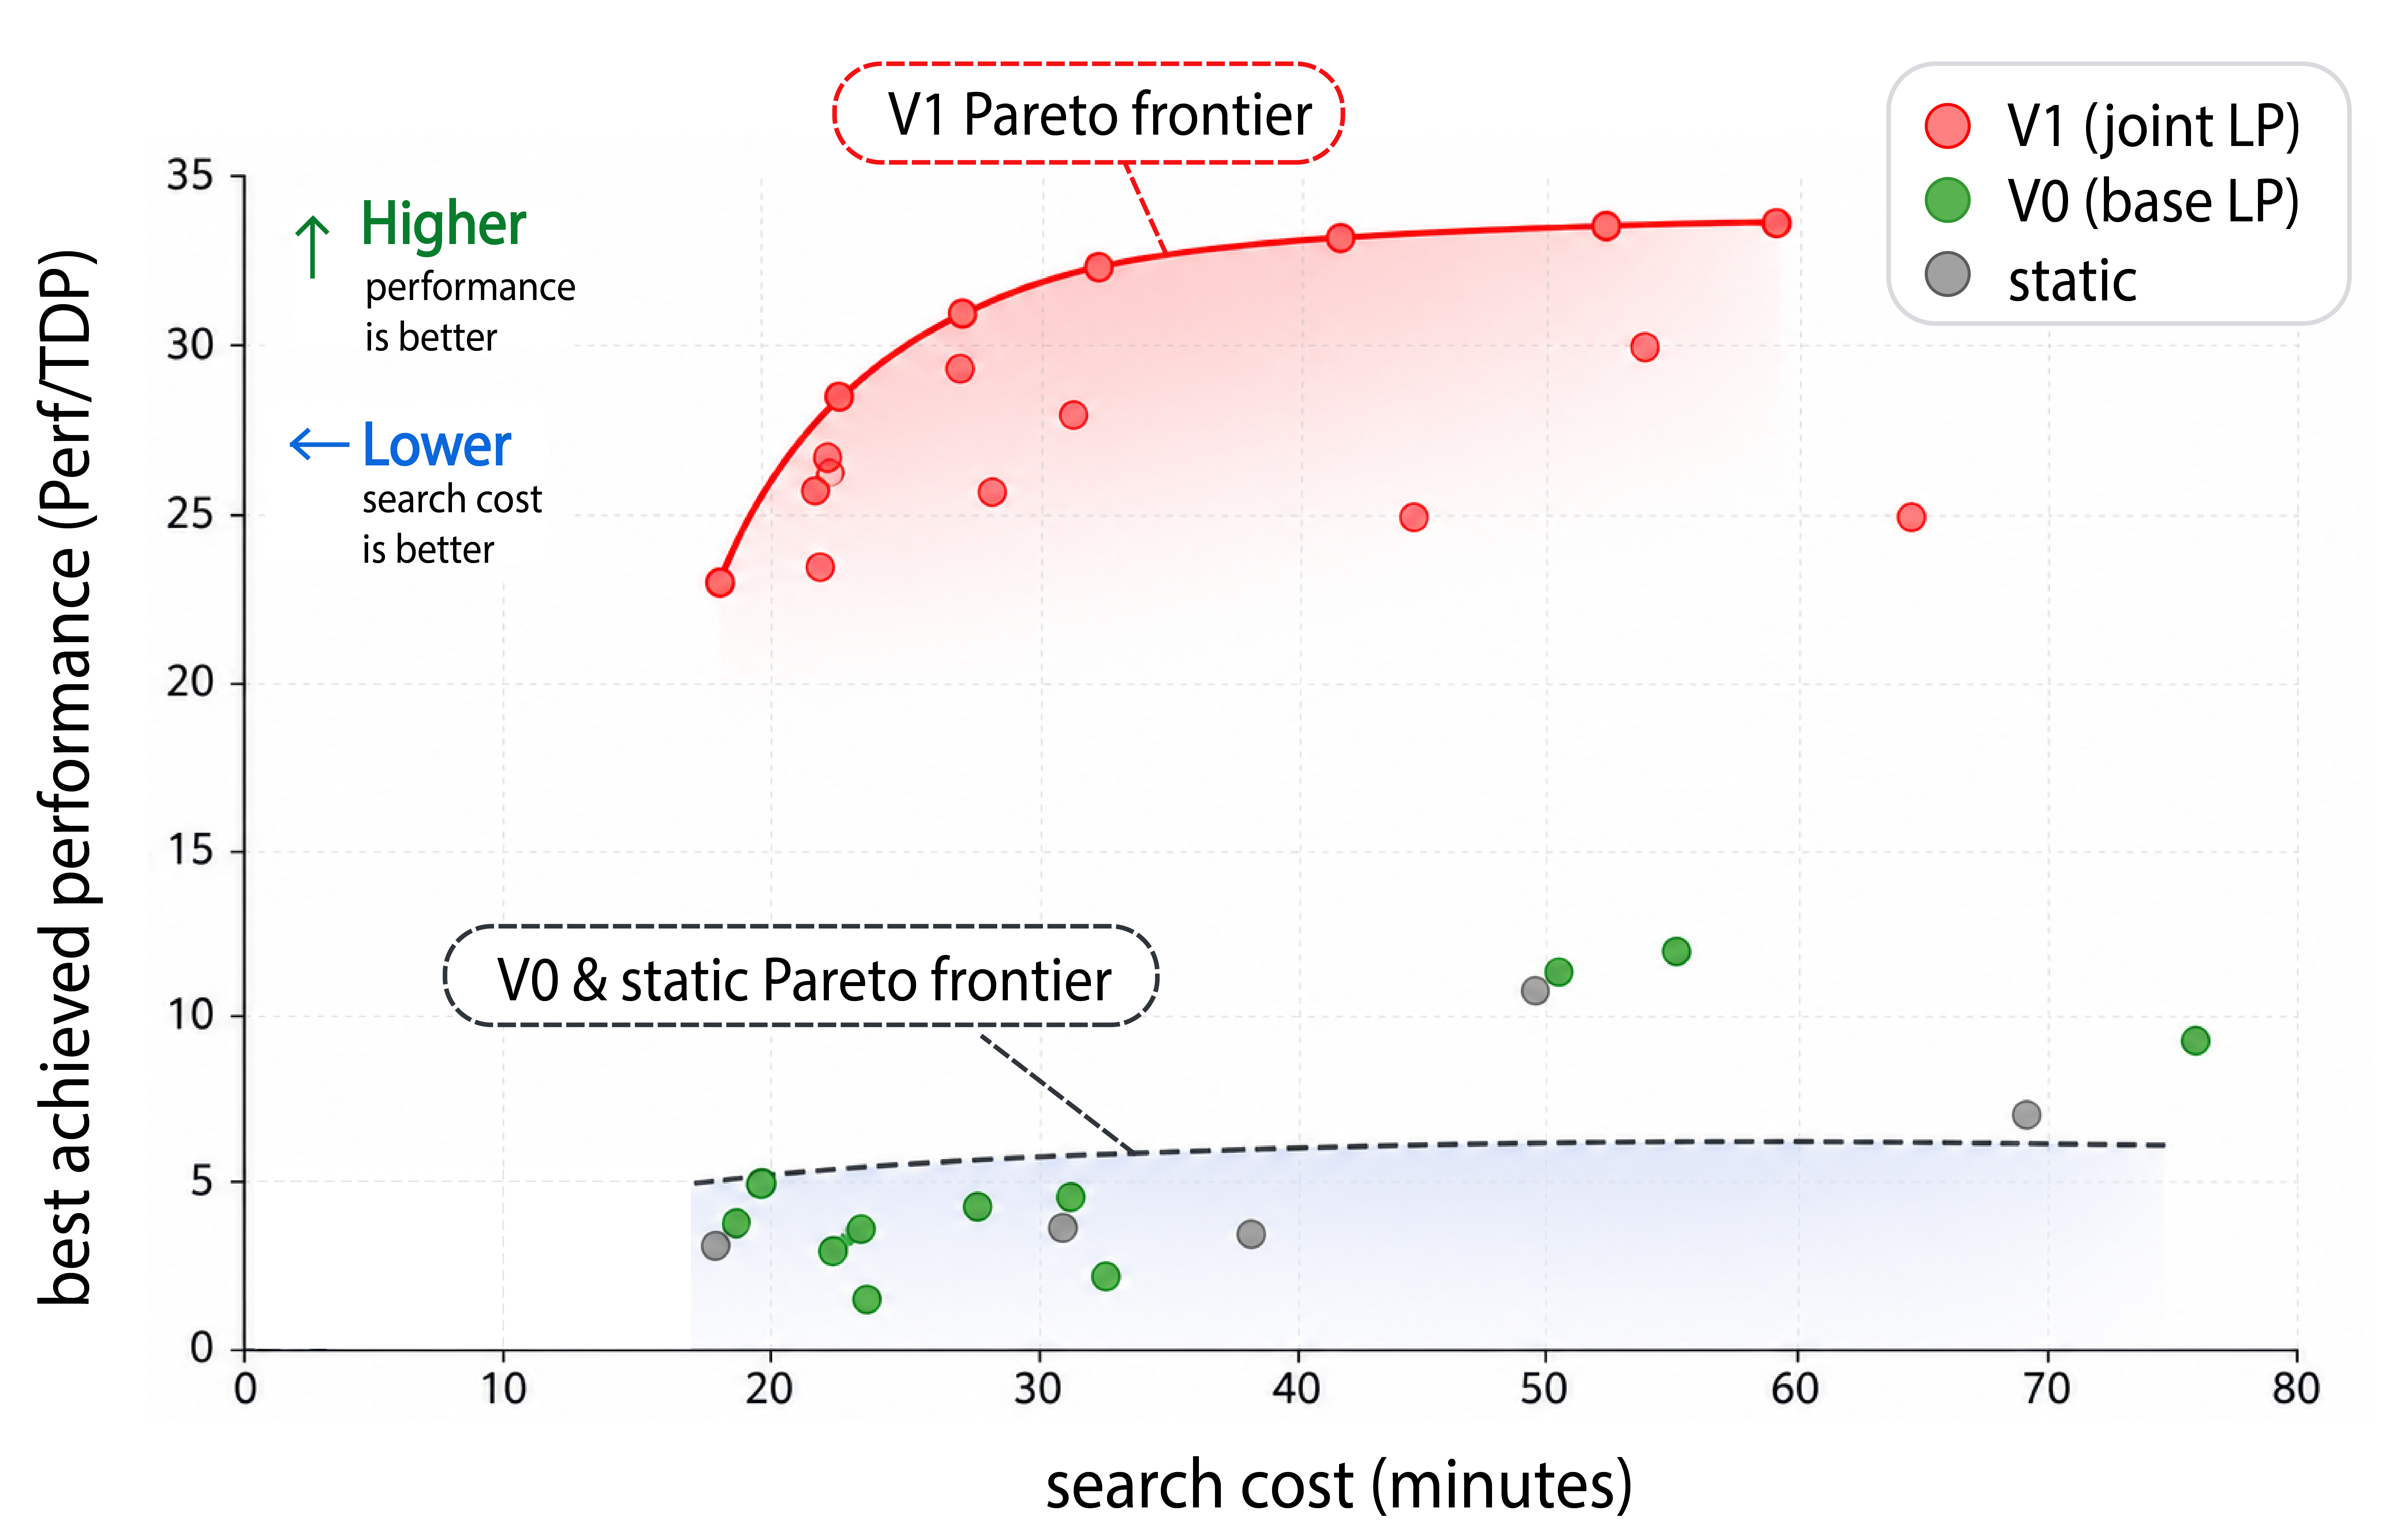
\includegraphics[width=0.7\linewidth]{figs/pareto_v2.png}
%     \caption{pareto frontier plot}
% \end{figure}
\begin{figure}[ht!]
    \centering
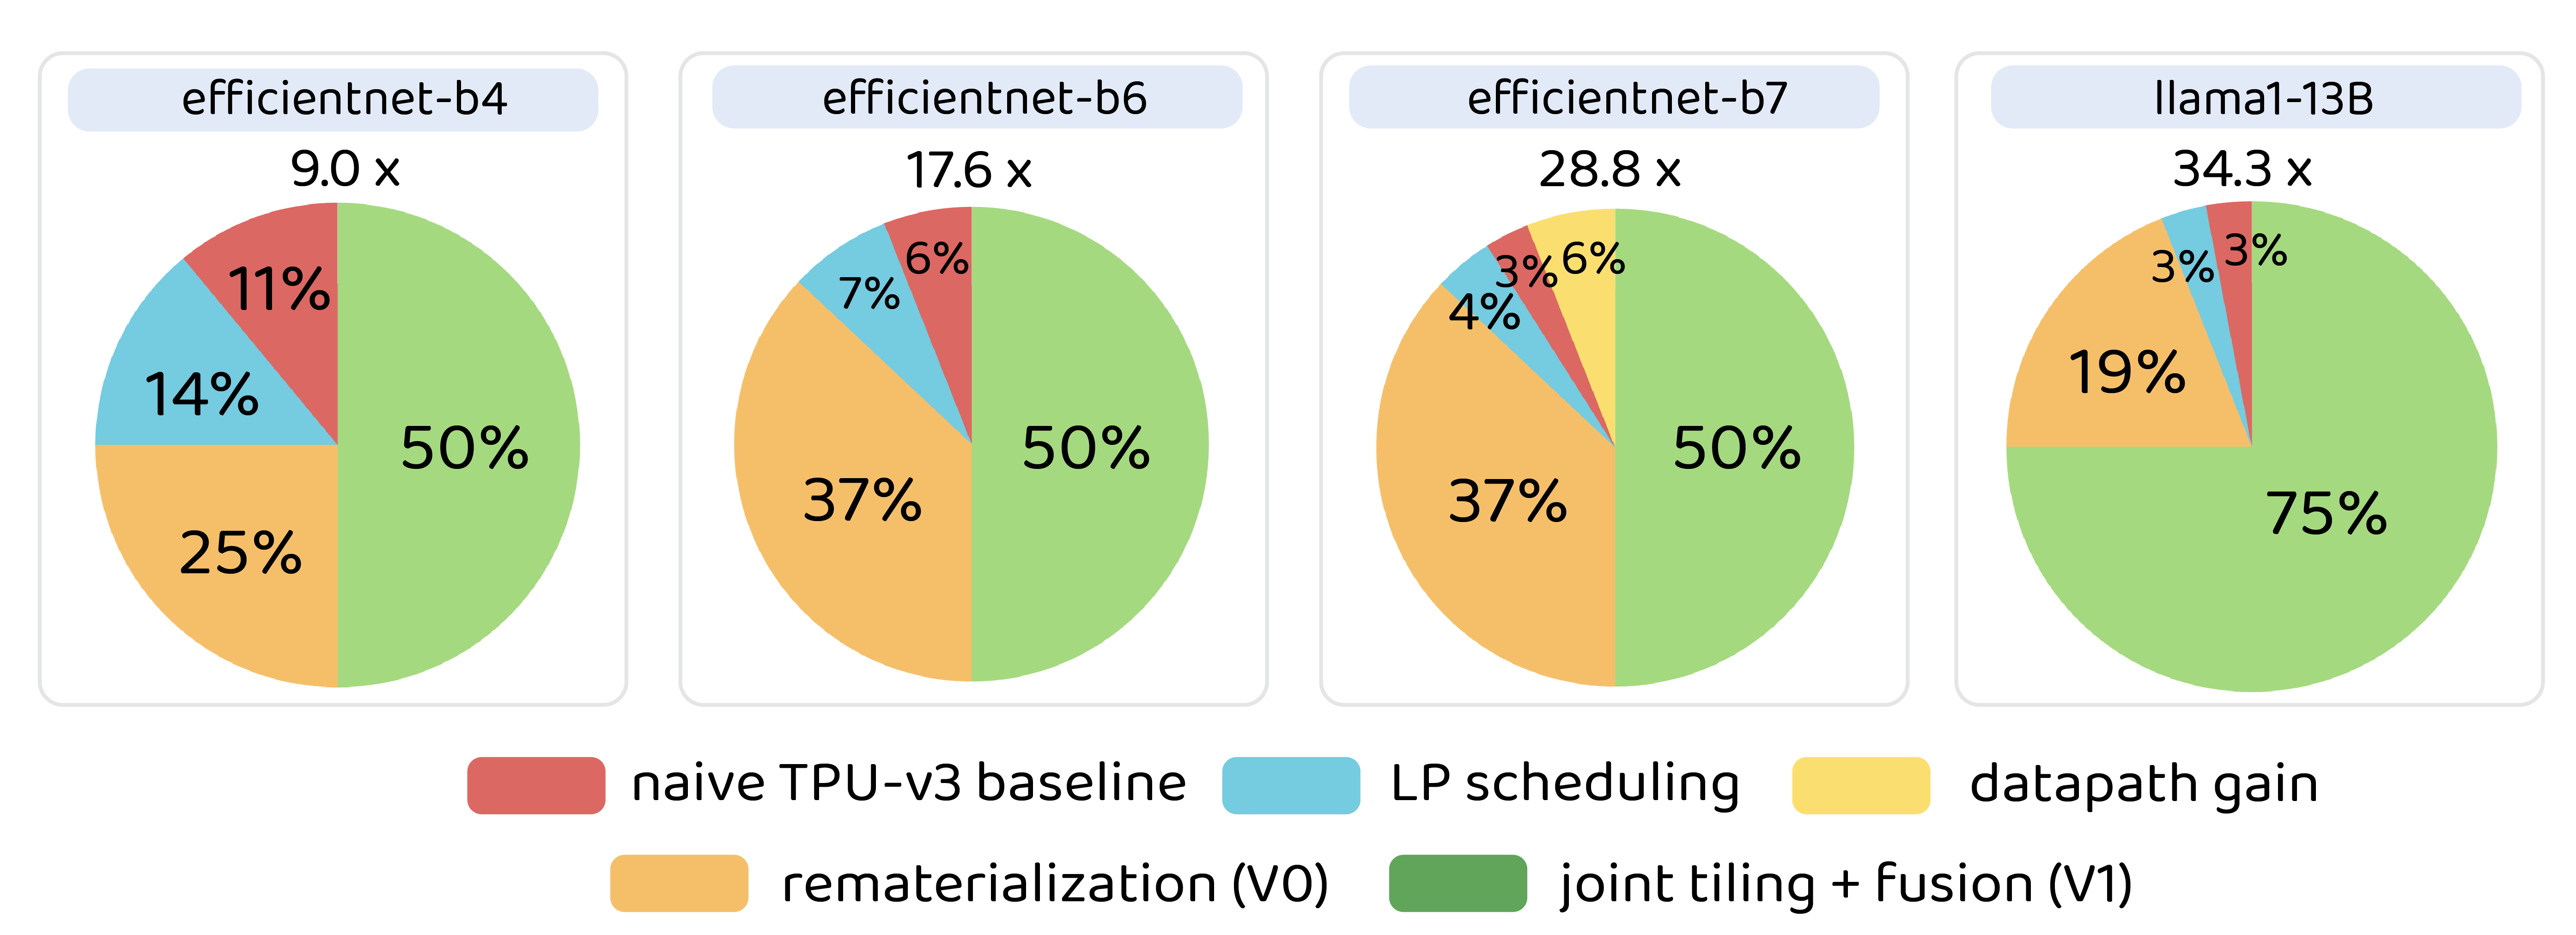
\includegraphics[width=0.85\linewidth]{fig3/speedup_decomposition_final_v4.png}
\caption{Speedup decomposition over naive TPU-v3 baseline. Each pie shows the 
relative contribution of four optimization sources to the total speedup. CHEETAH-V1 joint tiling + fusion dominates on all workloads, 
especially on larger models where memory management is the primary bottleneck.}\label{fig:accel_decompose}
\end{figure}
\subsection{Static Baseline vs.\ CHEETAH-V0 vs.\ CHEETAH-V1 Unlock Progressive Gains}
\label{sec:prog}

Figure~\ref{fig:accel_decompose} decomposes the total speedup over a naive TPU-v3 baseline into four sources: LP-based scheduling and fusion, datapath gain from hardware search, dynamic rematerialization (CHEETAH-V0), and joint tiling + fusion (CHEETAH-V1). Table~\ref{tab:LP_struct} in \cref{append::lp_perform} gives side-by-side structural comparison of the V0 and V1 formulation matrices in greater detail. 

The dominant contributor across all workloads is V1's joint tiling-fusion 
optimization. V1's share grows with model size: from 50\% on B1--B4 to 75--88\% from B5 onward and 83--87\% on Llama, reflecting that memory management increasingly dominates as models scale. On smaller models, LP scheduling and datapath gains split the remainder; V0 rematerialization contributes ${\sim}25\%$ on B3--B4 where recomputing large depthwise activations outperforms DRAM reloads.

Critically, Figure~\ref{fig:speedup} shows the static fusion method is \emph{infeasible} on modern large models (Llama-70B, and DeepSeek-V3), because their large activation tensors cannot fit under a static pinning policy. The V0 formulation resolves feasibility on large models via dynamic placement, while V1 further improves by jointly selecting memory-efficient tiling configurations alongside placement, achieving feasibility across the entire workload suite. This demonstrates that joint optimization is not merely an incremental improvement but a qualitative capability unlock for large-scale models. Additional optimization details and observations are provided in Appendix~\ref{app:details}. We further provide two interesting examples of optimal tiling solutions the V1 formulation proposed in Appendix~\ref{app:tiling}.

\begin{figure}[ht!] 
    \centering
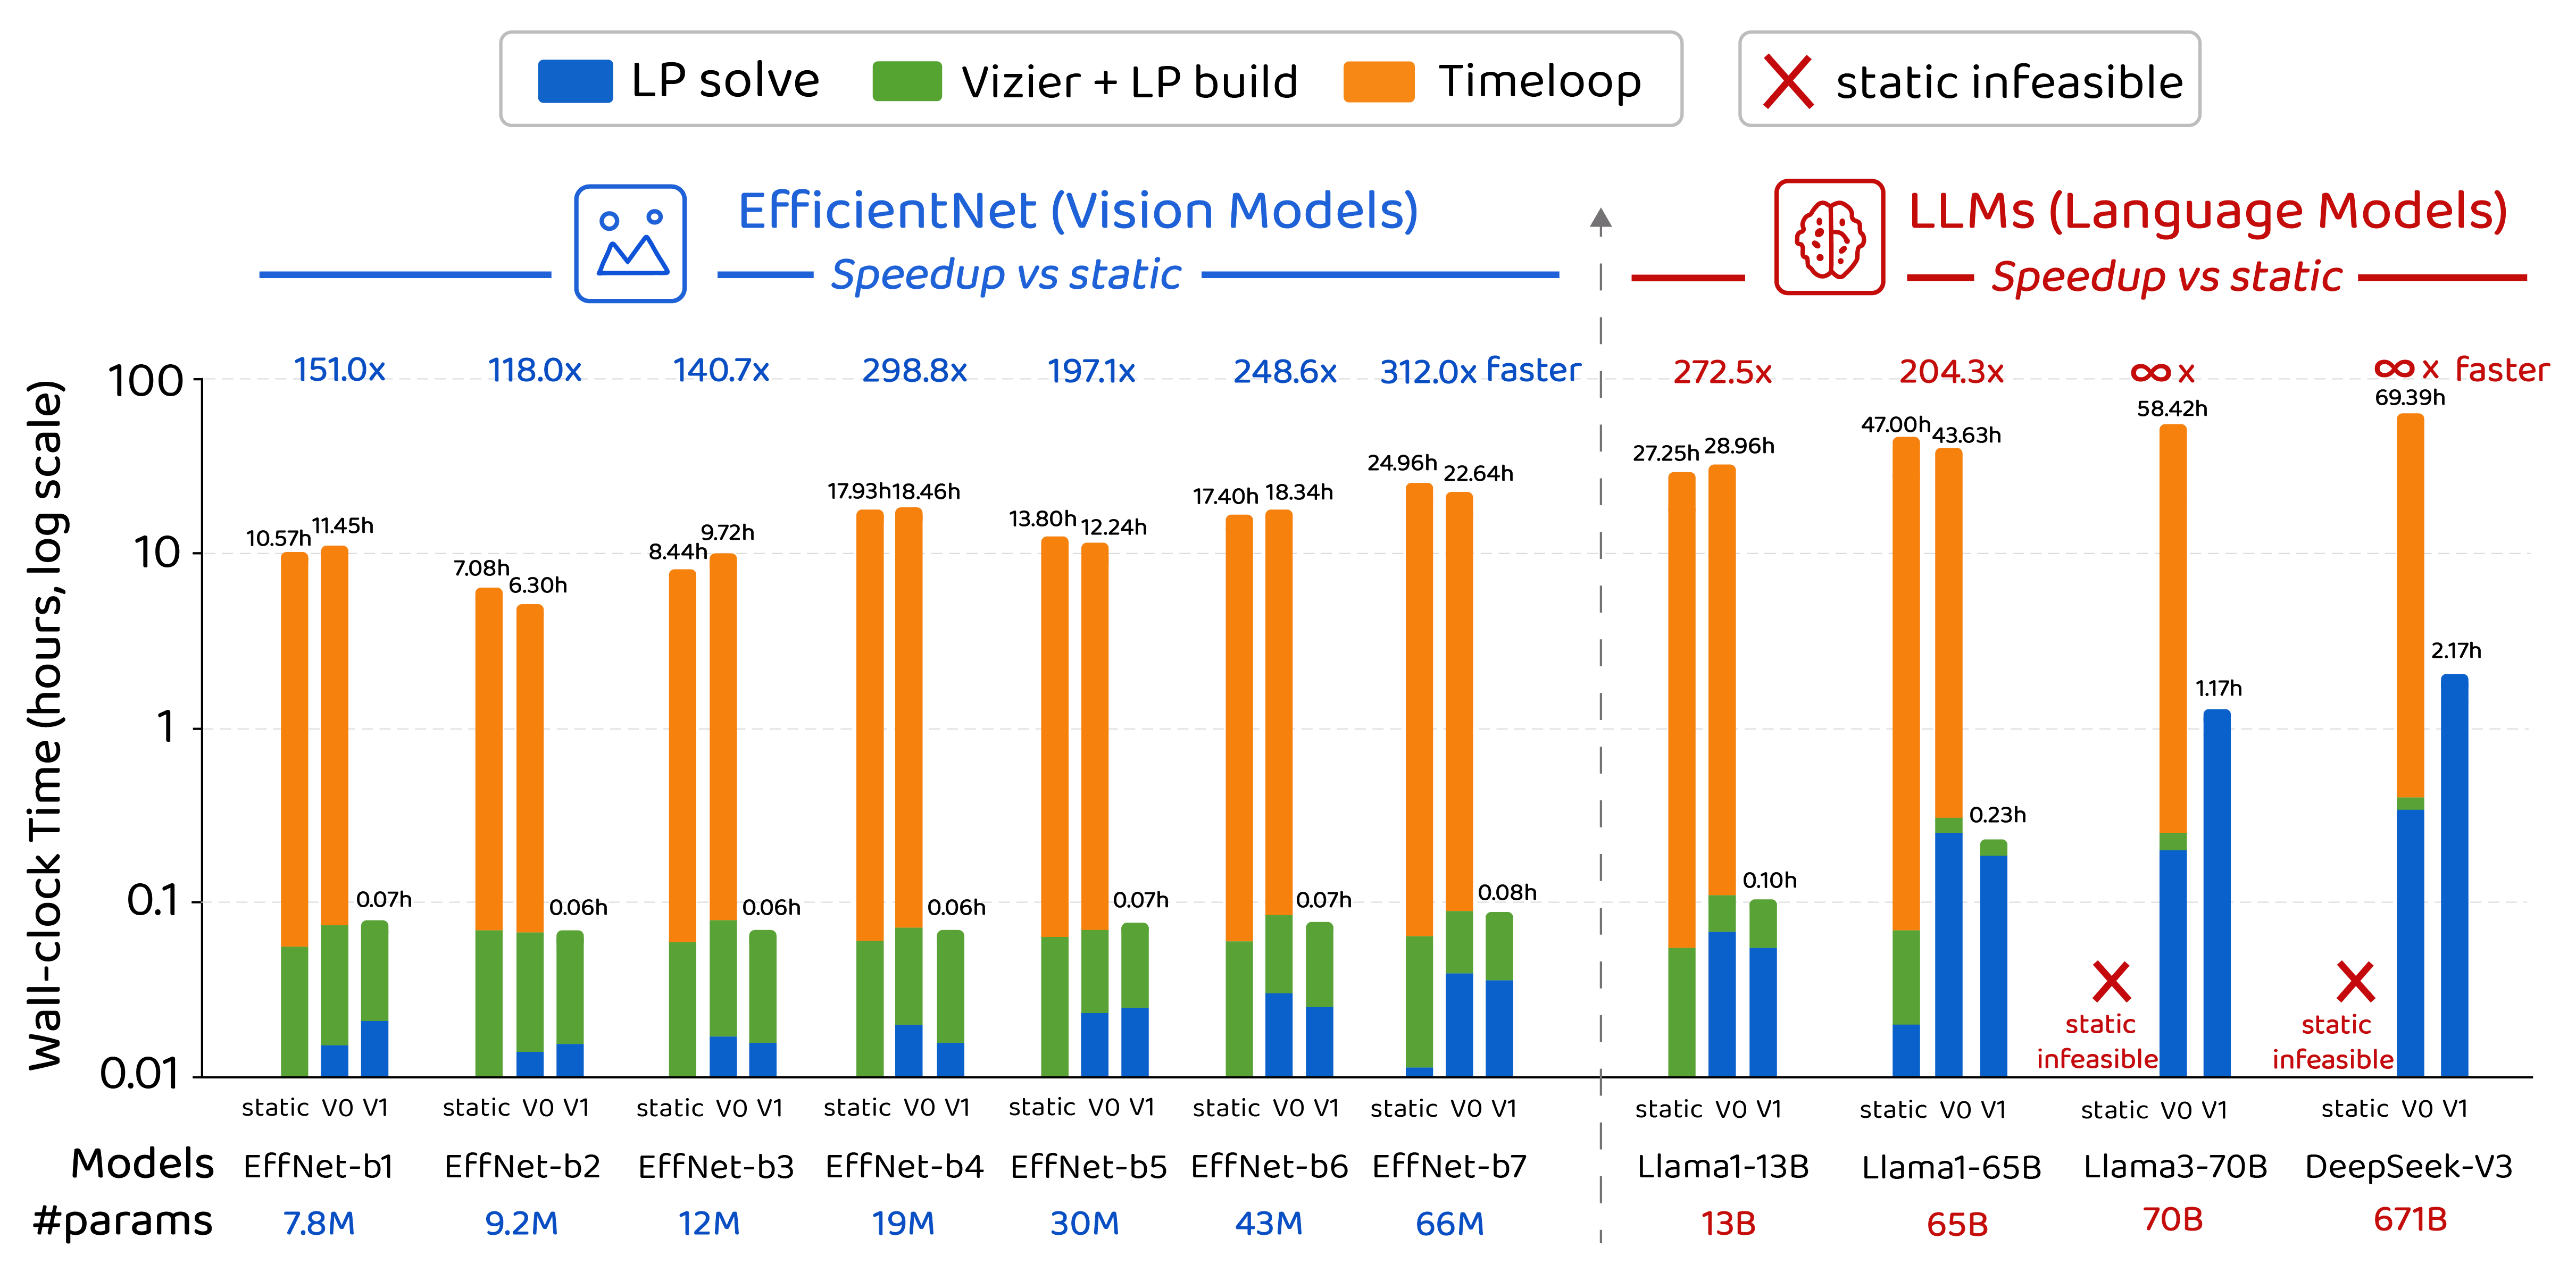
\includegraphics[width=1.0\linewidth]{fig3/wallclock_new_v6.png}
\caption{Wall-clock time decomposition and performance acceleration across formulations: CHEETAH-V1's internalized tiling eliminates the Timeloop bottleneck, achieving up to 100--300$\times$ faster search than the classical static method. Upper bars show wall-clock hours (log scale); annotations show speedup vs.\ static.}
\label{fig:wallclock}
\end{figure}

\subsection{Same-Silicon Fixed-Hardware Speedup}
\label{sec:fixed_hw}
The speedup decomposition of Figure~\ref{fig:accel_decompose} folds hardware search into the reported gains. To isolate CHEETAH's scheduling contribution from silicon provisioning, we hold the chip \emph{fixed} and compare the joint CHEETAH-V1 schedule against a naive streaming schedule on the \emph{same} silicon. Because the identical chip appears in both the numerator and the denominator of every ratio, these speedups are equal-area and equal-TDP by construction and require no resource normalization. We evaluate two fixed-hardware baselines: the simulated TPU-v3 (900\,GB/s, 32\,MiB on-chip) and a compact edge NPU representative of Jetson-Orin-Nano-class parts ($32{,}768$ INT8 MACs at $1$\,GHz, ${\sim}65$\,TOPS, $64$\,GB/s LPDDR5, $16$\,MiB on-chip). We additionally include Stable Diffusion~1.5 UNet (SD1.5-UNet), a $346$-operation diffusion UNet with long skip connections, to stress a bandwidth-bound regime distinct from the CNN and LLM suites.

\begin{table}[t]
\centering
\caption{Same-silicon fixed-hardware speedup: the joint CHEETAH-V1 schedule vs.\ a naive streaming schedule on the \emph{identical} chip. Speedup is $T_{\text{naive}}/T_{\text{joint}}$ under the same cost-model convention on that chip's own per-layer cache (naive $=\sum T_{\max}$ streaming); MFU is model-MFU (cache compute-floor over latency within one convention), not measured silicon utilization. Ratios are equal-area/TDP by construction. Bold marks the best speedup per chip.}
\label{tab:fixed_hw}
\scriptsize
\setlength{\tabcolsep}{4.5pt}
\renewcommand{\arraystretch}{1.22}
\definecolor{bandtpu}{RGB}{230,239,253}
\definecolor{bandnpu}{RGB}{230,245,233}
\definecolor{rowalt}{gray}{0.955}
\definecolor{rowgeo}{gray}{0.875}
\begin{tabular}{@{}l ccc ccc@{}}
\toprule
 & \multicolumn{3}{c}{\cellcolor{bandtpu}\textbf{TPU-v3} (900\,GB/s, 32\,MiB)}
 & \multicolumn{3}{c}{\cellcolor{bandnpu}\textbf{Compact NPU} (64\,GB/s, 16\,MiB)} \\
\cmidrule(lr){2-4}\cmidrule(lr){5-7}
\textbf{Workload} & MFU$_{\text{naive}}$ & MFU$_{\text{joint}}$ & Speedup & MFU$_{\text{naive}}$ & MFU$_{\text{joint}}$ & Speedup \\
\midrule
Llama-1 13B     & 0.467 & 1.000 & $2.14\times$ & 0.022 & 0.694 & $\mathbf{31.4\times}$ \\
\rowcolor{rowalt}
Llama-3 70B     & 0.399 & 1.000 & $\mathbf{2.51\times}$ & 0.043 & 0.330 & $7.66\times$ \\
DeepSeek-V3     & 0.451 & 1.000 & $2.22\times$ & 0.043 & 0.330 & $7.8\times$ \\
\rowcolor{rowalt}
SD1.5-UNet      & 0.643 & 0.963 & $1.50\times$ & 0.038 & 0.223 & $5.89\times$ \\
\midrule
\rowcolor{rowgeo}
\textbf{Geomean} & & & $\mathbf{2.06\times}$ & & & $\mathbf{10.3\times}$ \\
\bottomrule
\end{tabular}
\end{table}

Table~\ref{tab:fixed_hw} reports $T_{\text{naive}}/T_{\text{joint}}$ per cell, where the naive denominator is a $\sum T_{\max}$ streaming schedule computed under the same cost-model convention on each chip's own per-layer cache. On the TPU-v3 the joint schedule delivers $1.50$--$2.51\times$ (geomean $2.06\times$); on the compact NPU the gains are markedly larger, $5.89$--$31.4\times$ (geomean $10.3\times$). This gap is a direct consequence of bandwidth: at $64$\,GB/s the naive streaming schedule is severely memory-starved, running at a model-MFU of only $0.02$--$0.04$, so the placement and residency structure of the joint LP recovers a far larger fraction of idle time. SD1.5-UNet exemplifies this sensitivity: its $1.50\times$ TPU-v3 gain rises to $5.89\times$ on the edge NPU, tracking the same inverse-bandwidth trend as the LLMs because the diffusion UNet is bandwidth-bound once on-chip capacity is tight. All model-MFU values are the cache compute-floor divided by LP latency within a single convention, not measured silicon utilization: on the TPU-v3 the joint schedule recovers model-MFU from a naive $0.40$--$0.64$ to $0.96$--$1.00$ (a near-pure utilization recovery, not additional compute), while on the bandwidth-starved edge NPU the joint model-MFU ($0.22$--$0.69$) is the physical roofline, honestly below one.

\subsection{Wall-Clock Acceleration and LLM Outer Loop Search Efficiency}
\label{sec:breakdown}
Figure~\ref{fig:wallclock} reveals a striking practical advantage of V1: by internalizing tiling into the LP, it removes Timeloop from the per-trial critical path, collapsing each trial to a single Vizier-proposal and LP-solve step. On EfficientNet models, V1 completes 50 trials 151--312$\times$ faster than the static pipeline. On LLMs the acceleration is even more dramatic: V0 requires 58.42 hours on Llama-70B and 69.39 hours on DeepSeek-V3 for 50 trials, whereas V1 requires only 1.17 hours and 2.17 hours respectively, a ${\sim}93\%$ average reduction. This speedup arises because Timeloop accounts for over 99\% of per-trial latency in the sequential pipeline (Figure~\ref{fig:timeloop-time}), and V1 eliminates this bottleneck entirely via precomputed Pareto tiling sets that are reused across all Vizier trials sharing the same compute configuration class. The combination of higher speedup \emph{and} dramatically lower search cost makes V1 strictly dominant: it explores a larger feasible design space in a fraction of the wall-clock time. 

% \begin{wrapfigure}{r}{0.48\textwidth}
% \vspace{-12pt}
% \centering
% 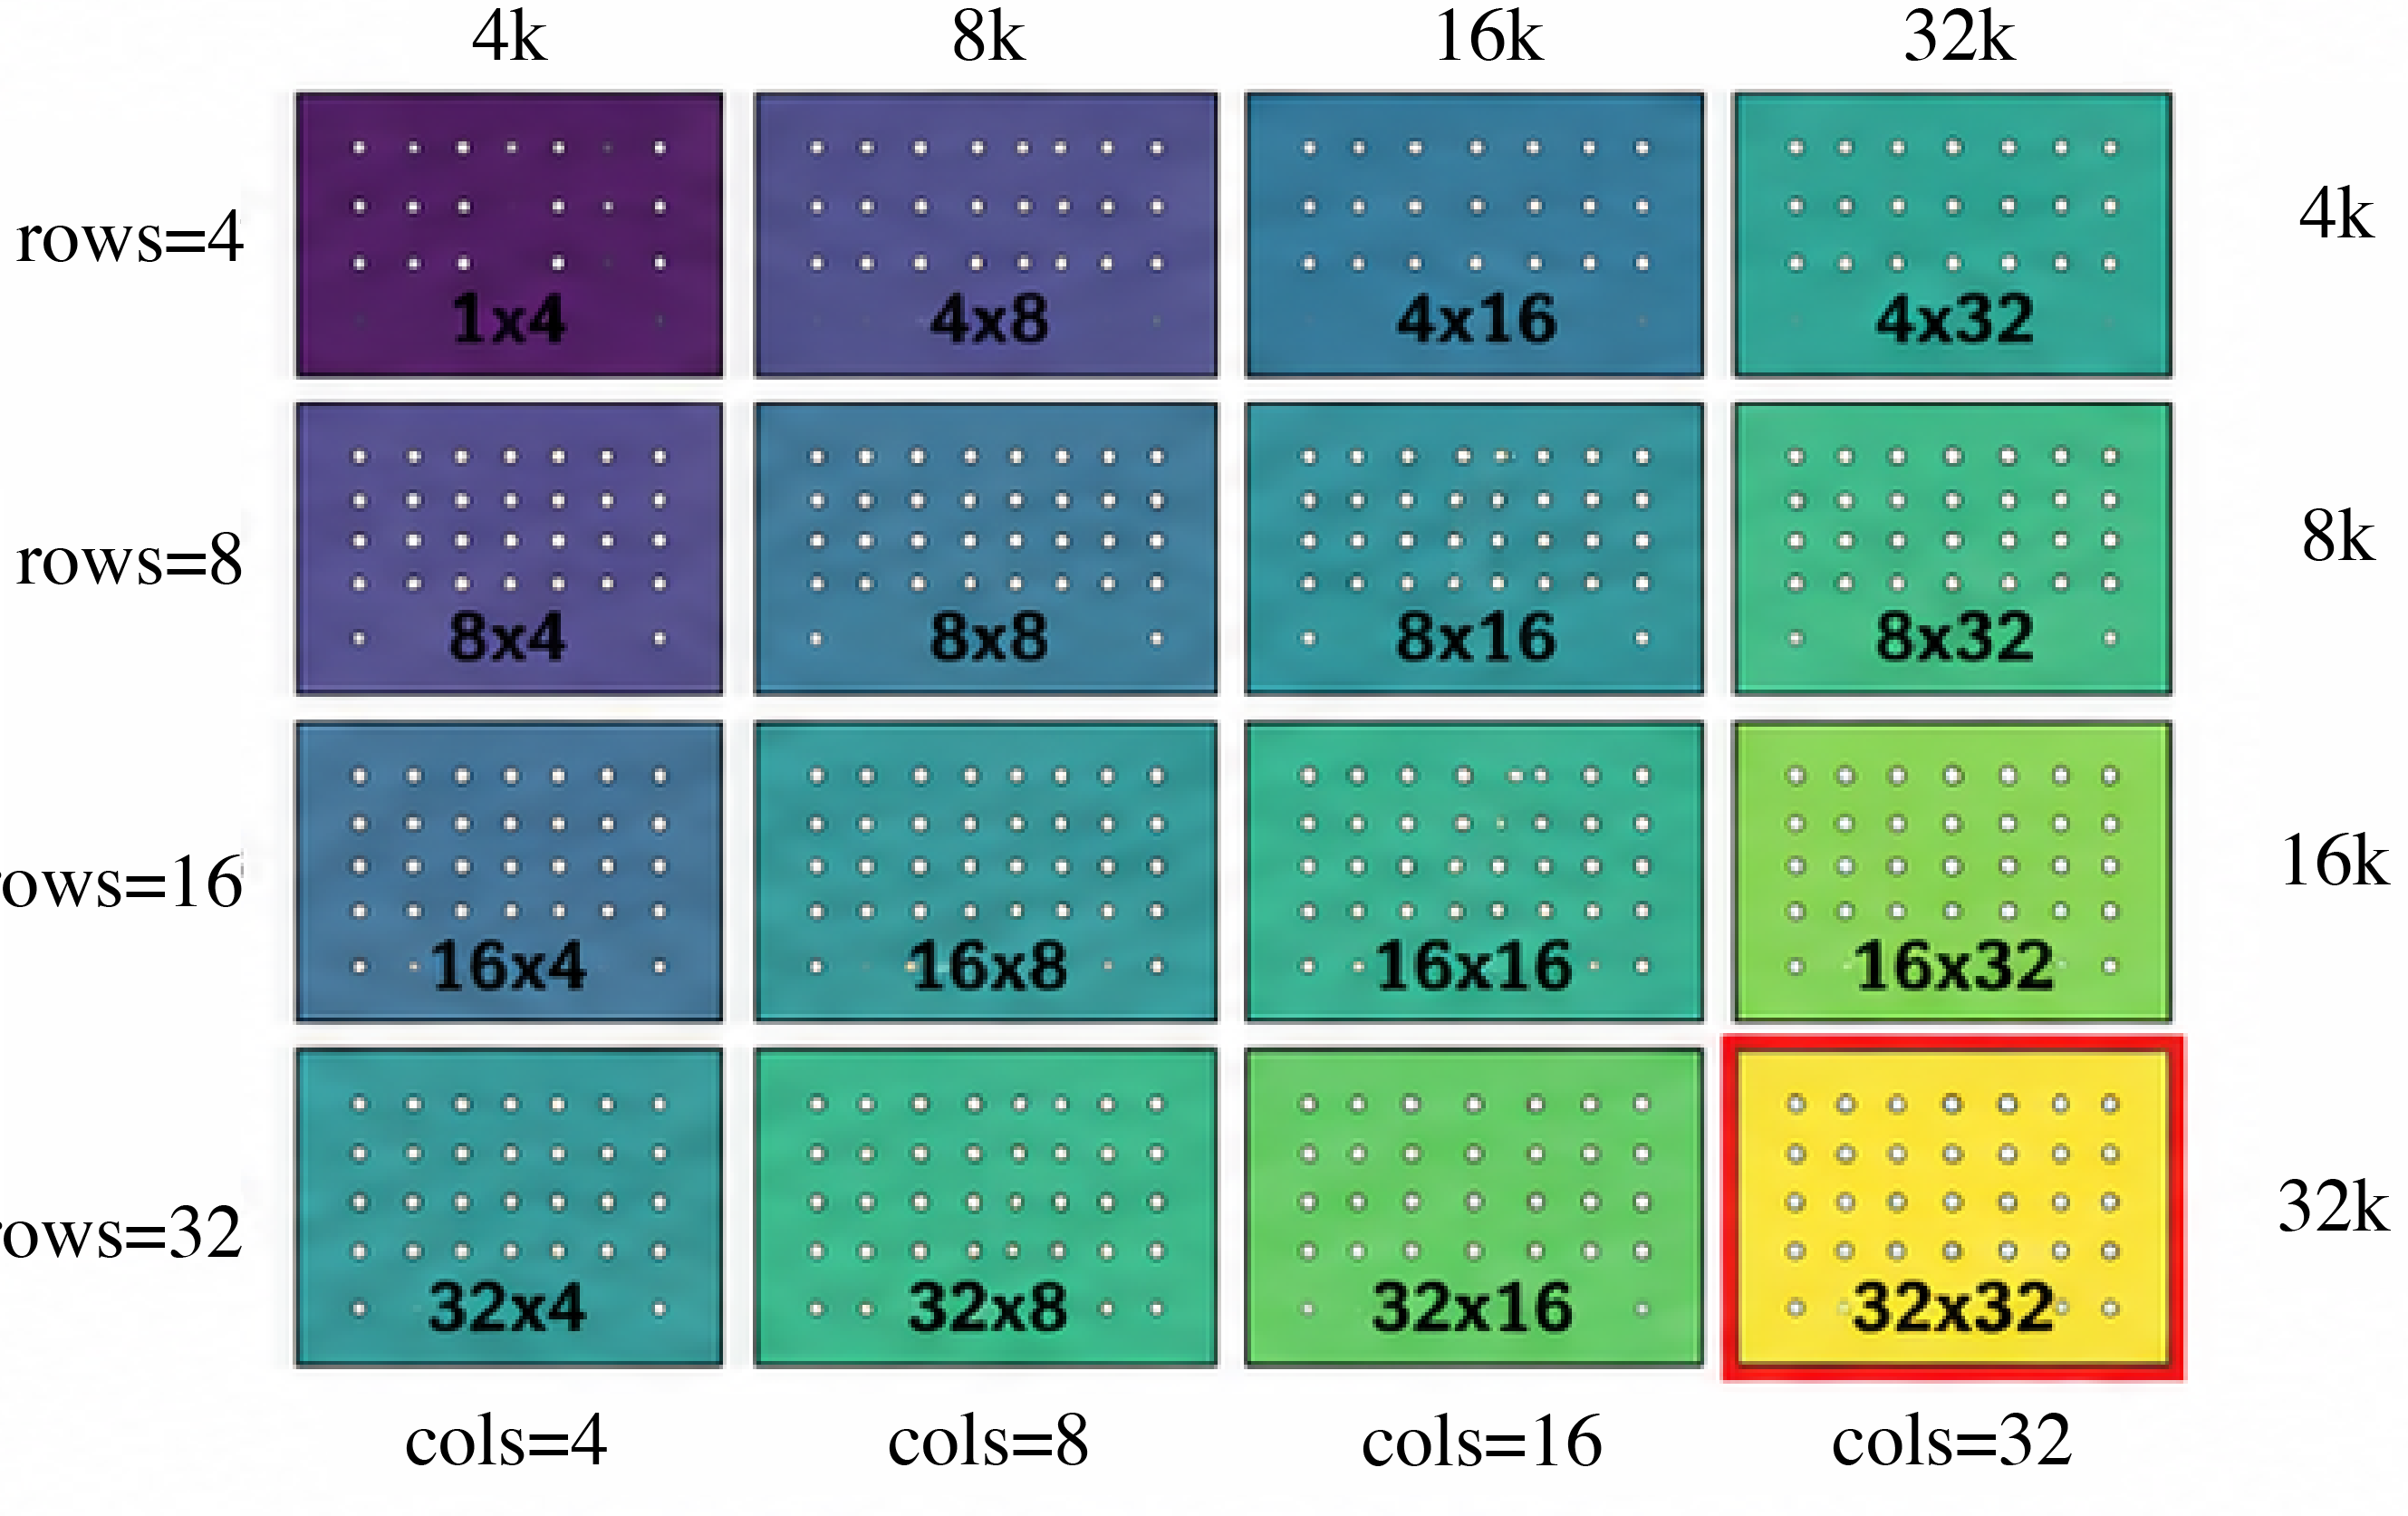
\includegraphics[width=0.46\textwidth]{figs4/tiles.png}
% \caption{Caption here.}
% \label{fig:tiles}
% \vspace{-14pt}
% \end{wrapfigure}
\begin{figure}[h]
\centering
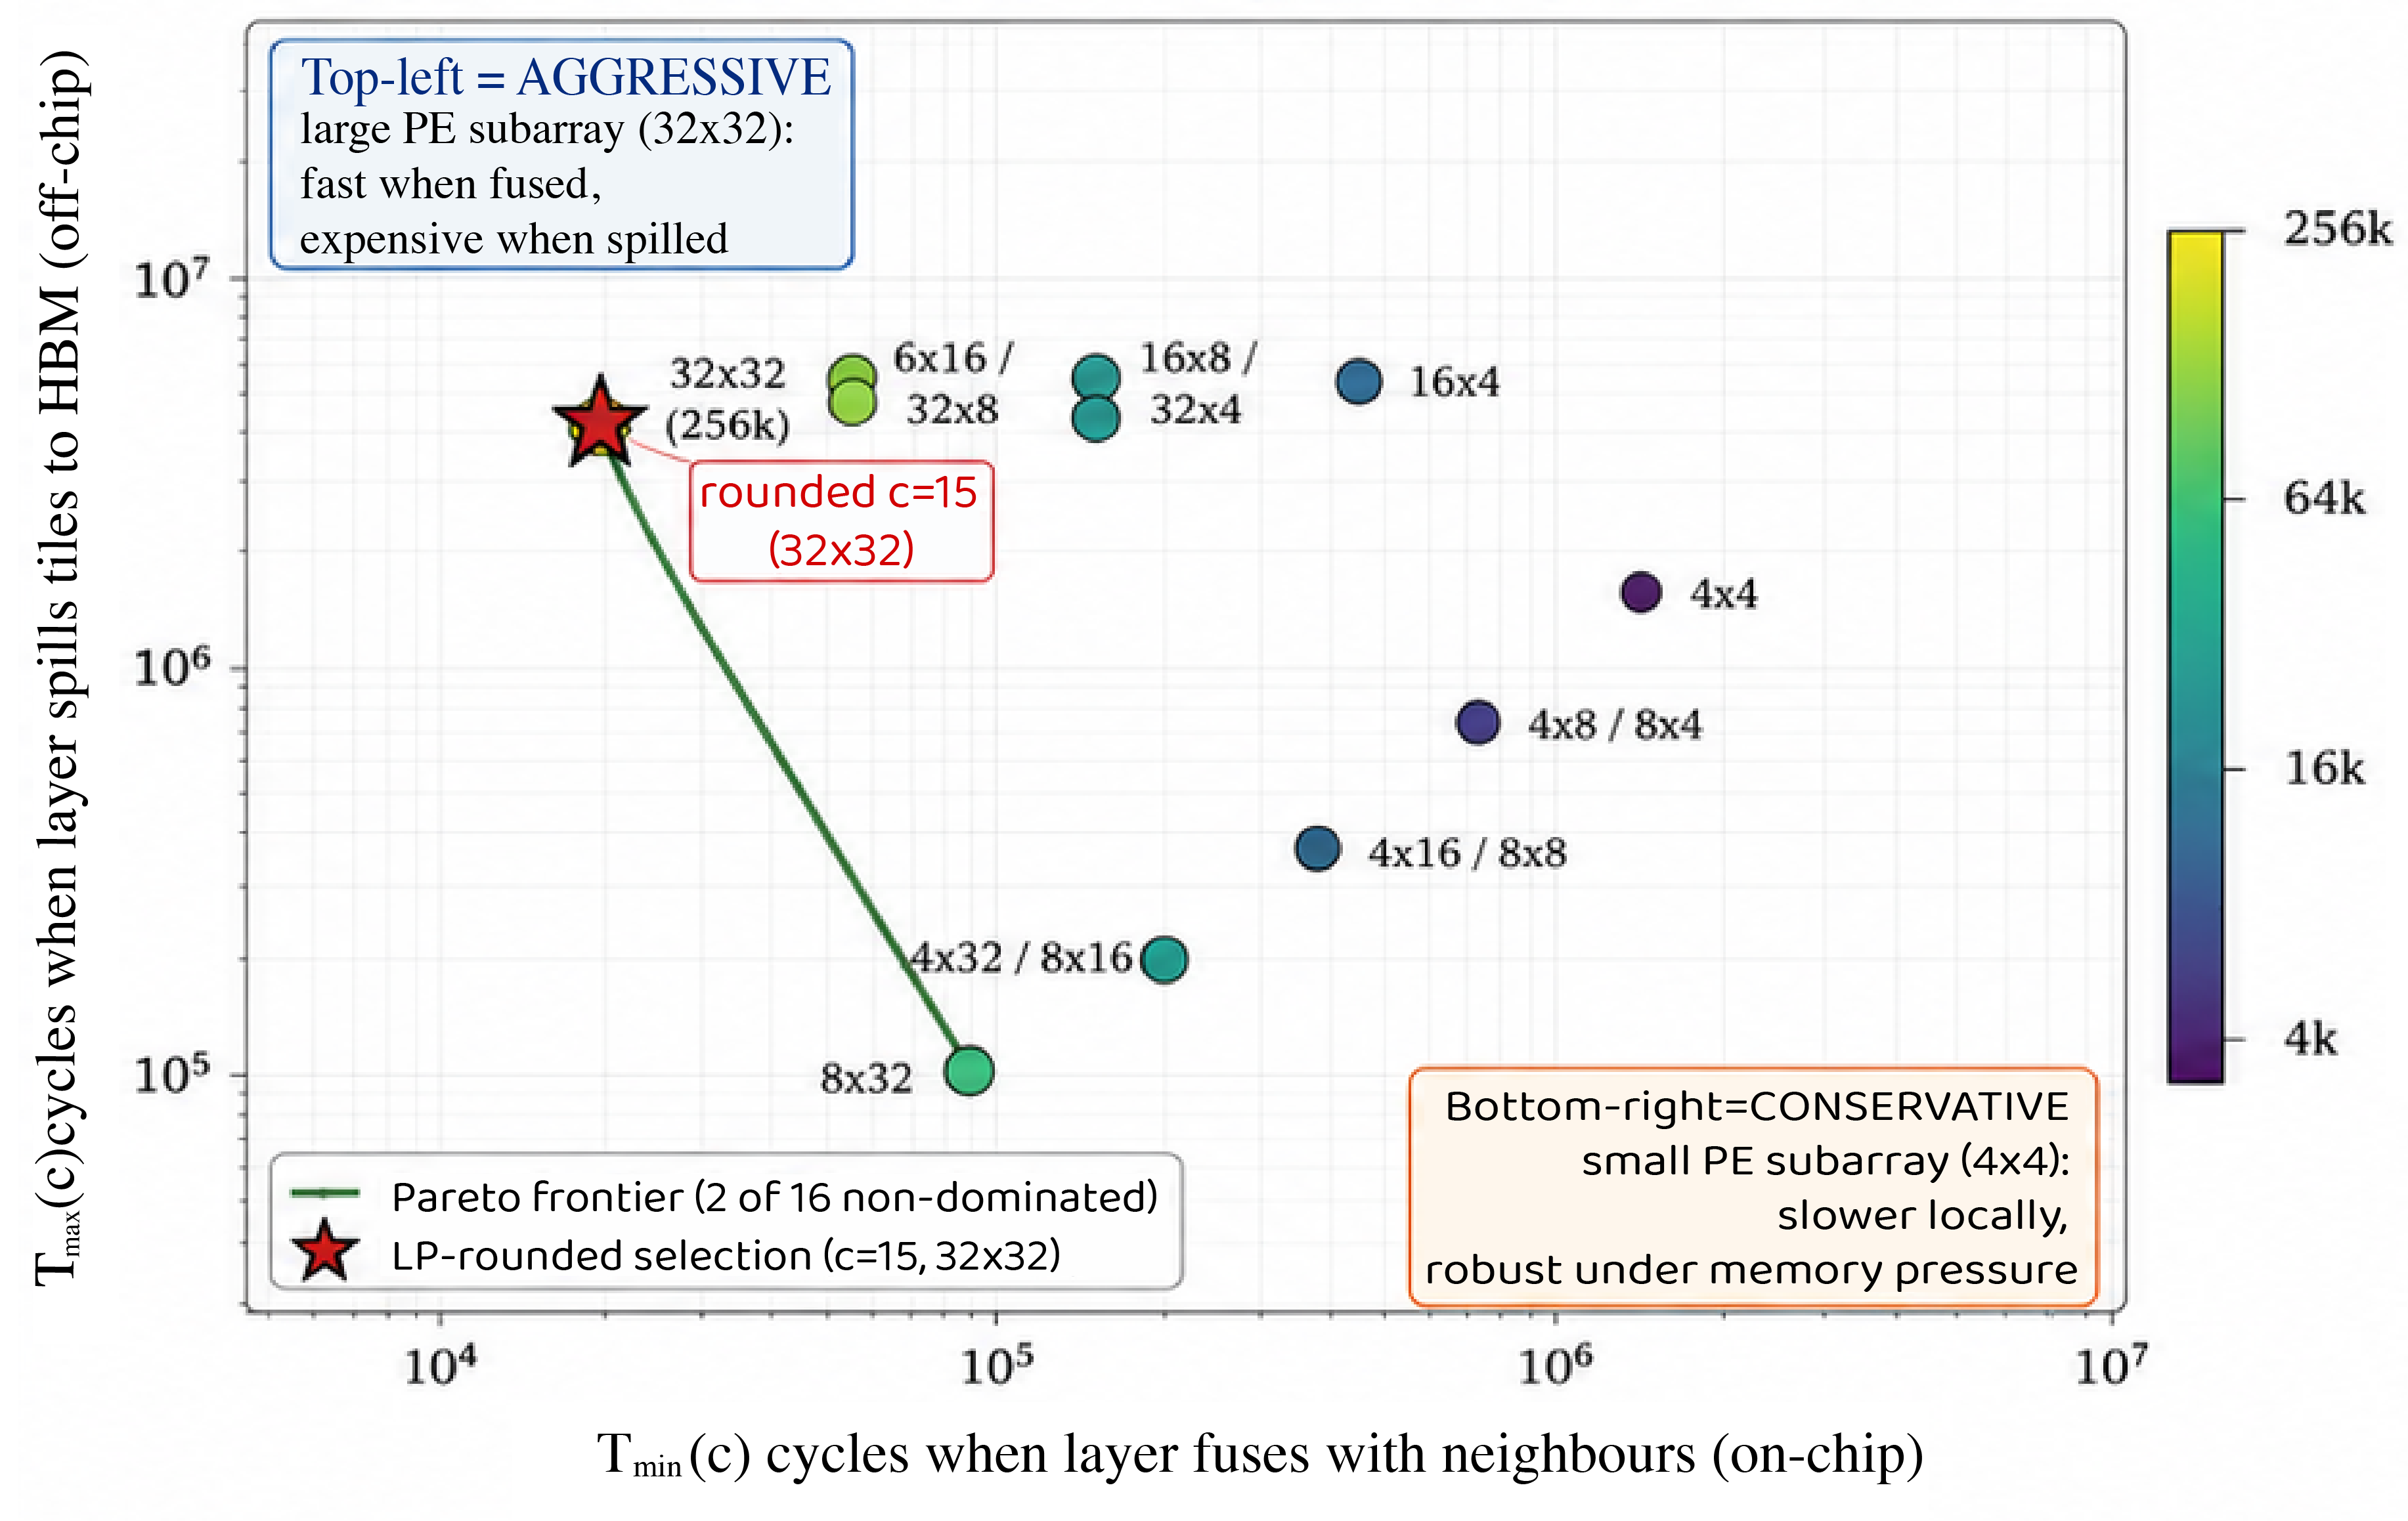
\includegraphics[width=0.48\textwidth]{figs4/pareto_front.png}
\hfill
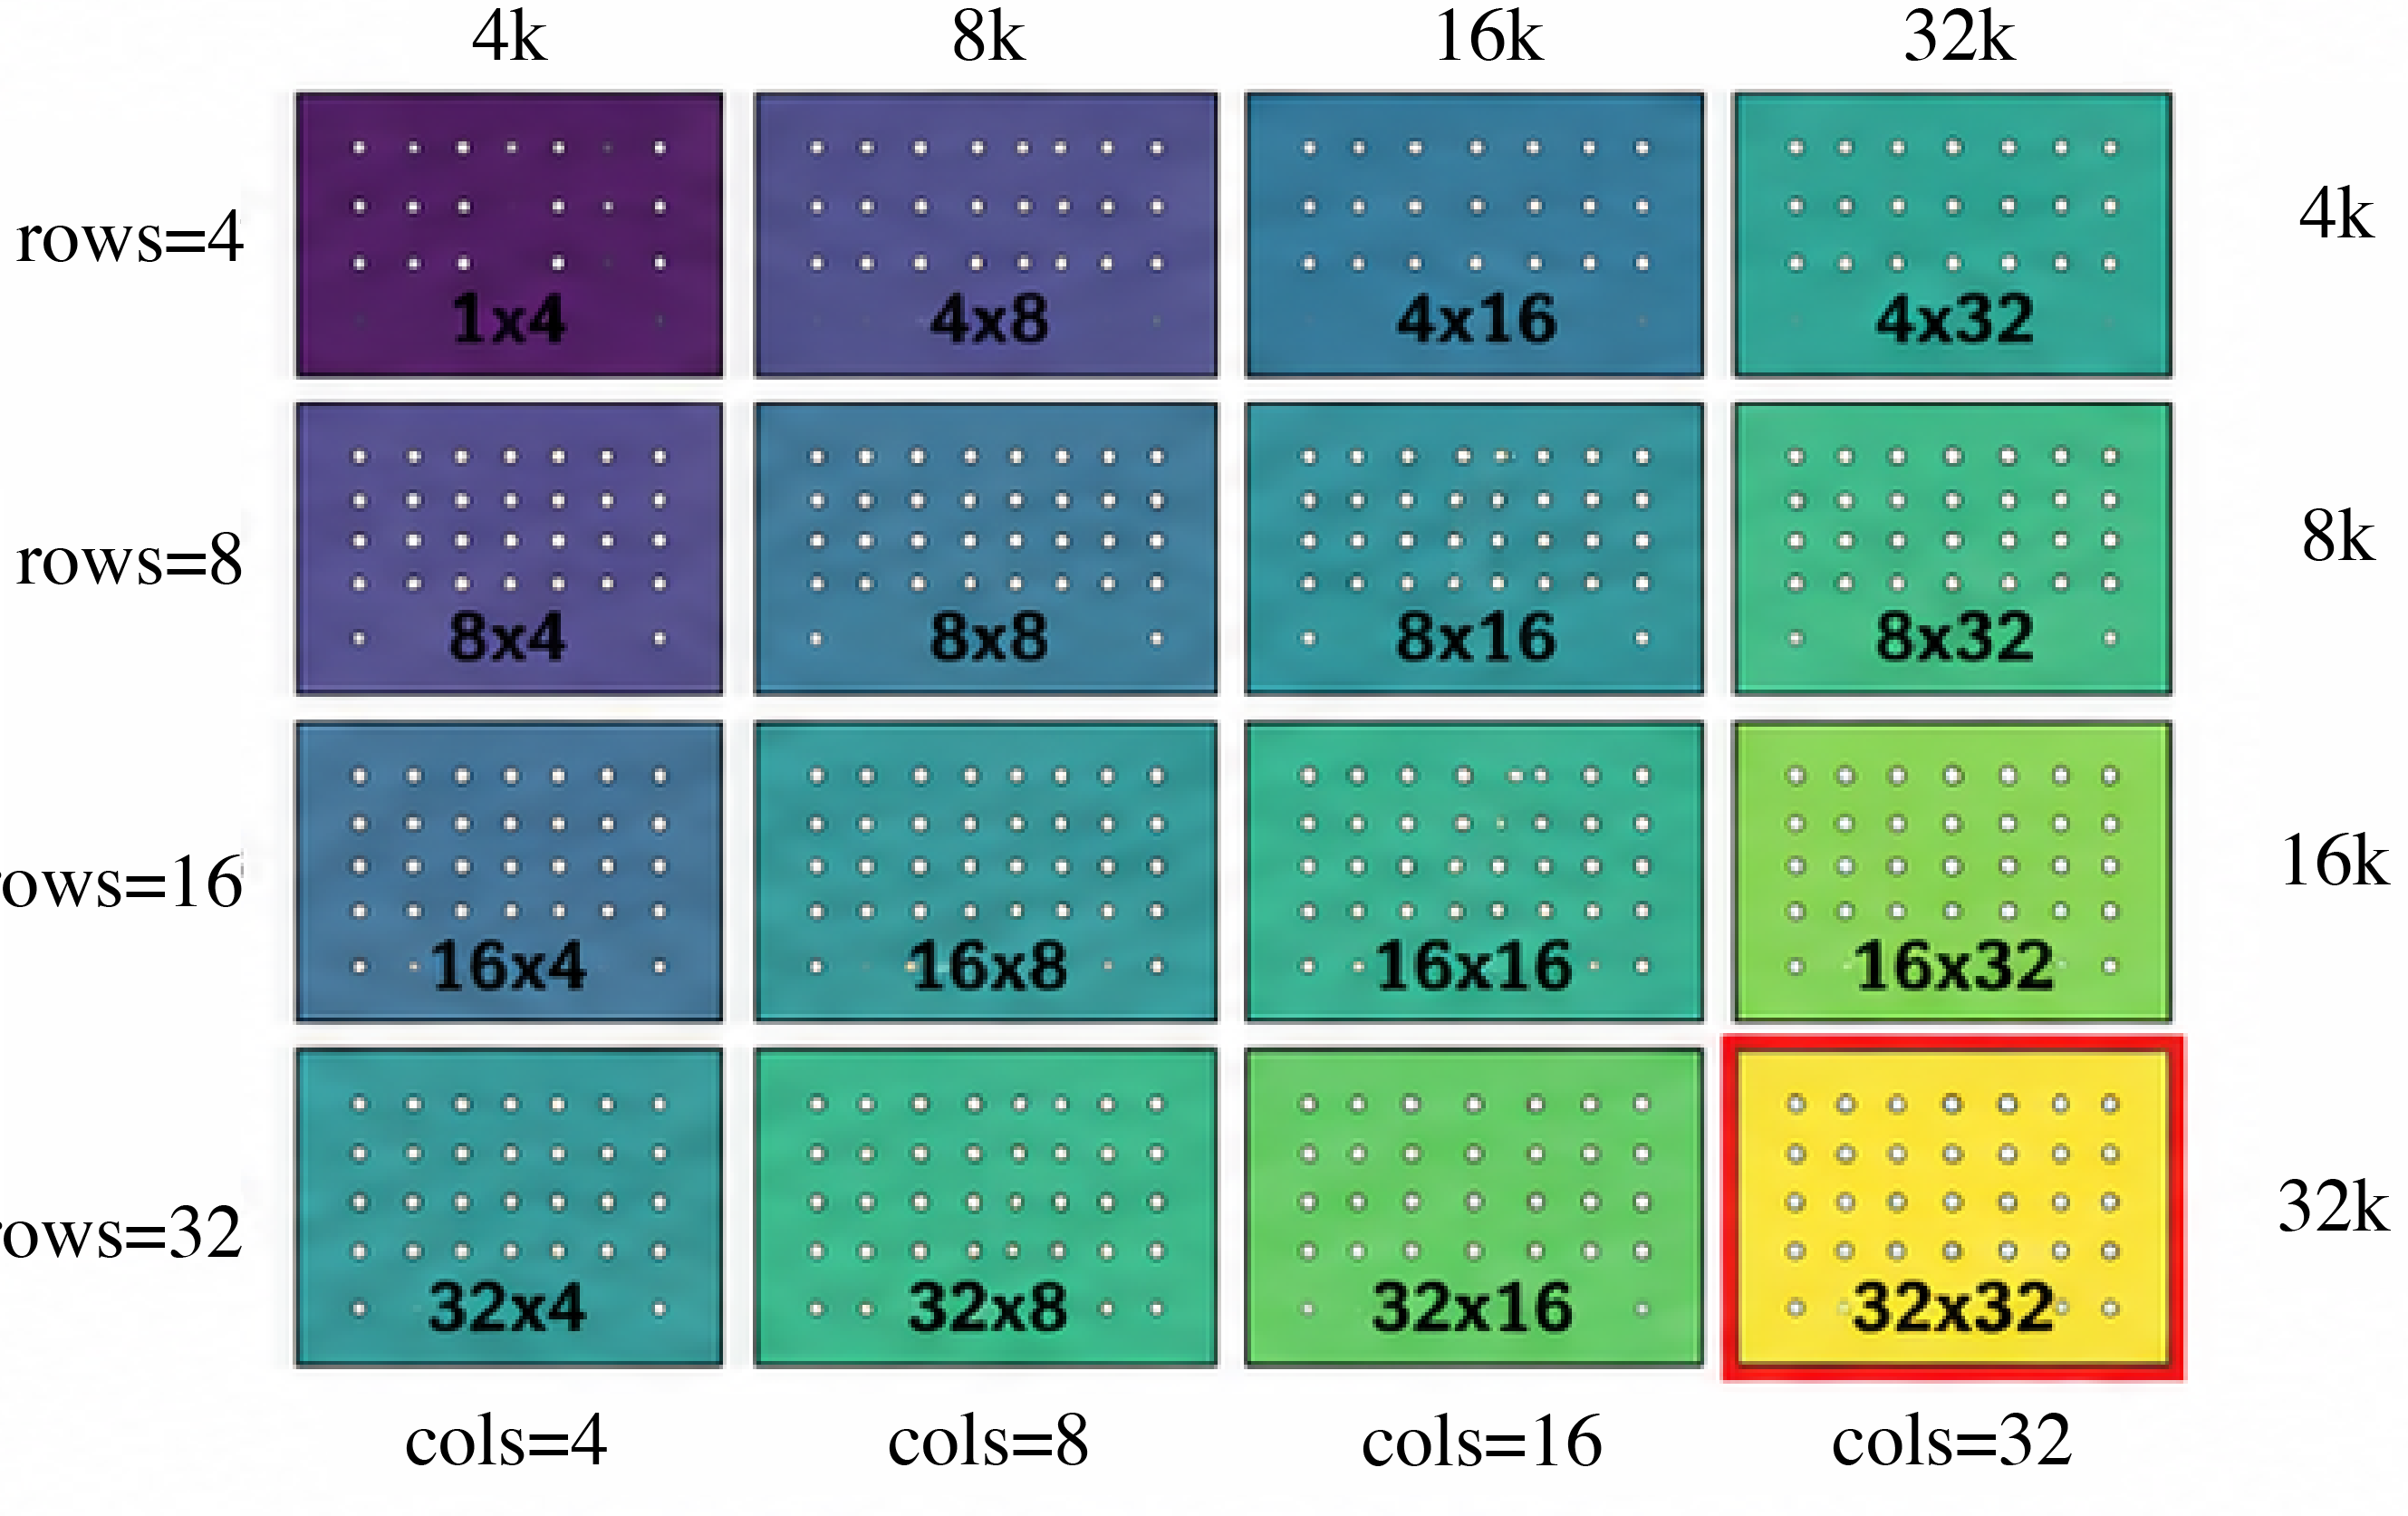
\includegraphics[width=0.48\textwidth]{figs4/tiles.png}
\caption{
Example per-layer tiling cache for EfficientNet-B7 layer L4.
Left: Timeloop-evaluated candidates plotted by fused/on-chip cost
\(T_{\min}(c)\) and spilled/off-chip cost \(T_{\max}(c)\); the frontier shows
non-dominated choices and the star is the LP-rounded selection. Right: the
16 tiling choices; labels such as \(4\times4\),
\(8\times8\), and \(32\times32\) denote active tile rows/columns inside the
fixed accelerator, white dots indicate active PE/MAC sites.
These are schedule choices, not different chips.
}
\label{fig:tiles}
\end{figure}

\paragraph{Per-layer joint candidate tiling advantage.}
For each operation, CHEETAH-V1 precomputes a small set of
Timeloop-evaluated tile mapping configurations and exposes them to the
V1 LP through the selection variables $y_{i,c}$.
Figure~\ref{fig:tiles} illustrates this for one layer: each point is one candidate mapping, with
$T_{\min}(c)$ on the $x$-axis representing the fused/on-chip execution
floor and $T_{\max}(c)$ on the $y$-axis representing the spilled/off-chip cost.
Aggressive mappings (upper left) are fast when fusion succeeds but
expensive, while conservative mappings (lower right) are
slower locally but more robust under memory pressure.
The LP relaxation assigns fractional mass to two configurations in this example,
$y_{15} = 0.71$ and $y_{11} = 0.29$, and the rounded replay selects
$c = 15$ (the $32\times32$ mapping), with only a $3\%$ gap to the LP
lower bound.

This illustrates one core advantage of the CHEETAH-V1 LP: tiling is no
longer fixed before fusion. Instead, tile choice, placement, and
rematerialization are jointly decided, and the solver is free
to choose a locally non-obvious mapping whenever doing so improves the
global schedule. 
Concretely, the V1 LP introduces $y_{i,c}$ alongside
McCormick auxiliary variables $w_{i,c,k}$ to make the tiling selection
interact directly with tensor placement and rematerialization decisions, with Timeloop running once per retained configuration to supply the
triple $\bigl(T_i^{\min}(c),\, T_i^{\max}(c),\, t_i^k(c)\bigr)$ for
each candidate~$c$.
% This demonstrates that by exploiting structural invariance and GPU-accelerated mathematical optimization, CHEETAH-V1 reduces the end-to-end co-design search time from days to under 2.2 hours—a ${\sim}93\%$ average reduction—while discovering architectural points that deliver up to $35\times$ speedup over the TPU-v3 baseline.

% Figure~\ref{fig:pareto} shows the Pareto frontier of best-achieved Perf/TDP versus wall-clock search cost. V1 strictly dominates both V0 and static at every time budget: within 10 minutes of search, V1 already exceeds the best Perf/TDP that V0 or static achieve after 60+ minutes. The V1 Pareto frontier reaches ${\sim}35\times$ Perf/TDP, roughly $3\times$ higher than the V0/static frontier at ${\sim}10\text{--}12\times$. This gap reflects two compounding advantages: V1 explores a strictly larger feasible region (joint tiling-fusion), and it eliminates Timeloop from the per-trial critical path, allowing more trials within any fixed time budget.


\paragraph{LLM Architect vs.\ Optimizer.} Modeled on SkyDiscovery~\citep{skydiscover2026}, the LLM Architect prunes
the outer search loop by proposing campaign patches rather than
predicting raw performance. It analyzes a Causal Ledger containing
invalid rates, MFU, and solver diagnostics to suggest constrained
hardware neighbourhoods for Vizier to explore locally. The V1 LP
remains the ground-truth evaluator, supported by a Roofline Auditor
that rejects physically impossible results.
In a widened search space, the LLM loop reduces invalid evaluations
from $24.5\%$ to $5.9\%$ on average to yield a $4.1\times$ reduction in wasted
trials (Figure~\ref{fig:llm}), while reaching the same optimal Perf/TDP scores as full-space
Vizier. This demonstrates that the LLM's role is steering Bayesian
optimization toward feasible, workload-appropriate subspaces rather than
replacing the solver. We provide exact prompts in Appendix~\ref{app:prompt} for full replication of results, as well as two specific case studies of real-world use cases.
\begin{figure}[ht!]
    \centering
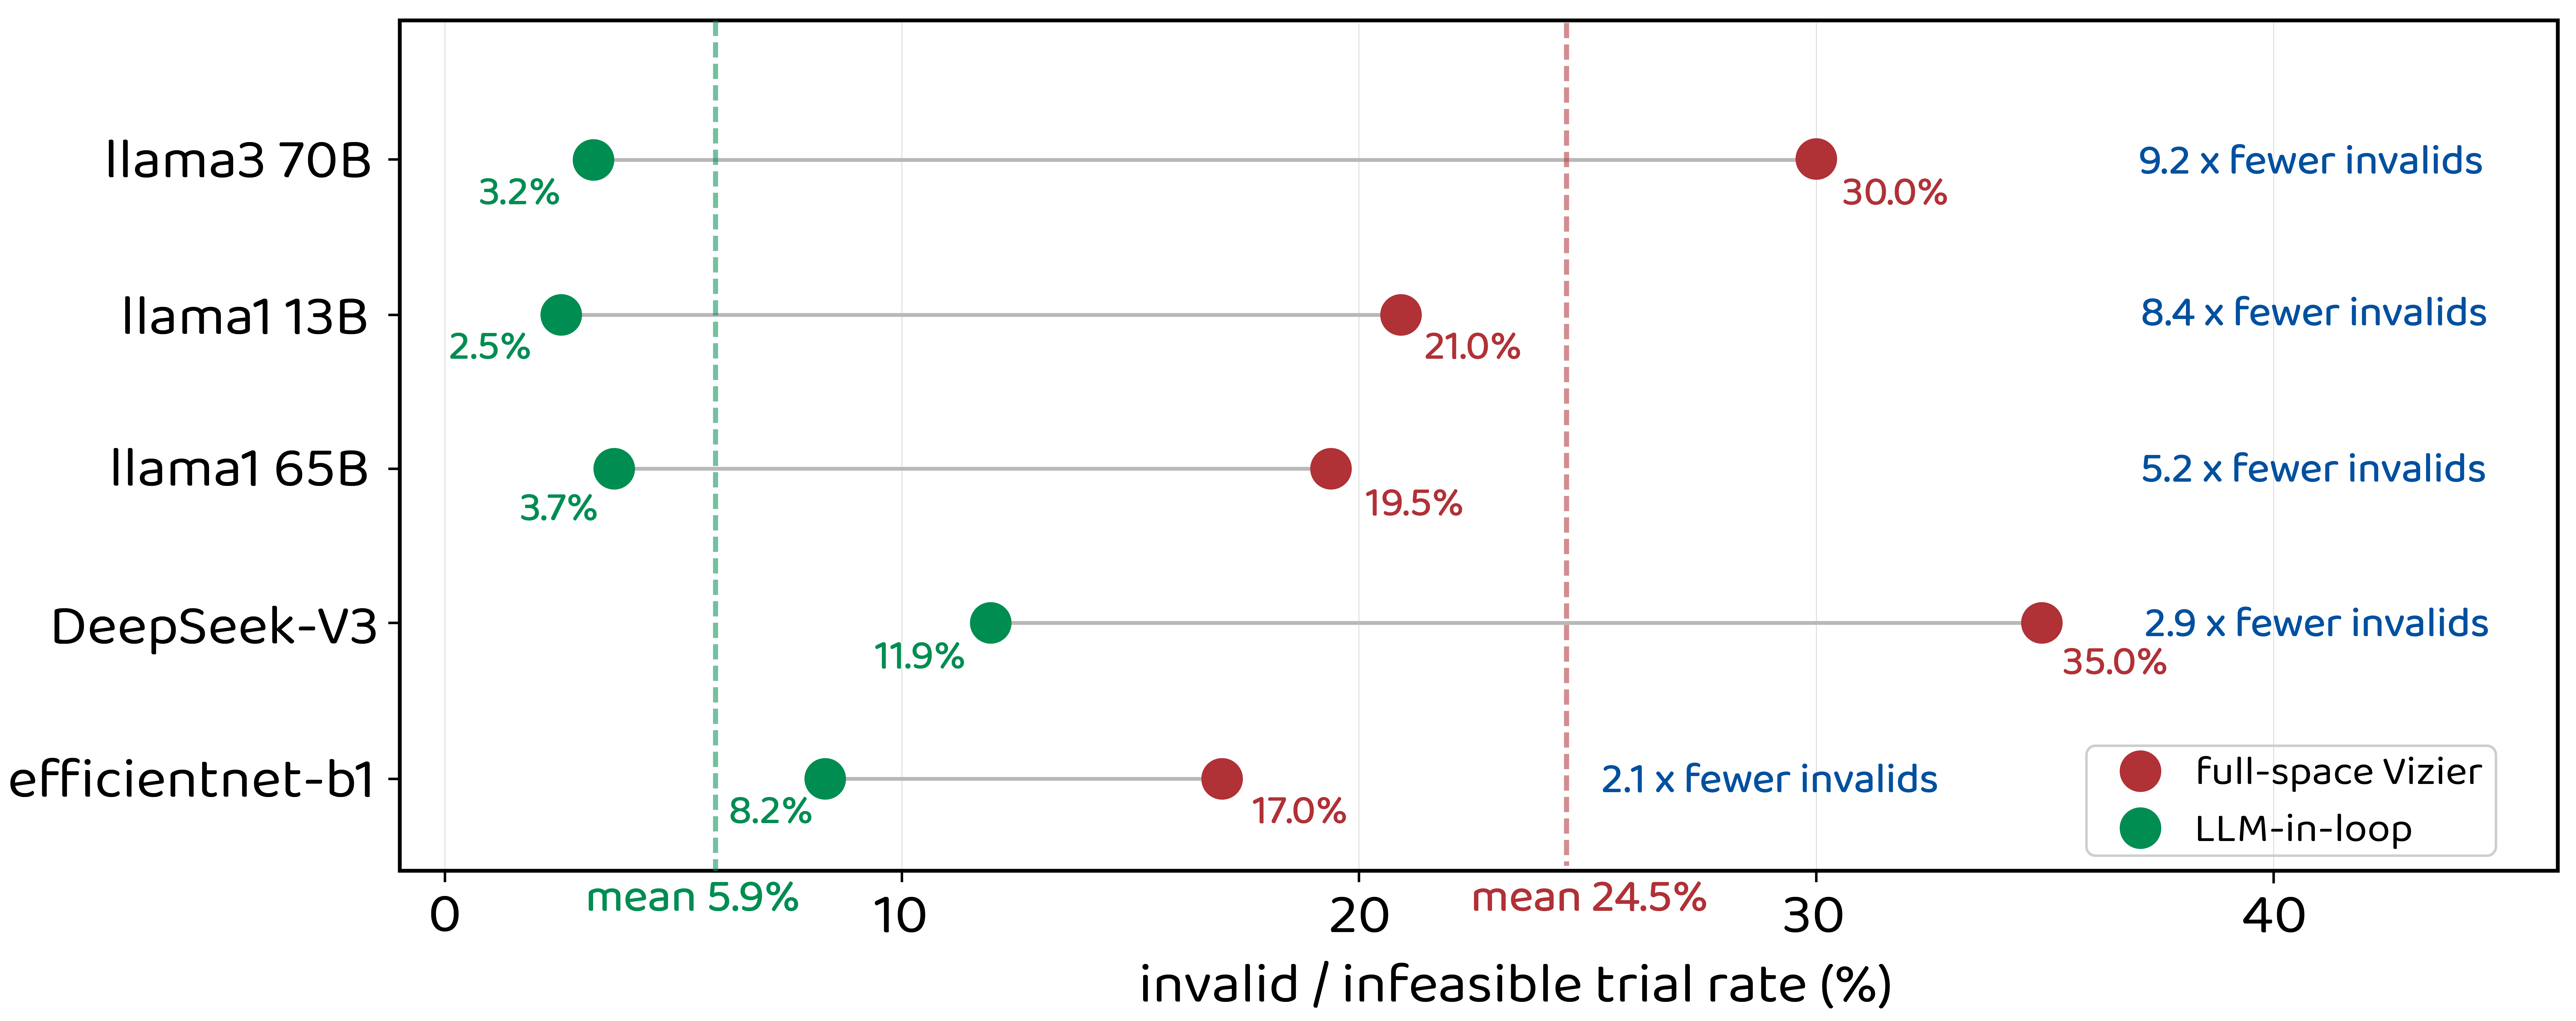
\includegraphics[width=0.85\linewidth]{fig3/llm_guide_v1.png}
\caption{Invalid/infeasible trial rate (\%) for full-space Vizier vs.\ LLM-in-loop across five workloads. The LLM Architect reduces the mean invalid rate from 24.5\% to 5.9\% (4.1$\times$ reduction), with the largest gains on LLM workloads where the hardware search space is most prone to infeasible configurations.}\label{fig:llm}
\end{figure}

% \subsection{Fixed Hardware + Dynamic Planning}

